\documentclass[11pt,a4paper]{article}
\usepackage[T1]{fontenc}
\usepackage[utf8]{inputenc}
\usepackage{lmodern}
\usepackage[margin=28mm]{geometry}
\usepackage{amsmath,amssymb,amsthm,mathtools,mathrsfs}
\usepackage{microtype}
\usepackage{booktabs,longtable,tabularx,array}
\usepackage{enumitem}
\usepackage{graphicx,xcolor,tikz}
\usetikzlibrary{arrows.meta,positioning,calc,decorations.pathreplacing,patterns}
\usepackage[hyphens]{url}
\usepackage[colorlinks=true,linkcolor=blue!45!black,citecolor=blue!45!black,
 urlcolor=blue!45!black,hypertexnames=false]{hyperref}
\usepackage{bookmark}
\allowdisplaybreaks[2]
\setlength{\emergencystretch}{3em}
\setlength{\parskip}{3pt}
\setcounter{tocdepth}{1}
\setlist{itemsep=2pt,topsep=4pt,parsep=0pt}
\setlist[enumerate,1]{label=\textup{(\roman*)}}

% ---------------------------------------------------------------- theorems
\newtheorem{theorem}{Theorem}[section]
\newtheorem{lemma}[theorem]{Lemma}
\newtheorem{proposition}[theorem]{Proposition}
\newtheorem{corollary}[theorem]{Corollary}
\newtheorem{maintheorem}{Theorem}
\renewcommand{\themaintheorem}{\Alph{maintheorem}}
\theoremstyle{definition}
\newtheorem{definition}[theorem]{Definition}
\newtheorem{example}[theorem]{Example}
\newtheorem{setup}[theorem]{Standing assumptions}
\theoremstyle{remark}
\newtheorem{remark}[theorem]{Remark}

% A visible but light marker for the steps of a long proof.
\newcommand{\step}[1]{\par\smallskip\noindent\textit{Step #1.}\ }

% ---------------------------------------------------------------- general
\newcommand{\R}{\mathbb R}
\newcommand{\T}{\mathbb T}
\newcommand{\Z}{\mathbb Z}
\newcommand{\av}[1]{\langle #1\rangle}
\newcommand{\dd}{\,d}
\newcommand{\id}{\mathrm{id}}
\newcommand{\supp}{\operatorname{supp}}
\newcommand{\dist}{\operatorname{dist}}
\newcommand{\diag}{\operatorname{diag}}
\newcommand{\Ai}{\operatorname{Ai}}
\newcommand{\Bi}{\operatorname{Bi}}

% ---------------------------------------------------------------- notation
% Symbols whose letters would otherwise collide are given macros, so
% that each has one meaning throughout the paper.
\newcommand{\jn}{\mathsf j}             % band edges  j_n = C_* q_n A_n^{-1/2}
\newcommand{\ea}{\mathsf a}             % coefficient exponent of sources
\newcommand{\eb}{\mathsf b}             % coefficient exponent of outputs
\newcommand{\el}{\mathsf l}             % intermediate loss exponent (Section 6)
\newcommand{\bd}{\mathsf d}             % boundary-defining function y(1-y)
\newcommand{\Dr}{\mathsf D}             % unit-scale radial derivative
\newcommand{\Qint}{\mathsf Q}           % integral functional on sources
\newcommand{\Odd}{\mathsf O}            % odd projection on the circle
\newcommand{\Even}{\mathsf E}           % even projection on the circle
\newcommand{\refl}{\mathsf s}           % reflection theta -> -theta
\newcommand{\Ev}{\mathsf{Ev}}           % even substitution at a root
\newcommand{\Od}{\mathsf{Od}}           % odd divided substitution at a root
\newcommand{\mA}{\mathsf A}             % matching matrices of Section 6
\newcommand{\mB}{\mathsf B}
\newcommand{\mK}{\mathsf K}
\newcommand{\mS}{\mathsf S}
\newcommand{\bx}{\mathbf x}             % the state (u,nu,kappa,h_L)
\newcommand{\bW}{\mathbf W}             % augmented canonical unknown

\newcolumntype{Y}{>{\raggedright\arraybackslash}X}
\hypersetup{pdftitle={Smooth isometric bending of a closed sphere},
 pdfauthor={Boyang Hu}}

\begin{document}
\begin{titlepage}
\centering
\vspace*{.22\textheight}
{\LARGE\bfseries Smooth isometric bending\\[.35em]of a closed sphere\par}
\vspace{2.5em}
{\large Boyang Hu\par}
\vspace{1em}
10 November 2026
\end{titlepage}
\begin{abstract}
We construct a smooth embedded sphere $\Sigma\subset\R^3$ together
with a smooth one-parameter family of isometric embeddings of $\Sigma$
whose images are not all congruent. The family is periodic; an inner
disk and a complementary cap stay fixed pointwise; and the area, the
enclosed volume and the total mean curvature do not change. This gives
a flexible closed surface in the smooth category.

The mechanism is elementary. A disk whose metric is rotationally
symmetric, but whose embedding is not, can be turned inside a fixed
shell provided it is exactly planar near its rim. The whole difficulty
is to produce such a disk. This reduces to a scalar equation of
Monge--Amp\`ere type on an annulus, the Darboux equation, for a height
function which must be nonradial and yet constant to infinite order at
both boundary circles.

We solve this equation by a Nash--Moser argument around an
infinitesimal bending of a radial profile. The profile is forced to
change the sign of its curvature infinitely often near each boundary
circle, so the linearized equation changes type on infinitely many
circles accumulating at both ends. We build the profile from explicitly
solvable one-dimensional models, describe its accumulating ends by an
exact three-term recurrence, and invert the linearized operator on the
whole annulus. Two modifications of the linearization, each
proportional to an unsolved equation, keep the type-change circles and
the characteristic return maps fixed during the iteration, so that all
linearized operators act on one domain.
\end{abstract}
\tableofcontents
\clearpage
\section{Introduction}
\label{sec:introduction}

\subsection{The result}

A \emph{bending} of a closed surface is a continuous family of
isometric embeddings of one fixed Riemannian metric into $\R^3$. It is
nontrivial when the shape of the surface changes, that is, when the
images are not all congruent. Connelly's flexible sphere
\cite{Connelly1977} shows that nontrivial bendings exist for embedded
polyhedra. Problem~1.1 of Ghomi's list \cite{Ghomi2019}, which is
attributed there to Euler and Maxwell, asks whether a closed $C^2$
surface in $\R^3$ can be flexible. We construct a $C^\infty$ example.

\begin{maintheorem}\label{thm:main}
There are a smooth surface $\Sigma$ diffeomorphic to $S^2$, a smooth
Riemannian metric $g_\Sigma$ on it, and a jointly smooth map
$\mathcal F:\Sigma\times\R\to\R^3$ such that the maps
$F_\tau=\mathcal F(\,\cdot\,,\tau)$ satisfy
\[
 F_\tau\text{ is an embedding},\qquad
 F_\tau^*g_{\mathrm E}=g_\Sigma,\qquad F_{\tau+1}=F_\tau
 \qquad\text{for all }\tau\in\R,
\]
where $g_{\mathrm E}$ is the Euclidean metric. At least two of the
images $F_\tau(\Sigma)$ are not congruent under the Euclidean isometry
group. An inner disk and a complementary cap of $\Sigma$ are fixed
pointwise throughout the family. The area, the enclosed volume and the
total oriented mean curvature of $F_\tau(\Sigma)$ do not depend on
$\tau$.
\end{maintheorem}

Three conventions are implicit in this statement. A \emph{closed}
surface is compact and without boundary. \emph{Nontrivial} always
refers to noncongruence of the images: relabelling the points of a
fixed surface by a family of intrinsic isometries moves material
points but does not change the shape, and is not a bending in our
sense. The mean curvature is $(k_1+k_2)/2$ for the outward normal.

\subsection{The mechanism}
\label{subsec:mechanism}

The family in Theorem~\ref{thm:main} is completely explicit once one
particular disk is available. Let $D$ be a disk with a rotationally
symmetric metric $g$, and write $\varrho_\vartheta$ for its intrinsic
rotation by the angle $\vartheta$. Suppose $F:D\to\R^3$ is an isometric
embedding. If $R_\vartheta$ denotes the rotation of $\R^3$ about the
vertical axis, then
\begin{equation}\label{eq:phase-family}
 F_\tau=R_{-2\pi\tau}\circ F\circ\varrho_{2\pi\tau}
\end{equation}
is again an isometric embedding of $(D,g)$ for every $\tau$, and its
image is the rotated copy $R_{-2\pi\tau}F(D)$ of the original image.
Two cases are uninteresting. If $F(D)$ is a surface of revolution,
the image does not move at all. If $F(D)$ is not a surface of
revolution, the image does move, but in general so does its boundary
curve, and nothing can be attached to it.

There is a third possibility. Suppose that $F(D)$ is not a surface of
revolution, but that near the boundary of $D$ the embedding is the
inclusion of a flat horizontal annulus, $F(x)=(x,c)$. There the two
rotations in \eqref{eq:phase-family} cancel, so $F_\tau=F$ near the
boundary for every $\tau$. All the maps $F_\tau$ can then be glued to
one and the same complementary cap. The result is a closed surface in
which a wavy annulus turns relative to a stationary shell
(Figure~\ref{fig:surface-motion}). If the shell carries a mark which
breaks its rotational symmetry, no rigid motion can account for the
relative rotation, and the shape of the closed surface changes.

\begin{figure}[htbp]
\centering
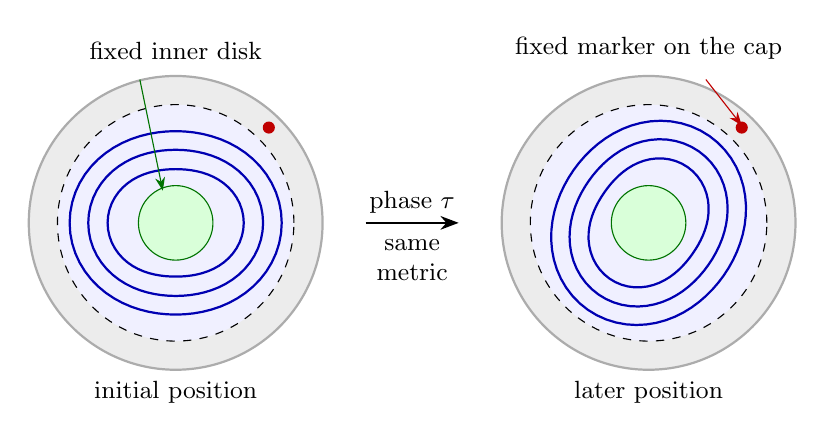
\begin{tikzpicture}[scale=.91,>=Stealth,font=\small]
\foreach \shift/\phase/\word in {0/0/initial,6.6/55/later}{
 \begin{scope}[xshift=\shift cm]
 \fill[gray!15] (0,0) circle (2.05);
 \fill[blue!6] (0,0) circle (1.65);
 \draw[gray!65,thick] (0,0) circle (2.05);
 \draw[dashed] (0,0) circle (1.65);
 \foreach \radius in {.85,1.12,1.38}{
  \draw[blue!70!black,thick,rotate=\phase]
   plot[domain=0:360,samples=65,variable=\t]
   ({(\radius+.10*cos(2*\t))*cos(\t)},
    {(\radius+.10*cos(2*\t))*sin(\t)});}
 \filldraw[fill=green!15,draw=green!45!black] (0,0) circle (.52);
 \fill[red!75!black] (1.30,1.33) circle (2.4pt);
 \node at (0,-2.36) {\word\ position};
 \end{scope}}
\draw[->,thick] (2.65,0)--(3.95,0);
\node[above] at (3.3,0) {phase $\tau$};
\node[below,align=center] at (3.3,-.1) {same\\metric};
\node[above] at (0,2.15) {fixed inner disk};
\draw[->,green!45!black] (-.5,2.0)--(-.18,.45);
\node[above] at (6.6,2.15) {fixed marker on the cap};
\draw[->,red!75!black] (7.4,2.0)--(7.90,1.36);
\end{tikzpicture}
\caption{The relative rotation, seen from above. The blue curves are
schematic height contours of the moving annulus; they are not numerical
data for the constructed surface. The dashed circle bounds the planar
collar, which stays fixed pointwise, as does the green inner disk. The
red marker on the cap also stays fixed while the nonradial part turns,
so no ambient rotation accounts for the whole motion.}
\label{fig:surface-motion}
\end{figure}

The motion itself therefore requires no analysis; in particular, no
infinitesimal bending has to be integrated in the variable $\tau$.
Everything rests on the existence of the disk, and the difficulty lies
in the requirement that it be \emph{exactly} planar on a collar of its
boundary while being nonradial inside.

\subsection{The analytic core}

Such a disk is produced as follows. Fill the middle of the disk by a
flat piece, so that only an annulus $(r_-,r_+)\times\T$ remains, where
$\T=\R/2\pi\Z$. On the annulus take the metric of a radial graph with
slope $w$,
\begin{equation}\label{eq:intro-metric-form}
 g=(1+w(r)^2)\,dr^2+r^2\,d\theta^2,
\end{equation}
and look for an isometric embedding of the form $(P,z)$, where $z$ is
a height function and $P$ takes values in the horizontal plane. Such
an embedding exists locally exactly when the \emph{remainder metric}
$g-dz\otimes dz$ is positive definite and flat, and flatness is a
single scalar equation for $z$, the Darboux equation. The disk of
Section~\ref{subsec:mechanism} is then obtained from the following
statement, which is the main analytic result of the paper.

\begin{maintheorem}\label{thm:annulus-intro}
There exist radii $0<r_-<r_+$, a smooth function $w>0$ on $(r_-,r_+)$
and a smooth function $z$ on $(r_-,r_+)\times\T$ with the following
properties, where $g$ is the metric \eqref{eq:intro-metric-form}.
\begin{enumerate}
\item $|dz|_g<1$, and the metric $g-dz\otimes dz$ is flat.
\item $z(r,\theta+\pi)=z(r,\theta)$, and $z$ is not independent of
 $\theta$.
\item $w$ extends smoothly by zero across $r_-$ and $r_+$, and $z$
 extends smoothly by a constant across each of them.
\end{enumerate}
\end{maintheorem}

Condition~(iii) says that $w$, and $z$ minus its boundary value, vanish
to infinite order at both boundary circles. After a slight enlargement
of the annulus this gives open collars on which $w=0$ and $z$ is
constant, which is the exact planarity needed for the mechanism. A
small error at the boundary would be useless; this is why flatness to
infinite order is the right target. The precise form of
Theorem~\ref{thm:annulus-intro}, with quantitative information on $w$
and $z$, is Theorem~\ref{thm:new-annular-height}.

The passage from Theorem~\ref{thm:annulus-intro} to
Theorem~\ref{thm:main} is carried out in
Section~\ref{sec:geometric-closure} and uses only classical
differential geometry. The rest of the paper proves
Theorem~\ref{thm:annulus-intro}.

\subsection{Three difficulties, and how they are met}
\label{subsec:difficulties}

We look for the height in the form $z=h+qu$, where $h'=w$ is the radial
height whose graph has the metric $g$, and $q$ is a small parameter. To
first order in $q$ the Darboux equation is
\begin{equation}\label{eq:intro-linear}
 \mathscr L_wu=(wu_r)_r+\frac{w'}{r}\,u_{\theta\theta}=0 .
\end{equation}
A nonzero solution of this equation which is constant to infinite order
at both ends is an infinitesimal version of what we want, and the plan
is to choose $w$ so that one exists and then to correct it to a
solution of the nonlinear equation. Three features of the problem shape
everything that follows.

\paragraph{Flat ends force infinitely many changes of type.}
For $w>0$ the operator \eqref{eq:intro-linear} is elliptic where $w'>0$
and hyperbolic where $w'<0$. At a flat end $w$ tends to zero. If $w$
were monotone near that end, no nonzero angular mode of
\eqref{eq:intro-linear} could vanish there together with its flux
(Proposition~\ref{prop:obs-monotone-tail}). So $w$ must oscillate: near
each end there are infinitely many circles on which the equation
changes type, and they accumulate at the boundary. We build such a
profile from infinitely many copies of one explicitly solvable cell,
with lengths and amplitudes decaying fast enough for smoothness
(Sections~\ref{sec:rosen-reference-packet} and~\ref{sec:radial-tails}).

\paragraph{Two unrelated resonance conditions.}
On each hyperbolic annulus, characteristics turn by a fixed
\emph{travel angle} $T$, and solving along them involves dividing by
$\sin(jT)$ at the angular frequency $j$. Independently, the solutions
on neighbouring annuli must be matched, and the matching fails at
eigenvalue-like resonances. A finite model in which both sets of
resonances can be computed exactly (Section~\ref{sec:worked-example})
shows that neither condition implies the other. In the actual profile
the travel angles are quadratic irrationals fixed by the choice of the
cells, while matching resonances are avoided by adjusting the relative
heights of consecutive cells. The outcome is a two-sided inverse of
$\mathscr L_w$ on the whole annulus, in spaces weighted towards the
flat ends (Section~\ref{sec:radial-reference-inverse}).

\paragraph{The inverse has to survive perturbation.}
The Nash--Moser method needs an inverse of the linearization at every
state near the reference one, not only at the reference. For a nearby
state both the type-change circles and the characteristic return maps
move, so its linearization does not even act on the same space. We
remove this problem by subtracting from the linearization two terms,
each proportional to an equation that is not yet solved: one fixes the
type-change circles, the other fixes the return maps. Both terms vanish
at a solution, and they produce exactly the quadratic error allowed by
Hamilton's form of the implicit function theorem \cite{Hamilton1982}
(Sections~\ref{sec:fixed-geometry}--\ref{sec:solving-the-equation}).

\subsection{Organization of the proof}
\label{subsec:organization}

Figure~\ref{fig:proof-map} shows the logical structure, and
Table~\ref{tab:sections} lists what each section contributes. The
paper has three parts.

\begin{figure}[htbp]
\centering
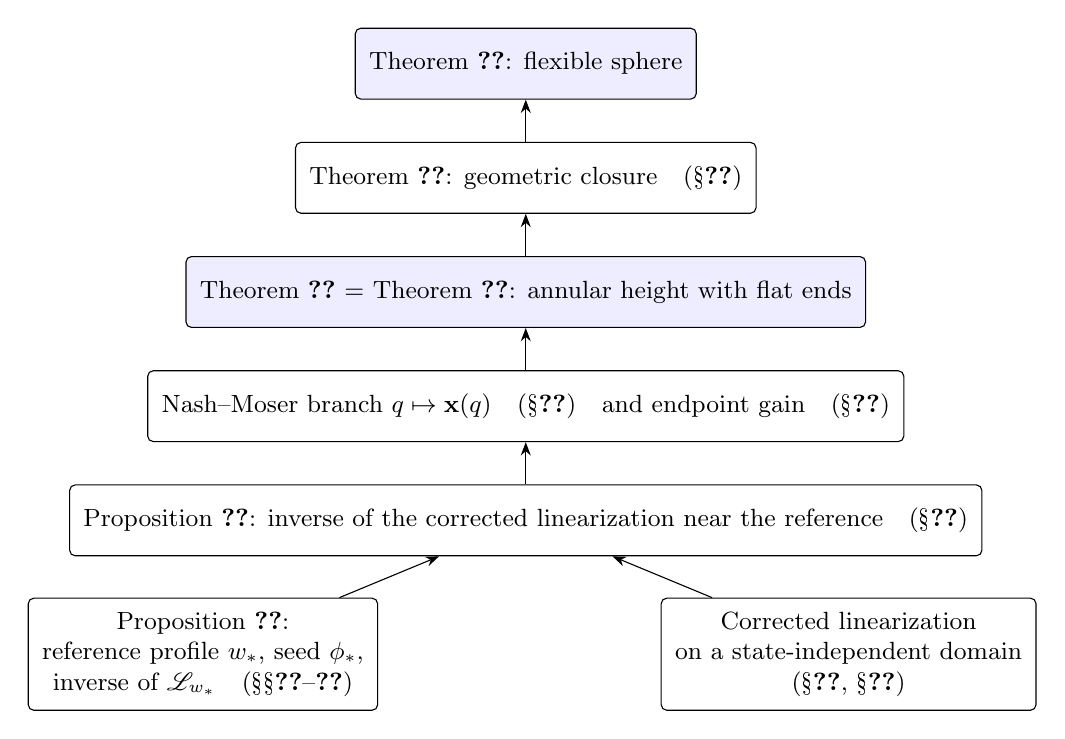
\begin{tikzpicture}[font=\small,>=Stealth,
 box/.style={draw,rounded corners=2pt,align=center,inner sep=5pt,
             minimum height=9mm}]
\node[box,fill=blue!7] (A) at (0,0)
 {Theorem~\ref{thm:main}: flexible sphere};
\node[box] (C) at (0,-1.45)
 {Theorem~\ref{thm:geometric-closure}: geometric closure\quad
  (\S\ref{sec:geometric-closure})};
\node[box,fill=blue!7] (B) at (0,-2.9)
 {Theorem~\ref{thm:annulus-intro} $=$
  Theorem~\ref{thm:new-annular-height}: annular height with flat ends};
\node[box] (N) at (0,-4.35)
 {Nash--Moser branch $q\mapsto\bx(q)$\quad
  (\S\ref{sec:solving-the-equation})\quad and endpoint gain\quad
  (\S\ref{sec:final-proof})};
\node[box] (I) at (0,-5.8)
 {Proposition~\ref{prop:rewrite-volume-inverse}: inverse of the
  corrected linearization near the reference\quad
  (\S\ref{sec:stable-inverse})};
\node[box] (R) at (-4.1,-7.5)
 {Proposition~\ref{prop:rad-fixed-theorem}:\\
  reference profile $w_*$, seed $\phi_*$,\\
  inverse of $\mathscr L_{w_*}$\quad
  (\S\S\ref{sec:rosen-reference-packet}--\ref{sec:radial-reference-inverse})};
\node[box] (F) at (4.1,-7.5)
 {Corrected linearization\\
  on a state-independent domain\\
  (\S\ref{sec:scalar-core}, \S\ref{sec:fixed-geometry})};
\draw[->] (C)--(A);
\draw[->] (B)--(C);
\draw[->] (N)--(B);
\draw[->] (I)--(N);
\draw[->] (R)--(I);
\draw[->] (F)--(I);
\end{tikzpicture}
\caption{The structure of the proof. An arrow means ``is used to
prove''.}
\label{fig:proof-map}
\end{figure}

\begin{table}[htbp]
\centering
\begin{tabularx}{\linewidth}{@{}l Y@{}}
\toprule
Section & What it provides\\
\midrule
\S\ref{sec:geometric-closure} &
 Theorem~\ref{thm:annulus-intro} implies Theorem~\ref{thm:main}:
 planar development, the marked cap, noncongruence, invariants.\\
\S\ref{sec:scalar-core} &
 The Darboux equation as the curvature of a connection form; its
 linearization and conservation law; why the ends must oscillate; the
 two resonances in a finite model; the first residual correction.\\
\S\ref{sec:rosen-reference-packet} &
 Statement of what the reference profile must provide
 (Proposition~\ref{prop:rad-fixed-theorem}); the two solvable models
 from which it is built.\\
\S\ref{sec:radial-tails} &
 The infinite chain of cells at each end; the mass--resistance
 recurrence and the decaying solution; choice of the cell heights.\\
\S\ref{sec:radial-reference-inverse} &
 The inverse of $\mathscr L_{w_*}$ on the whole annulus; proof of
 Proposition~\ref{prop:rad-fixed-theorem}.\\
\S\ref{sec:fixed-geometry} &
 Weighted spaces; the unknowns of the nonlinear problem; the second
 residual correction; coordinates in which every nearby linearization
 has the same transmission conditions.\\
\S\ref{sec:stable-inverse} &
 The inverse of the corrected linearization at nearby states, with tame
 estimates (Proposition~\ref{prop:rewrite-volume-inverse}).\\
\S\ref{sec:solving-the-equation} &
 The coupled linear system and Hamilton's theorem: a smooth branch of
 solutions.\\
\S\ref{sec:final-proof} &
 Improved decay of the metric corrections; the precise annular theorem
 (Theorem~\ref{thm:new-annular-height}); proof of
 Theorem~\ref{thm:main}.\\
Appendix~\ref{app:app-obstructions} &
 A side remark: no finite angular ansatz can solve the nonlinear
 equation.\\
Appendix~\ref{app:dependencies} &
 The external results in the form used, and the order in which the
 constants are chosen.\\
Appendix~\ref{app:notation} & Index of notation.\\
\bottomrule
\end{tabularx}
\caption{Contents by section.}
\label{tab:sections}
\end{table}

\emph{Part~\ref{part:geometry}} (Sections~\ref{sec:geometric-closure}
and~\ref{sec:scalar-core}) contains the geometry and the derivation of
the scalar equation. It is self-contained and elementary.

\emph{Part~\ref{part:reference}}
(Sections~\ref{sec:rosen-reference-packet}--\ref{sec:radial-reference-inverse})
is one-dimensional. After separation of angular modes, the linear
equation \eqref{eq:intro-linear} becomes a family of ordinary
differential equations, and the whole part is devoted to the
construction of one profile $w_*$ for which these equations have the
right kernel and a controlled inverse. Its only output is
Proposition~\ref{prop:rad-fixed-theorem}; a reader willing to accept
that proposition can go directly from Section~\ref{sec:radial-what}
to Part~\ref{part:nonlinear}.

\emph{Part~\ref{part:nonlinear}}
(Sections~\ref{sec:fixed-geometry}--\ref{sec:final-proof}) solves the
nonlinear equation near the reference and proves the two theorems.

The estimates are arranged so that precision is spent where the
decisions above are implemented: the matching of infinitely many
intervals, the common domain of the perturbed operators, and the decay
at the endpoints are proved in detail, while the spectra of the models
and the elementary operator theory are quoted. The specific numbers
that appear in the construction, such as the exponents $2n^3/3$ and
$n^{5/2}$, the power $12$ and the weight exponent $3/4$, are each
introduced together with the inequalities they have to satisfy; none
of them is optimal, and Table~\ref{tab:endpoint-budget} collects them.

\subsection{Context}

\paragraph{Continuous families versus pairs.}
Ghomi's problem \cite[Problem~1.1]{Ghomi2019} asks for a continuous
family. Replacing a dimple by its reflection across a flat rim gives
two different isometric realizations of one metric, but no path between
them. Theorem~\ref{thm:main} provides such a path in the smooth
category.

\paragraph{Infinitesimal versus finite bendings.}
A normal vector field supported inside a planar patch has zero first
variation of the metric. This observation already appears in
Cohn-Vossen's discussion of closed infinitesimally nonrigid surfaces
\cite[footnote~2]{CohnVossen1930}; it does not solve the nonlinear
isometry equations. Efimov's survey \cite{Efimov1948Survey} and his
work on deformations at points of zero curvature
\cite{Efimov1948Zero} belong to the historical setting of this
distinction, and the later survey
\cite[Sections~1.1--1.4]{IvanovaSabitov1991} treats finite bendings,
their infinitesimal equations and higher-order extension. Our starting
point is also an infinitesimal bending, the solution of
\eqref{eq:intro-linear}; the analysis of
Parts~\ref{part:reference} and~\ref{part:nonlinear} is what turns it
into an actual height.

\paragraph{Rigidity.}
On the rigid side, hypotheses on curvature and on boundary data are
decisive. For example, Ghomi and Spruck
\cite[Theorem~1.1]{GhomiSpruck2020} prove that two properly oriented
$C^{2,1}$ positively curved isometric immersions which agree on a curve
segment agree everywhere on their connected domain. The annulus of
Theorem~\ref{thm:annulus-intro} has curvature of both signs, with
infinitely many transitions at each flat end, so neither strict
positivity nor a finite collection of nondegenerate interfaces
describes its geometry.

\paragraph{Other categories.}
Connelly's flexible embedded polyhedral sphere \cite{Connelly1977}
establishes flexibility for polyhedra. Rounding its edges would change
the metric, so it does not furnish a smooth bending. The $C^1$ theorems
of Nash and Kuiper \cite{Nash1954,Kuiper1955} concern another
regularity regime; in the smooth problem the second fundamental form
and the type of the Darboux equation must be controlled at every scale.

\paragraph{Smooth isometric embedding.}
Our analytic method is closest to the theory of smooth isometric
embedding. Smoothing already compensates for the loss of derivatives in
Nash's argument \cite{Nash1956}. Han, Hong and Lin
\cite[Theorem~1.1]{HanHongLin2003} use a Nash--Moser--H\"ormander
scheme for nonpositive curvature under a specified degeneracy
condition, and Han and Khuri treat local problems of mixed type with
finite-order changes of type \cite{HanKhuri2010,HanKhuri2013}. In
particular, the modification of the linearization by a multiple of the
residual in \cite[pp.~650--653]{HanKhuri2010} is a precedent for our
residual corrections. The new issue here is the simultaneous control of
infinitely many interfaces and of both flat ends on a single closed
domain.

\paragraph{The invariants.}
The three invariants in Theorem~\ref{thm:main} follow directly from the
form \eqref{eq:phase-family} of the motion. They should be compared
with general results of different scope: Sabitov's volume theorem
\cite{Sabitov1996} is polyhedral, and Almgren and Rivin
\cite{AlmgrenRivin1998} prove the invariance of the mean-curvature
integral under smooth bendings. Motions in which curvature precesses
around a shell also arise in the mechanical model of Hamouche, Maurini,
Vidoli and Vincenti \cite{Hamouche2017}; that comparison supplies
neither the flat collars nor the closed embedded surface.

\subsection{Conventions}
\label{subsec:conventions}

Throughout, $\T=\R/2\pi\Z$, the angular average of a function is
\[
 \av f=\frac1{2\pi}\int_0^{2\pi}f\,d\theta ,
\]
and $R_\vartheta$ denotes a rotation by the angle $\vartheta$, of the
plane, of $\R^3$ about the vertical axis, or of the circle
($R_\vartheta\theta=\theta+\vartheta$), as the context requires. A
prime denotes a derivative with respect to the radius $r$ unless
another variable is indicated by a subscript.

The letters $C$ and $c$ denote positive constants, large and small
respectively, whose values may change from line to line; a subscript
indicates dependence, as in $C_s$. We write $a\asymp b$ when
$cb\le a\le Cb$. Constants that are fixed once and referred to later
carry a distinguishing mark, as in $C_*$, $c_0$ or $N$.

The paper uses a fairly large number of symbols. Each of
Parts~\ref{part:reference} and~\ref{part:nonlinear} begins by fixing
its vocabulary, and Appendix~\ref{app:notation} is an index of
notation. Some letters have a local meaning inside a single proof;
this is always said where it happens.


\part{The mechanism and the equation}
\label{part:geometry}
\section{From an annular height to a flexible sphere}
\label{sec:geometric-closure}

This section proves that Theorem~\ref{thm:annulus-intro} implies
Theorem~\ref{thm:main}. It uses no analysis beyond the classical
theory of surfaces, and it fixes exactly what the remaining sections
have to construct. The steps are as follows.
\begin{itemize}
\item An isometric embedding with prescribed height $z$ exists locally
 if and only if the remainder metric $g-dz\otimes dz$ is positive and
 flat (Lemma~\ref{lem:darboux-invariant}).
\item On a disk whose rim is planar, a positive flat remainder metric
 develops onto a round disk, and the development is the identity near
 the rim (Proposition~\ref{lem:disk-development}).
\item The resulting graph is closed by a cap which carries a marker
 (Lemma~\ref{lem:fixed-cap}).
\item Turning the graph inside the cap gives the family of
 Theorem~\ref{thm:main} (Theorem~\ref{thm:geometric-closure}).
\end{itemize}

\subsection{Setting}

Throughout the section $0<r_-<r_+$, and on the annulus
$(r_-,r_+)\times\T$ with coordinates $(r,\theta)$ we consider a metric
\begin{equation}\label{eq:intro-metric}
 g=E(r)\,dr^2+r^2\,d\theta^2,\qquad E=1+w^2,
\end{equation}
where $w$ is a smooth function of $r$. This is the metric induced on
the graph $(r\cos\theta,r\sin\theta,h(r))$ of a radial function with
$h'=w$. We identify $(r,\theta)$ with the point
$x=(r\cos\theta,r\sin\theta)$ of the plane, and write $D_\rho$ for the
closed disk of radius $\rho$ centred at the origin.

\begin{definition}\label{def:flat-endpoint}
A smooth function $f$ on $(r_-,r_+)$, or on $(r_-,r_+)\times\T$, is
\emph{flat} at an endpoint if it extends smoothly by zero across that
endpoint; equivalently, every derivative of $f$ tends to zero there. A
function $z$ has a \emph{constant extension} at an endpoint if $z$ has
a limit $c$ there, independent of $\theta$, and $z-c$ is flat.
\end{definition}

If $w$ is flat and $z$ has constant extensions at both endpoints, we
may extend $w$ by zero and $z$ by its limits, and regard them as
defined on a slightly larger annulus. On the added collars $w=0$ and
$z$ is constant. All statements of this section are therefore
formulated for functions which are constant on open collars of the two
ends.

\subsection{Removing one coordinate from the metric}

A map $F=(P,z)$ into $\R^2\times\R$ is isometric for $g$ exactly when
\[
 P^*g_{\R^2}=\bar g,\qquad \bar g:=g-dz\otimes dz .
\]
Thus $\bar g$ must be a positive definite flat metric, and for an
embedding its planar development $P$ must be injective. Flatness is a
scalar equation for $z$. For a symmetric $2$-tensor $B$ we write
$\det_gB=\det(B_{ij})/\det(g_{ij})$, and $\nabla_g^2z$ is the Hessian
of $z$ for the metric $g$.

\begin{lemma}[Darboux equation]\label{lem:darboux-invariant}
Let $z$ be a smooth function on a surface with metric $g$, and assume
$\sigma:=|dz|_g^2<1$. Then $\bar g=g-dz\otimes dz$ is positive
definite, and its curvature is
\begin{equation}\label{eq:darboux-curvature}
 K_{\bar g}=
 \frac{K_g(1-\sigma)-\det_g\nabla_g^2z}{(1-\sigma)^2}.
\end{equation}
In particular $\bar g$ is flat if and only if
\begin{equation}\label{eq:intro-darboux}
 \det\nolimits_g\nabla_g^2z=K_g\,(1-|dz|_g^2).
\end{equation}
\end{lemma}

\begin{proof}
In a $g$-orthonormal coframe $(e^1,e^2)$ with $dz=\sqrt\sigma\,e^1$ we
have $\bar g=(1-\sigma)\,e^1\otimes e^1+e^2\otimes e^2$. This is
positive definite, and $|dz|_{\bar g}^2=\sigma/(1-\sigma)$.

Consider the product $(\Sigma,\bar g)\times\R$ and in it the graph
$x\mapsto(x,z(x))$. The metric induced on the graph is
$\bar g+dz\otimes dz=g$. Its upward unit normal has vertical component
$(1+|dz|_{\bar g}^2)^{-1/2}=\sqrt{1-\sigma}$. The vertical coordinate
is a function on the product with vanishing Hessian, and its restriction
to the graph is $z$; hence the intrinsic Hessian of $z$ is the second
fundamental form $\mathrm{II}$ of the graph times the vertical
component of the normal,
\[
 \nabla_g^2z=\sqrt{1-\sigma}\;\mathrm{II}.
\]
The sectional curvature of the product on the tangent plane of the
graph is $K_{\bar g}$ times the squared area distortion of the
horizontal projection, which is $1-\sigma$. The Gauss equation for the
graph therefore reads
\[
 K_g=(1-\sigma)K_{\bar g}+\det\nolimits_g\mathrm{II}
    =(1-\sigma)K_{\bar g}+(1-\sigma)^{-1}\det\nolimits_g\nabla_g^2z ,
\]
and solving for $K_{\bar g}$ gives \eqref{eq:darboux-curvature}.
\end{proof}

Equation~\eqref{eq:intro-darboux} is thus exactly the compatibility
condition for the two horizontal coordinates once the vertical
coordinate has been chosen. It guarantees local developments. The
global reconstruction, including injectivity, is the subject of the
next proposition; no local embedding theorem is used to bypass it.

\subsection{Development onto a round disk}

A flat metric on an annulus may have nontrivial holonomy around the
hole. Filling the inner collar by a flat disk removes the holonomy,
and the half-turn symmetry of $z$ forces the inner disk to stay
centred.

\begin{proposition}[Planar reconstruction]\label{lem:disk-development}
Suppose that $w$ vanishes on open collars of both ends of
$(r_-,r_+)$, that $z$ equals a constant $c_L$ on the inner collar and
a constant $c_R$ on the outer one, and that
$z(r,\theta+\pi)=z(r,\theta)$. Suppose that $\bar g=g-dz\otimes dz$ is
positive definite and flat. Extend $w$ by $0$ and $z$ by $c_L$ to
$r\le r_-$. Then there is an orientation-preserving diffeomorphism
$P:D_{r_+}\to D_{r_+}$ such that
\[
 P^*g_{\R^2}=\bar g,
 \qquad P=\id\ \text{on the outer collar},
 \qquad P=R_\gamma\ \text{on the inner disk }D_{r_-}
\]
for some angle $\gamma$. Consequently $F=(P,z):D_{r_+}\to\R^3$ is an
isometric embedding of $(D_{r_+},g)$, and its image is a graph over
$D_{r_+}$.
\end{proposition}

\begin{proof}
\step{1: a normalized development}
On the inner disk and on the outer collar we have $w=0$ and $dz=0$, so
there $\bar g=g=dr^2+r^2d\theta^2$ is the Euclidean metric in the
coordinate $x$. In particular $\bar g$ is a smooth flat metric on the
whole disk $D_{r_+}$, including its centre. Choose a global oriented
$\bar g$-orthonormal coframe $\eta_1,\eta_2$ which equals $dx_1,dx_2$
on the outer collar, and let $\alpha$ be its connection form:
$d\eta_1=\alpha\wedge\eta_2$, $d\eta_2=-\alpha\wedge\eta_1$. Flatness
means $d\alpha=0$, and since the disk is simply connected,
$\alpha=d\psi$ with $\psi=0$ on the outer collar. The complex form
$e^{i\psi}(\eta_1+i\eta_2)$ is then closed. Its primitive $P$,
normalized to be the identity on the outer collar, is an
orientation-preserving local isometry from $(D_{r_+},\bar g)$ to the
plane.

\step{2: the inner disk is rotated about its centre}
Two orientation-preserving local isometries from a connected flat
surface to the plane differ by a fixed Euclidean motion; this follows
by differentiating their relative rotation. Let $I(x)=-x$ be the
half-turn. It preserves $\bar g$ because $g$ is rotationally symmetric
and $z\circ I=z$. Both $P$ and $-P\circ I$ are orientation-preserving
local isometries equal to the identity on the outer collar, so they
coincide: $P$ is odd. On the inner disk $\bar g$ is Euclidean, hence
$P$ is a Euclidean motion there, and an odd Euclidean motion is a
rotation $R_\gamma$ about the origin.

\step{3: $P$ is a diffeomorphism of the disk}
Extend $P$ by the identity outside $D_{r_+}$. The extension is a local
diffeomorphism of $\R^2$ which is the identity outside a compact set;
it is proper, hence a covering map, and it has one sheet because it is
injective near infinity. So it is a diffeomorphism of $\R^2$, and
since it fixes the exterior of the disk it maps $D_{r_+}$ onto itself.

\step{4: conclusion}
The map $F=(P,z)$ is injective because $P$ is, and its induced metric
is $P^*g_{\R^2}+dz\otimes dz=\bar g+dz\otimes dz=g$. Its image is the
graph of $z\circ P^{-1}$ over $D_{r_+}$.
\end{proof}

\begin{figure}[htbp]
\centering
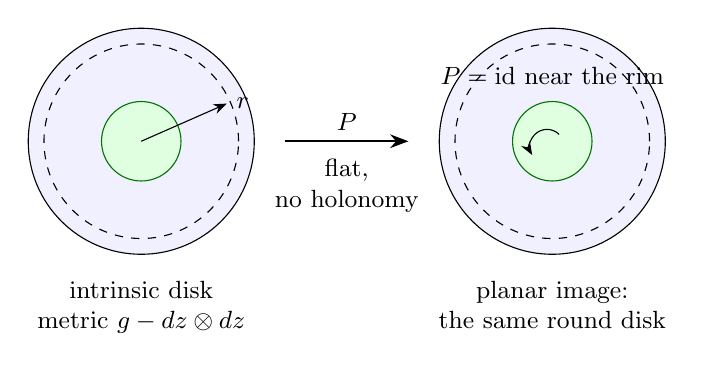
\begin{tikzpicture}[scale=.87,>=Stealth,font=\small]
\begin{scope}
\filldraw[fill=blue!6,draw=black] (0,0) circle (1.65);
\filldraw[fill=green!12,draw=green!45!black] (0,0) circle (.58);
\draw[dashed] (0,0) circle (1.42);
\draw[->] (0,0)--(1.25,.55) node[right] {$r$};
\node[below,align=center] at (0,-1.9) {intrinsic disk\\metric $g-dz\otimes dz$};
\end{scope}
\draw[->,thick] (2.1,0)--(3.9,0) node[midway,above] {$P$};
\node[align=center] at (3,-.65) {flat,\\no holonomy};
\begin{scope}[xshift=6cm]
\filldraw[fill=blue!6,draw=black] (0,0) circle (1.65);
\filldraw[fill=green!12,draw=green!45!black] (0,0) circle (.58);
\draw[dashed] (0,0) circle (1.42);
\draw[->] (.1,.1) arc[start angle=45,end angle=210,radius=.25];
\node at (0,.95) {$P=\id$ near the rim};
\node[below,align=center] at (0,-1.9) {planar image:\\the same round disk};
\end{scope}
\end{tikzpicture}
\caption{The development $P$. Filling the inner collar removes the
holonomy of the annulus; the normalization fixes the outer collar; the
half-turn symmetry keeps the inner disk centred, so that $P$ only
rotates it. Properness upgrades the local development to a
diffeomorphism. The sketch records these constraints, not the
pointwise distortion of $P$.}
\label{fig:development}
\end{figure}

\subsection{A stationary cap which distinguishes shapes}

The graph of Proposition~\ref{lem:disk-development} is horizontal near
its boundary, so it can be closed by a cap. A rotationally symmetric
cap would hide the relative rotation: the closed surfaces obtained for
different $\tau$ would be congruent. We therefore put on the cap a
marker which is recognized by every congruence.

\begin{lemma}[The marked cap]\label{lem:fixed-cap}
Let $S_0$ be a smooth graph over $D_{r_+}$ which is horizontal near its
boundary. Then $S_0$ extends to a smooth embedded sphere $S_0\cup S_1$.
The complementary cap $S_1$ can be chosen so that, for any given
constant $K_{\max}$, it contains a point $p$ with
\[
 K(p)>K_{\max},\qquad K(p)>K(p')\ \text{ for every other point }p'
 \text{ of }S_1,
\]
and with distinct principal curvatures at $p$.
\end{lemma}

We shall take $K_{\max}$ to be the maximum of the Gaussian curvature
of $S_0$. Then $p$ is the unique point of the closed surface at which
the Gaussian curvature is largest.

\begin{proof}
\step{1: the unmarked cap}
Translate so that the boundary height is zero, and extend the
horizontal collar to a radius $R>r_+$. Choose a smooth nondecreasing
function $\chi:[0,1]\to[0,1]$ which is $0$ near $0$, is $1$ near $1$,
and satisfies $\chi(1-t)=1-\chi(t)$. For $L>0$ consider the unit-speed
meridian curve $s\mapsto(r(s),z(s))$, $0\le s\le L$, which starts at
$(R,0)$ and satisfies
\[
 r'(s)=\cos(\pi\chi(s/L)),\qquad
 z'(s)=-\sin(\pi\chi(s/L)).
\]
Its tangent turns from the outward horizontal direction to the inward
one. By the symmetry of $\chi$ the curve stays at radius at least $R$
and returns to radius $R$, and its height decreases by a positive
constant times $L$. Take $L$ so large that the curve ends below the
minimum of the graph $S_0$, and complete it by the horizontal segment
from its endpoint to the axis. Rotating this meridian gives a smooth
embedded surface which meets $S_0$ only along the attaching collar.

\step{2: the marker}
Place a bump in the horizontal annulus $r_+<r<R$. In Cartesian
coordinates $(x,y)$ centred at a point of that annulus, choose
constants $A,B>0$ with $A\ne B$, and $k,\rho>0$; put $\xi=Ax^2+By^2$
and
\[
 u(x,y)=\frac{k}{2}\int_\xi^{\rho^2}
       e^{-s/(\rho^2-s)}\,ds\quad(\xi<\rho^2),
 \qquad u=0\quad(\xi\ge\rho^2).
\]
This function is smooth. With $\Xi=\xi/(\rho^2-\xi)$ one computes
$u_x=-kAx\,e^{-\Xi}$ and $u_y=-kBy\,e^{-\Xi}$, and the Gaussian
curvature of the graph of $u$ is
\begin{equation}\label{eq:marker-curvature}
 K=\frac{ABk^2e^{-2\Xi}\,(1-2\xi\,\Xi')}
 {\bigl[1+k^2e^{-2\Xi}(A^2x^2+B^2y^2)\bigr]^2},
 \qquad \Xi'=\frac{d\Xi}{d\xi}>0 .
\end{equation}
At the centre $K=ABk^2$. At every other point of the support the
numerator is either nonpositive or strictly smaller than $ABk^2$, and
the denominator is at least one. So the centre $p$ is the unique
maximum of $K$ on the bump, with value $ABk^2$. First choose $k$ so
that $ABk^2$ exceeds both $K_{\max}$ and the curvature of the unmarked
cap. Then choose $\rho$ so small that the support $\{\xi<\rho^2\}$
fits inside the horizontal annulus; the bump has height at most
$k\rho^2/2$ and does not meet the rest of the surface. At $p$ the
gradient of $u$ vanishes and its Hessian is $\diag(-kA,-kB)$, so the
principal curvatures are $-kA$ and $-kB$ for the upward normal. They
are distinct.
\end{proof}

\begin{figure}[htbp]
\centering
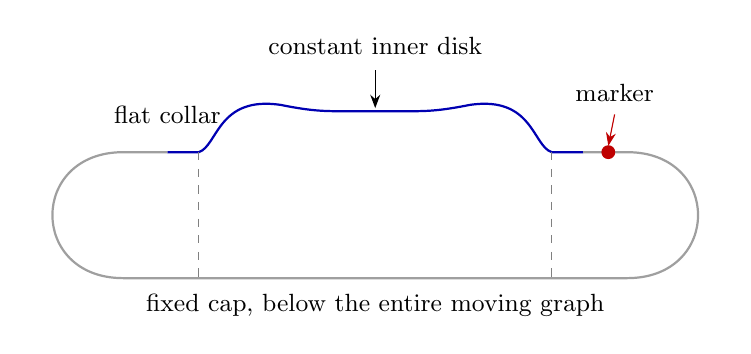
\begin{tikzpicture}[x=.8cm,y=.8cm,>=Stealth,font=\small]
\draw[thick,blue!70!black]
 (-3.3,0)--(-2.8,0) .. controls (-2.5,.1) and (-2.5,.9) .. (-1.5,.75)
 .. controls (-1,.65) and (-.8,.65) .. (-.5,.65)--(.5,.65)
 .. controls (.8,.65) and (1,.65) .. (1.5,.75)
 .. controls (2.5,.9) and (2.5,.1) .. (2.8,0)--(3.3,0);
\draw[thick,gray!75] (3.3,0)--(4,0)
 .. controls (5.5,0) and (5.5,-2) .. (4,-2)--(-4,-2)
 .. controls (-5.5,-2) and (-5.5,0) .. (-4,0)--(-3.3,0);
\fill[red!75!black] (3.7,0) circle (2.5pt);
\draw[dashed,gray] (-2.8,0)--(-2.8,-2);
\draw[dashed,gray] (2.8,0)--(2.8,-2);
\node[above] at (0,1.4) {constant inner disk};
\draw[->] (0,1.3)--(0,.7);
\node[above] at (-3.3,.3) {flat collar};
\node[above] at (3.8,.65) {marker};
\draw[->,red!75!black] (3.8,.6)--(3.7,.1);
\node[below] at (0,-2.1) {fixed cap, below the entire moving graph};
\end{tikzpicture}
\caption{A meridional sketch of the closed surface. The blue graph
depends on the angle; all its rotated copies stay inside the central
cylinder and above the bottom of the cap. The marker lies in the
stationary horizontal extension of the collar.}
\label{fig:geometric-closure}
\end{figure}

\subsection{The annulus implies the theorem}

\begin{theorem}[Geometric closure]\label{thm:geometric-closure}
Let $g$ be a metric of the form \eqref{eq:intro-metric} and let $z$ be
a smooth function on the annulus. Suppose that
\begin{enumerate}
\item $w=0$ on open collars of both ends, and $z$ is constant on each
 of these collars;
\item $z(r,\theta+\pi)=z(r,\theta)$, and $z$ is not independent of
 $\theta$;
\item $g-dz\otimes dz$ is positive definite and flat.
\end{enumerate}
Then all the conclusions of Theorem~\ref{thm:main} hold.
\end{theorem}

\begin{proof}
\step{1: the family}
Let $P$ and $F=(P,z)$ be given by
Proposition~\ref{lem:disk-development}, and attach to the graph
$F(D_{r_+})$ the marked cap of Lemma~\ref{lem:fixed-cap}, with
$K_{\max}$ the maximum of the Gaussian curvature of $F(D_{r_+})$. Let
$\Sigma$ be the resulting sphere, with its induced metric $g_\Sigma$.
On the disk put
\[
 F_\tau=R_{-2\pi\tau}\circ F\circ\varrho_{2\pi\tau},\qquad
 \varrho_\vartheta(r,\theta)=(r,\theta+\vartheta),
\]
and let $F_\tau$ be the inclusion on the cap. The intrinsic rotation
$\varrho_\vartheta$ preserves $g$, so each $F_\tau$ is isometric on
the disk. On the outer collar $F(x)=(x,c_R)$, and on the inner disk
$F(x)=(R_\gamma x,c_L)$; in both cases the two rotations cancel and
$F_\tau=F$. Hence $F_\tau$ agrees with the inclusion near the rim and
is smooth on $\Sigma$, jointly in the point and in $\tau$, and
$F_{\tau+1}=F_\tau$. The image $F_\tau(D_{r_+})=R_{-2\pi\tau}F(D_{r_+})$
is a graph over the same round disk with the same range of heights, so
it meets the cap only along the collar: $F_\tau$ is an embedding. The
inner disk and the cap are fixed pointwise.

\step{2: the disk images are not all equal}
Suppose $R_\vartheta F(D_{r_+})=F(D_{r_+})$ for every $\vartheta$. Then
$F^{-1}\circ R_\vartheta\circ F$ is an isometry of $(D_{r_+},g)$, and
on the outer collar it equals $\varrho_\vartheta$. An isometry of a
connected Riemannian manifold is determined by its value and
differential at one point, so $F^{-1}R_\vartheta F=\varrho_\vartheta$
on the whole disk. Comparing the vertical components of
$R_\vartheta F=F\varrho_\vartheta$ gives
$z(r,\theta+\vartheta)=z(r,\theta)$ for all $\vartheta$, contrary to
assumption~(ii).

\step{3: the closed images are not all congruent}
The Gaussian curvature of $F_\tau(\Sigma)$ is determined by
$g_\Sigma$, so by the choice of the marker the point $p$ is, for every
$\tau$, the unique point of $F_\tau(\Sigma)$ of largest Gaussian
curvature; it lies on the cap and is the same point of $\R^3$ for all
$\tau$. Let $\Phi$ be a Euclidean isometry mapping $F_0(\Sigma)$ onto
$F_\tau(\Sigma)$. It preserves the Gaussian curvature, so
$\Phi(p)=p$. It maps the bounded component of the complement to the
bounded component, so it preserves the outward normal at $p$, and then
it preserves each of the two principal directions at $p$, which are
well defined because the principal curvatures are distinct and which
are the same for all $\tau$ because the cap is fixed. There are at
most four such isometries. Thus, if all the images were congruent, the
family $\tau\mapsto F_\tau(\Sigma)$ would be a continuous family of
compact sets taking values in a finite set, hence constant. The part
of $F_\tau(\Sigma)$ inside the closed cylinder over $D_{r_+}$ and above
the bottom of the cap is $F_\tau(D_{r_+})$, so the disk images would
all be equal, which Step~2 excludes.

\step{4: the invariants}
The area is constant because the metric is. The moving part
$F_\tau(D_{r_+})$ is a rotated copy of $F(D_{r_+})$ and the rest of
the surface is stationary, so the integral of the oriented mean
curvature is constant. Finally let $Z_\tau$ be the height of
$F_\tau(D_{r_+})$ as a graph over $D_{r_+}$, and let $c_B$ be the
height of the bottom of the cap. The part of the enclosed volume
inside the cylinder over $D_{r_+}$ is
\[
 \int_{D_{r_+}}(Z_\tau(y)-c_B)\,dy
 =\int_{D_{r_+}}(Z_0(R_{2\pi\tau}y)-c_B)\,dy
 =\int_{D_{r_+}}(Z_0(y)-c_B)\,dy,
\]
and the remaining volume is bounded by the stationary part of the
surface.
\end{proof}

\begin{proof}[Proof that Theorem~\ref{thm:annulus-intro} implies
Theorem~\ref{thm:main}]
Let $w$ and $z$ be as in Theorem~\ref{thm:annulus-intro}. Extend $w$
by zero and $z$ by its two limiting constants to a slightly larger
annulus. The extended functions are smooth, and on the added collars
$g-dz\otimes dz=g$ is Euclidean, hence positive and flat. All the
hypotheses of Theorem~\ref{thm:geometric-closure} hold.
\end{proof}

What remains is therefore precise: construct one nonradial height on
an annulus with a positive flat remainder metric and with constant
extensions at both ends. The family of embeddings then follows without
any further existence argument.

\section{The height equation}
\label{sec:scalar-core}

The geometric reduction leaves two things to choose: the rotational
metric, that is the slope $w$, and the nonradial height $z$. This
section derives the equation that relates them and extracts from it
the information that guides both choices.
\begin{itemize}
\item Section~\ref{subsec:residual} writes the curvature of the
 remainder metric as the exterior derivative of a connection form.
 This gives the equation, its linearization in divergence form, and a
 conservation law.
\item Section~\ref{subsec:monotone} shows that a flat end at which $w$
 is monotone carries no infinitesimal bending. This is why the profile
 must oscillate.
\item Section~\ref{sec:worked-example} computes, in a finite model, the
 two different resonance sets mentioned in the introduction.
\item Section~\ref{subsec:normalization} normalizes the equation in
 the small parameter, and Section~\ref{subsec:first-correction}
 introduces the first of the two residual corrections.
\end{itemize}

\subsection{The curvature residual and its derivative}
\label{subsec:residual}

Let $h$ be a radial function with $h'=w$, so that $g$ in
\eqref{eq:intro-metric} is the metric of its graph and $E=1+w^2$. For
a height $z(r,\theta)$ we use the abbreviations
\begin{equation}\label{eq:height-jet-notation}
 k=z_r,\qquad p=\frac{z_\theta}{r},\qquad
 D=E(1-p^2)-k^2,\qquad Q=k+Ep_\theta .
\end{equation}
In the coordinates $(r,\theta)$ the remainder metric
$\bar g=g-dz\otimes dz$ has determinant $r^2D$, and
$1-|dz|_g^2=D/E$. Hence
\[
 \bar g\ \text{is positive definite}
 \iff D>0\iff |dz|_g<1 .
\]
We call $D$ the \emph{discriminant}. When $D>0$, an oriented
$\bar g$-orthonormal coframe is
\[
 \eta_1=\frac{\sqrt D}{\sqrt{1-p^2}}\,dr,\qquad
 \eta_2=r\sqrt{1-p^2}\,d\theta-\frac{kp}{\sqrt{1-p^2}}\,dr .
\]
For the radial height $z=h$ it reduces to the polar coframe
$dr,\ r\,d\theta$ of the plane, whose connection form is $d\theta$.

All adjoints of scalar operators in this paper are taken with respect
to $dr\,d\theta$, and source terms are densities for this measure. The
measure will be written out whenever coordinates are changed.

\begin{proposition}[Connection form, residual, linearization]
\label{prop:scalar-core}
Assume $D>0$.
\begin{enumerate}
\item The connection form $\alpha$ of the coframe $(\eta_1,\eta_2)$,
 defined by $d\eta_1=\alpha\wedge\eta_2$ and
 $d\eta_2=-\alpha\wedge\eta_1$, is
 \begin{equation}\label{eq:conn-one-form}
  \alpha=D^{-1/2}\left(d\theta+\frac{k}{1-p^2}\,dp\right).
 \end{equation}
\item Define the \emph{curvature residual}
 $\mathcal N_h(z)=-\sqrt D\,K_{\bar g}$. Then
 $d\alpha=r\,\mathcal N_h(z)\,dr\wedge d\theta$ and
 \begin{equation}\label{eq:cart-curvature-scalar}
  r\,\mathcal N_h(z)=D^{-3/2}
  \left[Qk_r-Er\,p_r^2-\frac{E'}2\,(1-p^2+kp_\theta)\right].
 \end{equation}
 In particular $\bar g$ is flat if and only if
 \begin{equation}\label{eq:darboux-numerator}
  Qk_r-Er\,p_r^2-\frac{E'}2\,(1-p^2+kp_\theta)=0 .
 \end{equation}
\item For fixed $w$, the derivative of the residual in the direction
 $\eta$ is in divergence form,
 \begin{equation}\label{eq:cart-true-derivative}
  r\,D_z\mathcal N_h(z)\,\eta
   =\partial_r(a\eta_r+b\eta_\theta)
       +\partial_\theta(b\eta_r+c\eta_\theta),
 \end{equation}
 with coefficients
 \begin{equation}\label{eq:linear-coefficients}
  a=\frac{Q}{D^{3/2}},\qquad b=-\frac{Ep_r}{D^{3/2}},\qquad
  c=\frac{Ek_r-E'k/2}{r\,D^{3/2}} .
 \end{equation}
\item The determinant of the coefficient matrix is
 \begin{equation}\label{eq:cart-determinant-identity}
  ac-b^2=\frac{K_0}{D^2}+\frac{E}{D^{3/2}}\,\mathcal N_h(z),
  \qquad K_0=\frac{ww'}r .
 \end{equation}
\end{enumerate}
\end{proposition}

\begin{proof}
Equality of mixed derivatives of $z$ gives the compatibility relation
\begin{equation}\label{eq:height-compatibility}
 r\,p_r=k_\theta-p .
\end{equation}

\step{1: the connection form}
Write $\alpha=\alpha_r\,dr+\alpha_\theta\,d\theta$. The second
structure equation determines $\alpha_\theta$:
\[
 \alpha_\theta\,\frac{\sqrt D}{\sqrt{1-p^2}}
 =\partial_r\bigl(r\sqrt{1-p^2}\bigr)
  +\partial_\theta\!\left(\frac{kp}{\sqrt{1-p^2}}\right)
 =\frac1{\sqrt{1-p^2}}+\frac{kp_\theta}{(1-p^2)^{3/2}},
\]
where \eqref{eq:height-compatibility} was used. This is the
$d\theta$-component of \eqref{eq:conn-one-form}. The first structure
equation then reads
$\alpha_r\,r\sqrt{1-p^2}+\alpha_\theta\,kp/\sqrt{1-p^2}
 =-\partial_\theta(\sqrt D/\sqrt{1-p^2})$,
and with $D_\theta=-2Epp_\theta-2kk_\theta$ and
\eqref{eq:height-compatibility} it is satisfied by
$\alpha_r=D^{-1/2}kp_r/(1-p^2)$.

\step{2: the residual}
For an orthonormal coframe $d\alpha=-K_{\bar g}\,\eta_1\wedge\eta_2$,
and here $\eta_1\wedge\eta_2=r\sqrt D\,dr\wedge d\theta$; this is the
relation between $d\alpha$ and $\mathcal N_h$. To compute $d\alpha$,
note that
\[
 \alpha=D^{-1/2}\,d\theta+B_1\,dp,\qquad
 B_1=\frac{k}{(1-p^2)\sqrt D},
\]
and that $D_r=E'(1-p^2)-2Epp_r-2kk_r$. The coefficient of
$dr\wedge d\theta$ in $D^{3/2}\,d\alpha$ is
\[
 -\tfrac12D_r+\frac{D}{1-p^2}(k_rp_\theta-k_\theta p_r)
 -\frac{k}{2(1-p^2)}(D_rp_\theta-D_\theta p_r).
\]
Since $D_rp_\theta-D_\theta p_r
 =E'(1-p^2)p_\theta-2k(k_rp_\theta-k_\theta p_r)$ and $D+k^2=E(1-p^2)$,
this equals
\[
 -\frac{E'}2(1-p^2+kp_\theta)+k_r(k+Ep_\theta)-Ep_r(k_\theta-p),
\]
which is the bracket in \eqref{eq:cart-curvature-scalar} by
\eqref{eq:height-compatibility}. As a check, the Christoffel symbols
$\Gamma^r_{rr}=E'/2E$, $\Gamma^r_{\theta\theta}=-r/E$,
$\Gamma^\theta_{r\theta}=1/r$ and the curvature
\begin{equation}\label{eq:radial-curvature}
 K_g=\frac{E'}{2rE^2}
\end{equation}
of $g$ give the same expression from the invariant form
\eqref{eq:intro-darboux} of the Darboux equation.

\step{3: the variation}
Vary $z$ by $\eta$, so that $\delta k=\eta_r$ and
$\delta p=\eta_\theta/r$. Since
$\delta\alpha=\delta(D^{-1/2})\,d\theta+\delta B_1\,dp-\delta p\,dB_1
 +d(B_1\,\delta p)$,
and since the partial derivatives of $B_1$ are
$\partial_kB_1=ED^{-3/2}$ and $\partial_EB_1=-k/(2D^{3/2})$ while its
$p$-derivative cancels, a short computation gives
\begin{equation}\label{eq:conn-exact-variation}
 \delta\alpha=d(B_1\,\delta p)
  +(a\eta_r+b\eta_\theta)\,d\theta
  -(b\eta_r+c\eta_\theta)\,dr .
\end{equation}
Taking the exterior derivative removes the exact term and proves
\eqref{eq:cart-true-derivative}. The formula also identifies
$a\eta_r+b\eta_\theta$ as the flux of the linearized equation through
a circle $r=\text{const}$; we call it the \emph{normal flux}.

\step{4: the determinant}
Let $N$ be the bracket in \eqref{eq:cart-curvature-scalar}. From
$kQ+D=E(1-p^2+kp_\theta)$ one finds
\[
 ac-b^2=\frac E{rD^3}\left(N+\frac{E'D}{2E}\right),
\]
and $N=rD^{3/2}\mathcal N_h(z)$, $E'=2ww'$ give
\eqref{eq:cart-determinant-identity}.
\end{proof}

\paragraph{The linearization at the radial height.}
At $z=h$ we have $k=w$, $p=0$, $D=1$, and the coefficients are $a=w$,
$b=0$, $c=w'/r$. The linearized operator is therefore
\begin{equation}\label{eq:intro-linearization}
 \mathscr L_wu=(wu_r)_r+\frac{w'}r\,u_{\theta\theta}.
\end{equation}
For $w>0$ it is elliptic where $w'>0$ and hyperbolic where $w'<0$; by
\eqref{eq:radial-curvature} these are the regions of positive and
negative Gaussian curvature of $g$. A simple zero of $w'$ is called a
\emph{turning circle}. Note that it is the derivative of the slope
that changes sign there, not the slope itself: $w$ stays positive.

\subsection{Why the profile must oscillate at a flat end}
\label{subsec:monotone}

It is tempting to take for $w$ a simple bump, to solve
$\mathscr L_wu=0$ in the middle of the annulus, and to flatten the
ends afterwards. The following observation shows that a nonzero
infinitesimal height cannot survive this. Separating variables,
$u=f(r)\cos(j\theta)$, the equation $\mathscr L_wu=0$ becomes
$(wf')'-j^2w'f/r=0$.

\begin{proposition}[The monotone-end obstruction]
\label{prop:obs-monotone-tail}
Let $w>0$ be $C^1$ on $(r_-,r_+)$ with $w(r_-)=0$ and $w'\ge0$ near
$r_-$. Let $j\ge1$ and let $f$ be a solution of
\[
 (wf')'-j^2\,\frac{w'}{r}\,f=0
\]
which extends continuously to $r_-$ with
\[
 f(r_-)=0,\qquad \lim_{r\downarrow r_-}w(r)f'(r)=0 .
\]
Then $f=0$. The same holds at the right endpoint if $w(r_+)=0$ and
$w'\le0$ near $r_+$.
\end{proposition}

\begin{proof}
Integrate the equation from $r_-$ and put
$f^*(r)=\max_{r_-\le t\le r}|f(t)|$. Since $w'\ge0$ and
$\int_{r_-}^rw'=w(r)$,
\[
 |f'(r)|=\frac{j^2}{w(r)}
       \left|\int_{r_-}^r\frac{w'(t)}t\,f(t)\,dt\right|
 \le\frac{j^2}{r_-}\,f^*(r).
\]
Integrating once more gives
$f^*(r)\le(j^2/r_-)\int_{r_-}^rf^*$, so $f^*=0$ near $r_-$ by
Gronwall's inequality, and $f=0$ everywhere by uniqueness for the
ordinary differential equation in the interior. At the right endpoint
integrate backwards and use $\int_r^{r_+}|w'|=w(r)$. The argument
applies to complex-valued $f$ as well.
\end{proof}

A nonconstant angular mode of a height with constant extensions
satisfies both boundary conditions of the proposition. Consequently a
positive profile with only finitely many changes of monotonicity cannot
carry a nonzero angular mode which is flat at the endpoints. Within
our construction the infinitely many turning circles are therefore
forced. Their spacings and the amplitude of $w$ between them will
decrease so fast that $w$ nevertheless extends smoothly by zero
(Figure~\ref{fig:profile-type}).

\begin{figure}[htbp]
\centering
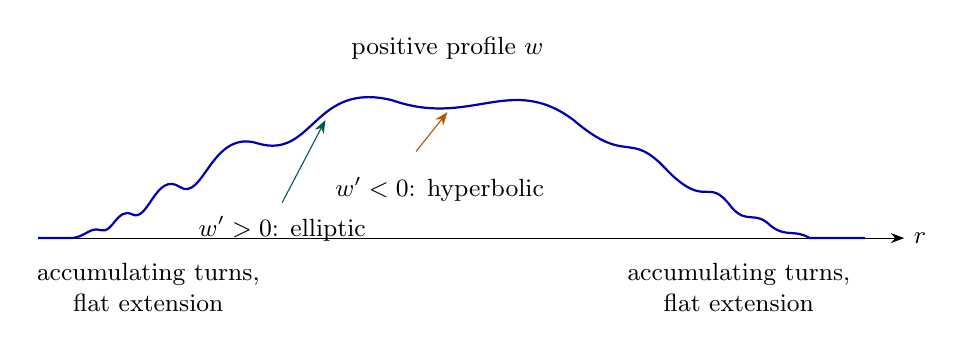
\begin{tikzpicture}[x=1cm,y=1cm,>=Stealth,font=\small]
\draw[->] (0,0)--(11,0) node[right] {$r$};
\draw[thick,blue!70!black] (0,0)--(.4,0)
 .. controls (.6,0) and (.65,.15) .. (.8,.1)
 .. controls (.95,.05) and (1,.4) .. (1.2,.3)
 .. controls (1.4,.2) and (1.5,.85) .. (1.8,.65)
 .. controls (2.1,.45) and (2.2,1.4) .. (2.8,1.2)
 .. controls (3.5,1) and (3.5,2) .. (4.5,1.75)
 .. controls (5.5,1.4) and (6,2.1) .. (6.8,1.5)
 .. controls (7.5,.9) and (7.5,1.4) .. (8.0,.85)
 .. controls (8.5,.35) and (8.5,.8) .. (8.8,.4)
 .. controls (9.0,.16) and (9.1,.36) .. (9.3,.16)
 .. controls (9.5,0) and (9.6,.12) .. (9.8,0)--(10.5,0);
\node[above] at (5.2,2.15) {positive profile $w$};
\node[below,align=center] at (1.4,-.2) {accumulating turns,\\flat extension};
\node[below,align=center] at (8.9,-.2) {accumulating turns,\\flat extension};
\draw[->,orange!70!black] (4.8,1.1)--(5.2,1.6);
\node[below] at (5.1,.9) {$w'<0$: hyperbolic};
\draw[->,teal!70!black] (3.1,.45)--(3.65,1.5);
\node[below] at (3.1,.4) {$w'>0$: elliptic};
\end{tikzpicture}
\caption{The shape of an admissible profile. Only a few representative
turns are drawn, and not to scale. Where $w$ rises the linearized
equation is elliptic, where it falls it is hyperbolic. Every derivative
of $w$ tends to zero at the two accumulation points.}
\label{fig:profile-type}
\end{figure}

\subsection{Two resonance conditions in a finite model}
\label{sec:worked-example}

Before constructing the profile we examine a model with exactly two
turning circles, in which everything can be computed. It is a guide to
the construction of Part~\ref{part:reference} and is not used in any
proof. Its purpose is to show that an inverse of $\mathscr L_w$
involves two different sets of small denominators.

\paragraph{The model.}
Put $\epsilon=\sqrt2/100$ and $\rho(X)=\epsilon^2X(1-X)$, and let
$r(X)$ solve, on $-1\le X\le2$,
\begin{equation}\label{eq:example-radius}
 r_{XX}=-\rho\,r,\qquad r(0)=1,\qquad r_X(0)=\frac1{10}.
\end{equation}
On this interval $|\rho|\le2\epsilon^2$, so the integral form of
\eqref{eq:example-radius} bounds $R=\max|r|$ by
$R\le1.2+4\epsilon^2R$. Hence $R<1.21$, $r>0.89$ and
$|r_X-\tfrac1{10}|\le4\epsilon^2R<0.001$. In particular $r$ is
increasing, and we may define a positive profile by
\[
 w(r(X))=r_X(X).
\]
Then $w'=dw/dr=-\rho\,r/r_X$, so $w$ has exactly two turning circles,
at $X=0$ and $X=1$, and the equation is hyperbolic between them. For an
angular mode $u=U(X)\cos(j\theta)$ the operator
\eqref{eq:intro-linearization} becomes, with $J=j\epsilon$,
\begin{equation}\label{eq:example-mode}
 L_jU=\frac1{r_X}\bigl(U_{XX}+J^2X(1-X)\,U\bigr).
\end{equation}

\paragraph{First denominator: characteristics.}
On $0<X<1$ the characteristics of $\mathscr L_w$ have slopes
$d\theta/dX=\pm\epsilon\sqrt{X(1-X)}$. Between the two turning circles
each of them turns by the \emph{travel angle}
\begin{equation}\label{eq:example-action}
 T=\epsilon\int_0^1\sqrt{X(1-X)}\,dX=\frac{\epsilon\pi}8 .
\end{equation}
The two families of characteristics translate a function on the circle
by $+T$ and by $-T$, and reconciling them requires inverting the
difference of the two translations,
\begin{equation}\label{eq:example-circle-operator}
 \mathcal D_Tf(\theta)=f(\theta+T)-f(\theta-T),\qquad
 \mathcal D_T\sin(j\theta)=2\sin(jT)\cos(j\theta).
\end{equation}
So the characteristic problem costs the divisor $\sin(jT)$. Here
$jT/\pi=j\sqrt2/800$ is a quadratic irrational multiple of $j$. If $m$
is the integer nearest to $j\sqrt2/800$, the integer
$2j^2-640000\,m^2$ is nonzero; factoring it, and using
$j\sqrt2/800+|m|\le j$ and $|\sin(\pi x)|\ge2\dist(x,\Z)$, we obtain
\begin{equation}\label{eq:example-diophantine-bound}
 |\sin(jT)|\ge\frac1{320000\,j}\qquad(j\ge1).
\end{equation}
The inverse of $\mathcal D_T$ exists on functions of mean zero and
loses one angular derivative. No choice of $T$ avoids a loss
altogether. If $T/\pi$ is rational, $\sin(jT)=0$ for infinitely many
even $j$. If it is irrational, apply the pigeonhole principle to the
fractional parts of $2kT/\pi$, $0\le k\le N$: two of them differ by
at most $1/N$, which gives an even $j\le2N$ with
$|\sin(jT)|\le\pi/N$. So the divisors are never bounded below, and
a bound like \eqref{eq:example-diophantine-bound} is the best one
can ask for.

\paragraph{Second denominator: matching.}
Now consider the boundary value problem for \eqref{eq:example-mode}.
The substitution $x=\sqrt J\,(X-\tfrac12)$ turns the homogeneous
equation into the harmonic oscillator equation
\begin{equation}\label{eq:example-oscillator}
 (-\partial_x^2+x^2)\,U=\frac J4\,U .
\end{equation}
As boundary condition at each end of the interval we require that
$(U,U_X)$ be proportional to the data of the solution of
\eqref{eq:example-oscillator} on the whole line which decays in that
direction. These are legitimate boundary conditions for
\eqref{eq:example-mode}; the radius need not be extended beyond
$[-1,2]$. The homogeneous problem then has a nonzero solution exactly
when one solution decays in both directions, that is, when $J/4$ is an
eigenvalue of the oscillator. The eigenvalues are the odd integers
$2m+1$ \cite[Section~8.3]{Teschl2009}, so the resonances are
\begin{equation}\label{eq:example-spectral-phase}
 \frac J4=2m+1,
 \qquad\text{equivalently}\qquad
 jT=\bigl(m+\tfrac12\bigr)\pi .
\end{equation}
Away from them the inhomogeneous problem is solved by the resolvent of
the oscillator: multiply the source by $-r_X/J$, extend it by zero
outside $|x|\le3\sqrt J/2$, apply the resolvent on the whole line, and
restrict. Thus the boundary value problem has precisely the
denominators \eqref{eq:example-spectral-phase}; this is an exact
statement, not a comparison of formal phases.

\begin{figure}[htbp]
\centering
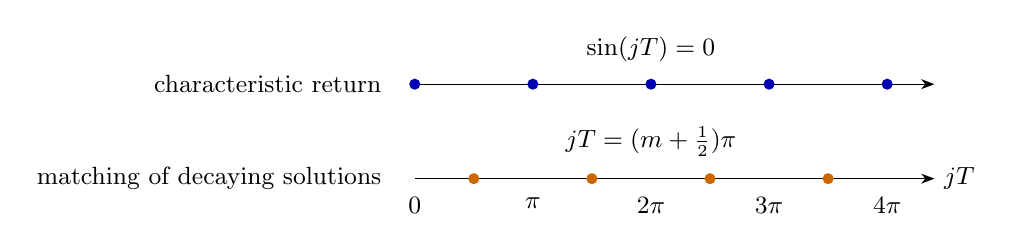
\begin{tikzpicture}[x=1.5cm,y=.8cm,>=Stealth,font=\small]
\node[anchor=east] at (-.2,1.5) {characteristic return};
\node[anchor=east] at (-.2,0) {matching of decaying solutions};
\draw[->] (0,1.5)--(4.4,1.5);
\draw[->] (0,0)--(4.4,0) node[right] {$jT$};
\foreach \x/\t in {0/0,1/\pi,2/2\pi,3/3\pi,4/4\pi}{
 \fill[blue!70!black] (\x,1.5) circle (2pt);
 \node[below] at (\x,-.15) {$\t$};}
\foreach \x in {.5,1.5,2.5,3.5}{
 \fill[orange!80!black] (\x,0) circle (2pt);}
\node[above] at (2,1.7) {$\sin(jT)=0$};
\node[above] at (2,.2) {$jT=(m+\tfrac12)\pi$};
\end{tikzpicture}
\caption{The two resonance sets of the finite model, as functions of
the phase $jT$. Avoiding one row does not avoid the other. In the
infinite construction both must be kept at a controlled distance.}
\label{fig:two-denominators}
\end{figure}

\paragraph{Remark on the half-integer shift.}
The shift by $\pi/2$ between the two rows of
Figure~\ref{fig:two-denominators} has a local explanation. Near $X=0$
put $y=J^{2/3}X$; then
\[
 U_{yy}+yU=J^{-2/3}y^2\,U .
\]
On a fixed $y$-interval the solutions are, up to an error
$O(J^{-2/3})$ in value and first derivative, combinations of the Airy
functions $\Ai(-y)$ and $\Bi(-y)$; this follows by variation of
constants and Gronwall's inequality. The asymptotics of the Airy
functions carry a phase shift $\pi/4$ at each turning point
\cite[9.7.5--9.7.12]{DLMFAiry}, and two turning points give $\pi/2$.
This is only a heuristic; \eqref{eq:example-spectral-phase} was proved
by the exact oscillator computation.

\paragraph{What the model teaches.}
In the actual construction the travel angle of every hyperbolic
annulus will be a quadratic irrational multiple of $\pi$, which gives
a bound of the type \eqref{eq:example-diophantine-bound}; and the
matching problem, now between infinitely many pieces, will be
controlled by spectral gaps of the individual pieces together with a
choice of their relative heights.

\subsection{Normalization and the conservation law}
\label{subsec:normalization}

The nonlinear unknown is $z=h+qu$ with a small parameter $q$. Since
$\mathcal N_h(h)=0$, the residual of $z$ is divisible by $q$, and we
define the \emph{normalized residual}
\begin{equation}\label{eq:cart-removable-equation}
 \mathcal F_q(w,u)=
 \begin{cases}r\,\mathcal N_h(h+qu)/q,&q\ne0,\\[2pt]
 \mathscr L_wu,&q=0.
 \end{cases}
\end{equation}
It is smooth in $q$ through $q=0$, because
\begin{equation}\label{eq:normalized-integral}
 \mathcal F_q(w,u)=\int_0^1 r\,D_z\mathcal N_h(h+tqu)\,u\,dt .
\end{equation}
It depends on $h$ only through $w$, and it does not change when a
constant is added to $u$.

\paragraph{Symmetry class.}
From now on all heights are even in $\theta$ and invariant under
$\theta\mapsto\theta+\pi$. This class is preserved by products and by
$\mathcal F_q$. Its Fourier modes are $\cos(j\theta)$ with $j\ge0$
even.

\begin{lemma}[Conservation law]\label{lem:scalar-integral}
Let $w$ be flat at both endpoints and let $u$ have constant
extensions at both endpoints, with $D>0$ for $z=h+qu$. Then
\begin{equation}\label{eq:zero-total-integral}
 \int_{r_-}^{r_+}\av{\mathcal F_q(w,u)}\,dr=0 .
\end{equation}
The same holds for every derivative of $\mathcal F_q(w,u)$ with
respect to $u$, $q$ or $w$ in directions preserving these conditions.
\end{lemma}

\begin{proof}
By Proposition~\ref{prop:scalar-core}(ii) and Stokes' theorem,
$\int\!\!\int r\mathcal N_h(z)\,dr\,d\theta$ is the difference of the
periods $\oint\alpha$ over the two boundary circles. At a boundary
circle $w=0$ and $dz=0$ to infinite order, so $D=1$ and
$\alpha=d\theta$ there: both periods equal $2\pi$. Differentiating the
identity gives the last statement.
\end{proof}

\paragraph{The connection period.}
The angular mean of the equation is most transparent at the level of
the connection form. For a height $z=h+U$ define
\begin{equation}\label{eq:cart-mean-path-flux}
 \mathfrak F_w(U)=\av{\alpha_\theta}-1
 =\left\langle\frac{1+kp_\theta/(1-p^2)}{\sqrt D}\right\rangle-1,
\end{equation}
the normalized period of $\alpha$ over the circle of radius $r$. Since
$\partial_r\alpha_\theta-\partial_\theta\alpha_r=r\mathcal N_h$, its
radial derivative is $r\av{\mathcal N_h(h+U)}$, and it vanishes at the
endpoints. So the mean of the equation $\mathcal N_h(h+U)=0$ is
equivalent to
\[
 \mathfrak F_w(U)=0\qquad\text{for all }r .
\]
Formula~\eqref{eq:conn-exact-variation} gives the derivative of
$\mathfrak F_w$ with respect to a radial variation $\bar U(r)$ of the
height, and its full derivative at $U=0$:
\begin{equation}\label{eq:mean-period-derivative}
 \partial_{\bar U'}\mathfrak F_w(U)=\av a,
 \qquad D_U\mathfrak F_w(0)[U]=w\av{U_r}.
\end{equation}
The second formula says that, to first order, the period sees only the
mean of the height. This cancellation is the reason why the mean of
the solution will decay twice as fast as its oscillating part
(Section~\ref{sec:final-proof}).

\subsection{The first residual correction}
\label{subsec:first-correction}

By \eqref{eq:cart-determinant-identity}, the type of the true
linearization \eqref{eq:cart-true-derivative} is governed by
$K_0/D^2+ED^{-3/2}\mathcal N_h(z)$. At a solution the second term
vanishes and the type changes exactly where $w'$ does. Away from a
solution the second term moves the turning circles, which is
inconvenient: the circles would depend on the unknown. We remove that
term by changing the tangential coefficient $c$ only.

\begin{lemma}[Fixing the type-change set]\label{lem:type-completion}
On the set of heights with $D\ge\tfrac12$ and $Q\ge\tfrac78w>0$ put
\[
 B=\frac{E}{rQ},\qquad \bar c=c-B\,r\,\mathcal N_h(z),\qquad
 \bar L=\partial_r(a\partial_r+b\partial_\theta)
             +\partial_\theta(b\partial_r+\bar c\,\partial_\theta).
\]
Then
\begin{equation}\label{eq:cart-completed-normalized-derivative}
 a\bar c-b^2=\frac{K_0}{D^2},\qquad
 D_u\mathcal F_q(w,u)\,\eta=\bar L\eta
       +q\,\partial_\theta\bigl(B\,\mathcal A\,\eta_\theta\bigr),
 \qquad \mathcal A=\mathcal F_q(w,u),
\end{equation}
where $\bar L$ is formed with the coefficients of $z=h+qu$. The
operator $\bar L$ is symmetric for $dr\,d\theta$, annihilates
constants, and has the same normal flux $a\eta_r+b\eta_\theta$ as the
true derivative.
\end{lemma}

\begin{proof}
The determinant changes by $-aB\,r\mathcal N_h=-ED^{-3/2}\mathcal N_h$,
which cancels the unwanted term of
\eqref{eq:cart-determinant-identity}. The operator changes by
$-\partial_\theta(B\,r\mathcal N_h\,\partial_\theta)$, and
$r\mathcal N_h(h+qu)=q\mathcal A$. Only the tangential coefficient was
modified, which gives the remaining assertions.
\end{proof}

Thus $\bar L$ is elliptic exactly where $w'>0$ and hyperbolic exactly
where $w'<0$, whatever the height. The price is the term
$q\,\partial_\theta(B\mathcal A\eta_\theta)$, which is the product of
the residual $\mathcal A$ and the increment $\eta$. An error of this
bilinear form is exactly what Hamilton's version of the implicit
function theorem tolerates (Section~\ref{sec:solving-the-equation}).
This is the first residual correction. The second, which fixes the
characteristic return maps, is made in
Section~\ref{sec:fixed-geometry}.

\paragraph{Characteristics.}
For later reference we record the characteristic directions of
$\bar L$ on a component of $\{w'<0\}$:
\begin{equation}\label{eq:completed-characteristics}
 \frac{d\theta}{dr}=d\pm v,\qquad
 d=\frac ba=\frac{E(p-k_\theta)}{rQ},\qquad
 v=\frac{\sqrt{b^2-a\bar c}}{a}
  =\frac{\sqrt{-ww'/r}\,\sqrt D}{Q}.
\end{equation}
We call $v$ the \emph{characteristic speed}. At the radial height
$d=0$ and $v=\sqrt{-w'/(rw)}$. At a turning circle $v$ is a smooth
positive factor times the square root of the distance into the
hyperbolic side. The coordinates of
Section~\ref{sec:fixed-geometry} are built to respect this
degeneracy; treating all intervals as uniformly elliptic or uniformly
hyperbolic would lose the geometry of the problem.


\part{The reference profile}
\label{part:reference}
\section{The reference profile: requirements and solvable models}
\label{sec:rosen-reference-packet}
\label{sec:radial-models}

Part~\ref{part:reference} constructs one radial profile $w_*$ at which
the linearized equation has a single flat infinitesimal bending and a
controlled inverse. This section states precisely what is needed
(Proposition~\ref{prop:rad-fixed-theorem}), explains the layout of the
construction and its vocabulary, and introduces the two explicitly
solvable models from which $w_*$ is assembled.

\subsection{Angular modes and the design problem}

Functions in our symmetry class have the Fourier expansion
\[
 u(r,\theta)=u_0(r)+\sum_{\substack{j\ge2\\ j\ \mathrm{even}}}
 u_j(r)\,e_j(\theta),
 \qquad e_j(\theta)=\sqrt2\cos(j\theta),
\]
and on the $j$th mode the operator \eqref{eq:intro-linearization} acts
as the ordinary differential operator
\begin{equation}\label{eq:rad-eq-modal-operator}
 L_ju=(wu')'-j^2\,\frac{w'}r\,u,
 \qquad\text{that is,}\qquad
 \mathscr L_w(u\,e_j)=(L_ju)\,e_j .
\end{equation}
When the dependence on the profile matters we write $L_{j,w}$. We want
a profile for which
\begin{itemize}
\item at $j=2$ there is exactly one solution of $L_2\phi=0$, up to
 multiples, which is flat at both endpoints. This is the seed of the
 nonradial height. The frequency two is the lowest one compatible with
 the half-turn symmetry required in
 Theorem~\ref{thm:geometric-closure};
\item at every even $j\ge4$ there is no such solution, and $L_j$ has a
 controlled inverse. The nonlinear equation creates all higher even
 frequencies, so all of them must be invertible on the same profile.
\end{itemize}

Two freedoms are available, and separating them is the organizing idea
of the construction. The \emph{shape} of a piece of the profile
determines the homogeneous solutions on that piece, hence its spectrum
and its travel angles. Multiplying a piece by a positive constant, its
\emph{height}, changes none of these, but it changes the scale of the
flux $wu'$ by which solutions on neighbouring pieces are compared. We
use the first freedom to make each piece explicitly solvable, and the
second to prevent resonances when the pieces are joined.

\subsection{What the reference profile must provide}
\label{sec:radial-what}

We state the result of Part~\ref{part:reference} before starting the
construction. It involves three scales attached to the $n$th piece of
the profile near an endpoint.

\begin{definition}[The endpoint scales]\label{def:radial-weights}
The pieces of the profile approaching either endpoint are called
\emph{cells} and are indexed by integers $n\ge N$. We set
\begin{equation}\label{eq:rad-eq-endpoint-weights}
 A_n\asymp e^{-n^2},\qquad
 S_n=\tfrac23\,n^3,\quad H_n=e^{-S_n},\qquad
 q_n=n^{5/2}\log(e+n),\quad \mathcal E_n=e^{q_n}.
\end{equation}
\begin{itemize}
\item $A_n$ is the \emph{length scale}: cell $n$ has radial length
 comparable to $A_n$.
\item $H_n$ is the \emph{decay scale}: the distinguished solution of
 $L_j u=0$ at the endpoint decays like $H_n$ across the cells.
\item $\mathcal E_n$ is the \emph{coefficient allowance}: reciprocals
 and derivatives of the coefficients on cell $n$ are bounded by powers
 of $\mathcal E_n$.
\end{itemize}
A bound of the form $C\mathcal E_n^{C}$ is called a \emph{coefficient
power}; a \emph{coefficient estimate of order $s$} on cell $n$ is a
bound by $C_s\mathcal E_n^{C_s}$. On the finitely many pieces in the
middle of the annulus the same words refer to fixed positive
constants. For the purpose of estimates a cell includes fixed portions
of its neighbours; such an enlargement changes the index by a bounded
amount, which is immaterial.
\end{definition}

The three scales are ordered: for all fixed $a,b,\varepsilon>0$,
\begin{equation}\label{eq:rad-scale-separation}
 \mathcal E_n^{a}\,e^{bn^2}\le C_{a,b,\varepsilon}\,e^{\varepsilon S_n},
 \qquad\text{because}\qquad n^2=o(q_n),\quad q_n=o(S_n).
\end{equation}
So lengths are much larger than coefficient allowances, which are much
larger than the decay scale. Section~\ref{sec:radial-tails} derives all
three scales from the construction; they are not hypotheses about an
unknown profile.

\paragraph{Weighted norms.}
Choose a smooth partition of unity $\vartheta_m$ on $(r_-,r_+)$ with
bounded overlap, subordinate to the cells of both tails and to the
finite middle part; the index $m$ records both the endpoint and the
cell. Fix a smooth function $\chi_L$ of $r$ equal to one near the left
endpoint and to zero near the right one. For exponents $0<\gamma<1$
and $\ea\ge0$, the \emph{source norm} of a pair $(f,c)$, consisting of
a function $f$ and a scalar $c$, is
\begin{equation}\label{eq:rad-eq-source-norm}
 \|(f,c)\|_{Y_{\gamma,s}}^2
 =|c|^2+\sum_m\mathcal E_m^{2\ea}H_m^{-2\gamma}
       \|\vartheta_m f\|_{L^2(dr)H^s(\T)}^2 .
\end{equation}
The \emph{output norm} is defined for pairs $(u,\nu)$ of a function
and a scalar. Write $u=a_L\chi_L+v$ with a constant $a_L$; then the
squared output norm is
\[
 |a_L|^2+|\nu|^2+\sum_m\mathcal E_m^{-2\eb}H_m^{-2\gamma}
       \|\vartheta_m v\|_{L^2(dr\,d\theta)}^2 .
\]
A finite source norm means decay like $H_m^{\gamma}$ towards the
endpoints, with $\ea$ powers of the coefficient allowance to spare. A
finite output norm means the same decay for $v$, after the loss of
$\ea+\eb$ such powers, while $u$ itself tends to $a_L$ at the left
endpoint and to $0$ at the right one.

\begin{proposition}[The reference profile]\label{prop:rad-fixed-theorem}
There are radii $0<r_-<r_+$ and a smooth function $w_*>0$ on
$(r_-,r_+)$, flat at both endpoints, such that all zeros of $w_*'$ in
$(r_-,r_+)$ are simple, with the following properties.
\begin{enumerate}
\item \textup{(Kernel.)} There is a nonzero function $\phi_*$, flat at
 both endpoints, with $L_{2,w_*}\phi_*=0$. It spans the endpoint-flat
 kernel of $L_{2,w_*}$, and the endpoint-flat kernel of $L_{j,w_*}$ is
 zero for every even $j\ge4$.
\item \textup{(Travel angles.)} For every component $m$ of
 $\{w_*'<0\}$ the travel angle
 $T_m=\int\sqrt{-w_*'/(rw_*)}\,dr$ over that component satisfies
 \begin{equation}\label{eq:rad-eq-optical-margin}
  |\sin(kT_m)|\ge\frac{\gamma_m}{k}\quad(k\ge1),
  \qquad \gamma_m^{-1}\le\mathcal E_m^{C},
  \qquad T_m/\pi\ \text{is a quadratic irrational}.
 \end{equation}
\item \textup{(Border.)} There is a smooth function $\chi_*$,
 compactly supported in a component of $\{w_*'>0\}$, such that
 \begin{equation}\label{eq:rad-eq-target-border}
  g_*=L'_{2,w_*}[w_*\chi_*]\,\phi_*,\qquad
  \int g_*\phi_*\,dr=1,\qquad
  \ell_*u=\int g_*u_2\,dr .
 \end{equation}
 Here $L'_{2,w}[\omega]\phi=(\omega\phi')'-4\omega'\phi/r$ is the
 derivative of $L_{2,w}\phi$ with respect to the profile $w$ in the
 direction $\omega$.
\item \textup{(Inverse.)} The bordered operator
 \begin{equation}\label{eq:rad-eq-bordered-reference}
  \mathbb L_{w_*}(u,\nu)
    =\bigl(\mathscr L_{w_*}u+\nu\,g_*e_2,\ \ell_*u\bigr)
 \end{equation}
 has a two-sided inverse on the sources $(f,c)$ satisfying the
 compatibility condition $\int\av f\,dr=0$, where $u$ is required to
 tend to zero at the right endpoint and to an arbitrary constant at
 the left one. For every compact interval
 $[\gamma_-,\gamma_+]\subset(0,1)$ there are exponents $\ea,\eb$ such
 that this inverse is bounded from $Y_{\gamma,0}$ to the output norm,
 uniformly for $\gamma\in[\gamma_-,\gamma_+]$. One radial derivative
 of the output costs at most one additional angular derivative of the
 source.
\item \textup{(Independence of the exponent.)} The profile, the
 function $\phi_*$ and the border are the same for all exponents
 $\gamma$.
\end{enumerate}
\end{proposition}

Some comments on the statement.

\emph{The border.} Since $L_2$ has a one-dimensional kernel, and is
formally symmetric, it has a one-dimensional cokernel as well. The
standard remedy is to \emph{border} the operator: one adds a scalar
unknown $\nu$ multiplying a fixed function $g_*$ (the \emph{column})
and a scalar equation $\ell_*u=c$ (the \emph{row}). The column removes
the cokernel and the row removes the kernel. Our column has a
meaning: if the profile is deformed to $w_*e^{\nu\chi_*}$, then
$g_*e_2$ is the derivative of
$\mathscr L_w(\phi_*e_2)$ with respect to $\nu$. So $\nu$ will be an
actual parameter of the metric in the nonlinear problem.

\emph{The compatibility condition and the free constant.} These
concern the mode $j=0$, where $L_0u=(wu')'$. By
Lemma~\ref{lem:scalar-integral} the sources of interest have
$\int\av f\,dr=0$; and the difference of the two endpoint values of
the height is not prescribed.

\emph{Endpoint-flat kernel.} The precise meaning of this term, and of
the two-sided inverse, is given by the weighted graph domain of
Definition~\ref{def:radial-graph-domain}.

\emph{What is proved here, and what later.}
Proposition~\ref{prop:rad-fixed-theorem} is an estimate at angular
order zero, together with its first radial derivative. Estimates of
all orders are recovered from the differential equation in
Section~\ref{sec:stable-inverse}, after the weighted spaces of the
nonlinear problem have been introduced. Keeping the two tasks apart
means that the geometry of the profile does not depend on the order
of regularity.

The proof of Proposition~\ref{prop:rad-fixed-theorem} occupies the
rest of this section and the next two; it is completed in
Section~\ref{subsec:final-border}.

\subsection{Layout of the construction and vocabulary}
\label{subsec:layout}

Figure~\ref{fig:layout} shows how $w_*$ is assembled. The following
terms are used throughout Parts~\ref{part:reference}
and~\ref{part:nonlinear}.

\begin{figure}[htbp]
\centering
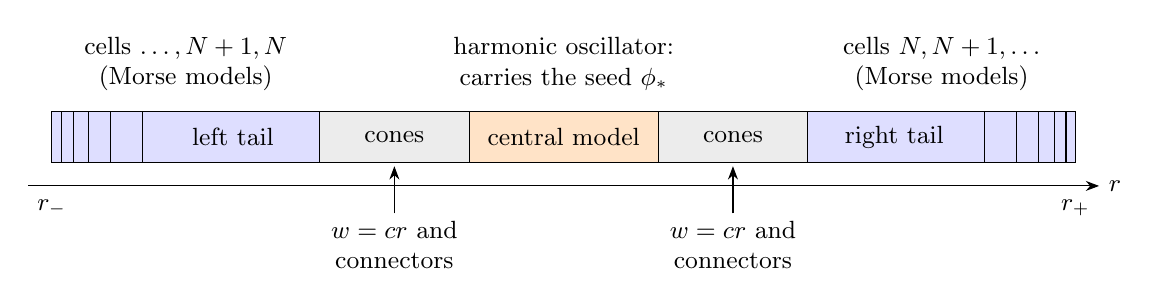
\begin{tikzpicture}[x=1cm,y=1cm,>=Stealth,font=\small]
\draw[->] (-.3,0)--(13.3,0) node[right] {$r$};
\draw[fill=blue!13] (0,.3) rectangle (3.4,.95);
\draw[fill=gray!15] (3.4,.3) rectangle (5.3,.95);
\draw[fill=orange!22] (5.3,.3) rectangle (7.7,.95);
\draw[fill=gray!15] (7.7,.3) rectangle (9.6,.95);
\draw[fill=blue!13] (9.6,.3) rectangle (13,.95);
\node at (2.3,.62) {left tail};
\node at (4.35,.62) {cones};
\node at (6.5,.62) {central model};
\node at (8.65,.62) {cones};
\node at (10.7,.62) {right tail};
\foreach \x in {.12,.27,.47,.75,1.15}{\draw (\x,.3)--(\x,.95);}
\foreach \x in {12.88,12.73,12.53,12.25,11.85}{\draw (\x,.3)--(\x,.95);}
\node[below] at (0,-.05) {$r_-$};
\node[below] at (13,-.05) {$r_+$};
\node[align=center] at (1.7,1.55) {cells $\ldots,N+1,N$\\(Morse models)};
\node[align=center] at (11.3,1.55) {cells $N,N+1,\ldots$\\(Morse models)};
\node[align=center] at (6.5,1.55) {harmonic oscillator:\\carries the seed $\phi_*$};
\node[align=center] at (4.35,-.75) {$w=cr$ and\\connectors};
\node[align=center] at (8.65,-.75) {$w=cr$ and\\connectors};
\draw[->] (4.35,-.35)--(4.35,.25);
\draw[->] (8.65,-.35)--(8.65,.25);
\end{tikzpicture}
\caption{The layout of the reference profile $w_*$ (schematic). The
cells shrink and accumulate at both endpoints. Consecutive pieces are
separated by intervals on which $w_*'>0$.}
\label{fig:layout}
\end{figure}

\begin{description}[leftmargin=1.5em,style=sameline,font=\normalfont\itshape]
\item[Positive and negative components.] A \emph{positive component}
 is a component of $\{w'>0\}$; the equation is elliptic there. A
 \emph{negative component} is a component of $\{w'<0\}$; the equation
 is hyperbolic there. They are separated by the turning circles, also
 called \emph{roots}.
\item[Travel angle.] The travel angle of a negative component is
 $T=\int\sqrt{-w'/(rw)}\,dr$ over that component: the angle by which a
 characteristic of $\mathscr L_w$ turns while crossing it.
\item[Model.] A piece of the profile on which, in a suitable
 \emph{model coordinate} $X$, every $L_j$ is conjugate to an
 explicitly solvable Schr\"odinger operator
 (Section~\ref{subsec:liouville}). There are two kinds: the
 \emph{central model} and the Morse \emph{cells}.
\item[Cell.] The $n$th cell consists, in the direction of increasing
 $r$, of a \emph{short positive cap}, one negative component, and a
 \emph{long positive cap} (Figure~\ref{fig:cell}).
\item[Join.] A very short positive interval between two consecutive
 cells, on which $w$ rises steeply from the height of one cell to that
 of the next.
\item[Cone.] An interval on which $w=cr$. There
 $L_ju=c\,[(ru')'-j^2u/r]$ has the solutions $r^{\pm j}$.
\item[Connector.] A positive interval joining the central model or a
 tail to a cone, built so that the seed solution is preserved exactly
 (Section~\ref{subsec:rad-cone-bump-target-match}).
\item[Tail.] The union of the cells and joins near one endpoint.
\item[Buffer.] A positive interval, viewed as a region across which
 the solutions of $L_ju=0$ grow or decay exponentially; it decouples
 the pieces on its two sides.
\item[Natural line, incoming line.] At a point of a tail, and for a
 fixed frequency $j$, the \emph{natural line} is the one-dimensional
 space of solutions of $L_ju=0$ that decay towards the endpoint
 (Lemma~\ref{lem:radial-deep-inverse}). The \emph{incoming line} is
 the one-dimensional space of solutions satisfying the condition
 imposed on the interior side. A homogeneous solution of the whole
 problem exists exactly when the two lines coincide.
\item[Outward.] Towards the nearer endpoint.
\end{description}

The plan of Part~\ref{part:reference} is as follows.
\begin{itemize}
\item Section~\ref{subsec:liouville} explains how a Schr\"odinger
 potential determines a radial profile.
 Sections~\ref{subsec:rad-central-singlepoint}
 and~\ref{subsec:morse} treat the central model and the Morse model on
 the whole line: spectrum, spectral gap at energy zero, travel angle.
\item Section~\ref{sec:radial-tails} builds the tails. It proves that
 at every frequency the natural line exists, is unique, and consists
 of flat functions, and it chooses the heights of the cells so that
 natural and incoming lines stay apart.
\item Section~\ref{sec:radial-reference-inverse} joins all pieces and
 proves that the local information combines to an inverse on the whole
 annulus.
\end{itemize}

\subsection{From a Schr\"odinger potential to a radial profile}
\label{subsec:liouville}

It is easier to design the spectrum first and the radius afterwards.

\begin{lemma}[Liouville transformation]\label{lem:liouville}
Let $X$ range over an interval, let $r(X)$ be a smooth function with
$r>0$ and $r_X>0$, let $\mathcal P(X)>0$ be smooth, and let
$\lambda>0$. Define a profile $w$ and two functions $\rho,V_0$ of $X$
by
\begin{equation}\label{eq:rad-eq-sc0}
 w(r(X))=\lambda\,\mathcal P(X)\,r_X(X),\qquad
 \rho=-\frac{r_{XX}+(\mathcal P_X/\mathcal P)\,r_X}{r},\qquad
 V_0=\frac{(\sqrt{\mathcal P})_{XX}}{\sqrt{\mathcal P}} .
\end{equation}
Then $w'=-\lambda\mathcal P\rho\,r/r_X$, and for every $j$ and every
function $\psi(X)$,
\begin{equation}\label{eq:liouville-identity}
 L_j\bigl(\mathcal P^{-1/2}\psi\bigr)
   =-\frac{\lambda\sqrt{\mathcal P}}{r_X}\,
      \bigl(-\psi_{XX}+(V_0-j^2\rho)\,\psi\bigr).
\end{equation}
\end{lemma}

\begin{proof}
For a function $u$ of $r$ we have $wu_r=\lambda\mathcal Pu_X$, hence
$(wu_r)_r=\lambda(\mathcal Pu_X)_X/r_X$. Differentiating
$w=\lambda\mathcal Pr_X$ and using the definition of $\rho$ gives the
formula for $w'$. Therefore
$L_ju=(\lambda/r_X)\,[(\mathcal Pu_X)_X+j^2\mathcal P\rho\,u]$, and
with $u=\mathcal P^{-1/2}\psi$ one has
$(\mathcal Pu_X)_X=\sqrt{\mathcal P}\,(\psi_{XX}-V_0\psi)$.
\end{proof}

We use the lemma in the opposite direction. Given a density
$\mathcal P$ and a function $\rho$, the homogeneous equation
$L_ju=0$ is equivalent to the Schr\"odinger equation
\[
 H_j\psi:=-\psi_{XX}+(V_0-j^2\rho)\,\psi=0 ,
\]
\emph{provided} the linear equation
$r_{XX}+(\mathcal P_X/\mathcal P)\,r_X+\rho\,r=0$ for the radius has a
solution which is positive and increasing. Three features of the
dictionary are used constantly.
\begin{itemize}
\item The height $\lambda$ does not enter the homogeneous equation.
\item The profile is falling where $\rho>0$ and rising where $\rho<0$.
 The negative components are the components of $\{\rho>0\}$, the
 turning circles are the zeros of $\rho$, and the travel angle of a
 negative component is
 \begin{equation}\label{eq:travel-angle-model}
  T=\int\sqrt{-w'/(rw)}\,dr=\int_{\{\rho>0\}}\sqrt\rho\,dX .
 \end{equation}
\item Frequency enters only through the coupling constant $j^2$ in
 front of $\rho$.
\end{itemize}

We use two potentials with complementary roles
(Figure~\ref{fig:two-spectral-models}). The harmonic oscillator, in
the middle, has a zero mode at $j=2$ and is used to create the seed.
The Morse potential, near the ends, has a spectral gap at energy zero
for all $j$, and its cells are short enough in radius to accumulate at
a finite point. It is the explicit spectra of the two models, not
merely the shapes of their potentials, that make them useful.

\begin{figure}[htbp]
\centering
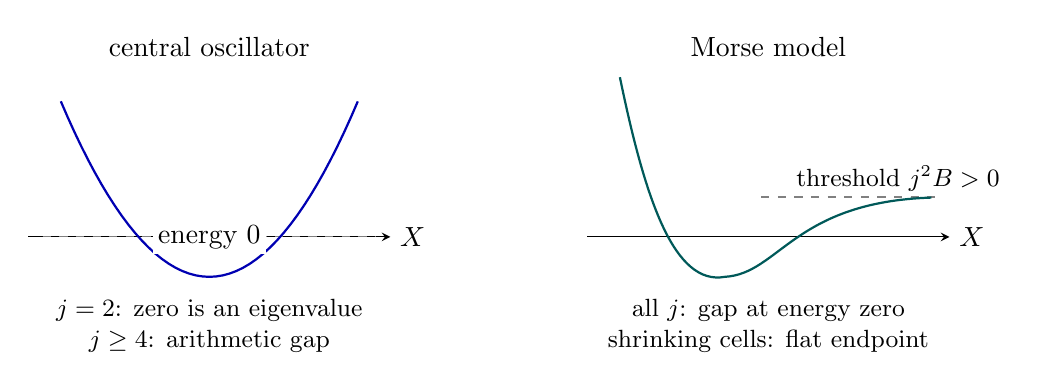
\begin{tikzpicture}[x=.92cm,y=.78cm,>=stealth]
\begin{scope}
\draw[->] (-2.5,0)--(2.5,0) node[right] {$X$};
\draw[dashed,gray] (-2.3,0)--(2.3,0);
\draw[thick,blue!70!black,domain=-2.05:2.05,samples=45]
 plot (\x,{.68*\x*\x-.65});
\node[align=center] at (0,3.1) {central oscillator};
\node[fill=white,inner sep=2pt] at (0,0) {energy $0$};
\node[align=center,font=\small] at (0,-1.45)
 {$j=2$: zero is an eigenvalue\\$j\ge4$: arithmetic gap};
\end{scope}
\begin{scope}[xshift=7.1cm]
\draw[->] (-2.5,0)--(2.5,0) node[right] {$X$};
\draw[dashed,gray] (-.1,.65)--(2.3,.65);
\draw[thick,teal!70!black]
 (-2.05,2.6) .. controls (-1.7,.6) and (-1.3,-.8) .. (-.6,-.65)
 .. controls (.15,-.6) and (.35,.57) .. (2.25,.64);
\node[align=center] at (0,3.1) {Morse model};
\node[anchor=west,font=\small] at (.25,.95) {threshold $j^2B>0$};
\node[align=center,font=\small] at (0,-1.45)
 {all $j$: gap at energy zero\\shrinking cells: flat endpoint};
\end{scope}
\end{tikzpicture}
\caption{The potentials $V_0-j^2\rho$ of the two models on the whole
line, drawn schematically with an arbitrary vertical scale. Only
finite pieces of them are used in the profile, and the pieces are
separated by regions where the potential is positive.}
\label{fig:two-spectral-models}
\end{figure}

\subsection{The central oscillator}
\label{subsec:rad-central-singlepoint}

\paragraph{Definition and spectrum.}
Fix the constants
\begin{equation}\label{eq:rad-eq-sc1}
 A_c=\frac1{\sqrt2},\qquad a_c=\sqrt{4A_c-2},\qquad
 c_c=3A_c-2>0,\qquad \alpha_c=\frac{c_c+1}2,
\end{equation}
and take
\[
 \mathcal P=e^{-2a_cX},\qquad \rho=A_c-X^2 .
\]
Then $V_0=a_c^2$, and the Schr\"odinger operator of
Lemma~\ref{lem:liouville} is a shifted harmonic oscillator,
\[
 H_{j,c}=-\partial_X^2+j^2X^2+a_c^2-j^2A_c ,
\]
with eigenvalues \cite[\S8.3, equations (8.33)--(8.42)]{Teschl2009}
\begin{equation}\label{eq:central-spectrum-new}
 E_{m,j}=j(2m+1)+a_c^2-j^2A_c,\qquad m=0,1,2,\ldots
\end{equation}
The value of $a_c$ is chosen so that $E_{0,2}=0$: at $j=2$ the
eigenvalues are $E_{m,2}=4m$, and the kernel is spanned by the ground
state $e^{-X^2}$. The irrationality of $A_c$ keeps all other even
frequencies away from zero:

\begin{lemma}[Spectral gap of the central model]\label{lem:central-gap}
Let $\delta_c=\tfrac34(3-2\sqrt2)>0$. Then
\begin{equation}\label{eq:rad-eq-sc3}
 \|H_{j,c}^{-1}\|\le\frac2{\delta_c}\quad(j\ge4\ \text{even}),
 \qquad \ker H_{2,c}=\operatorname{span}\{e^{-X^2}\},
\end{equation}
and the inverse of $H_{2,c}$ on the orthogonal complement of its
kernel has norm $1/4$. Here $H_{j,c}$ is the self-adjoint operator on
$L^2(\R)$ defined by its closed quadratic form.
\end{lemma}

\begin{proof}
Only the first bound needs proof; it says $|E_{m,j}|\ge\delta_c/2$ for
even $j\ge4$. Put $\Phi_j=jA_c-a_c^2/j$, so that
$E_{m,j}=j\,(2m+1-\Phi_j)$. Since $A_c^2=\tfrac12$,
\[
 N_j:=\frac{j^2}2-\Phi_j^2=2A_ca_c^2-\frac{a_c^4}{j^2}
 \in\Bigl[\tfrac{13}4-\tfrac{3\sqrt2}2,\ 4-2\sqrt2\Bigr)
 \qquad(j\ge4),
\]
and this interval lies in $(1,2)$ at distance $\delta_c$ from the
integers. Suppose $|E_{m,j}|<1$. Then $2m+1+\Phi_j<2j$, and because
$j^2/2-(2m+1)^2$ is an integer,
\[
 \delta_c\le\bigl|(2m+1)^2-\Phi_j^2\bigr|
 =\frac{|E_{m,j}|}{j}\,(2m+1+\Phi_j)<2\,|E_{m,j}| .
\]
If $|E_{m,j}|\ge1$ there is nothing to prove.
\end{proof}

\paragraph{The model is a radial profile.}
We need a positive increasing solution of the radius equation, which
for the present $\mathcal P$ and $\rho$ reads
$r_{XX}-2a_cr_X+(A_c-X^2)\,r=0$. An arbitrary solution would not do;
here is an explicit one.

\begin{lemma}[The central radius]\label{lem:central-radius}
Let
\begin{equation}\label{eq:rad-eq-sc6}
 \psi_1(X)=e^{-X^2/2}\int_0^\infty
 t^{\alpha_c-1}e^{-t^2/2+\sqrt2\,Xt}\,dt,
 \qquad r=e^{a_cX}\psi_1,\qquad \upsilon=\frac{r_X}r .
\end{equation}
Then $r$ is a positive solution of the radius equation, increasing
from $0$ to $\infty$, with $\upsilon>a_c$. Moreover
\begin{equation}\label{eq:rad-eq-sc6a}
 \upsilon=
 \begin{cases}
 -X+a_c-\alpha_c/X+O(X^{-3}),&X\to-\infty,\\[2pt]
 \phantom{-}X+a_c+(\alpha_c-1)/X+O(X^{-3}),&X\to+\infty,
 \end{cases}
\end{equation}
and these expansions may be differentiated any fixed number of times.
In particular $\upsilon\asymp1+|X|$.
\end{lemma}

\begin{proof}
An integration by parts in $t$ shows $\psi_1''=(X^2+c_c)\,\psi_1$.
Since $c_c-a_c^2+A_c=0$, the function $r=e^{a_cX}\psi_1$ solves the
radius equation. Clearly $\psi_1>0$, and $\psi_1,\psi_1'\to0$ as
$X\to-\infty$; then $\psi_1''>0$ implies $\psi_1'>0$, so
$\upsilon=a_c+\psi_1'/\psi_1>a_c$.

The leading terms of \eqref{eq:rad-eq-sc6a} can be read off from the
equation: as $|X|\to\infty$ the solutions of
$\psi''=(X^2+c_c)\psi$ behave like $|X|^{\alpha_c-1}e^{X^2/2}$ or like
$|X|^{-\alpha_c}e^{-X^2/2}$, and $\psi_1$ is of the second kind at
$-\infty$ and of the first kind at $+\infty$. To prove the expansions
with their remainders, use the integral.
For the expansion at $X=-L$, substitute $t=z/(\sqrt2L)$: the remaining
integral is $\Gamma(\alpha_c)(1+O(L^{-2}))$ and may be differentiated
under an exponentially integrable majorant. For $X>0$, complete the
square and expand $t^{\alpha_c-1}$ about $t=\sqrt2X$ against the
Gaussian; the region $|t-\sqrt2X|>X/2$ contributes an exponentially
small amount. Logarithmic differentiation gives
\eqref{eq:rad-eq-sc6a}, and with it the range of $r$.
\end{proof}

\paragraph{The seed and the two ends.}
By Lemma~\ref{lem:liouville} the kernel of $H_{2,c}$ corresponds to
the solution
\begin{equation}\label{eq:rad-eq-sc2}
 \phi_0=\mathcal P^{-1/2}e^{-X^2}=e^{a_cX-X^2},\qquad
 \frac{\partial_y\phi_0}{\phi_0}=\frac{a_c-2X}{\upsilon}
 \longrightarrow
 \begin{cases}\phantom{-}2&\text{as }X\to-\infty,\\
              -2&\text{as }X\to+\infty,\end{cases}
\end{equation}
of $L_2\phi_0=0$, where $y=\log r$. So at its two ends $\phi_0$
behaves like the solutions $r^{2}$ and $r^{-2}$ on a cone. The profile
itself also becomes conical: writing $w=re^f$,
\begin{equation}\label{eq:rad-eq-sc6b}
 1+f_y=\frac{rw'}{w}=\frac{X^2-A_c}{\upsilon^2}\longrightarrow1
 \qquad(X\to\pm\infty).
\end{equation}
Both limits hold with any fixed number of $y$-derivatives, by
\eqref{eq:rad-eq-sc6a}. We may therefore cut the model so far out on
both sides that the two end regions are positive, with uniformly
bounded jets in the logarithmic coordinate $y$. The retained piece
contains exactly two turning circles, at $X=\pm\sqrt{A_c}$. By
\eqref{eq:travel-angle-model} its travel angle is
\[
 T=\int_{-\sqrt{A_c}}^{\sqrt{A_c}}\sqrt{A_c-X^2}\,dX
  =\frac{\pi A_c}2=\frac{\pi}{2\sqrt2},
\]
and $|\sin(kT)|\ge c/k$ for all $k\ge1$, because $k^2-8m^2$ is a
nonzero integer for all integers $k\ge1$ and $m$.

\paragraph{The inverse in radial units.}
Estimates in the radial variable are made in a weighted $L^2$ space.
Define
\begin{equation}\label{eq:rad-eq-ha2}
 \varpi=\frac{12\,w}{r^2},\qquad B_j=-\varpi^{-1}L_j,
 \qquad
 \|u\|_{L^2(\varpi\,dr)}^2=12\lambda\,\|\upsilon\psi\|_{L^2(dX)}^2
 \quad\text{for }u=\mathcal P^{-1/2}\psi .
\end{equation}
The operator $B_j$ is symmetric in $L^2(\varpi\,dr)$, and on a cone it
is $\tfrac1{12}(-\partial_y^2+j^2)$. By \eqref{eq:liouville-identity},
$B_j$ corresponds to $\tfrac1{12}\upsilon^{-2}H_{j,c}$, so in the
variable $\upsilon\psi$ its inverse is
$12\,\upsilon H_{j,c}^{-1}\upsilon$, not merely $H_{j,c}^{-1}$.

\begin{lemma}\label{lem:central-weighted}
The operators $\upsilon H_{j,c}^{-1}\upsilon$, $j\ge4$ even, are
bounded on $L^2(dX)$ uniformly in $j$. The same holds at $j=2$ for the
inverse on the complement of the kernel.
\end{lemma}

\begin{proof}
The potential $V_j=j^2X^2+a_c^2-j^2A_c$ satisfies
$V_j\ge cj^2\upsilon^2-Cj^2$. For $\psi=H_{j,c}^{-1}G$ this and
Lemma~\ref{lem:central-gap} give
$cj^2\|\upsilon\psi\|^2\le\langle G,\psi\rangle+Cj^2\|\psi\|^2
 \le Cj^2\|G\|^2$,
so $\|\upsilon H_{j,c}^{-1}\|\le C$, and by taking adjoints
$\|H_{j,c}^{-1}\upsilon\|\le C$. Now let
$\psi=H_{j,c}^{-1}(\upsilon F)$. In the same way
\[
 cj^2\|\upsilon\psi\|_2^2
 \le\|\upsilon\psi\|_2\|F\|_2+Cj^2\|F\|_2^2 ,
\]
and absorbing the first term on the right proves the claim. At $j=2$,
add to $H_{2,c}$ the orthogonal projection onto $e^{-X^2}$, apply the
same argument, and subtract the projection, whose weighted norm is
finite.
\end{proof}

\paragraph{A temporary border.}
During the construction, mode two of the central model is bordered by
a compactly supported function $g_0$ with $\int g_0\phi_0\,dr=1$ and
by the row $\ell_0u=\int g_0u\,dr$. A source is made orthogonal to
$\phi_0$ by subtracting a multiple of $g_0$, and the row is fulfilled
by adding a multiple of $\phi_0$; so the bordered inverse obeys the
bounds of Lemma~\ref{lem:central-weighted}. The scalar is normalized
so that under a rescaling $w\mapsto\lambda w$ of the height one has
$g_0\mapsto\sqrt\lambda\,g_0$ and $\phi_0\mapsto\phi_0/\sqrt\lambda$;
then row and column have bounded norms in the Hilbert space
$L^2(\varpi\,dr)$. This auxiliary border is replaced by the final one
\eqref{eq:rad-eq-target-border} in
Section~\ref{subsec:final-border}, after all geometric choices have
been made.

\subsection{The Morse model}
\label{subsec:morse}

\paragraph{Definition and spectrum.}
For the tails take $\mathcal P=1$, so $V_0=0$, and for parameters
$A>4B>0$
\[
 \rho(X)=A\,(e^{-X}-e^{-2X})-B,
 \qquad H_{j,M}=-\partial_X^2-j^2\rho .
\]
The potential $-j^2\rho$ is confining as $X\to-\infty$ and tends to
$j^2B$ exponentially as $X\to+\infty$. Hence the essential spectrum of
$H_{j,M}$ is $[j^2B,\infty)$ \cite[Theorem~6.19]{Teschl2009}. Below it
there are finitely many simple eigenvalues, given by Morse's formula
\cite{Morse1929}
\begin{equation}\label{eq:rad-eq-fs1}
 E_{m,j}=j^2B-(\alpha_j-m)^2,
 \qquad \alpha_j=\frac{j\sqrt A-1}2,\qquad 0\le m<\alpha_j .
\end{equation}
For completeness we recall the factorization which proves
\eqref{eq:rad-eq-fs1} and fixes its normalization. Let
$\omega=j\sqrt A$, and for real $\alpha$ put
\[
 D_\alpha=\partial_X+\alpha-\omega e^{-X},\qquad
 H_\alpha=-\partial_X^2+\omega^2e^{-2X}-(2\alpha+1)\,\omega e^{-X}+j^2B,
\]
so that $H_{j,M}=H_{\alpha_j}$. A direct computation gives
\[
 H_\alpha=D_\alpha^*D_\alpha+j^2B-\alpha^2,
 \qquad
 H_{\alpha-1}=D_\alpha D_\alpha^*+j^2B-\alpha^2 .
\]
The null function of $D_\alpha$ is $e^{-\alpha X-\omega e^{-X}}$,
which is square integrable exactly when $\alpha>0$. Passing from
$H_\alpha$ to $H_{\alpha-1}$ thus removes the ground state
$j^2B-\alpha^2$ and keeps the rest of the spectrum. For
$-1<\alpha\le0$ one has
$H_\alpha-j^2B=D_0^*D_0-2\omega\alpha\,e^{-X}\ge0$, so there are no
eigenvalues below $j^2B$. So every eigenvalue below $j^2B$ of
$H_{j,M}$ is met in the descent and is one of the numbers
\eqref{eq:rad-eq-fs1}. Conversely none of them is lost on the way
back: if $H_{\alpha-1}\phi=(j^2B-\alpha_0^2)\phi$ with
$0<\alpha_0<\alpha$, then
$\|D_\alpha^*\phi\|^2=(\alpha^2-\alpha_0^2)\|\phi\|^2>0$, so
$D_\alpha^*\phi$ is an eigenfunction of $H_\alpha$ with the same
eigenvalue. Each eigenvalue is simple, because the Wronskian of two
square integrable eigenfunctions is constant and vanishes at the
confining end. The identities are justified on the form domain by
integration against cutoffs: an eigenfunction below the threshold
decays exponentially as $X\to+\infty$, and the form bound controls it
as $X\to-\infty$.

\paragraph{An arithmetic choice of the parameters.}
We only need the resolvent at energy zero, and we need the travel
angle. One irrationality controls both.

\begin{lemma}[Gap and travel angle of a Morse model]
\label{lem:morse-arithmetic}
Let $d\ge2$ be an integer which is not a square, and let
\begin{equation}\label{eq:rad-eq-rm5}
 A=\bigl(d^{-1/2}+2d^{-9/2}\bigr)^2,
 \qquad B=d^{-9}.
\end{equation}
Then, for every integer $j\ge2$,
\begin{equation}\label{eq:rad-eq-rm1}
 \|H_{j,M}^{-1}\|\le8d^9 .
\end{equation}
The travel angle of the negative component $\{\rho>0\}$ is
\begin{equation}\label{eq:rad-eq-rm2}
 T=\int_{\{\rho>0\}}\sqrt\rho\,dX
   =\pi\Bigl(\frac{\sqrt A}2-\sqrt B\Bigr)=\frac\pi{2\sqrt d},
\end{equation}
and
\begin{equation}\label{eq:rad-eq-morse-small-divisor}
 |\sin(kT)|\ge\frac1{3k\sqrt d}\qquad(k\ge1).
\end{equation}
\end{lemma}

\begin{proof}
Note that $\sqrt A-2\sqrt B=d^{-1/2}$.

\step{1: the gap}
For integers $j\ge1$ and $m\ge0$ we claim
\[
 \Bigl|\frac j{\sqrt d}-(2m+1)\Bigr|\ge\frac1{4j\sqrt d}.
\]
If the left side is at least $\tfrac12$ this is clear. Otherwise
$(2m+1)\sqrt d<2j$, and the claim follows by factoring the nonzero
integer $j^2-d(2m+1)^2$. Now consider an eigenvalue
\eqref{eq:rad-eq-fs1} and write
$\kappa=\alpha_j-m=(j\sqrt A-(2m+1))/2>0$. Then
$j\sqrt B-\kappa=\tfrac12\,\bigl((2m+1)-j/\sqrt d\bigr)$, hence
\[
 |E_{m,j}|=|j\sqrt B-\kappa|\,(j\sqrt B+\kappa)
 \ge\frac{j\sqrt B}{2}\,\Bigl|\frac j{\sqrt d}-(2m+1)\Bigr|
 \ge\frac1{8d^5}.
\]
The essential spectrum starts at $j^2B\ge4d^{-9}$. Both lower bounds
are at least $1/(8d^9)$, which proves \eqref{eq:rad-eq-rm1}.

\step{2: the travel angle}
With $t=e^{-X}$ we have $\rho=A(t-t_-)(t_+-t)$, where $t_-+t_+=1$ and
$t_-t_+=B/A$, and $dX=-dt/t$. The substitution $t=c+h\cos\xi$ with
$c=\tfrac12$ and $c^2-h^2=B/A$ gives the elementary integral
\[
 \int_{t_-}^{t_+}\frac{\sqrt{(t-t_-)(t_+-t)}}{t}\,dt
 =\pi\bigl(c-\sqrt{c^2-h^2}\bigr),
\]
and \eqref{eq:rad-eq-rm2} follows.

\step{3: the small divisors}
We have $kT/\pi=k/(2\sqrt d)$. If $k<\sqrt d$, its distance to $\Z$ is
$k/(2\sqrt d)$ itself. Otherwise let $m$ be the nearest integer;
factoring the nonzero integer $k^2-4dm^2$ and using
$2m\sqrt d\le2k$ gives a distance of at least $1/(6k\sqrt d)$. In both
cases $|\sin(\pi x)|\ge2\dist(x,\Z)$ yields
\eqref{eq:rad-eq-morse-small-divisor}.
\end{proof}

Thus a single choice of parameters gives, for one Morse model on the
whole line, both of the separations of
Section~\ref{sec:worked-example}: a spectral gap and a Diophantine
travel angle. They remain different conditions when models are joined.
A junction does not change any travel angle, since it adds only
positive intervals; but it can create a new matching resonance. That
remaining issue is resolved by the choice of heights in the next
section.

\section{Reaching a flat endpoint with an infinite chain of cells}
\label{sec:radial-tails}
\label{sec:radial-selection}

By Proposition~\ref{prop:obs-monotone-tail} the profile must have
infinitely many turning circles near each endpoint. We obtain them by
repeating one Morse cell infinitely often, with rapidly shrinking
lengths and heights. This section constructs such a \emph{tail} and
analyses the equation $L_ju=0$ on it. Its results are the following.
\begin{itemize}
\item The tail is a smooth profile which extends by zero across the
 endpoint, with explicit bounds on all coefficients
 (Lemmas~\ref{lem:cell} and~\ref{lem:tail-flat}).
\item On the part of the tail which is deep enough for a given
 frequency $j$, the equation reduces \emph{exactly} to a three-term
 recurrence with a dominant diagonal. Hence there is a unique solution
 decaying towards the endpoint, it loses the factor
 $e^{-2n^2+o(n^2)}$ across cell $n$, and the operator has a bounded
 inverse (Lemma~\ref{lem:radial-deep-inverse}).
\item The accumulated loss $e^{-2n^3/3}$ beats every fixed number of
 derivatives, so the decaying solution is flat at the endpoint.
\item The heights of the cells can be chosen so that, at every
 frequency, the decaying solution is quantitatively transverse to the
 solution arriving from the interior
 (Lemma~\ref{lem:radial-product-selection}).
\end{itemize}

\subsection{The budget of lengths, heights and errors}

For $n\ge N$ let $d_n$ be the least integer which is not a square and
is at least $e^{n^2}$; thus $d_n=e^{n^2}+O(1)$. Let $A_n$ and $B_n$ be
the Morse parameters \eqref{eq:rad-eq-rm5} for $d=d_n$, so that
\[
 A_n\asymp e^{-n^2},\qquad B_n=d_n^{-9}\asymp A_n^9 .
\]
The height of cell $n$ is
\begin{equation}\label{eq:rad-eq-js2}
 \lambda_n=e^{-n^{5/2}}\prod_{k=N}^n\sigma_k,
 \qquad 1\le\sigma_k\le2 .
\end{equation}
The \emph{height ratios} $\sigma_k$ are free parameters until
Section~\ref{subsec:height-selection}; they change $\log\lambda_n$ by
at most $O(n)$, which does not affect any of the comparisons of scales
below. The initial index $N$ will be taken large.

Table~\ref{tab:endpoint-budget} lists the scales and the reason for
each. The choices can be understood before any computation. A
derivative of fixed order on a cell of length $e^{-n^2}$ costs
$e^{C_sn^2}$. For the profile to be flat its amplitude must decay
faster than that, and the exponent $n^{5/2}$ achieves it. The solution
must decay faster still, in order to pay for reciprocals of the
coefficients; its cubic exponent is not chosen but comes out of the
recurrence. These requirements leave the whole interval $2<5/2<3$ for
the middle exponent; no optimal value is singled out.

\begin{table}[htbp]
\centering
\begin{tabularx}{\linewidth}{@{}l l Y@{}}
\toprule
Quantity & Size & Purpose\\
\midrule
Length of cell $n$ & $A_n\asymp e^{-n^2}$ &
 The lengths are summable, so the cells accumulate at a finite
 endpoint.\\
Height of cell $n$ & $\lambda_n=e^{-n^{5/2}+O(n)}$ &
 Beats the cost $e^{C_sn^2}$ of $s$ derivatives: the profile is
 flat.\\
Length of a join & $\asymp A_n^{12}$ &
 A large change of height is crossed with negligible transfer
 error.\\
Matching angle & $\delta_n=c_0e^{-n^2}$ &
 The excluded sets of height ratios are summable over all frequency
 bands.\\
Decay of the solution & $H_n=e^{-S_n}$, $S_n=\tfrac23n^3$ &
 Produced by the recurrence; gives integrability and flatness of the
 selected solution.\\
Coefficient allowance & $\mathcal E_n=e^{n^{5/2}\log(e+n)}$ &
 Absorbs fixed powers of coefficients and of changes of coordinates,
 while staying below $e^{\varepsilon S_n}$.\\
\bottomrule
\end{tabularx}
\caption{The scales of the tail. Their compatibility is expressed by
\eqref{eq:rad-scale-separation} and verified in this section.}
\label{tab:endpoint-budget}
\end{table}

All comparisons of scales concern a fixed number of derivatives. No
bound is claimed to be uniform as the order of differentiation tends
to infinity.

\subsection{One cell}
\label{subsec:one-cell}

Let $A=A_n$, $B=B_n$ and $\rho=A(e^{-X}-e^{-2X})-B$. Let $X_L<X_R$ be
the two zeros of $\rho$; then $X_L=O(B/A)$ and
$X_R=\log(A/B)+O(B/A)$. With $\mathcal P=1$, Lemma~\ref{lem:liouville}
says that a positive increasing solution $r$ of
\begin{equation}\label{eq:rad-eq-rm4}
 r_{XX}=-\rho\,r,\qquad\text{together with}\qquad w=\lambda\,r_X,
\end{equation}
defines a profile on which $L_j=-(\lambda/r_X)\,H_{j,M}$. We take the
solution with
\[
 r(X_R)=1,\qquad r_X(X_R)=\epsilon_RA^5,
\]
for a fixed small $\epsilon_R>0$, and we retain the interval
\[
 X_c\le X\le X_R+c_RA^{-4},\qquad X_c=-\log\tfrac32,
\]
for a fixed sufficiently small $c_R>0$. It consists of three parts
(Figure~\ref{fig:cell}):
\begin{itemize}
\item the \emph{short positive cap} $[X_c,X_L]$, where $\rho<0$ and
 $w$ rises;
\item the \emph{negative component} $(X_L,X_R)$, where $\rho>0$ and
 $w$ falls; its length in $X$ is about $\log(A/B)\asymp n^2$;
\item the \emph{long positive cap} $[X_R,X_R+c_RA^{-4}]$, where
 $-B\le\rho<0$ and $w$ rises slowly.
\end{itemize}

\begin{figure}[htbp]
\centering
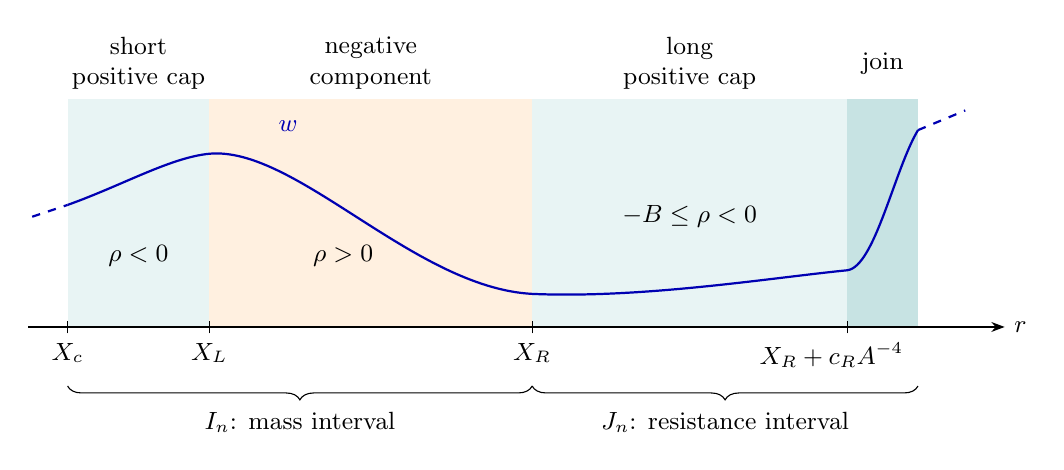
\begin{tikzpicture}[x=1cm,y=1cm,>=Stealth,font=\small]
\fill[teal!9] (.5,0) rectangle (2.3,2.9);
\fill[orange!12] (2.3,0) rectangle (6.4,2.9);
\fill[teal!9] (6.4,0) rectangle (10.4,2.9);
\fill[teal!22] (10.4,0) rectangle (11.3,2.9);
\draw[->] (0,0)--(12.4,0) node[right] {$r$};
\draw[thick,blue!70!black]
 (.5,1.55) .. controls (1.2,1.8) and (1.8,2.15) .. (2.3,2.2)
 .. controls (3.4,2.3) and (4.9,.5) .. (6.4,.42)
 .. controls (7.8,.36) and (9.4,.62) .. (10.4,.72)
 .. controls (10.75,.76) and (11.0,2.0) .. (11.3,2.5);
\draw[thick,blue!70!black,dashed] (11.3,2.5)--(11.9,2.75);
\draw[thick,blue!70!black,dashed] (.05,1.4)--(.5,1.55);
\foreach \x/\lab in {.5/X_c,2.3/X_L,6.4/X_R}{
 \draw (\x,-.08)--(\x,.08); \node[below] at (\x,-.08) {$\lab$};}
\draw (10.4,-.08)--(10.4,.08);
\node[below] at (10.2,-.08) {$X_R+c_RA^{-4}$};
\node[align=center] at (1.4,3.35) {short\\positive cap};
\node[align=center] at (4.35,3.35) {negative\\component};
\node[align=center] at (8.4,3.35) {long\\positive cap};
\node[align=center] at (10.85,3.35) {join};
\node at (1.4,.9) {$\rho<0$};
\node at (4.0,.9) {$\rho>0$};
\node at (8.4,1.4) {$-B\le\rho<0$};
\node[blue!70!black] at (3.3,2.55) {$w$};
\draw[decorate,decoration={brace,mirror,amplitude=5pt}]
 (.5,-.75)--(6.4,-.75) node[midway,below=6pt] {$I_n$: mass interval};
\draw[decorate,decoration={brace,mirror,amplitude=5pt}]
 (6.4,-.75)--(11.3,-.75) node[midway,below=6pt] {$J_n$: resistance interval};
\end{tikzpicture}
\caption{One cell and the join following it, in the direction of
increasing $r$ (not to scale). The tick marks give the values of the
model coordinate $X$. Each of the three parts of the cell has radial
length comparable to $A_n$; the join has length comparable to
$A_n^{12}$ or $A_{n\pm1}^{12}$. Along the join the profile rises by a
factor $e^{4n^2+o(n^2)}$. The intervals $I_n$ and $J_n$ are used in
Section~\ref{subsec:mass-resistance}.}
\label{fig:cell}
\end{figure}

\begin{lemma}[The cell is a radial profile]\label{lem:cell}
On the retained interval $r_X>0$. More precisely, with constants
independent of $n$,
\begin{equation}\label{eq:rad-eq-rm6a}
 r_X(X_c)=\tfrac38A+O(A^2),\qquad
 r(X_c)=1-\tfrac{15}{16}A+O(A^2),
\end{equation}
and
\begin{equation}\label{eq:rad-eq-rm6}
 \begin{gathered}
 r=1+O(A),\qquad cA^5\le r_X\le CA,\qquad
 r_X\asymp A^5\ \text{on the long positive cap},\\
 \Delta r\asymp A,\qquad
 \int_{X_c}^{X_R}r_X^2\,dX\asymp A^2,\qquad
 \int_{\text{each positive cap}}\sqrt{-\rho}\,dX\asymp\sqrt A .
 \end{gathered}
\end{equation}
Here $\Delta r$ is the radial length of each of the three parts.
\end{lemma}

\begin{proof}
On $[X_c,X_R]$ the integral $\int(Y-X_c)|\rho(Y)|\,dY$ is $O(A)$, so
the Volterra equation
\[
 r(X)=1-r_X(X_R)\,(X_R-X)
       -\int_X^{X_R}(Y-X)\,\rho(Y)\,r(Y)\,dY
\]
gives $r=1+O(A)$ there. For \eqref{eq:rad-eq-rm6a} evaluate the leading
terms with $t=e^{-Y}$:
\[
 \int_0^{3/2}(1-t)\,dt=\frac38,\qquad
 \int_0^{3/2}\log\frac{3/2}{t}\,(1-t)\,dt=\frac{15}{16};
\]
the constant $B$ contributes only $O(B\log^2(A/B))=o(A^2)$.

On the negative component $r_X(X)=r_X(X_R)+\int_X^{X_R}\rho\,r>0$. On
the short positive cap $r_{XX}=-\rho r>0$, so the minimum of $r_X$ is
its value at $X_c$, which is positive by \eqref{eq:rad-eq-rm6a}. On
the long positive cap $0<r_{XX}\le Br$; since
$B\cdot c_RA^{-4}\asymp c_RA^5$, comparison with $r_{XX}=Br$ shows
$r_X\asymp A^5$ there, and $r$ changes by $O(A)$. Taking $c_R$ small
keeps $r$ in a fixed positive range throughout. The remaining
statements follow by integration: $r_X\asymp A$ on a fixed part of
$[X_c,X_R]$ and $r_X\le CAe^{-X}+CA^5$ on all of it; on the long cap
$-\rho\asymp B$ away from $X_R$ and $\sqrt B\,A^{-4}\asymp\sqrt A$; on
the short cap $-\rho\asymp A$ on a fixed subinterval.
\end{proof}

The last quantity in \eqref{eq:rad-eq-rm6} measures the strength of a
positive cap as a buffer. On a cap the equation $L_ju=0$ reads
$u_{XX}=j^2|\rho|\,u$, whose solutions grow or decay like
$\exp(\pm j\int\sqrt{|\rho|}\,dX)$. We call
\begin{equation}\label{eq:cap-action}
 \tau_{n,j}=j\sqrt{A_n}
\end{equation}
the \emph{action} of the positive caps of cell $n$ at frequency $j$.
The caps of cell $n$ decouple their two sides when $\tau_{n,j}$ is
large, and are transparent when it is small.

\subsection{Joining the cells}
\label{subsec:joins}

\paragraph{Radii.}
Since \eqref{eq:rad-eq-rm4} is linear in $r$, we may multiply $r$ by a
\emph{radius factor} $\mathfrak r_n>0$ without changing $\rho$ or the
operators $H_{j,M}$. Between a cell and its neighbour in the direction
of increasing $r$ we insert a \emph{join}: an interval of length
\begin{equation}\label{eq:rad-eq-rm7}
 \ell_{n,m}=c_C\,r_o\,\min(A_n,A_m)^{12},\qquad m=n\pm1,
\end{equation}
where $n,m$ are the indices of the two cells, $r_o$ is the radius at
which the join starts, and $c_C>0$ is a fixed constant. The radius
factor of the neighbour is chosen so that it starts at $r_o+\ell_{n,m}$.
By Lemma~\ref{lem:cell} the ratio of consecutive radius factors is
$1+O(A_n+A_m)$, so the recursion converges at either end; on the left
the limiting radius may be prescribed. Hence all radii stay in a
compact subset of $(0,\infty)$, the $\mathfrak r_n$ are bounded above
and below, and the cells accumulate at finite endpoints.

\paragraph{The profile on a join.}
Let $W_L$ and $W_R$ be the values of $w$ at the two ends of a join.
At the right endpoint the join leads from the end of the long cap of
cell $n$, where $w\asymp\lambda_nA_n^5$, to the beginning of cell
$n+1$, where $w\asymp\lambda_{n+1}A_{n+1}$; at the left endpoint it
leads from cell $n+1$ to cell $n$. In both cases the profile rises,
and
\begin{equation}\label{eq:height-contrast-new}
 \log\frac{W_R}{W_L}=4n^2+O(n^{3/2}+n).
\end{equation}
To match the two neighbouring profiles to infinite order, let
$f_L,f_R$ be the logarithms of the two neighbouring model profiles,
choose cutoffs $\chi_L,\chi_R$ with disjoint supports, equal to one
near the left and right end of the join respectively, and define
$f=\log w$ on the join by
\begin{equation}\label{eq:rad-eq-rm8}
 f'=\chi_Lf_L'+\chi_Rf_R'+C_1\,(1-\chi_L-\chi_R),
 \qquad
 C_1=\frac{\log(W_R/W_L)-\int\chi_Lf_L'-\int\chi_Rf_R'}
             {\int(1-\chi_L-\chi_R)},
\end{equation}
with $f=\log W_L$ at the left end. Then $f=\log W_R$ at the right end,
and $w=e^f$ agrees with the two models to infinite order. The two
integrals in the numerator are $O(\ell_{n,m}/\min(A_n,A_m))$, while the
required change of height is of order $n^2$. Hence $C_1>0$, and after
$N$ is increased
\begin{equation}\label{eq:join-slope}
 \frac{w'}{w}\ge\frac2r\qquad\text{on every join.}
\end{equation}

\paragraph{Why the exponent $12$.}
The exponent in \eqref{eq:rad-eq-rm7} looks extravagant; it is chosen
so that a join is invisible to every frequency that has to cross it
carefully. The contrast of heights across the join costs a factor
$e^{4n^2+o(n^2)}$. The largest frequency assigned to cell $n$
(Section~\ref{subsec:bands}) satisfies $j^2\le e^{n^2+o(n^2)}$. The
length of the join contributes $e^{-12n^2+o(n^2)}$. The product is
$e^{-7n^2+o(n^2)}$, far below the matching angle $e^{-n^2}$ that we
shall allow. The same choice makes the mass and the resistance of a
join negligible in Section~\ref{subsec:mass-resistance}. No minimal
exponent is needed.

\begin{lemma}[Flatness and coefficient bounds]\label{lem:tail-flat}
Let $d_\partial$ be the distance to the endpoint. On cell $n$ and on
the joins adjacent to it,
\begin{equation}\label{eq:geometry-endpoint-distance}
 cA_{n+1}\le d_\partial\le CA_n,
 \qquad \log\frac{d_0}{d_\partial}=n^2+O(n)
\end{equation}
for a fixed $d_0>0$, and for every $s\ge0$
\begin{equation}\label{eq:geometry-profile-jets}
 \begin{gathered}
 e^{-n^{5/2}-Cn^2}\le w\le e^{-n^{5/2}+Cn^2},\\
 |\partial_r^sw|\le C_s\,e^{-n^{5/2}+C_sn^2},\qquad
 |\partial_r^s(w^{-1})|\le C_s\,e^{n^{5/2}+C_sn^2}.
 \end{gathered}
\end{equation}
The constants do not depend on the height ratios $\sigma_k\in[1,2]$.
Consequently $w$ extends smoothly by zero across the endpoint, and
all fixed-order derivatives of $w$ and of $w^{-1}$ on cell $n$ are
bounded by coefficient powers $C_s\mathcal E_n^{C_s}$.
\end{lemma}

\begin{proof}
The length of cell $n$ is comparable to $A_n$ by
Lemma~\ref{lem:cell}, and $A_{n+1}/A_n=e^{-2n-1}(1+o(1))$; summing the
lengths of the cells beyond $n$ gives
\eqref{eq:geometry-endpoint-distance}. All lengths of intervals and
their reciprocals are bounded by $e^{Cn^2}$. On a model
$\partial_r=r_X^{-1}\partial_X$ and $r_X\ge c\,\mathfrak r_nA_n^5$, and
the differential equation \eqref{eq:rad-eq-rm4} bounds every fixed
derivative of $\log r_X$ by $e^{C_sn^2}$. On a join
\eqref{eq:rad-eq-rm8} gives the same bound for $\log w$. A derivative
of $e^{\pm\log w}$ is $e^{\pm\log w}$ times a polynomial in the
derivatives of $\log w$, which proves
\eqref{eq:geometry-profile-jets}. Since
$e^{-n^{5/2}+C_sn^2}d_\partial^{-k}\to0$ for all $s,k$ by
\eqref{eq:geometry-endpoint-distance}, the extension by zero is
smooth. The last statement follows from $n^2=o(q_n)$.
\end{proof}

\subsection{Why a mass--resistance chain appears}
\label{subsec:mass-resistance}

We now study $L_ju=0$ on a tail. The equation has the unpleasant
feature that its zeroth-order coefficient $j^2w'/r$ is enormous on the
joins. A change of the unknown removes it.

\begin{lemma}[Gauge]\label{lem:gauge}
Let $y=\log r$ and $u=r^{j^2}V$. Then
\begin{equation}\label{eq:rad-eq-rm13}
 r^2L_ju=r^{j^2}\,\frac{w}{\mathsf p_j}\,
 \bigl[(\mathsf p_jV_y)_y+\Lambda\,\mathsf p_jV\bigr],
 \qquad \mathsf p_j=w\,r^{2j^2-1},\qquad \Lambda=j^2(j^2-1).
\end{equation}
\end{lemma}

\begin{proof}
In the variable $y$ one has
$r^2L_ju=wu_{yy}+(w_y-w)u_y-j^2w_yu$. Substituting
$u=e^{j^2y}V$, the terms containing $w_yV$ cancel, and what remains is
$e^{j^2y}\,[wV_{yy}+((2j^2-1)w+w_y)V_y+(j^4-j^2)wV]$.
\end{proof}

So $L_ju=0$ is equivalent to the Sturm--Liouville equation
$-(\mathsf p_jV_y)_y=\Lambda\,\mathsf p_jV$, in which the profile
enters only through the density $\mathsf p_j$. For $j=2$ this density
is $\mathsf p=wr^7$ and $\Lambda=12$.

\paragraph{Mass and resistance.}
Divide each cell into two intervals (Figure~\ref{fig:cell}): the
\emph{mass interval} $I_n$, consisting of the short positive cap and
the negative component, and the \emph{resistance interval} $J_n$,
consisting of the long positive cap and the join that follows it in
the direction of increasing $r$. For a density $\mathsf p$ define
\begin{equation}\label{eq:mass-resistance-def-new}
 \mu_n=\int_{I_n}\mathsf p\,dy,\quad
 R_n^I=\int_{I_n}\frac{dy}{\mathsf p},\quad
 \nu_n=\int_{J_n}\mathsf p\,dy,\quad
 R_n=\int_{J_n}\frac{dy}{\mathsf p}.
\end{equation}
We call $\mu_n,\nu_n$ \emph{masses} and $R_n^I,R_n$
\emph{resistances}. The names come from the following elementary
observation about an equation $-(\mathsf pV_y)_y=\Lambda\mathsf pV$.
\begin{itemize}
\item On an interval of small resistance the value $V$ is nearly
 constant, and the flux $\mathsf pV_y$ changes by $-\Lambda$ times the
 mass times that value.
\item On an interval of small mass the flux is nearly constant, and
 the value changes by the flux times the resistance.
\end{itemize}
In our tails $I_n$ carries almost all the mass and almost no
resistance, and $J_n$ the opposite. Let $a_n$ be the value of $V$ on
$I_n$ and $\varphi_n$ the flux on $J_n$. The two rules give
\[
 \varphi_n=\varphi_{n-1}-\Lambda\mu_na_n,\qquad
 a_{n+1}=a_n+R_n\varphi_n .
\]
Eliminating the fluxes yields a three-term recurrence for the $a_n$
whose diagonal coefficient $\Lambda\mu_n$ is very large compared with
the off-diagonal coefficients $1/R_n$. For a solution that decays, the
dominant balance is $a_{n+1}\approx-a_n/(\Lambda\mu_{n+1}R_n)$: the
values alternate in sign and decrease rapidly
(Figure~\ref{fig:mass-resistance-chain}).
Section~\ref{subsec:exact-reduction} turns this picture into an exact
statement.

\begin{figure}[htbp]
\centering
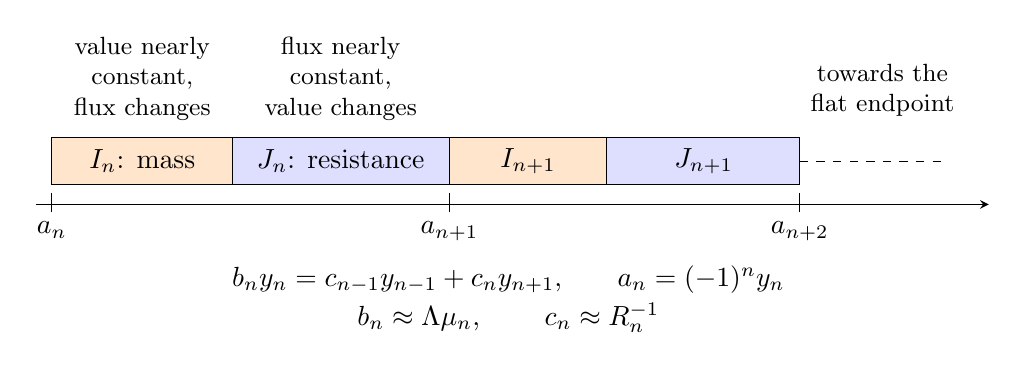
\begin{tikzpicture}[x=1cm,y=1cm,>=stealth]
\draw[->] (0,0)--(12.1,0);
\node[align=center,font=\small] at (10.75,1.45)
 {towards the\\flat endpoint};
\draw[fill=orange!20] (.2,.25) rectangle (2.5,.85);
\draw[fill=blue!13] (2.5,.25) rectangle (5.25,.85);
\draw[fill=orange!20] (5.25,.25) rectangle (7.25,.85);
\draw[fill=blue!13] (7.25,.25) rectangle (9.7,.85);
\draw[dashed] (9.7,.55)--(11.5,.55);
\node at (1.35,.55) {$I_n$: mass};
\node at (3.87,.55) {$J_n$: resistance};
\node at (6.25,.55) {$I_{n+1}$};
\node at (8.48,.55) {$J_{n+1}$};
\foreach \x/\lab in {.2/a_n,5.25/a_{n+1},9.7/a_{n+2}}
 {\draw (\x,-.1)--(\x,.15);\node[below] at (\x,-.1) {$\lab$};}
\node[align=center,font=\small] at (1.35,1.6) {value nearly\\constant,\\flux changes};
\node[align=center,font=\small] at (3.87,1.6) {flux nearly\\constant,\\value changes};
\node[align=center] at (6,-1.2)
 {$b_n y_n=c_{n-1}y_{n-1}+c_ny_{n+1}$,\qquad $a_n=(-1)^ny_n$\\[2pt]
 $b_n\approx\Lambda\mu_n$, \qquad $c_n\approx R_n^{-1}$};
\end{tikzpicture}
\caption{The intervals of a tail and the node equation satisfied by
the values $a_n$ of a solution at the entrances of the mass intervals.
Large products $\Lambda\mu_nR_n$ make successive node values of the
decaying solution small.}
\label{fig:mass-resistance-chain}
\end{figure}

\begin{lemma}[Masses and resistances of the tail]\label{lem:mass-res}
For the density $\mathsf p=wr^7$ on the tail constructed above,
\begin{equation}\label{eq:rad-eq-rm10}
 \mu_n\asymp\lambda_nA_n^2,\qquad
 R_n^I\le\frac{C}{\lambda_n}\log\frac{A_n}{B_n},\qquad
 \nu_n\le C\lambda_nA_n^6,\qquad
 R_n\asymp\frac1{\lambda_nA_n^{4}},
\end{equation}
hence
\begin{equation}\label{eq:rad-eq-rm11}
 \mu_nR_n\asymp A_n^{-2},\qquad
 \mu_nR_n^I\le CA_n^2\log\frac{A_n}{B_n},\qquad
 \nu_nR_n\le CA_n^2,
\end{equation}
and
\begin{equation}\label{eq:rad-eq-rm12}
 \log(\mu_{n+1}R_n)=2n^2+O(n^{3/2}+n).
\end{equation}
\end{lemma}

\begin{proof}
Since $dy=dr/r$ and $dr=r_X\,dX$, the measures in
\eqref{eq:mass-resistance-def-new} are $wr^6\,dr$ and $dr/(wr^8)$,
and on a model $w\,dr=\lambda r_X^2\,dX$ and $dr/w=dX/\lambda$. The
radius is bounded above and below, so \eqref{eq:rad-eq-rm6} gives
\eqref{eq:rad-eq-rm10} for the model parts. A join of length $\ell$
adds at most $W_R\ell$ to the mass and $\ell/W_L$ to the resistance of
$J_n$; relative to $\nu_n$ and $R_n$ these are
$e^{-7n^2+O(n^{3/2}+n)}$ and $e^{-11n^2+O(n)}$. The products
\eqref{eq:rad-eq-rm11} follow, and so does \eqref{eq:rad-eq-rm12}
from $\log(\lambda_{n+1}/\lambda_n)=O(n^{3/2})$ and
$\log(A_{n+1}^2/A_n^4)=2n^2+O(n)$.
\end{proof}

\paragraph{Other frequencies.}
For a general frequency the density is $\mathsf p_j$. After division
by the constant $r_\partial^{2(j^2-4)}$, where $r_\partial$ is the
radius of the endpoint,
\[
 \frac{\mathsf p_j}{\mathsf p}
 =\Bigl(\frac r{r_\partial}\Bigr)^{2(j^2-4)},
\]
and on the part of the tail beyond cell $N'$ the logarithm of this
ratio is bounded by $Cj^2A_{N'}$. So
Lemma~\ref{lem:mass-res} holds for $\mathsf p_j$, with uniform
constants, on every part of the tail where $j^2A_{N'}$ is bounded. We
shall use the slightly stronger condition
\begin{equation}\label{eq:deep-frequency-condition-new}
 j^2A_{N'}\sqrt{\log(A_{N'}/B_{N'})}\le c
\end{equation}
for a small constant $c$; by \eqref{eq:rad-eq-rm11} it makes
$\Lambda\mu_nR_n^I$ and $\Lambda\nu_nR_n$ small for all $n\ge N'$.

\subsection{The exact reduction to a recurrence}
\label{subsec:exact-reduction}

Use the coordinate $x=\log r$ at the right endpoint and $x=-\log r$ at
the left endpoint, so that $x$ always increases outward. At the left
endpoint the outward order of the intervals is
$J_N,I_N,J_{N+1},I_{N+1},\ldots$. Within this subsection only, the
resistance interval that follows $I_n$ in the outward direction is
therefore renamed $J_n$ also at the left endpoint (it is the original
$J_{n+1}$), and the first interval $J_N$ is treated as a separate
\emph{initial resistance edge} $J_0$ with resistance $R_0$ and mass
$\nu_0$. The shift of index affects only the lower-order terms of
\eqref{eq:rad-eq-rm12}.

The following definition isolates what the reduction needs.

\begin{definition}[Deep tail]\label{def:deep-tail}
Let $\mathsf p>0$ be a density on a half-line in $x$ which is divided
into consecutive intervals $I_n,J_n$ ($n\ge N'$), possibly preceded by
an initial resistance edge $J_0$, and let $\Lambda>0$. With the masses
and resistances \eqref{eq:mass-resistance-def-new} formed with $dx$,
the data form a \emph{deep tail} with constants $\eta\ll1\ll K$ if for
all $n$
\begin{equation}\label{eq:rad-eq-dg1}
 \begin{gathered}
 \Lambda\mu_nR_n^I+\Lambda\nu_nR_n\le\eta,\qquad
 \Lambda\mu_nR_n\ge K,\quad \Lambda\mu_{n+1}R_n\ge K,\\
 \nu_n\le\eta\,\min(\mu_n,\mu_{n+1}),
 \end{gathered}
\end{equation}
and if, when there is an initial edge,
$\Lambda\mu_{N'}R_0\ge K$, $\Lambda\nu_0R_0\le\eta$ and
$\nu_0\le\eta\mu_{N'}$.
\end{definition}

By Lemma~\ref{lem:mass-res} and the remark on other frequencies, the
part of a constructed tail beyond cell $N'$ is a deep tail for
$\mathsf p_j$ and $\Lambda=j^2(j^2-1)$ whenever
\eqref{eq:deep-frequency-condition-new} holds and $N'$ is large
enough; $\eta$ and $K^{-1}$ can be made as small as we wish.

\begin{lemma}[Deep inverse and the natural line]
\label{lem:radial-deep-inverse}
\label{lem:radial-flat-line}
On a deep tail, with $\eta$ and $K^{-1}$ sufficiently small, let
\[
 A_{\mathsf p}=-\mathsf p^{-1}\partial_x\,\mathsf p\,\partial_x
\]
act in $L^2(\mathsf p\,dx)$ with the Dirichlet condition at the
entrance and the Friedrichs condition at the outer endpoint.
\begin{enumerate}
\item $\|(A_{\mathsf p}-\Lambda)^{-1}\|\le C/\Lambda$.
\item Up to multiples, the equation $(A_{\mathsf p}-\Lambda)V=0$ has
 exactly one solution which is square integrable for
 $\mathsf p\,dx$ near the outer endpoint. Its values $a_n$ at the
 entrances of the mass intervals $I_n$ are nonzero and alternate in
 sign: $a_n=(-1)^ny_n$ with $y_n>0$ and
 \begin{equation}\label{eq:rad-eq-dg4}
  \frac{y_{n+1}}{y_n}
  =\frac{1+O(\eta)+O(K^{-1})}{\Lambda\mu_{n+1}R_n},
  \qquad
  \frac{\sqrt{\mu_{n+1}}\,y_{n+1}}{\sqrt{\mu_n}\,y_n}\le\frac CK<\frac12 .
 \end{equation}
\item For the constructed tails and $\mathsf p=\mathsf p_j$, the
 corresponding solution $u=r^{j^2}V$ of $L_ju=0$ is smooth and flat at
 the endpoint.
\end{enumerate}
\end{lemma}

The line spanned by the solution in (ii) is the \emph{natural line} of
Section~\ref{subsec:layout}.

\begin{proof}
The reduction is carried out on the differential equation itself, so
that the operator norm and the endpoint condition come out of one
argument. An \emph{edge} is $\mathsf E_n=I_n\cup J_n$; its two
endpoints are \emph{nodes}, and node $n$ is the entrance of $I_n$.

\step{1: one edge in the resistance coordinate}
On $\mathsf E_n$ introduce $ds=dx/\mathsf p$. The edge has length
$L_n=R_n^I+R_n$ in $s$; with $\omega=\mathsf p^2$ we have
$\mathsf p\,dx=\omega\,ds$ and
\[
 (A_{\mathsf p}-\Lambda)u=f
 \quad\Longleftrightarrow\quad -u_{ss}-\Lambda\,\omega\,u=\omega f .
\]
The Dirichlet Green function of $-\partial_s^2$ on the edge is
$G_0(s,t)=\min(s,t)\,[L_n-\max(s,t)]/L_n$. The small quantities are
\[
 \delta_n^{\rm edge}=\Lambda\int\omega(s)\,G_0(s,s)\,ds\le3\eta,
 \qquad \frac{R_n^I}{L_n}\le\frac\eta K ,
\]
by the first line of \eqref{eq:rad-eq-dg1}. The inequality
$G_0(s,z)G_0(z,t)\le G_0(s,t)G_0(z,z)$ bounds the Neumann series of
the Dirichlet Green function $G_\Lambda$ of $-\partial_s^2-\Lambda\omega$
term by term. With $l_0=1-s/L_n$, $l_1=s/L_n$, and $v_0,v_1$ the
solutions of the homogeneous equation on the edge with boundary values
$(1,0)$ and $(0,1)$, the same argument applies with one factor
replaced by $l_i$, and we obtain
\begin{equation}\label{eq:rad-eq-dg2}
 G_0\le G_\Lambda\le(1-\delta_n^{\rm edge})^{-1}G_0,
 \qquad l_i\le v_i\le(1-\delta_n^{\rm edge})^{-1}\,l_i .
\end{equation}
For $u$ vanishing at both ends of the edge,
$\Lambda\int\omega|u|^2\le\delta_n^{\rm edge}\int|u_s|^2$. Hence the
direct sum $G_D$ of the Dirichlet inverses of all edges has norm at
most $C\eta/\Lambda$ on $L^2(\mathsf p\,dx)$.

\step{2: the boundary matrix of an edge}
For boundary values $(a,a')$ at the two ends of $\mathsf E_n$ the
homogeneous solution is $av_0+a'v_1$, and its outward derivatives at
the two ends, in the variable $s$, are given by the matrix
\[
 \begin{pmatrix}d_{n,0}&-c_n\\-c_n&d_{n,1}\end{pmatrix},\qquad
 c_n=\frac1{L_n}+\Lambda\int\omega\,l_0v_1,\qquad
 d_{n,i}=\frac1{L_n}-\Lambda\int\omega\,l_iv_i ;
\]
the formulas follow from Green's identity with the functions $l_i$.
Since $l_0l_1=G_0(s,s)/L_n$, \eqref{eq:rad-eq-dg2} gives
\begin{equation}\label{eq:rad-eq-dg3}
 c_n=\frac{1+O(\eta)}{R_n},\qquad
 b_n:=-d_{n-1,1}-d_{n,0}
       =\Lambda\mu_n\,\bigl(1+O(\eta)+O(K^{-1})\bigr).
\end{equation}
For the second formula: on $I_n$ we have $l_0=1+O(R_n^I/L_n)$, so
that interval contributes $\Lambda\mu_n(1+O(\eta))$ to
$\Lambda\int\omega\,l_0v_0$, and $J_n$ contributes at most
$C\Lambda\nu_n\le C\eta\Lambda\mu_n$. The preceding edge contributes
to $\Lambda\int\omega\,l_1v_1$ at most $C\Lambda$ times
$\nu_{n-1}+\mu_{n-1}(R_{n-1}^I/L_{n-1})^2$, and the second term is at
most $\eta^2K^{-2}\mu_n$ by \eqref{eq:rad-eq-dg1}. The two terms
$1/L_n$ and $1/L_{n-1}$ are at most $\Lambda\mu_n/K$ each. The same
computation covers an initial resistance edge.

\step{3: interpolation of node values}
For a sequence $a=(a_n)$ of node values let $Ta$ be the function which
on each edge is the homogeneous solution with these boundary values,
$(Ta)|_{\mathsf E_n}=a_nv_0+a_{n+1}v_1$. Let
$\mathfrak h=\ell^2(\mu_n)$. Then
\begin{equation}\label{eq:rad-eq-dj1}
 c\,\|a\|_{\mathfrak h}^2\le\|Ta\|_{L^2(\mathsf p\,dx)}^2
                         \le C\,\|a\|_{\mathfrak h}^2 .
\end{equation}
Indeed, by \eqref{eq:rad-eq-dg2} the function $Ta$ is close to $a_n$
on $I_n$, which carries the mass $\mu_n$. On $I_n$ the neighbouring
value enters with the factor $l_1\le R_n^I/L_n$, and the sum of these
contributions is $O(\eta^2/K^2)\,\|a\|_{\mathfrak h}^2$ after a shift
of index. The contribution of $J_n$ is controlled by the last
inequality of \eqref{eq:rad-eq-dg1}.

\step{4: the node operator}
The quadratic form of $A_{\mathsf p}-\Lambda$ on interpolants is, by
Step~2,
\[
 (\mathcal Da,a)_{\mathfrak h}
   =-\sum_n b_n|a_n|^2-2\operatorname{Re}\sum_n c_n\,a_n\overline{a_{n+1}} ,
\]
which defines a symmetric operator $\mathcal D$ on $\mathfrak h$. In
the coordinates $\sqrt{\mu_n}\,a_n$ its diagonal entries have size
$\Lambda$ by \eqref{eq:rad-eq-dg3}, while each off-diagonal entry is
bounded by $C/(R_n\sqrt{\mu_n\mu_{n+1}})\le C\Lambda/K$. By diagonal
dominance
\[
 \|\mathcal D^{-1}\|\le\frac C\Lambda ,
\]
independently of the number of edges.

\step{5: the inverse}
These algebraic facts give an inverse of the operator because they
respect its form domain. On the one hand, the energy of an interpolant
is bounded by $C\Lambda\|a\|_{\mathfrak h}^2$, by the formula for
$\mathcal D$ and \eqref{eq:rad-eq-dj1}. On the other hand, averaging
$u(x_n)-u(x)$ over $I_n$, where $x_n$ is node $n$, gives
\[
 \mu_n\,|u(x_n)|^2\le2\,\|u\|_{L^2(I_n,\mathsf p\,dx)}^2
            +2\mu_nR_n^I\int_{I_n}|u_s|^2\,ds ,
\]
so every function in the form domain has node values in $\mathfrak h$
and splits as $u=Ta+u^\circ$ with $u^\circ$ vanishing at all nodes.
The two parts are orthogonal for the form of $A_{\mathsf p}-\Lambda$,
because $Ta$ solves the homogeneous equation on each edge. Therefore
\begin{equation}\label{eq:rad-eq-dj2}
 (A_{\mathsf p}-\Lambda)^{-1}=G_D+T\,\mathcal D^{-1}T^*,
 \qquad (T^*f)_n=\frac1{\mu_n}\int\mathsf p\,(T\mathbf e_n)\,f\,dx ,
\end{equation}
where $\mathbf e_n$ is the $n$th unit sequence. Truncations of the
tail by a Dirichlet wall at a far node obey the same formula and
converge strongly, since the diagonally dominant series for
$\mathcal D^{-1}$ converges uniformly on finite compressions; their
limit is the Friedrichs realization identified by the decomposition
of the form domain. Steps~1, 3 and~4 now give~(i).

\step{6: the decaying solution}
A homogeneous solution is the interpolant of its node values, and
continuity of the flux at node $n$ reads
$-b_na_n=c_{n-1}a_{n-1}+c_na_{n+1}$. With $a_n=(-1)^ny_n$ this is
\[
 b_n\,y_n=c_{n-1}\,y_{n-1}+c_n\,y_{n+1}.
\]
Put $\epsilon_n=c_n^2/(b_nb_{n+1})\le C/K^2$ and
$t_n=b_{n+1}y_{n+1}/(c_ny_n)$. Eliminating backwards from the outer
end,
\[
 t_n=\frac1{1-\epsilon_{n+1}t_{n+1}} .
\]
For large $K$ these maps preserve the interval $[1,2]$ and contract
it by a factor at most $\tfrac12$. Hence the solutions with a
Dirichlet wall at a far node converge, as the wall recedes, to a
unique sequence with $t_n\in[1,2]$ for all $n$. By
\eqref{eq:rad-eq-dg3} it satisfies \eqref{eq:rad-eq-dg4}, and by
\eqref{eq:rad-eq-dj1} its interpolant is square integrable.

Any solution independent of this one has node values of the form
\[
 z_n=y_n\Bigl(C+\mathcal W\sum_{k<n}\frac1{c_ky_ky_{k+1}}\Bigr),
 \qquad\mathcal W\ne0 .
\]
Consecutive terms of the sum grow by a factor at least $cK^2$, so
eventually $|z_{n+1}/z_n|\asymp\Lambda\mu_nR_n$ and
$\sqrt{\mu_{n+1}}\,|z_{n+1}|\ge cK\sqrt{\mu_n}\,|z_n|$. On $I_n$ the
contribution of the neighbouring node is at most $C\eta$ times that of
node $n$ itself, so the $L^2(\mathsf p\,dx)$ norm of this solution
diverges. This proves the uniqueness in~(ii); in the language of
Sturm--Liouville theory, the outer endpoint is of limit-point type.

\step{7: flatness for the constructed tails}
Summing \eqref{eq:rad-eq-rm12} in \eqref{eq:rad-eq-dg4} gives, for
$k\ge m$,
\begin{equation}\label{eq:rad-eq-rm17}
 \left|\frac{a_k}{a_m}\right|
 \le\mathcal E_k^C\,\mathcal E_m^C\,e^{-(S_k-S_m)},
 \qquad\text{since}\quad
 2\sum_{n=m}^{k-1}n^2
 =\tfrac23(k^3-m^3)-(k^2-m^2)+\tfrac13(k-m),
\end{equation}
where the accumulated errors $O(n^{3/2}+n)$ and the quadratic terms
are absorbed by $q_k+q_m$. By Lemma~\ref{lem:tail-flat} every radial
derivative of fixed order costs at most $e^{C_sn^2}$ on cell $n$, and
the normalized gauge factor $(r/r_\partial)^{j^2}$ is bounded with
bounded inverse in the range \eqref{eq:deep-frequency-condition-new}.
Thus, after a normalization at the entrance, the solution and all its
derivatives of fixed order are bounded on cell $n$ by
$\mathcal E_n^{C_s}e^{-S_n}$, which tends to zero faster than every
power of $d_\partial$. This is~(iii).
\end{proof}

\begin{remark}\label{rem:line-continuity}
The contraction in Step~6 is uniform in the height ratios, so the
natural line depends continuously on $(\sigma_k)_{k\ge N}$ in the
product topology. This is used in
Lemma~\ref{lem:radial-product-selection}.
\end{remark}

\subsection{Localized bounds for the deep inverse}
\label{subsec:deep-green}

Later we need more than the operator norm: the kernel of the deep
inverse decays between distant cells.

\paragraph{The node Green matrix.}
Let $\mathsf N$ be the symmetric tridiagonal matrix with diagonal
entries $b_n$ and off-diagonal entries $-c_n$. Up to the signs
$(-1)^n$ and the weights $\mu_n$ it represents $-\mathcal D$, and by
Step~4 it is positive with a bounded inverse in the coordinates
$\sqrt{\mu_n}\,a_n$. Let $\Gamma=\mathsf N^{-1}$. Its diagonal
satisfies $b_m^{-1}\le\Gamma_{mm}\le Cb_m^{-1}$, by the Neumann series
with positive terms. For fixed $m$ the sequence $n\mapsto\Gamma_{nm}$,
$n\ge m$, is a decaying solution of the recurrence, so by uniqueness
\begin{equation}\label{eq:rad-eq-dj4}
 \Gamma_{nm}=\Gamma_{mm}\,\frac{y_n}{y_m}
 \le\frac{C}{\Lambda\mu_m}
      \prod_{k=m}^{n-1}\frac{1+C(\eta+K^{-1})}{\Lambda\mu_{k+1}R_k}
 \qquad(n\ge m),
\end{equation}
and symmetry gives the bound for $n<m$. The kernel of
$T\mathcal D^{-1}T^*$ in \eqref{eq:rad-eq-dj2} is built from $\Gamma$
with additional signs, which do not matter for absolute bounds, and
with at most two interpolation functions at each of its two
arguments; the kernel of $G_D$ lives on single edges. With
\eqref{eq:rad-eq-rm17} we conclude: for the constructed tails, the
part of the kernel of $(A_{\mathsf p}-\Lambda)^{-1}$ leading from cell
$m$ to cell $n$ has operator norm at most
\begin{equation}\label{eq:rad-eq-dj5}
 C\,\mathcal E_n^C\,\mathcal E_m^C\,e^{-|S_n-S_m|}.
\end{equation}

\paragraph{Return to radial units.}
Let $g=(r/r_\partial)^{j^2}$ and $\mathsf p^\circ=g^2w/r$, a constant
multiple of $\mathsf p_j$. By Lemma~\ref{lem:gauge},
\[
 L_j(gV)=-\frac{gw}{r^2}\,(A_{\mathsf p^\circ}-\Lambda)V,
 \qquad \mathsf p^\circ\,dx=\frac{g^2w}{r^2}\,dr,
 \qquad G_{L_j}(r,r')=-g(r)\,g(r')\,G_A(x,x'),
\]
where $G_{L_j}$ and $G_A$ are the kernels of the inverses of $L_j$,
with respect to $dr$, and of $A_{\mathsf p^\circ}-\Lambda$, with
respect to $\mathsf p^\circ dx$. The gauge factors are bounded above
and below, so \eqref{eq:rad-eq-dj5} holds for the inverse of $L_j$ in
the $dr$ pairing. In terms of the operator $B_j=-\varpi^{-1}L_j$ of
\eqref{eq:rad-eq-ha2},
\begin{equation}\label{eq:rad-eq-rm20}
 B_j=\frac1{12}\,g\,\bigl(A_{\mathsf p_j}-j^2(j^2-1)\bigr)\,g^{-1},
 \qquad \|B_{j,D}^{-1}\|\le\frac{C}{j^{4}}
\end{equation}
on a deep tail, where $B_{j,D}$ has the Dirichlet condition at the
entrance.

\paragraph{The entrance impedance.}
For the natural solution, the boundary matrix of Step~2 gives at a
mass entrance
$\mathsf pV_x/(\Lambda\mu_nV)=1+O(\eta)+O(K^{-1})$; if an initial
resistance edge comes first, the ratio of flux to value is instead
$-(1+O(\eta)+O(K^{-1}))/R_0$. In both cases the boundary term of
Green's identity at the outer endpoint vanishes for the natural
solution: at node $n$ it is bounded by $C\Lambda\mu_n|a_n|^2\to0$,
and finiteness of mass and energy identifies this with the limit at
the endpoint.

\subsection{Frequency bands: one transition cell at every frequency}
\label{subsec:bands}

How a cell acts on a solution depends on the frequency. If the action
$\tau_{n,j}=j\sqrt{A_n}$ of its caps is large, the cell is isolated
from its neighbours and is governed by its own spectral gap
(Lemma~\ref{lem:morse-arithmetic}). If the condition
\eqref{eq:deep-frequency-condition-new} holds, the cell is part of a
deep tail and is governed by the recurrence. The following
definition arranges that, at each frequency, at most one cell at each
end falls between the two regimes. Fix a large constant $C_*$ and put
\begin{equation}\label{eq:rad-eq-rm21}
 \jn_n=C_*\,q_n\,A_n^{-1/2},\qquad
 \mathcal I_n=\{j\ \text{even}:\ \jn_{n-1}\le j<\jn_n\}\quad(n>N),
\end{equation}
and let the first band $\mathcal I_N$ consist of all even $j$ with
$2\le j<\jn_N$. The \emph{bands} $\mathcal I_n$, $n\ge N$, partition
the even frequencies. For $j\in\mathcal I_n$:
\begin{itemize}
\item every earlier cell $m<n$ has large action,
 $\tau_{m,j}=j\sqrt{A_m}\ge C_*q_m$. These cells, together with the
 central model, form the \emph{inner region};
\item cell $n$ is the \emph{transition cell};
\item the cells $m>n$ form a deep tail, because
 \begin{equation}\label{eq:rad-eq-rm22}
  j^2A_{n+1}\sqrt{\log(A_{n+1}/B_{n+1})}
  \le C\,C_*^2\,q_n^2\,\frac{A_{n+1}}{A_n}\,(n+1)\longrightarrow0 .
 \end{equation}
\end{itemize}
So there is no range of frequencies left unexamined between the local
spectral inverses and the deep inverse. The decomposition depends on
the frequency; the profile does not. This structure is the key to the
assembly of the global inverse in
Section~\ref{sec:radial-reference-inverse}.

\paragraph{An auxiliary cone at the entrance of a tail.}
To define an incoming line for the first band, attach at the entrance
of each tail an auxiliary cone $w=cr$. For the right tail the cone is
continued inward to $r=0$, for the left tail outward to $r=\infty$.
The transition between cone and first cell is a short positive
interval with $rw'/w\ge1$, constructed by applying
\eqref{eq:rad-eq-rm8} to $\log(w/r)$. On the cone, in $y=\log r$,
\[
 B_j=\tfrac1{12}\,(-\partial_y^2+j^2),\qquad
 \varpi\,dr=12c\,dy ;
\]
the solutions regular at the far end of the cone are $r^{j}$ for the
right tail and $r^{-j}$ for the left tail, and the Dirichlet inverse
of $B_j$ has norm at most $12/j^2$. The cone serves only to specify
an incoming line. The final profile retains a finite piece of it, the
\emph{cone head}.

\subsection{Choosing the heights so that the lines do not meet}
\label{subsec:height-selection}

Fix an endpoint, a band index $n$ and a frequency
$j\in\mathcal I_n$. Consider the join which precedes cell $n$ in the
outward order (for $n=N$: the transition from the auxiliary cone).
Let $W_{\rm in}$ be the value of the profile at its inner end and
$\sigma_nW^0_{\rm out}$ its value at the outer end. By
\eqref{eq:rad-eq-js2}, $W_{\rm in}$ does not depend on $\sigma_n$,
and $W^0_{\rm out}$ is the outer value for $\sigma_n=1$. Put
\begin{equation}\label{eq:rad-eq-js4}
 \Xi_n=\frac{W^0_{\rm out}}{W_{\rm in}},\qquad
 \Upsilon_n=\max(\Xi_n,\Xi_n^{-1}),\qquad
 \log\Upsilon_n=4n^2+O(n^{3/2}+n).
\end{equation}
At the first join the amplitude $c$ of the auxiliary cone is chosen,
independently of $\sigma_N$, so that the contrast is the same. The
radii and all cut points are independent of the height ratios.

The role of $\sigma_n$ is the following. Everything beyond the join is
multiplied by $\sigma_n$; this does not change the homogeneous
equation there, hence not the natural line. The incoming line is
determined by what lies before the join, and does not depend on
$\sigma_n$ either. What $\sigma_n$ changes is the scale of the flux
$wu'$ by which the two lines are compared across the join. We show
that this is enough to move them apart.

\paragraph{A state variable adapted to the join.}
On a join $w'/w$ is huge, and the pair $(u,wu')$ is not a convenient
state. Define instead
\begin{equation}\label{eq:rad-eq-js5}
 \zeta_j=\frac{ru_r}{j^2}-u .
\end{equation}
If $L_ju=0$, then $(w\zeta_j)'=-(j^2-1)\,wu_r/j^2$, in which $w'$ no
longer appears. For the state
$Y=(u,\ w\zeta_j/W_{\rm in})$ this gives
\begin{equation}\label{eq:rad-eq-js7}
 Y_r=\frac1r
 \begin{pmatrix}
 j^2&j^2\,W_{\rm in}/w\\
 -(j^2-1)\,w/W_{\rm in}&-(j^2-1)
 \end{pmatrix}Y .
\end{equation}
The coefficients involve only the sizes of $w$ and $w^{-1}$ on the
join, which lie between those at its ends. By the Volterra series,
the transfer matrix of \eqref{eq:rad-eq-js7} across the join differs
from the identity by at most $e^{\eta_{n,j}}-1$, where
\begin{equation}\label{eq:rad-eq-js14}
 \eta_{n,j}=Cj^2\,\frac{\ell_n}{r_{\min}}\,\Upsilon_n
 \le C\,C_*^2\,q_n^2\,e^{-7n^2+O(n^{3/2}+n)}=o(e^{-n^2}),
\end{equation}
$\ell_n$ being the length of the join. This is the computation behind
the exponent $12$ in \eqref{eq:rad-eq-rm7}: the steepness of the
profile on the join causes no difficulty.

\paragraph{The incoming line has a definite slope.}
As a stand-in for the incoming line we use the solution which vanishes
at a cut inside the positive cap preceding the join. The true incoming
line differs from it by an exponentially small amount, which is
accounted for in Section~\ref{subsec:terminal-matching}. Normalize
this solution to $u=1$ at the join. Then
\begin{equation}\label{eq:rad-eq-js6}
 a:=\frac{\zeta_j}{u}\in\bigl[-\tfrac32,-\tfrac12\bigr].
\end{equation}
Indeed, on the cap $u_{XX}=j^2|\rho|\,u$, and comparison with the
Riccati equation for a constant potential gives
$|u_X/u|\le Cj\sqrt b\,\coth(cj\sqrt A)$, where $b$ is the size of
$|\rho|$ on the cap and $A=A_{n-1}$. The cap is either the short one,
with $|\rho|\asymp A$, length $\asymp1$ in $X$ and $r_X\asymp A$, or
the long one, with $|\rho|\asymp A^9$, length $\asymp A^{-4}$ and
$r_X\asymp A^5$. In both cases $r_X\asymp\sqrt{Ab}$, so
\[
 \Bigl|\frac{ru_r}{j^2u}\Bigr|\le\frac{C}{j\sqrt{A_{n-1}}}<\frac12
\]
once $C_*$ is large, because $j\sqrt{A_{n-1}}\ge C_*q_{n-1}$. At the
left endpoint only the sign of $ru_r$ changes. In the first band the
cone gives $ru_r/(j^2u)=\pm1/j$, which is at most $\tfrac12$ in
absolute value even for $j=2$.

\paragraph{The excluded set of height ratios.}
Let $(\beta_1,\beta_2)$ span the natural line in the frame
$(u,\zeta_j)$ at the outer end of the join, computed for
$\sigma_n=1$. In the common frame $Y$ the natural line is then spanned
by
\[
 \mathbf b(\sigma)=(\beta_1,\ \sigma\,\Xi_n\,\beta_2),
 \qquad \sigma=\sigma_n ,
\]
while the stand-in for the incoming line is spanned by $(1,a)$; see
Figure~\ref{fig:height-selection}. If $\beta_1=0$ the angle between
the two lines is bounded below. Otherwise put
$b_\sigma=\sigma\Xi_n\beta_2/\beta_1$; the sine of the angle is
\[
 \frac{|a-b_\sigma|}{\sqrt{1+a^2}\,\sqrt{1+b_\sigma^2}} .
\]
If this is small, $b_\sigma$ lies in a fixed compact interval of
negative numbers, on which $|db_\sigma/d\sigma|=|b_\sigma|/\sigma$ is
bounded below. Therefore the set of $\sigma\in[1,2]$ for which the
sine is less than $2\delta_n$, with
\[
 \delta_n=c_0\,e^{-n^2},
\]
is contained in an interval of length at most $C\delta_n$. The state
of the stand-in solution after crossing the join is
$(1,a)+O(\eta_{n,j})$, and normalization of vectors is Lipschitz near
$(1,a)$. By \eqref{eq:rad-eq-js14} the same conclusion holds for the
angle after the join: \emph{the set of $\sigma_n\in[1,2]$ for which
the incoming and natural lines make an angle of sine less than
$\delta_n$ lies in an interval of length at most $C\delta_n$.} The
constant does not depend on $j$ or on the other height ratios,
however large or small the contrast $\Xi_n$ may be.

\begin{figure}[htbp]
\centering
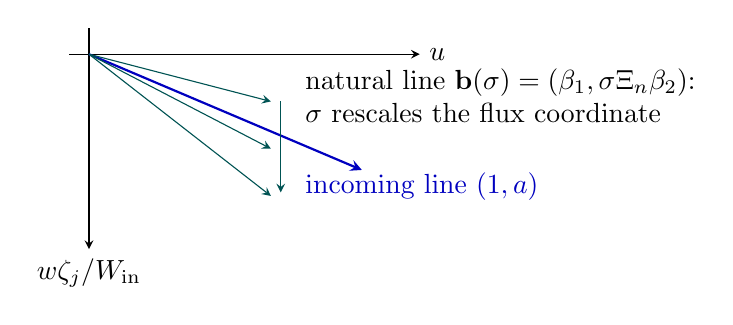
\begin{tikzpicture}[x=2.1cm,y=1.5cm,>=stealth]
\draw[->] (-.12,0)--(2,0) node[right] {$u$};
\draw[->] (0,.22)--(0,-1.65) node[below] {$w\zeta_j/W_{\rm in}$};
\draw[thick,blue!75!black,->] (0,0)--(1.65,-.98);
\node[anchor=west,blue!75!black] at (1.25,-1.12) {incoming line $(1,a)$};
\draw[teal!65!black,->] (0,0)--(1.1,-.4);
\draw[teal!65!black,->] (0,0)--(1.1,-.8);
\draw[teal!65!black,->] (0,0)--(1.1,-1.2);
\draw[->,teal!65!black] (1.16,-.4)--(1.16,-1.17);
\node[anchor=west,align=left] at (1.25,-.35)
 {natural line $\mathbf b(\sigma)=(\beta_1,\sigma\Xi_n\beta_2)$:\\
  $\sigma$ rescales the flux coordinate};
\end{tikzpicture}
\caption{Selection of a height ratio in the plane of boundary states.
The slope of the incoming line lies in a fixed negative interval.
As $\sigma$ varies, the natural line sweeps past it with speed bounded
below, so the two lines are close only for a short interval of
$\sigma$.}
\label{fig:height-selection}
\end{figure}

\begin{lemma}[Simultaneous selection of the heights]
\label{lem:radial-product-selection}
If $N$ is large enough, then at each endpoint the height ratios
$\sigma_n\in[1,2]$, $n\ge N$, can be chosen so that for every $n$ and
every $j\in\mathcal I_n$ the incoming and natural lines at the join
preceding cell $n$ make an angle of sine at least
$\delta_n=c_0e^{-n^2}$ in the state \eqref{eq:rad-eq-js7}.
\end{lemma}

\begin{proof}
The band $\mathcal I_n$ contains at most
$\jn_n=C_*q_ne^{n^2/2}(1+o(1))$ frequencies, so the total length of
the excluded intervals satisfies
\begin{equation}\label{eq:rad-eq-js13}
 \sum_{n\ge N}C\,\#\mathcal I_n\,\delta_n
 \le C\,C_*c_0\sum_{n\ge N}q_n\,e^{-n^2/2}<\frac12
\end{equation}
for large $N$. The excluded interval for a pair $(n,j)$ depends on
the ratios $\sigma_k$ with $k\ne n$, but the bound for its length does
not, and this is all we need.

Consider first finitely many bands $N\le n\le N_1$, with
$\sigma_k=1$ for $k>N_1$, and Lebesgue measure on the cube
$[1,2]^{N_1-N+1}$. By Fubini's theorem and the uniform
one-dimensional bound, the set of ratios violating the condition for a
given pair $(n,j)$ has measure at most $C\delta_n$, and by
\eqref{eq:rad-eq-js13} the union of these sets has measure less than
one. So a good choice exists for every $N_1$. Extend each of these
choices by ones and pass to a subsequence converging in every
coordinate. For a fixed frequency, the transfer across finitely many
cells is continuous in the ratios, and the natural line is continuous
in the product topology by Remark~\ref{rem:line-continuity}. Each
condition on the angle is closed, hence holds for the limit. The two
endpoints are treated independently.
\end{proof}

\subsection{Summary}

We have constructed, at each endpoint, a smooth flat tail with the
following properties, for every even frequency $j$ with band index
$n$: beyond cell $n$ the equation $L_ju=0$ has a unique decaying
solution, which is flat at the endpoint, and $L_j$ has a Dirichlet
inverse with the localized bound \eqref{eq:rad-eq-dj5}; at the
entrance of cell $n$ the natural line makes an angle at least
$\delta_n$ with the line arriving through the preceding positive cap.

We have \emph{not} yet shown that gluing the tails to the central
model preserves the spectral gaps of the pieces. That global question
is the subject of the next section. Its answer uses both halves of the
present construction: the selected angle at the transition cell, and
the strong attenuation through the positive cap that precedes it.

\section{The inverse on the whole annulus}
\label{sec:radial-reference-inverse}

Spectral gaps of the individual pieces do not automatically survive
gluing. A homogeneous solution can leave one piece, return through its
neighbour, and satisfy a new matching condition. We must therefore
solve the matching problem for the whole annulus, not just list the
inverses of the pieces. This section does so and completes the proof
of Proposition~\ref{prop:rad-fixed-theorem}.

\subsection{Overview}

Everything is done one frequency at a time. Fix an even frequency $j$
and let $n$ be its band index, $j\in\mathcal I_n$
(Section~\ref{subsec:bands}). At each end the annulus is divided into
three regions (Figure~\ref{fig:frequency-regions}).
\begin{itemize}
\item The \emph{inner region}: the central model, the cells $m<n$ of
 both tails, and the positive intervals between them. All these
 pieces have large action at the frequency $j$, so each is governed by
 its own spectral inverse, and neighbouring pieces are coupled only
 through exponentially small terms.
\item The \emph{outer core} at each end: the join preceding cell $n$
 and cell $n$ itself. Nothing is small here, but the core is a single
 cell: crossing it costs a known finite factor, and the height
 selection of Lemma~\ref{lem:radial-product-selection} keeps the
 matching angle at its entrance above $\delta_n$.
\item The \emph{deep tail} at each end: the cells $m>n$, governed by
 the recurrence of Lemma~\ref{lem:radial-deep-inverse}.
\end{itemize}
The inverse is assembled in four steps: an inner inverse $G_h$ with
zero boundary values at the two entrances of the outer cores
(Section~\ref{subsec:rad-localized-hilbert-assembly}); an outer inverse
$R_o$ at each end, with the natural condition at the endpoint
(Section~\ref{subsec:outer-inverse}); a $2\times2$ linear system for
the two boundary values that remain, one for each end
(Section~\ref{subsec:terminal-matching}); and weighted estimates for
the resulting formula (Section~\ref{subsec:global-estimate}).

One principle organizes the estimates. A correction created at the
transition cell is large: it costs $\delta_n^{-1}$, the transfer
factor $e^{C_o\tau_{n,j}}$ of the core, and coefficient powers. If its
output stays in cell $n$ or beyond, this cost is absorbed by the
coefficient weight allowed in the output norm there. If its output
returns to the interior, it must first cross the positive cap
preceding the transition join, which attenuates it by
$e^{-c\tau_{n-1,j}}$; and $\tau_{n-1,j}/\tau_{n,j}\asymp e^{n}$, so the
attenuation wins.

\begin{figure}[htbp]
\centering
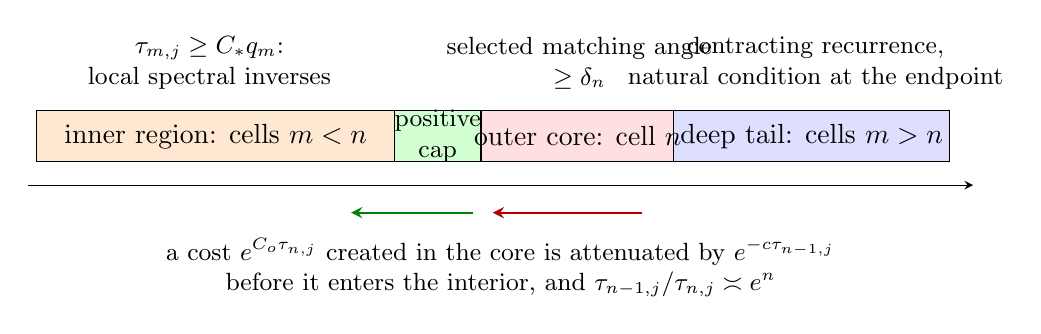
\begin{tikzpicture}[x=1cm,y=1cm,>=stealth]
\draw[->] (0,0)--(12,0);
\draw[fill=orange!18] (.1,.3) rectangle (4.65,.95);
\draw[fill=green!18] (4.65,.3) rectangle (5.75,.95);
\draw[fill=red!12] (5.75,.3) rectangle (8.2,.95);
\draw[fill=blue!13] (8.2,.3) rectangle (11.7,.95);
\node at (2.38,.62) {inner region: cells $m<n$};
\node[align=center,font=\small] at (5.2,.62) {positive\\cap};
\node at (6.98,.62) {outer core: cell $n$};
\node at (9.95,.62) {deep tail: cells $m>n$};
\node[align=center,font=\small] at (2.3,1.55)
 {$\tau_{m,j}\ge C_*q_m$:\\local spectral inverses};
\node[align=center,font=\small] at (7,1.55)
 {selected matching angle\\$\ge\delta_n$};
\node[align=center,font=\small] at (10,1.55)
 {contracting recurrence,\\natural condition at the endpoint};
\draw[->,thick,red!70!black] (7.8,-.35)--(5.9,-.35);
\draw[->,thick,green!50!black] (5.65,-.35)--(4.1,-.35);
\node[align=center,font=\small] at (6,-1.05)
 {a cost $e^{C_o\tau_{n,j}}$ created in the core is attenuated by
  $e^{-c\tau_{n-1,j}}$\\before it enters the interior, and
  $\tau_{n-1,j}/\tau_{n,j}\asymp e^n$};
\end{tikzpicture}
\caption{The decomposition of one end of the annulus at a frequency
$j\in\mathcal I_n$. The other end is treated at the same time. The
position of the division changes with the frequency; the profile is
chosen once.}
\label{fig:frequency-regions}
\end{figure}

\paragraph{Notation of this section.}
We write $w$ for the profile. Estimates are made in the Hilbert space
$L^2(d\mu)$, $d\mu=\varpi\,dr$, with the conventions
\begin{equation}\label{eq:rad-eq-hn1}
 B_j=-\varpi^{-1}L_j,
 \qquad F=-\varpi^{-1}f,\qquad
 \langle u,F\rangle_{L^2(d\mu)}=-\int\overline u\,f\,dr ,
\end{equation}
so that $L_ju=f$ is the same as $B_ju=F$; we also write
$\mathscr H_j=-L_j$. For a border column $k=-\varpi^{-1}g_0$ the
Hilbert adjoint is $k^*u=-\ell_0u$; so after a change of sign of the
scalar equation the bordered operator is symmetric. This convention is
used in all energy identities below. Finite matrices that act on
boundary values are written in sans-serif type when their letter is
also used for a scale ($\mA,\mB,\mK,\mS$). The letters $\lambda$,
$\Lambda$, $\kappa$, $T$, $D$, $E$ have the local meanings stated in
each subsection.

\subsection{Completing the profile while keeping the seed}
\label{subsec:rad-cone-bump-target-match}

We first finish the construction of the profile, in such a way that
the solution of $L_2\phi=0$ is preserved exactly. The device is to
prescribe the solution and to solve for the profile.

\begin{lemma}[Connectors]\label{lem:connector}
On an interval put $y=\log r$ and $w=re^f$, and let $\phi$ be a
nonvanishing function with logarithmic slope
$\mathsf k=\phi_y/\phi$. Then $L_2\phi=0$ is equivalent to
\begin{equation}\label{eq:rad-eq-sp1}
 f_y=\frac{\mathsf k^2+\mathsf k_y-4}{4-\mathsf k},
 \qquad\text{that is,}\qquad
 1+f_y=\frac{rw'}{w}=\frac{\mathsf k^2-\mathsf k+\mathsf k_y}{4-\mathsf k}.
\end{equation}
\end{lemma}

\begin{proof}
In the variable $y$ the equation $r^2L_2\phi=0$ reads
$w\phi_{yy}+(w_y-w)\phi_y-4w_y\phi=0$. Divide by $w\phi$ and use
$\phi_{yy}/\phi=\mathsf k_y+\mathsf k^2$ and $w_y/w=1+f_y$.
\end{proof}

Thus any function $\mathsf k(y)$ with $\mathsf k<4$ and
$\mathsf k^2-\mathsf k+\mathsf k_y>0$ produces, by integrating first
$f_y$ and then $\phi_y=\mathsf k\phi$, a positive interval together
with a solution of $L_2\phi=0$ on it. For constant $\mathsf k=\pm2$
the right side of \eqref{eq:rad-eq-sp1} is $1$: the interval is a
cone and $\phi=r^{\pm2}$. This is more reliable than interpolating
$w$ and hoping to keep the kernel.

\paragraph{The central side.}
By \eqref{eq:rad-eq-sc2} the logarithmic slope of the central solution
$\phi_0$ tends to $2$ on the left and to $-2$ on the right, with all
derivatives. Cut the central model far out on both sides and
interpolate $\mathsf k$ to the constant $\pm2$ over a unit interval of
$y$, with cutoffs that match all derivatives. Since the right side of
\eqref{eq:rad-eq-sp1} is $1$ at the constant, closeness in $C^1$ gives
$1+f_y\ge\tfrac34$. This \emph{connector} ends in an exact cone on
which $\phi=r^{2}$ (left) or $\phi=r^{-2}$ (right).

\paragraph{The tail side.}
On the auxiliary cone of a tail with selected heights, the natural
solution at frequency two is $C_+r^2+C_-r^{-2}$. At the right tail the
incoming line is spanned by $r^2$, so the nonzero angle of
Lemma~\ref{lem:radial-product-selection} gives $C_-\ne0$; far along
the cone, towards $r=0$, the slope of the natural solution tends to
$-2$. At the left tail the incoming line is $r^{-2}$, hence $C_+\ne0$
and the slope tends to $2$ towards $r=\infty$. In both cases the
natural solution does not vanish far along the cone, and the same
interpolation of $\mathsf k$ connects it to an exact cone on which the
solution is $r^{-2}$ (right tail) or $r^{2}$ (left tail), keeping
$1+f_y\ge\tfrac34$.

\paragraph{Assembly.}
The exact cones on the central side and on the tail side carry the
same solution, $r^{-2}$ on the right and $r^{2}$ on the left. A change
of radius
\begin{equation}\label{eq:rad-eq-ha1}
 \widetilde r=Rr,\qquad \widetilde w(Rr)=R\,w(r)
\end{equation}
preserves $w/r$, the operators $B_j$ and the measure $\varpi\,dr$; it
places each tail at the required radius. A rescaling of the height of
the tail then matches the additive constant of $f$, without changing
homogeneous solutions or travel angles, and a constant multiple of the
tail solution matches its value. Cone segments of arbitrary length may
be left between the connectors.

The result is one smooth profile $w_*$, flat at both endpoints by
Lemma~\ref{lem:tail-flat}, and one function $\phi_*$ with
$L_{2,w_*}\phi_*=0$ which is flat at both endpoints by
Lemma~\ref{lem:radial-deep-inverse}(iii). Only positive intervals were
added, so the negative components and their travel angles are those of
the models; part~(ii) of Proposition~\ref{prop:rad-fixed-theorem}
follows from Section~\ref{subsec:rad-central-singlepoint} and
Lemma~\ref{lem:morse-arithmetic}, with $\gamma_m^{-1}=3\sqrt{d_m}$.
From now on $w=w_*$. It remains to prove that there is no kernel
besides $\phi_*$ and that the inverse satisfies the stated estimates.

\subsection{A tool: cutting a model inside a positive buffer}
\label{subsec:buffer}

The spectral information of Section~\ref{sec:rosen-reference-packet}
concerns models on the whole line, whereas the profile contains only
finite pieces of them. The following lemma says that cutting a model
inside a region where its potential is large and positive changes its
inverse, and its boundary data, by an exponentially small amount. It
is formulated for the Schr\"odinger operator in the model coordinate.

\begin{lemma}[Cutting inside a positive buffer]\label{lem:fence-compression}
Let $H_0=-\partial_X^2+V$ be self-adjoint on a full model, possibly
with a compact symmetric scalar border supported away from the cuts,
and let $\mathcal H$ denote the resulting operator. Assume
$\mathcal H$ is invertible with $\|\mathcal H^{-1}\|\le B_0$. Let
there be one or two cuts $c_i$, and at each cut numbers $m_i>0$ and
$\Sigma_i>0$ such that
\begin{itemize}
\item $V\ge m_i^2$ on the exterior of the cut and on the inward
 interval of length $(\Sigma_i+6)/m_i$ adjacent to it (the
 \emph{buffer});
\item $V\le Cm_i^2$ on two layers of width $4/m_i$: one at the cut and
 one at the inner end of the buffer;
\item an exterior wall, if there is one, is at distance at least
 $4/m_i$ from the cut.
\end{itemize}
Let $\alpha_i^{\rm in}$ be the least energy
$\int(|v'|^2+V|v|^2)\,dX$ of a function on the buffer with $v=1$ at
the cut and $v=0$ at the inner end of the buffer, and
$\alpha_i^{\rm out}$ the least energy of a function on the exterior
with $v=1$ at the cut. Then
$\alpha_i^{\rm in},\alpha_i^{\rm out}\asymp m_i$. Put
$D=\diag(\alpha_i^{\rm in}+\alpha_i^{\rm out})$.

Let $\mathcal H_D$ be the operator on the retained interval with the
Dirichlet condition at the cuts; let $T$ be its Poisson map, which
sends boundary values at the cuts to the homogeneous solution with
zero scalar equation; and let $\Lambda$ be its matrix of outward
derivatives at the cuts. If $B_0m_i^2e^{-\Sigma_i}$ is sufficiently
small at every cut, then
\begin{equation}\label{eq:buffer-estimates-new}
 \begin{gathered}
 \|\mathcal H_D^{-1}\|\le B_0+C\sum_i m_i^{-2},\qquad
 \|TD^{-1/2}\|\le C\Bigl(\sum_i m_i^{-2}\Bigr)^{1/2},\\
 D^{-1/2}\bigl(\Lambda-\diag\alpha_i^{\rm in}\bigr)D^{-1/2}
       =O(E),\qquad
 |E_{ik}|\le CB_0\,m_im_k\,e^{-\Sigma_i-\Sigma_k}.
 \end{gathered}
\end{equation}
In particular $\Lambda$ is positive definite.
\end{lemma}

In words: the cut model has essentially the inverse of the full model;
a boundary value at a cut penetrates only a distance $1/m_i$; and the
response of the cut model to a boundary value is, up to a doubly
exponentially attenuated error, that of the buffer alone.

\begin{proof}
\step{1: the energies}
Expanding $\int|v'\pm m_iv|^2\ge0$ shows that the energy of a function
with $v=1$ at the cut is at least $m_i$. A test function supported
within distance $2/m_i$ of the cut gives the matching upper bound.

\step{2: an exact Green column at each cut}
Join at the cut the minimizers of the two energies. After division by
$\alpha_i^{\rm in}+\alpha_i^{\rm out}$ this is the Green function, with
pole at the cut, of the operator with a Dirichlet wall at the inner
end of the buffer. Multiply it by a cutoff which vanishes near that
wall, and call the result $K_i$. Comparison with the solutions of
$-v''+m_i^2v=0$ gives
\[
 \mathcal H(K_i,0)=(\delta_{c_i}+f_i,\,0),\qquad
 \|K_i\|_2\le Cm_i^{-3/2},\qquad
 \|f_i\|_2\le Cm_i^{1/2}e^{-\Sigma_i} .
\]
The commutator term $f_i$ is an ordinary $L^2$ function supported in
the inner layer, and the support of the cutoff does not meet the
border. Therefore
\[
 \boldsymbol g_i=(K_i,0)-\mathcal H^{-1}(f_i,0)
\]
satisfies $\mathcal H\boldsymbol g_i=(\delta_{c_i},0)$ exactly.

\step{3: the matrix of cut values}
Let $\Gamma_{ik}$ be the value at $c_i$ of the field component of
$\boldsymbol g_k$. The correction $\mathcal H^{-1}(f_k,0)$ solves the
homogeneous equation in the buffer at $c_i$ and satisfies the exterior
condition, so on its way from the inner layer to the cut it decays by
a further factor $e^{-\Sigma_i}$. Passing from an $L^2$ bound to a
pointwise bound costs $Cm_i^{1/2}$: where $V\ge m_i^2$ the modulus of
this solution is monotone, so its value at a point is at most
$m_i^{1/2}$ times its $L^2$ norm over the preceding interval of length
$1/m_i$. With $\|\mathcal H^{-1}(f_k,0)\|\le
B_0\,Cm_k^{1/2}e^{-\Sigma_k}$ and $D_{ii}\asymp m_i$ this gives
\[
 D^{1/2}\,\Gamma\,D^{1/2}=I+E,\qquad
 |E_{ik}|\le CB_0\,m_im_k\,e^{-\Sigma_i-\Sigma_k} ,
\]
which also follows from Green's identity applied to two of the
commutator terms. Under the smallness assumption this matrix is
invertible.

\step{4: the cut operator}
Let $\iota$ extend a source on the retained interval by zero, let
$\mathcal R$ restrict a field to the retained interval, both keeping
the scalar, and let $\boldsymbol g_I$ be the restricted Green
columns. Subtracting the cut values gives
\[
 \mathcal H_D^{-1}=\mathcal R\,\mathcal H^{-1}\iota
                     -\boldsymbol g_I\,\Gamma^{-1}\boldsymbol g_I^*,
 \qquad T=\boldsymbol g_I\,\Gamma^{-1}.
\]
There is no hidden kernel: a homogeneous solution with zero values at
the cuts, extended by zero, solves the full equation with delta
sources at the cuts, and the invertibility of $\Gamma$ forces their
coefficients to vanish. Moreover
\[
 \|\boldsymbol g_i\|\,D_{ii}^{1/2}
 \le C\bigl(m_i^{-1}+B_0\,m_i\,e^{-\Sigma_i}\bigr)\le Cm_i^{-1},
\]
which gives the first two bounds in
\eqref{eq:buffer-estimates-new}. Finally, the interior and exterior
derivatives of a Green column add up to the coefficient of its delta
function, so
$\Lambda=\Gamma^{-1}-\diag\alpha_i^{\rm out}$; this proves the third
bound and the positivity. The symmetric border cancels in all the
Green identities used.
\end{proof}

\paragraph{Translation to radial quantities.}
Lemma~\ref{lem:fence-compression} is applied to the models through the
dictionary of Lemma~\ref{lem:liouville}. For $u=\mathcal P^{-1/2}\psi$,
\begin{equation}\label{eq:rad-eq-hn2}
 \|u\|_{L^2(d\mu)}^2=12\lambda\int\upsilon^2|\psi|^2\,dX,
 \qquad wu_r=\lambda\sqrt{\mathcal P}
       \Bigl(\psi_X-\frac{\mathcal P_X}{2\mathcal P}\,\psi\Bigr),
\end{equation}
where $\upsilon=r_X/r$; working with $\sqrt\lambda\,\psi$ removes the
height $\lambda$ from all formulas. The quantity $m_i$ of the lemma is
$\sqrt V=j\sqrt{|\rho|}$ in the buffer. For the two caps of a Morse
cell $m$, with $\Delta X$ the length available for the buffer,
\[
 (m_i,\ \Delta X,\ \upsilon)\asymp
 \bigl(j\sqrt{A_m},\ 1,\ A_m\bigr)\ \text{(short cap)},\qquad
 \bigl(jA_m^{9/2},\ A_m^{-4},\ A_m^5\bigr)\ \text{(long cap)}.
\]
In both cases the buffer has action $\Sigma_i=c\,\tau_{m,j}$, with
$\tau_{m,j}=j\sqrt{A_m}$ as in \eqref{eq:cap-action}, and
$\upsilon/m_i\le C/j$. The inverse of the full Morse model costs a
coefficient power, by \eqref{eq:rad-eq-rm1}. For the central model, a
cut at $|X|=X_0$ has $m_i\asymp jX_0$ and action $c\,jX_0^2$, and the
weighted inverse of the full model is bounded by
Lemma~\ref{lem:central-weighted}.

By the second formula in \eqref{eq:rad-eq-hn2}, the Liouville factor
contributes to the radial flux. At the cuts of the central model, with
$\epsilon_i=\pm1$ the outward sign and $\mathcal P_i$ the value of
$\mathcal P$ at the cut, the matrix of outward radial fluxes is
\begin{equation}\label{eq:rad-eq-hn3}
 \Lambda_r=\lambda\,\diag(\sqrt{\mathcal P_i})\,
                  \Lambda\,\diag(\sqrt{\mathcal P_i})
          +\lambda\,a_c\,\diag(\epsilon_i\mathcal P_i).
\end{equation}
Its leading diagonal part is therefore
\begin{equation}\label{eq:kappa-def}
 \kappa_i=\lambda\,\mathcal P_i\,(\alpha_i^{\rm in}+\epsilon_ia_c),
\end{equation}
which is positive and comparable to $\lambda\mathcal P_im_i$ at far
cuts. For a Morse cell $\mathcal P=1$ and
$\kappa_i=\lambda\alpha_i^{\rm in}$. The term with $a_c$ must be kept
for the fluxes to match exactly.

\subsection{The inner region}
\label{subsec:rad-localized-hilbert-assembly}

Fix $j\in\mathcal I_n$. The inner domain consists of the central
model, the cells $m<n$ of both tails, and the positive intervals
between them; its two outer boundary points are the entrances of the
joins that precede cell $n$ at the two ends. We impose zero boundary
values there. At $j=2$ the central model carries its temporary border.

\paragraph{Decomposition.}
Cut each model inside its positive caps, at points to which
Lemma~\ref{lem:fence-compression} applies. The inner domain is then
the union of the cut models and of the \emph{gaps} between them; a gap
consists of the outer parts of two caps and of the join, connector or
cone between them, and is a positive interval. On every gap the
quadratic form of $\mathscr H_j$ is coercive:
\begin{equation}\label{eq:rad-eq-hn5}
 Q_j(u)=\int\Bigl(w|u_r|^2+j^2\,\frac{w'}r\,|u|^2\Bigr)\,dr
               \ge c\,j^2\,\|u\|_{L^2(d\mu)}^2 ,
\end{equation}
with $c=\tfrac16$ on the joins, where $rw'/w\ge2$ by
\eqref{eq:join-slope}, and a smaller fixed $c$ on cone heads and on
the connectors of the central model. Consequently the Poisson map
$P_C$ of a gap and its matrix $\Lambda_C$ of outward fluxes satisfy
$\|P_Ca\|\le(C/j)\,(a^*\Lambda_Ca)^{1/2}$.

Let $D_h$ be the direct sum of the Dirichlet inverses of the cut
models and of the gaps. Let $T_h$ map values at the cuts to the
function which is homogeneous on every cut model and every gap with
these values (and zero scalar equation). At the cuts define
\begin{equation}\label{eq:rad-eq-hn6}
 \mS_0=\diag(\kappa_i)+\bigoplus_C\Lambda_C,
 \qquad \mS=\mS_0+E_h ,
\end{equation}
where $\mS$ is the matrix of total outward fluxes of $T_h$, and $E_h$
collects the errors of Lemma~\ref{lem:fence-compression}. A short gap
can have a large off-diagonal entry in $\Lambda_C$; this entry is kept
in $\mS_0$ and is not treated as an error. The matrix $\mS_0$ is
positive, consists of blocks of size at most two, and dominates
$D_\kappa=\diag(\kappa_i)$. A zero-boundary solution with source $F$
has outgoing flux $-T_h^*F$ at the cuts, and matching values and
fluxes gives the exact inner inverse
\begin{equation}\label{eq:rad-eq-hn9}
 G_h=D_h+T_h\,\mS^{-1}\,T_h^* ,
\end{equation}
provided $\mS$ is invertible.

\paragraph{Weights.}
To obtain estimates which are uniform in the number of cells, and
which carry the weights of
Proposition~\ref{prop:rad-fixed-theorem}, let $W$ be a positive
function equal to one on the finite middle part and of size
\begin{equation}\label{eq:rad-eq-hn4}
 W_m=\Bigl(\frac{\mathcal E_m}{\mathcal E_N}\Bigr)^{\ea}
     \Bigl(\frac{H_m}{H_N}\Bigr)^{-\gamma}
\end{equation}
on cell $m$. We take $W$ constant on each gap, equal to the geometric
mean of the two neighbouring values, and let it vary inside the
cells. For $|\gamma|\le1$,
\begin{equation}\label{eq:adjacent-weight-ratio-new}
 \Bigl|\log\frac{W_{m+1}}{W_m}\Bigr|
 \le Cm^2+C\,\ea\,m^{3/2}\log(e+m),
\end{equation}
so this choice changes the norms on each cell by coefficient powers
only. Let $\Omega=\diag(W(c_i))$ be the weights at the cuts. Since
the two ends of a gap have the same weight, $\Omega$ commutes with
$\mS_0$.

\paragraph{Smallness of the coupling.}
By Lemma~\ref{lem:fence-compression} and \eqref{eq:rad-eq-hn2}, the
errors $E_h$, normalized by $\kappa_i^{1/2}$ on both sides and
conjugated by the weights, are bounded by
\begin{equation}\label{eq:rad-eq-hn7}
 \mathcal E_m^{C(\ea)}\langle j\rangle^C e^{-c\tau_{m,j}},\qquad
 C\langle j,X_0\rangle^Ce^{-cjX_0^2},\qquad
 C_N\langle j\rangle^Ce^{-cjL}
\end{equation}
for a cell $m<n$, for the central cuts at $|X|=X_0$, and for a cone
head of length $L$ in $\log r$, respectively. The Poisson function of
a model cut has a leading part of norm at most
$(C/j)\sqrt{\kappa_i}\,|a_i|$ in $L^2(d\mu)$, because
$\upsilon/m_i\le C/j$, and a remainder bounded by the first quantity
in \eqref{eq:rad-eq-hn7}.

These bounds have to be small uniformly over all frequencies of all
bands beyond $m$, that is, for all $j$ with
$t:=\tau_{m,j}\ge C_*q_m$, however large. Since
$\log\langle j\rangle\le\log(1+t)+Cm^2$, the logarithm of the first
quantity in \eqref{eq:rad-eq-hn7} is at most
\begin{equation}\label{eq:inner-uniform-suppression}
 c_1\,q_m+c_2\log(1+t)-c_3t
 \le c_1\,q_m-\tfrac34c_3t+C
 \le-\tfrac12c_3t+C
 \qquad\text{if }C_*\ge4c_1/c_3,
\end{equation}
with fixed $c_1,c_2,c_3>0$; here $m^2=o(q_m)$ was absorbed in $c_1$, and
$c_2\log(1+t)\le c_3t/4+C$. So after $C_*$ is fixed, increasing $N$
makes these errors smaller than any prescribed tolerance,
simultaneously for all $m<n$ and all admissible $j$. The other two
quantities in \eqref{eq:rad-eq-hn7} are made small by the choice of
the central cuts and of the lengths of the cone heads. The constants
are thus chosen in the order
\begin{equation}\label{eq:order-of-constants}
 \ea\ \longrightarrow\ C_*\ \longrightarrow\ N\ \longrightarrow\
 X_0,\ L .
\end{equation}

\begin{lemma}[The inner inverse]\label{lem:inner-inverse}
With the choices \eqref{eq:order-of-constants}, for both signs,
\begin{equation}\label{eq:rad-eq-hn8}
 \bigl\|\mS_0^{-1/2}\,\Omega^{\pm1}E_h\,\Omega^{\mp1}\mS_0^{-1/2}\bigr\|
 <\tfrac12,
 \qquad
 \bigl\|W^{\pm1}\,T_h\,\Omega^{\mp1}\mS_0^{-1/2}\bigr\|\le\frac Cj .
\end{equation}
Hence $\mS$ is invertible, \eqref{eq:rad-eq-hn9} is a two-sided
inverse of the inner problem, and there is a fixed exponent $\el$ such
that, with $W_1=W\,(\mathcal E/\mathcal E_N)^{-\el}$,
\begin{equation}\label{eq:inner-inverse-estimates-new}
 \|W_1\,G_h\,W^{-1}\|\le C,\qquad
 \|W^{\pm1}\,G_h\,W^{\mp1}\|\le\mathcal E_n^C .
\end{equation}
\end{lemma}

\begin{proof}
For the first bound in \eqref{eq:rad-eq-hn8}, normalize the error of
each model by $\kappa_i^{1/2}$ at its two cuts. Every cut belongs to
at most two such blocks, so their sum has norm at most twice the
largest of their norms, and $\|\mS_0^{-1/2}D_\kappa^{1/2}\|\le1$ on
both sides.
For the second, consider the Poisson function of one model cut, with
boundary value $u_i$. In the model coordinate
\eqref{eq:buffer-estimates-new} gives
$\|\psi\|_{L^2(dX)}\le Cm_i^{-1}D_{ii}^{1/2}|\psi_i|$, and by
\eqref{eq:rad-eq-hn2} and \eqref{eq:kappa-def} this is
$\|u\|_{L^2(d\mu)}\le C(\upsilon/m_i)\sqrt{\kappa_i}\,|u_i|
\le(C/j)\sqrt{\kappa_i}\,|u_i|$ for the part of the function in the
buffer; the rest is bounded by \eqref{eq:rad-eq-hn7}. Now sum the
squares of the norms of the local Poisson functions over the cut
models, which are disjoint, and over the gaps, which have bounded
overlap with them. Both estimates are independent of the number of
cells.

They give the inverse as follows. Since $\Omega$ commutes with
$\mS_0$,
\[
 \Omega^{\pm1}\mS^{-1}\Omega^{\mp1}
 =\mS_0^{-1/2}\bigl(I+\mS_0^{-1/2}\Omega^{\pm1}E_h\Omega^{\mp1}
   \mS_0^{-1/2}\bigr)^{-1}\mS_0^{-1/2},
\]
and the middle factor has norm at most $2$. Hence, using
\eqref{eq:rad-eq-hn8} with both signs,
\[
 \bigl\|W^{\pm1}\,T_h\mS^{-1}T_h^*\,W^{\mp1}\bigr\|
 \le2\,\bigl\|W^{\pm1}T_h\Omega^{\mp1}\mS_0^{-1/2}\bigr\|\,
       \bigl\|\mS_0^{-1/2}\Omega^{\pm1}T_h^*W^{\mp1}\bigr\|
 \le\frac{C}{j^2} .
\]
So the coupling term of \eqref{eq:rad-eq-hn9} loses nothing. The
Dirichlet inverses in $D_h$ cost
coefficient powers of their own cells, which is the loss $\el$ in the
first bound of \eqref{eq:inner-inverse-estimates-new}; in the second
bound all cells are estimated by the largest one. The invertibility of
the Dirichlet blocks and of $\mS$ gives both inverse identities, and
the symmetry of $G_h$ is the corresponding Green identity.
\end{proof}

The first estimate in \eqref{eq:inner-inverse-estimates-new} is
localized: an inner source in cell $m$ produces an output which is
controlled with the weight of cell $m$, up to the loss $\el$. It will
handle ordinary inner sources. The second, coarser estimate will be
applied only to boundary terms which already carry an exponentially
small factor.

\subsection{The outer region: an inverse without division by a boundary value}
\label{subsec:outer-inverse}

Fix an end. The outer region consists of the \emph{outer core}, namely
the join preceding cell $n$ and cell $n$, and of the deep tail beyond
it. The large positive cap before the join belongs to the inner
region. At the right end the deep tail begins with a mass interval, at
the left end with an initial resistance edge
(Section~\ref{subsec:exact-reduction}). Let $r_o$ be a radial
coordinate increasing outward, and choose a scale $\lambda>0$ with
$e^{-Cn^2}\le\lambda/\lambda_n\le e^{Cn^2}$. We describe solutions on
the core by the state $(u,z)$ with $z=wu_{r_o}/\lambda$.

\begin{lemma}[Inputs from the core and the deep tail]
\label{lem:transition-inputs}
Let $\mathsf T_{\rm core}$ be the transfer matrix of $L_ju=0$ across
the core in the state $(u,z)$, and let $P_d$ be the natural solution
on the deep tail with value one at its entrance. Then
\begin{equation}\label{eq:transition-inputs-new}
 \begin{gathered}
 \|\mathsf T_{\rm core}\|+\|\mathsf T_{\rm core}^{-1}\|
 \le\mathcal K_n:=e^{Cn^2+C_o\tau_{n,j}},
 \qquad \int_{\rm core}\varpi\,dr_o\le\lambda\,e^{Cn^2},\\
 \|P_d\|_{L^2(d\mu)}\le\sqrt\lambda\,e^{Cn^2},
 \qquad \|B_{d,D}^{-1}\|\le Cj^{-4},
 \end{gathered}
\end{equation}
where $B_{d,D}$ is $B_j$ on the deep tail with the Dirichlet condition
at its entrance.
\end{lemma}

\begin{proof}
The last bound is \eqref{eq:rad-eq-rm20}. The mass of the core is
$12\lambda_n\int(r_X/r)^2\,dX$ plus the negligible mass of the join,
and is estimated by \eqref{eq:rad-eq-rm6}. The contraction
\eqref{eq:rad-eq-dg4} bounds $\|P_d\|^2$ by a constant times the
first mass of the deep tail; if an initial resistance edge comes
first, the value at the next mass entrance is at most
$C/(\Lambda\mu R_0)$ and the mass of the edge is small, with the same
conclusion.

For the transfer matrix, consider first a positive piece. In the
state $(u,z)$ the equation is $u_{r_o}=(\lambda/w)\,z$,
$z_{r_o}=(j^2w_r/(\lambda r))\,u$. Replace $z$ by $\varsigma z$ with
a constant $\varsigma>0$ and apply Gronwall's inequality; the best
choice of $\varsigma$ balances the integrals of the two coefficients,
and $\varsigma^{\pm1}\le e^{Cn^2}$ on the pieces of the core. This
bounds the transfer in either direction by
\[
 e^{Cn^2}\exp\biggl(2j\sqrt{\int\frac{dr_o}{w}\,
                                  \int\frac{w_r}{r}\,dr_o}\,\biggr).
\]
The product under the square root is $O(A_n)$ on each cap, by
Lemma~\ref{lem:cell}, and smaller on the join. On the negative
component use $u_{XX}+j^2\rho\,u=0$ and the energy
$\mathsf e=|u_X|^2+(1+j^2\rho)|u|^2$, which satisfies
\[
 |\mathsf e_X|\le\Bigl[1+\frac{j^2|\rho_X|}{1+j^2\rho}\Bigr]\mathsf e .
\]
The component has length $O(n^2)$ in $X$ and $\rho$ has a single
maximum, so the integral of the second term is at most
$2\log(1+j^2\max\rho)$. Converting between $(u,u_X)$ and $(u,z)$ costs
$e^{Cn^2}$.
\end{proof}

\paragraph{A Robin inverse.}
Let $V$ be the natural solution on the outer region. Its value at the
entrance $r_{o,-}$ of the core may vanish, so we do not divide by it.
Instead normalize its full state there, and let $U$ be the solution
with the perpendicular state:
\begin{equation}\label{eq:rad-eq-tm1}
 v=\Bigl(V,\ \frac{f_V}{\lambda}\Bigr)(r_{o,-}),\quad |v|=1,
 \qquad f_u:=wu_{r_o},
 \qquad \Bigl(U,\ \frac{f_U}{\lambda}\Bigr)(r_{o,-})=v^\perp:=(-v_2,v_1).
\end{equation}
Then $w\,(UV_{r_o}-U_{r_o}V)=-\lambda$, and the kernel
\[
 K_o(r_o,t_o)=\lambda^{-1}\,U(\min(r_o,t_o))\,V(\max(r_o,t_o))
\]
defines operators
\begin{equation}\label{eq:outer-robin-new}
 R_oF=\int K_o(r_o,t_o)\,F(t_o)\,d\mu(t_o),\qquad
 G_of=-\int K_o(r_o,t_o)\,f(t_o)\,dt_o ,
\end{equation}
which invert $B_j$ in $L^2(d\mu)$ and $L_j$ for the pairing $dr_o$,
respectively, with the natural condition at the endpoint and the
Robin condition $v\cdot(u,f_u/\lambda)=0$ at the entrance. For a
solution $u=R_oF$, Green's identity with $V$ gives the complementary
boundary quantity,
\begin{equation}\label{eq:rad-eq-tm2}
 v^\perp\cdot\Bigl(u,\ \frac{f_u}{\lambda}\Bigr)(r_{o,-})
       =\frac1\lambda\int V\,\varpi\,F\,dr_o,
 \qquad \|V\|_{L^2(d\mu)}\le\sqrt\lambda\,\mathcal E_n^C\,\mathcal K_n ;
\end{equation}
the boundary term at the endpoint vanishes by
Section~\ref{subsec:deep-green}.

\begin{lemma}[The outer inverse]\label{lem:outer-inverse}
The operator $R_o$ satisfies
\begin{equation}\label{eq:rad-eq-tm3}
 \|R_o\|\le\mathcal E_n^C\,\mathcal K_n^2 ,
\end{equation}
and, for the localizations $\vartheta_k,\vartheta_m$ to cells
$k,m\ge n-O(1)$,
\begin{equation}\label{eq:rad-eq-tm4}
 \|\vartheta_k\,R_o\,\vartheta_m\|
 \le\mathcal E_k^C\,\mathcal E_m^C\,\mathcal K_n^2\,e^{-|S_k-S_m|}.
\end{equation}
The same bounds hold for $G_o$ between the spaces $L^2(dr_o)$.
\end{lemma}

\begin{proof}
The factor $\lambda^{-1}$ in $K_o$ causes no loss. On the core it is
cancelled by the mass bound in \eqref{eq:transition-inputs-new}. On
the deep tail, restricting the kernel gives exactly
\[
 (R_o)_{d,d}=B_{d,D}^{-1}+P_d\,K_o(r_{o,+},r_{o,+})\,P_d^*,
 \qquad |K_o(r_{o,+},r_{o,+})|
        \le\lambda^{-1}\,\mathcal E_n^C\,\mathcal K_n^2 ,
\]
where $r_{o,+}$ is the entrance of the deep tail, and the two factors
$P_d$ cancel $\lambda^{-1}$. The blocks between core and deep tail
contain one factor $P_d$ each. This proves \eqref{eq:rad-eq-tm3}. The
localized bound follows from \eqref{eq:rad-eq-dj5} for the first term
and from \eqref{eq:rad-eq-rm17} for the factors $P_d$: a product of
two such decay factors, both measured from the entrance, is bounded
by $e^{-|S_k-S_m|}$. Passing to $L^2(dr_o)$ multiplies source and
output by $\varpi^{\mp1/2}$ on their cells, which are coefficient
powers.
\end{proof}

\subsection{Matching the two remaining boundary values}
\label{subsec:terminal-matching}

Let $i$ label the two truncation points, where the inner domain meets
the outer core at each end. Put
\[
 \lambda_i=\frac{j^2\,W_{{\rm in},i}}{r_{{\rm in},i}},
\]
with $W_{{\rm in},i}$ and $r_{{\rm in},i}$ the profile and the radius
at that point; its ratio to $\lambda_n$ lies between $e^{-Cn^2}$ and
$e^{Cn^2}$, so Section~\ref{subsec:outer-inverse} applies with
$\lambda=\lambda_i$. We use the normalized boundary coordinates
\[
 x_i=\sqrt{\lambda_i}\,u_i,\qquad z_i=\frac{f_{u,i}}{\sqrt{\lambda_i}} .
\]
In these coordinates the stand-in solution of
Section~\ref{subsec:height-selection}, which vanishes at a cut in the
preceding positive cap, has the ratio of outward flux to value
\[
 d_i=\frac{f_u}{\lambda_iu}=\frac{r\,u_{r_o}}{j^2u}
 \in\bigl(0,\tfrac12\bigr],
 \qquad D_0:=\diag(d_i),
\]
by the estimate proving \eqref{eq:rad-eq-js6}; in the first band
$d_i=1/j$.

\paragraph{The true inner boundary matrix.}
Let $B_h$ be the inner operator in $L^2(d\mu)$, including the
symmetric border, and $\mathsf q_h$ its quadratic form. We compare the
true matrix of normalized outward fluxes of the inner problem with
$D_0$. Take the stand-in solution with boundary value
$\lambda_i^{-1/2}$, multiply it by a cutoff near the inner end of its
cap, and extend it by zero to a field $\mathsf L_i$ on the inner
domain; let $\mathsf F_i=B_h\mathsf L_i$, with zero scalar
component. Separate fixed fractions of the cap are reserved for this
cutoff and for the buffer of the neighbouring model. Positivity and
the commutator formula
\[
 \mathscr H_j(\chi u)-\chi\,\mathscr H_ju
       =-2w\chi'u'-(w\chi')'u
\]
give, for both signs and with $\omega_i$ the constant value of $W$ on
this gap,
\begin{equation}\label{eq:rad-eq-tm6}
 \begin{gathered}
 \|W^{\pm1}\mathsf L_i\|\,\omega_i^{\mp1}
       \le\frac{C\sqrt{d_i}}{j},\qquad
 \|W^{\pm1}\mathsf F_i\|\,\omega_i^{\mp1}
       \le\sqrt{d_i}\;\mathcal E_n^C\,e^{-\Sigma_{b,i}},\\
 \Sigma_{b,i}=c\,\tau_{n-1,j}\quad\text{(in the first band: }
 \Sigma_{b,i}=c\,jL).
 \end{gathered}
\end{equation}
The first bound uses the energy $d_i$ of the stand-in solution and
\eqref{eq:rad-eq-hn5}; the second uses the attenuation up to the
cutoff layer. The two fields $\mathsf L_i$ have disjoint supports,
and their energy matrix is diagonal with entries
$d_i\,(1+O(\mathcal E_n^Ce^{-2\Sigma_{b,i}}))$.

The exact Poisson map of the inner problem is
$P_h=\mathsf L-G_h\mathsf F$, where $\mathsf L$ and $\mathsf F$ have
the columns $\mathsf L_i$ and $\mathsf F_i$. Completing the square in
the quadratic form gives the true matrix of normalized outward fluxes,
\begin{equation}\label{eq:rad-eq-tm7}
 D_b=\mathsf q_h(\mathsf L,\mathsf L)-\mathsf F^*G_h\mathsf F
       =D_0+E_b,
 \qquad |(E_b)_{ik}|\le
     \mathcal E_n^C\,\sqrt{d_id_k}\;e^{-\Sigma_{b,i}-\Sigma_{b,k}} .
\end{equation}
Indeed, $x^*D_bx$ is the energy $\mathsf q_h(P_hx,P_hx)$ of the
homogeneous solution with boundary values $x$. Since
$B_hG_h\mathsf F=\mathsf F$ and $G_h\mathsf Fx$ vanishes at the
boundary, integration by parts gives
\[
 \mathsf q_h(\mathsf Lx,G_h\mathsf Fx)
 =\langle\mathsf Fx,G_h\mathsf Fx\rangle
 =\mathsf q_h(G_h\mathsf Fx,G_h\mathsf Fx) ,
\]
so in the expansion of $\mathsf q_h(\mathsf Lx-G_h\mathsf Fx,
\mathsf Lx-G_h\mathsf Fx)$ the two cross terms cancel one of the two
correction terms. The error $E_b$ consists of $-\mathsf F^*G_h\mathsf F$
and of the deviation of the energy matrix of the fields $\mathsf L_i$
from $D_0$; both are bounded by \eqref{eq:rad-eq-tm6} and the second
estimate in \eqref{eq:inner-inverse-estimates-new}. This is why the
error contains \emph{two} attenuation
factors. The border is symmetric and the fields $\mathsf L_i$ have
zero scalar component, so no scalar term is missing. Any dependence of
the interior on the selected tails enters only through $E_b$.

\paragraph{The matching system.}
Let $v_i$ be the normalized entrance state \eqref{eq:rad-eq-tm1} of
the natural solution $V_i$ at the end $i$, and put
\[
 \mA=\diag(v_{1,i}),\qquad \mB=\diag(v_{2,i}),\qquad
 \mathcal V=\bigl(V_i/\sqrt{\lambda_i}\bigr)_i ,
\]
so that $\mA^2+\mB^2=I$. Let $F_h$ be a source in the inner domain
and $F_o$ a source in the outer regions. The inner solution is
$G_hF_h+P_hx$, where $x$ are its boundary values. The outward flux of
$P_hx$ is $D_bx$, and by Green's identity that of $G_hF_h$, which
vanishes at the boundary, is $-P_h^*F_h$. The outer solution at the
end $i$ is $R_oF_o$ plus a multiple of $V_i$; by
\eqref{eq:rad-eq-tm1} and \eqref{eq:rad-eq-tm2} its normalized state
$(x_i,z_i)$ at the truncation point is
$(\mathcal V^*F_o)_i\,v_i^\perp$ plus a multiple of $v_i$, the
multiple being the coefficient of $V_i/\sqrt{\lambda_i}$ in the outer
solution. Values and fluxes are continuous at the truncation points.
Taking the component along $v_i^\perp$ gives the matching condition,
and the component along $v_i$ shows that the coefficients of the
natural solutions are $\mA x+\mB z$. The complete matching problem is
therefore
\begin{equation}\label{eq:rad-eq-tm8}
 \begin{gathered}
 z=D_bx-P_h^*F_h,\qquad -\mB x+\mA z=\mathcal V^*F_o,\\
 \text{that is,}\qquad
 \mK x=\mathcal V^*F_o+\mA P_h^*F_h,\qquad \mK=\mA(D_0+E_b)-\mB .
 \end{gathered}
\end{equation}

\begin{lemma}[The matching matrix]\label{lem:matching}
After $C_*$, $N$ and the lengths of the cone heads have been chosen
suitably, the matrix $\mK$ is invertible and
$\|\mK^{-1}\|\le C\delta_n^{-1}$, uniformly in $n$ and in
$j\in\mathcal I_n$.
\end{lemma}

\begin{proof}
The diagonal part $\mA D_0-\mB$ of $\mK$ is controlled by the selected
angle. The state used in Lemma~\ref{lem:radial-product-selection} is
$(u,-u\pm f_u/\lambda_i)$ at the truncation point, which differs from
$(u,f_u/\lambda_i)$ by a fixed linear map, and transport across the
join is close to the identity by \eqref{eq:rad-eq-js14}. Hence
\begin{equation}\label{eq:rad-eq-tm9}
 |v_{1,i}d_i-v_{2,i}|
 =\sqrt{1+d_i^2}\;|\sin\angle(v_i,(1,d_i))|
 \ge c\,\delta_n .
\end{equation}
This holds also when $v_{1,i}=0$. The direction $(1,d_i)$ was fixed
before the height ratio was varied. It therefore suffices to have
\begin{equation}\label{eq:rad-eq-tm10}
 \delta_n^{-1}\|E_b\|<\frac c4,
 \qquad\text{and we also arrange}\qquad
 \mathcal E_n^C\,\delta_n^{-1}\,
     e^{C_o\tau_{n,j}-c\tau_{n-1,j}}<\frac14
\end{equation}
for use in Section~\ref{subsec:global-estimate}. Both hold because
\[
 \frac{\tau_{n-1,j}}{\tau_{n,j}}\asymp e^n,\qquad
 \tau_{n-1,j}\ge C_*q_{n-1},\qquad
 \frac{q_n}{q_{n-1}}\to1,\qquad \frac{n^2}{q_{n-1}}\to0 .
\]
The first relation absorbs $C_o\tau_{n,j}$ into a quarter of
$c\tau_{n-1,j}$, and the others absorb $Cq_n+n^2+|\log c_0|$ into
another quarter, provided $C_*$ is chosen after the coefficient
exponent $C$ and $N$ is large. The first inequality in
\eqref{eq:rad-eq-tm10} even has two attenuation factors, by
\eqref{eq:rad-eq-tm7}. In the first band the role of $\tau_{n-1,j}$ is
played by $jL$, and the length $L$ of the cone heads is taken large.
\end{proof}

\subsection{The matched inverse and its weighted bound}
\label{subsec:global-estimate}

Put $\mK_1=\mA+\mB D_b$. Solving \eqref{eq:rad-eq-tm8} and
reconstructing the coefficient of the natural solution in the outer
regions, which is $\mK_1x-\mB P_h^*F_h$, gives the inverse for the
frequency $j$ on the whole annulus,
\begin{equation}\label{eq:rad-eq-tm11}
 G=\begin{pmatrix}G_h&0\\0&R_o\end{pmatrix}
  +\begin{pmatrix}P_h&0\\0&\mathcal V\end{pmatrix}
   \begin{pmatrix}
       \mK^{-1}\mA&\mK^{-1}\\\mK^{-T}&\mK_1\mK^{-1}
   \end{pmatrix}
   \begin{pmatrix}P_h^*&0\\0&\mathcal V^*\end{pmatrix},
\end{equation}
in the decomposition into inner and outer sources and fields. Since
$D_b$ is symmetric and $\mA,\mB$ are commuting diagonal matrices with
$\mA^2+\mB^2=I$, direct multiplication gives
\[
 \mK\mA=\mA\mK^T,\qquad \mK^T\mK_1=\mK_1^T\mK,\qquad
 \mK_1\mK^{-1}\mA-\mB=\mK^{-T}.
\]
These identities prove the formula and show that the middle matrix is
symmetric; its norm is $O(\delta_n^{-1})$ by Lemma~\ref{lem:matching}.
The boundary weights at the two ends are taken equal, which is
possible because the band index is the same at both ends.

We now prove that $G$ is bounded between the weighted spaces. The
direct terms $G_h$ and $R_o$ are covered by
Lemmas~\ref{lem:inner-inverse} and~\ref{lem:outer-inverse}. The
correction terms are of two kinds, according to where their output
lies, and each kind is paid for in its own way.

\begin{proposition}[Weighted bound at one frequency]
\label{prop:global-reference-bound}
For every compact interval $[\gamma_-,\gamma_+]\subset(0,1)$ there are
exponents $\ea$, $\el>\ea$ and choices of $C_*$, $N$, $X_0$, $L$ such
that, with the weights $W$ of \eqref{eq:rad-eq-hn4} and
$W_1=W\,(\mathcal E/\mathcal E_N)^{-\el}$,
\begin{equation}\label{eq:global-reference-bound-new}
 \|W_1\,G\,W^{-1}\|\le C
\end{equation}
for all even $j\ge2$ and all $\gamma\in[\gamma_-,\gamma_+]$, where at
$j=2$ the temporary border is included. The same bound holds between
the spaces of source densities for $dr$ and fields in $L^2(dr)$, after
an adjustment of the exponents.
\end{proposition}

\begin{proof}
\step{1: terms whose source and output are both outer}
These are the terms of \eqref{eq:rad-eq-tm11} built from $R_o$,
$\mathcal V$ and the leading parts $\mathsf L$ of $P_h$; their sources
and outputs lie in cells of index at least $n-O(1)$. By
\eqref{eq:rad-eq-tm4} and $\|\mK^{-1}\|\le C\delta_n^{-1}$, with fixed
constants $\alpha_1,\alpha_2$,
\[
 \|\vartheta_k\,G_{\rm out}\,\vartheta_m\|
 \le C\exp\{\alpha_1\,(q_k+q_m)+\alpha_2\,q_n-|S_k-S_m|\} ;
\]
here $\alpha_2$ accounts for the cost of the core, since
$\delta_n^{-1}e^{C_o\tau_{n,j}}\le c_0^{-1}\exp(n^2+C_oC_*q_n)$. The
output is outer, so $q_n\le c_1q_k+C_1$; put $\alpha_3=\alpha_2c_1$. Conjugating
by the weights gives, with $\Delta S=S_k-S_m$,
\begin{equation}\label{eq:outer-weighted-block}
 \begin{aligned}
 \log\|\vartheta_k\,W_1G_{\rm out}W^{-1}\vartheta_m\|
 &\le C-(\el-2\alpha_1-\alpha_3)\,q_k\\
 &\quad +(\alpha_1-\ea)\,(q_m-q_k)-|\Delta S|+\gamma\,\Delta S .
 \end{aligned}
\end{equation}
Choose $\el>\max(\ea,2\alpha_1+\alpha_3)$; this is done after $C_*$. Since $q_n$
varies slowly compared with $S_n$,
\[
 |q_m-q_k|\le\varepsilon\,|S_m-S_k|+C_\varepsilon,
 \qquad
 \varepsilon=\frac{1-\gamma_+}{2\,(1+|\alpha_1-\ea|)},
\]
and \eqref{eq:outer-weighted-block} is at most
$C_\gamma-\tfrac12(1-\gamma_+)\,|S_k-S_m|$. With
$s_0=\inf_m(S_{m+1}-S_m)>0$ and $\eta=\tfrac12(1-\gamma_+)$,
\[
 \sup_k\sum_m e^{-\eta|S_k-S_m|}\le1+\frac2{e^{\eta s_0}-1},
\]
and the same holds with $k$ and $m$ exchanged. Schur's test for block
kernels, with the bounded overlap of the localizers and the two ends,
bounds this part of $W_1GW^{-1}$. Note that raising the output
exponent $\el$ helps precisely because the output index $k$ is at
least about $n$; it would not help for an output at a fixed place in
the interior.

\step{2: terms whose output returns to the interior}
The upper right block of \eqref{eq:rad-eq-tm11} is
$P_h\mK^{-1}\mathcal V^*$, and with $P_h=\mathsf L-G_h\mathsf F$ the
part of it which reaches the interior is
\[
 C_{ho}=-(G_h\mathsf F)\,\mK^{-1}\,\mathcal V^* .
\]
Let $\Omega$ be the common weight at the two truncation points, and
$W_h,W_o$ the restrictions of $W$ to the inner and outer regions.
Three bounds are available:
\begin{equation}\label{eq:boundary-column-weights}
 \begin{gathered}
 \|W_h\,G_h\mathsf F\,\Omega^{-1}\|
       \le\mathcal E_n^{C_1}\,e^{-c\tau_{n-1,j}},\\
 \|\Omega\,\mK^{-1}\,\Omega^{-1}\|\le C\delta_n^{-1},\\
 \|\Omega\,\mathcal V^*\,W_o^{-1}\|
       =\|W_o^{-1}\,\mathcal V\,\Omega\|
       \le C_\gamma\,\mathcal E_n^{C_2}\,e^{C_o\tau_{n,j}} .
 \end{gathered}
\end{equation}
The first is the second bound of
\eqref{eq:inner-inverse-estimates-new} applied to
\eqref{eq:rad-eq-tm6}, with $d_i\le\tfrac12$. The second uses that the
weights at the two ends are equal. For the third, the part of the
column $\mathcal V$ in cell $k$ is bounded by
$\mathcal E_n^C\mathcal E_k^C\,e^{C_o\tau_{n,j}}\,e^{-(S_k-S_n)}$;
multiplying by either power of the weight changes the exponent by
$(C\pm\ea)(q_k-q_n)-(1\mp\gamma)(S_k-S_n)$, and the slow variation of
$q$ used in Step~1 makes the sum of the squares finite, leaving a
coefficient power at $n$ and a constant $C_\gamma$. The same argument
gives the version with the reciprocal weights. Multiplying the three
bounds,
\begin{equation}\label{eq:one-boundary-cross-block}
 \|W_h\,C_{ho}\,W_o^{-1}\|
 \le C_\gamma\,\mathcal E_n^C\,\delta_n^{-1}\,
             e^{C_o\tau_{n,j}-c\tau_{n-1,j}}
 \le C_\gamma\,e^{-c\tau_{n-1,j}/2}\le C_\gamma ,
\end{equation}
by the second inequality in \eqref{eq:rad-eq-tm10}, with the constants
there enlarged before $C_*$ and $N$ are chosen; in the first band
$c\,\tau_{n-1,j}$ is replaced by $c\,jL$. Since
$\mathcal E/\mathcal E_N\ge1$ on the tails and is bounded below on the
middle part, $W_1\le C\,W$, which gives the bound with the output
weight $W_1$. The transposed block is treated with the opposite sign
of the weight in \eqref{eq:boundary-column-weights}. Terms with two
columns $G_h\mathsf F$ carry two attenuation factors, and terms with
one such column and one leading part $\mathsf L$ are estimated in the
same way.

\step{3: conclusion}
All terms of \eqref{eq:rad-eq-tm11} have been covered. The passage
between $L^2(d\mu)$ and the spaces for $dr$ costs coefficient powers
on each cell, which are absorbed by enlarging $\ea$ and $\el$.
\end{proof}

\begin{lemma}[One geometry for all exponents]
\label{lem:radial-uniform-exponents}
The profile, the height ratios, the central cuts and the lengths of
the cone heads can be chosen once, so that
\eqref{eq:global-reference-bound-new} holds for every compact interval
$[\gamma_-,\gamma_+]\subset(0,1)$. Only the constants and the
exponents $\ea,\el$ depend on the interval.
\end{lemma}

\begin{proof}
All the finite matching problems, that is the inversion of $\mS$ and
of $\mK$, involve the weights only through the ratios of neighbouring
weights, and \eqref{eq:adjacent-weight-ratio-new} is uniform for
$|\gamma|\le1$. Fix one exponent $\ea$ large enough for the
conversion of sources, and choose $C_*$, $N$, the central cuts and the
cone heads using that uniform bound. The invertibility of $\mS$ and
$\mK$ then does not depend on $\gamma$.

With the geometry fixed, the only place where $\gamma$ matters is the
summation over the cells of the deep tail. Conjugation by
$H^{-\gamma}$ changes the exponential in \eqref{eq:rad-eq-tm4} to
\[
 e^{-|S_k-S_m|+\gamma(S_k-S_m)}\le e^{-(1-|\gamma|)\,|S_k-S_m|},
\]
whose row and column sums are finite for $|\gamma|\le\gamma_+<1$. The
coefficient factors are absorbed by
$|q_k-q_m|\le\varepsilon|S_k-S_m|+C_\varepsilon$, which holds because
$q'(x)/S'(x)\to0$; here $\varepsilon$ is chosen after $\gamma_+$,
which changes the summation constant and the output exponent but not
the geometry. The terms which enter the interior already carry the
attenuation \eqref{eq:rad-eq-tm10}. So the dependence on the interval
is confined to constants which multiply an existing bound.
\end{proof}

\paragraph{One radial derivative.}
Derivatives of the solution are estimated from the equation, not by
differentiating the construction. On a slightly enlarged cell $m$,
\begin{equation}\label{eq:rad-eq-rm39}
 \begin{aligned}
 \|u_r\|_2&\le\mathcal E_m^C\bigl(\|f\|_2+(1+j)\,\|u\|_2\bigr),\\
 \|u_{rr}\|_2&\le\mathcal E_m^C\bigl(\|f\|_2+(1+j^2)\,\|u\|_2\bigr).
 \end{aligned}
\end{equation}
For the first, use the interpolation inequality
$\|u_r\|_2^2\le C\|u\|_2(\|u_{rr}\|_2+\|u\|_2)$ on an interval,
substitute $wu_{rr}=f-w'u_r+j^2w'u/r$, and absorb the resulting term
$C\|u\|_2\|u_r\|_2$ by Young's inequality; then substitute back for
the second. Rescaling the interval and dividing by $w$ cost
coefficient powers, and a cutoff on the enlarged cell gives the
estimate without any boundary condition. At $j=2$ the source $f$ is
replaced by $f-\nu g_0$, whose second term is compactly supported and
controlled by $|\nu|$. So one radial derivative costs at most one
angular derivative of the source. In an outer core, any fixed power of
$j$ is itself a coefficient power, because $j<\jn_n$.

\subsection{The zero mode, the domain, and the final border}
\label{subsec:final-border}

It remains to treat the mode $j=0$, to say on which domain the
operator is inverted, and to replace the temporary border.

\paragraph{The zero mode.}
For a source $f_0$ with $\int f_0\,dr=0$ put
\begin{equation}\label{eq:rad-eq-rm49}
 p_0(r)=\int_{r_-}^r f_0(t)\,dt=-\int_r^{r_+}f_0(t)\,dt,\qquad
 u_0(r)=-\int_r^{r_+}\frac{p_0(t)}{w(t)}\,dt .
\end{equation}
Then $(wu_0')'=f_0$, and $u_0$ vanishes at the right endpoint. Summing
over the cells beyond $n$ gives
$|p_0|\le\mathcal E_n^CH_n^\gamma\|f_0\|_{Y_{\gamma,0}}$ on cell $n$ of
either tail. Division by $w$ and one more integration cost coefficient
powers, so $u_0$ converges to a constant $a_L$ at the left endpoint,
$a_L$ is a bounded functional of the source, and $u_0-a_L\chi_L$ has
the required decay at both ends. The solution is unique: a homogeneous
solution with nonzero flux would be a multiple of $\int dr/w$, which
is excluded by its growth, and a constant is excluded by the condition
at the right endpoint.

\begin{definition}[The weighted graph domain]
\label{def:radial-graph-domain}
Let $\mathcal Y_\gamma^{\rm rad}$ be the space of sources $(f,c)$ with
finite norm \eqref{eq:rad-eq-source-norm} at $s=0$ and with
$\int\av f\,dr=0$. Let $\mathcal X_\gamma^{\rm rad}$ be the space of
pairs $(u,\nu)$, $u=a_L\chi_L+v$, with finite output norm
\[
 |a_L|^2+|\nu|^2+
 \sum_m\mathcal E_m^{-2\eb}H_m^{-2\gamma}
               \|\vartheta_mv\|_{L^2(dr\,d\theta)}^2 ,
\]
the angular measure being normalized. The \emph{graph domain} is
\[
 \mathcal D_\gamma^{\rm rad}
 =\bigl\{U=(u,\nu)\in\mathcal X_\gamma^{\rm rad}:\
          \mathbb L_wU\in\mathcal Y_\gamma^{\rm rad}\bigr\},
 \qquad
 \|U\|_{\mathcal D_\gamma^{\rm rad}}
   =\|U\|_{\mathcal X_\gamma^{\rm rad}}
        +\|\mathbb L_wU\|_{\mathcal Y_\gamma^{\rm rad}} ,
\]
where the differential expression is understood in the sense of
distributions. The definition is used first with the temporary border
and then with the final one.
\end{definition}

The \emph{endpoint-flat kernel} in
Proposition~\ref{prop:rad-fixed-theorem} is the kernel on this domain.
It contains every solution of $L_ju=0$, $j\ge2$, which is flat, or
merely bounded, near both endpoints: the total mass
$\int\mathsf p_j\,dx$ of a tail is finite, so a bounded solution is
square integrable for $\mathsf p_j\,dx$, lies on the natural line by
Lemma~\ref{lem:radial-deep-inverse}(ii), and therefore decays like
$H_m$ by \eqref{eq:rad-eq-rm17}.

\begin{lemma}[Two-sided inverse and closure]
\label{lem:rad-green-completion}
Let $\mathbb G_w$ be defined on $\mathcal Y_\gamma^{\rm rad}$ by the
matched inverses \eqref{eq:rad-eq-tm11} on the modes $j\ge2$ and by
\eqref{eq:rad-eq-rm49} on the mode $j=0$. Then
$\mathbb G_w:\mathcal Y_\gamma^{\rm rad}\to\mathcal D_\gamma^{\rm rad}$
is bounded, with $\eb=\el-\ea$ adjusted as in
Proposition~\ref{prop:global-reference-bound}, and
\begin{equation}\label{eq:rad-reference-piecewise-left-identity}
 \mathbb L_w\mathbb G_w=I,\qquad
 \mathbb G_w\mathbb L_w=I\ \text{ on }\mathcal D_\gamma^{\rm rad}.
\end{equation}
The graph domain is the closure, in the graph norm, of the smooth
fields obtained from smooth compactly supported sources with finitely
many modes. Green's identity holds on it with the pairing $dr$,
including the border.
\end{lemma}

\begin{proof}
\step{1: right inverse}
On smooth compactly supported sources with finitely many modes, every
block of the construction is an inverse of the corresponding piece,
and values and fluxes match exactly at all interfaces. So
$\mathbb L_w\mathbb G_w=I$ on these sources, and by the bound
\eqref{eq:global-reference-bound-new} and density it holds on
$\mathcal Y_\gamma^{\rm rad}$.

\step{2: uniqueness}
Let $U\in\mathcal D_\gamma^{\rm rad}$ with $\mathbb L_wU=0$; we show
$U=0$. At each frequency $j\ge2$ the component of $U$ is a solution
of the homogeneous equation which is locally $H^2$, because $w>0$ in
the interior; so its values and fluxes agree at every interface. The
weights place it in $L^2(\mathsf p_j\,dx)$ near each endpoint, since
$\gamma S_m-Cq_m\to+\infty$ for every fixed $C$. By
Lemma~\ref{lem:radial-deep-inverse}(ii) it lies on the natural line
at both ends. Its two boundary values at the truncation points then
satisfy the homogeneous system \eqref{eq:rad-eq-tm8} and vanish
because $\mK$ is invertible, and the inner and outer inverses show
that it is zero. The zero mode is unique by the computation above.
No traces at the flat endpoints were imposed in this argument.

\step{3: closure and reciprocity}
If a sequence converges in the graph norm, its limit and the limit of
its images are related by $\mathbb L_w$ in the sense of
distributions, so the graph domain is complete. Smooth compactly
supported sources with finitely many modes are dense in
$\mathcal Y_\gamma^{\rm rad}$: truncate and mollify, and restore the
integral condition with a fixed bump of integral one. Their images
are smooth, and flat at the endpoints in all modes $j\ge2$. By
Steps~1 and~2 every element of the graph domain is a limit of such
images. Green's identity follows from the local identities and the
symmetry of the middle matrix in \eqref{eq:rad-eq-tm11}, with the
conversion \eqref{eq:rad-eq-hn1}.
\end{proof}

\paragraph{The final border.}
The function $\phi_*$ of
Section~\ref{subsec:rad-cone-bump-target-match} spans the kernel of
the unbordered operator at $j=2$ in the graph domain; a larger kernel
would contradict the injectivity of the bordered operator. For the
same reason $\ell_0\phi_*\ne0$. Now choose a function $\chi\ge0$, not
identically zero, supported in a positive connector on the right of
the central model where $\phi_*'/\phi_*<0$. Integrating by parts,
\begin{equation}\label{eq:ct-positive-shape}
 a_*:=\int\phi_*\,L'_{2,w}[w\chi]\,\phi_*\,dr
 =\int w\chi\Bigl(-\phi_*'^2+\frac{8\phi_*\phi_*'}r
                              -\frac{4\phi_*^2}{r^2}\Bigr)dr<0 .
\end{equation}
Put
\begin{equation}\label{eq:rad-eq-ct9}
 \chi_*=\frac{\chi}{a_*},\qquad
 g_*=L'_{2,w}[w\chi_*]\,\phi_*,\qquad
 \ell_*u=\int g_*u_2\,dr ,
\end{equation}
so that $\int g_*\phi_*\,dr=1$, that is,
$\ell_*(\phi_*e_2)=1$. The bordered equation with the final border is
solved as follows: for a source $f_2$ in the second mode, the scalar
unknown is $\nu=\int\phi_*f_2\,dr$; the source $f_2-\nu g_*$ is
orthogonal to $\phi_*$ and is solved with the temporary border; and a
multiple of $\phi_*$ is added to satisfy the row $\ell_*$. This change
of finite rank is bounded in all the weighted spaces and preserves the
inverse identities and the closure of the graph. From now on
$\mathbb L_{w_*}$ and $\mathbb G_{w_*}$ refer to the final border.

\begin{proof}[Proof of Proposition~\ref{prop:rad-fixed-theorem}]
The profile and part~(ii) were obtained in
Section~\ref{subsec:rad-cone-bump-target-match}; the simple zeros of
$w_*'$ are the zeros of $\rho$ in the models. Parts~(i) and~(iv)
are Lemma~\ref{lem:rad-green-completion} with the final border,
together with Proposition~\ref{prop:global-reference-bound} and
\eqref{eq:rad-eq-rm39}; part~(iii) is \eqref{eq:rad-eq-ct9}; and
part~(v) is Lemma~\ref{lem:radial-uniform-exponents}.
\end{proof}

\subsection{What Part~\ref{part:nonlinear} uses}
\label{subsec:interface}

The nonlinear argument uses the reference profile only through
Proposition~\ref{prop:rad-fixed-theorem}, the coefficient bounds of
Lemma~\ref{lem:tail-flat}, and the localized form of the inverse
estimate: the block of $\mathbb G_{w_*}$ from cell $m$ to cell $k$ is
bounded by a coefficient power times $e^{-\gamma(S_k-S_m)}$, for every
$\gamma$ in a compact subinterval of $(0,1)$, whatever the sign of
$S_k-S_m$; this is \eqref{eq:global-reference-bound-new} read block by
block.

What has been proved is an estimate at angular order zero, without
loss of angular derivatives, with its first radial derivative, on the
maximal graph domain. Higher radial derivatives will be obtained from
the equation, which replaces two radial derivatives by at most two
angular ones and lower-order terms. At each fixed total order $s$ the
\emph{complete} product of coefficients produced by this recursion is
bounded by $C_s\mathcal E_m^{C_s}$. To absorb such products for all
$s$ at once we shall use the slightly larger weight
\begin{equation}\label{eq:M-weight}
 M_m=\exp\bigl\{1+m^{5/2}\log^2(e+m)\bigr\},
\end{equation}
which satisfies, for every fixed $s$ and every $\varepsilon>0$,
\[
 \mathcal E_m^{C_s}\le C_sM_m,\qquad
 |\log M_k-\log M_m|\le\varepsilon\,|S_k-S_m|+C_\varepsilon .
\]
The first inequality holds because $\log(e+m)\to\infty$, the second
because the ratio of the derivatives of $\log M$ and of $S$ tends to
zero. So complete products of coefficients cost one power of $M$,
whatever the order. No further spectral or geometric choice will be
made.


\part{The nonlinear problem}
\label{part:nonlinear}
\section{A geometry that stays fixed during the iteration}
\label{sec:fixed-geometry}
\label{sec:rosen-physical-grading}
\label{sec:optical-graph-height}
\label{sec:pp-positive-exact-poisson}

\subsection{Overview of Part~\ref{part:nonlinear}}
\label{subsec:part3-overview}

We now solve the nonlinear equation $\mathcal F_q(w,u)=0$ near the
reference pair $(w_*,\Phi_*)$, where
\[
 \Phi_*=\phi_*\,e_2=\phi_*\sqrt2\cos2\theta,\qquad
 \mathscr L_{w_*}\Phi_*=0,\qquad \ell_*\Phi_*=1 .
\]
The inverse of $\mathscr L_{w_*}$ constructed in
Part~\ref{part:reference} is useful only if the linearization at a
nearby state can be compared with it. Two features of the
linearization would normally move with the state: the circles on which
it changes type, and the angular positions at which characteristics
arrive after crossing a negative component. The first was fixed in
Lemma~\ref{lem:type-completion} by a correction proportional to the
residual. The second is fixed in the same spirit, at the price of
enlarging the problem.

\paragraph{Unknowns.}
The profile is allowed to vary in a controlled family,
\begin{equation}\label{eq:full-height-metric-controls}
 w=w_*\exp\Bigl(\nu\chi_*+\sum_m\kappa_m\chi_m\Bigr),
\end{equation}
where $\chi_*$ is the function of
Proposition~\ref{prop:rad-fixed-theorem}(iii) and, for every negative
component $m$, $\chi_m$ is a bump supported inside that component
(Lemma~\ref{lem:quantitative-optical-controls}). In addition every
negative component carries a circle diffeomorphism $h_{L,m}$, a
\emph{chart} of its left boundary circle. The \emph{state} is
$\bx=(u,\nu,\kappa,h_L)$ with $\kappa=(\kappa_m)_m$ and
$h_L=(h_{L,m})_m$; see Table~\ref{tab:unknowns}.

\begin{table}[htbp]
\centering
\begin{tabularx}{\linewidth}{@{}l l Y@{}}
\toprule
Unknown & Lives in & Role\\
\midrule
$u$ & $\Phi_*+\ker\ell_*\subset\mathcal X_\beta$ &
 The height is $z=h+qu$ with $h'=w$.\\
$\nu$ & $\R$ &
 Amplitude of the metric control $\chi_*$; removes the obstruction in
 the second angular mode.\\
$\kappa=(\kappa_m)$ & $\mathcal K_\beta$ &
 Amplitudes of the metric controls $\chi_m$; adjust the mean travel
 angle of each negative component.\\
$h_L=(h_{L,m})$ & $\id+\mathcal Z_{\beta,\mathrm{odd}}$ &
 Charts of the left boundary circles; straighten the return maps.\\
\bottomrule
\end{tabularx}
\caption{The unknowns of the nonlinear problem. The spaces are defined
in Definition~\ref{def:readable-physical-grading}; $q$ is a parameter.}
\label{tab:unknowns}
\end{table}

\paragraph{Equations.}
There are two. The first is the height equation
$\mathcal A:=\mathcal F_q(w,u)=0$. The second, $\mathfrak e=0$, is
imposed by us: it says that on every negative component the two
characteristic return maps of the linearization, read in the charts,
are the rotations by $\pm T_m$, where $T_m$ is the travel angle of the
reference profile. The \emph{return residual} $\mathfrak e_m$ is an
even function on the circle. Its mean is controlled by the number
$\kappa_m$, and its oscillating part by the odd function
$h_{L,m}-\id$; solving for the latter involves the small divisors
$\sin(jT_m)$ of Proposition~\ref{prop:rad-fixed-theorem}(ii).

\paragraph{The corrected linearization.}
The derivative of $\mathcal A$ with respect to $u$ will be written as
\[
 D_u\mathcal A=\widehat L_{\bx}
 +(\text{a term proportional to }\mathcal A)
 +(\text{a term proportional to }\mathfrak e),
\]
where $\widehat L_{\bx}$ changes type exactly at the turning circles of
$w_*$ and has exactly the return maps $R_{\pm T_m}$ in the charts.
After a change of coordinates all operators $\widehat L_{\bx}$ act on
one set of cylinders with one set of transmission conditions,
independent of $\bx$. This makes the comparison with the reference
operator possible.

\paragraph{Plan.}
This section introduces the weighted spaces
(Section~\ref{subsec:spaces}), the controls and the neighbourhood of
the reference state on which everything is defined
(Sections~\ref{subsec:root-geometry}--\ref{subsec:neighbourhood}), the
return residual and the operator $\widehat L$
(Section~\ref{subsec:return-correction}), and the coordinates
(Sections~\ref{subsec:root-coordinate}--\ref{subsec:positive-crossing}).
Section~\ref{sec:stable-inverse} inverts $\widehat L_{\bx}$,
Section~\ref{sec:solving-the-equation} solves the coupled system by the
Nash--Moser method, and Section~\ref{sec:final-proof} concludes.

The construction involves infinitely many components, and one
smallness condition has to serve for all of them. The room for this
comes from a simple fact, used again and again: the deformation
decays like $H^\beta$, which is far smaller than any power of the
coefficient allowance, while the reference profile decays only like
$e^{-n^{5/2}}$.

\subsection{Weights and function spaces}
\label{subsec:spaces}

\paragraph{Continuous weights.}
Let $d_\partial$ be the distance to the nearer endpoint. Near that
endpoint put, with the constant $d_0$ of
Lemma~\ref{lem:tail-flat},
\begin{equation}\label{eq:readable-physical-weights}
 x_\partial=\sqrt{\log\frac{d_0}{d_\partial}},\quad
 H=e^{-2x_\partial^3/3},\quad
 E_0=e^{1+x_\partial^{5/2}\log(e+x_\partial)},\quad
 M=e^{1+x_\partial^{5/2}\log^2(e+x_\partial)},
\end{equation}
and extend these functions smoothly and positively through the middle
of the annulus. By \eqref{eq:geometry-endpoint-distance},
$x_\partial=n+O(1)$ on cell $n$. Hence $H$ agrees with $H_n$, and
$E_0$ with $\mathcal E_n$, up to coefficient powers, and $M$ is the
weight \eqref{eq:M-weight}. For every fixed $A$ and $\epsilon>0$,
\begin{equation}\label{eq:full-material-envelope}
 E_0^A\le C_A\,M,\qquad H^\epsilon M^A\le C_{A,\epsilon}.
\end{equation}
The extra logarithm in $M$ is deliberate. However many coefficients
appear after differentiating a fixed expression, their \emph{whole
product} is bounded by a power of $E_0$ and thus costs one power of
$M$, a cost that does not grow with the number of derivatives. And
the cubic exponent of $H$ still dominates every power of $M$.

\paragraph{A unit-scale derivative.}
Near the ends put
\[
 \ell=\frac{d_\partial}{1+x_\partial},\qquad
 d\varrho=\frac{dr}{\ell},\qquad \Dr=\partial_\varrho=\ell\,\partial_r ,
\]
with a positive extension in between. The variable $\varrho$ ranges
over $\R$, and
\[
 |\Dr x_\partial|=\frac1{2x_\partial(1+x_\partial)},\qquad
 |\Dr\log H|=\frac{x_\partial}{1+x_\partial}.
\]
All $\Dr$-derivatives of positive order of $\log H$, $\log M$ and
$\log\ell$ are bounded: in the variable $\varrho$ the weights vary on
the unit scale. An ordinary radial derivative $\partial_r$ costs a
factor bounded by a power of $E_0$.

\paragraph{The exponent $\beta$.}
We fix $\beta=\tfrac34$. What matters is
\begin{equation}\label{eq:beta-choice}
 \tfrac12<\beta<1 .
\end{equation}
The upper inequality leaves room for two neighbouring exponents
$\beta\pm\epsilon$ in $(0,1)$, at which the reference inverse is
available. The lower inequality makes a product of two quantities of
size $H^\beta$ smaller than $H$; this gives the improved estimate for
the metric in Theorem~\ref{thm:new-annular-height}.

\begin{definition}[Spaces of heights, sources and circle data]
\label{def:readable-physical-grading}
All functions are real, even in $\theta$ and $\pi$-periodic. For
$\gamma>0$ and integers $s\ge0$ put
\begin{equation}\label{eq:full-physical-norm}
 \|u\|_{\gamma,s}^2
 =\sum_{a+b+c\le s}\bigl\|M^c\,\Dr^a\partial_\theta^b
                  (H^{-\gamma}u)\bigr\|_{L^2(d\varrho\,d\theta)}^2 .
\end{equation}
\begin{itemize}
\item $\mathcal X^0_\gamma$ is the space of functions with all these
 norms finite.
\item $\mathcal X_\gamma=\mathcal X^0_\gamma\oplus\R\chi_L$, where
 $\chi_L$ is a fixed function of $r$, equal to one near the left
 endpoint and to zero near the right one, whose derivative is
 supported in a compact subset of a positive component. The
 coefficient of $\chi_L$ is the difference of the two endpoint values
 of a height.
\item $\mathcal Y_\beta=\{f\in\mathcal X^0_\beta:\Qint f=0\}$ is the
 space of compatible sources, where
 $\Qint f=\int_{r_-}^{r_+}\av f\,dr$.
\item For a sequence $a=(a_m)$ of functions on the circle, one for
 each negative component,
 \begin{equation}\label{eq:weak-circle-spaces}
  \|a\|_{\mathcal Z_{\gamma,s}}^2
  =\sum_m\sum_{b+c\le s}M_m^{2c}H_m^{-2\gamma}
                    \|\partial_\theta^b a_m\|_{L^2(\T)}^2 ,
 \end{equation}
 and $\mathcal Z_\gamma$ is the space with all these norms finite.
 Its subspace of sequences of constants is $\mathcal K_\gamma$, and
 $\mathcal Z_{\gamma,\mathrm{odd}}$, $\mathcal Z_{\gamma,\mathrm{even}}$
 are its subspaces of odd and of even functions.
\end{itemize}
When no exponent is displayed, a norm of a height or of a source is
the one with $\gamma=\beta$.
\end{definition}

Note that the index $s$ counts derivatives and powers of $M$
together. All these spaces consist of smooth functions which are flat
at the endpoints; the exponent $\gamma$ only measures how fast they
decay.

\paragraph{Tame spaces and tame maps.}
We use the terminology of \cite[Part~II]{Hamilton1982}. A
\emph{graded} Fr\'echet space is one whose topology is defined by an
increasing sequence of norms $\|\cdot\|_0\le\|\cdot\|_1\le\cdots$. A
linear map $L$ between graded spaces is \emph{tame} if there is a
number $d$, its \emph{loss}, with $\|Lf\|_s\le C_s\|f\|_{s+d}$ for
all $s$. For a Banach space $B$, let $\Sigma(B)$ be the space of
sequences $(f_k)_{k\ge0}$ in $B$ for which all the norms
$\|f\|_s=\sum_ke^{sk}\|f_k\|_B$ are finite. A graded space $F$ is
\emph{tame} if there are tame linear maps $J:F\to\Sigma(B)$ and
$P:\Sigma(B)\to F$ with $PJ=I$. A map $\mathcal P$ on an open subset
of a graded space is \emph{tame} if it is continuous and every point
has a neighbourhood on which
$\|\mathcal P(f)\|_s\le C_s(1+\|f\|_{s+d})$ for all $s$; it is
\emph{smooth tame} if it is smooth and all its derivatives are tame.
Since a derivative of order $k$ is linear in its $k$ increments, this
amounts to estimates of the form
\begin{equation}\label{eq:tame-derivative-shape}
 \bigl\|D^k\mathcal P(f)[h_1,\ldots,h_k]\bigr\|_s
 \le C_{s,k}\Bigl[\,\sum_{i}\|h_i\|_{s+d_k}\prod_{j\ne i}\|h_j\|_{b}
       +(1+\|f\|_{s+d_k})\prod_{j}\|h_j\|_{b}\Bigr]
\end{equation}
with a fixed low order $b$. \emph{In every term only one factor
carries the high order.} All estimates of this part have this shape.
Two features will be checked each time: the loss does not depend on
$s$, and the neighbourhood is defined by norms of one fixed order.

The following elementary lemma produces estimates of this shape. It
replaces the usual interpolation inequalities for sup norms by
inequalities for the Fourier transform, which can be verified in a
few lines.

\begin{lemma}[Estimates with one high factor]\label{lem:one-high-factor}
Let $\mathsf C$ be the circle $\T$ or the cylinder $\R\times\T$, let
$\|\cdot\|_{H^s}$ denote the Sobolev norms on $\mathsf C$, and let
$|v|_{\mathcal F}=\|\widehat v\|_{L^1}$ be the $L^1$ norm of the
Fourier transform. Then
$\sup|v|\le|v|_{\mathcal F}\le C\,\|v\|_{H^b}$, where $b=1$ on the
circle and $b=2$ on the cylinder.
\begin{enumerate}
\item \textup{(Interpolation.)} If $k\le i\le m$ and the point $(i,j)$
 lies on the segment from $(k,l)$ to $(m,n)$, then
 \[
  \|f\|_{H^i}\,\|g\|_{H^j}
  \le\|f\|_{H^k}\,\|g\|_{H^l}+\|f\|_{H^m}\,\|g\|_{H^n}.
 \]
\item \textup{(Products.)} If $\alpha_1,\ldots,\alpha_k$ are
 multi-indices with $|\alpha_1|+\cdots+|\alpha_k|\le s$, then
 \[
  \Bigl\|\prod_{i=1}^k\partial^{\alpha_i}v_i\Bigr\|_{L^2}
  \le C_k\sum_{i=1}^k\|v_i\|_{H^s}\prod_{j\ne i}|v_j|_{\mathcal F}.
 \]
 In particular
 $\|v_1v_2\|_{H^s}\le C_s\bigl(\|v_1\|_{H^s}|v_2|_{\mathcal F}
 +|v_1|_{\mathcal F}\|v_2\|_{H^s}\bigr)$.
\item \textup{(Functions.)} Let $\Phi$ be smooth on a neighbourhood of
 the convex hull of $\{0\}$ and the closure of the range of a real
 function $v$. Then
 $\|\Phi(v)-\Phi(0)\|_{H^s}\le C_s\,\|v\|_{H^s}$ for every $s$,
 where $C_s$ depends only on $|v|_{\mathcal F}$ and on the suprema of
 $|\Phi'|,\ldots,|\Phi^{(\max\{1,s\})}|$ on that convex hull.
 The constants are uniform when these derivative bounds and an upper bound
 for $|v|_{\mathcal F}$ are fixed. The same holds for a smooth function
 of several real functions, using a convex region containing zero and the
 closed joint range, with bounds on its derivatives of orders $1$ through
 $\max\{1,s\}$ on that region.
\item \textup{(Composition and inversion on the circle.)} Let $h$ be
 the lift of a diffeomorphism of the circle with $h'\ge c_0>0$. Then,
 for $s\ge1$,
 \[
  \|u\circ h\|_{H^s}
  \le C_s\bigl(\|u\|_{H^s}+\|u\|_{H^3}\,\|h'-1\|_{H^{s-1}}\bigr),
  \qquad
  \|(h^{-1})'-1\|_{H^{s-1}}\le C_s\,\|h'-1\|_{H^{s-1}},
 \]
 where $C_s$ depends only on $c_0$ and $\|h'-1\|_{H^3}$.
\end{enumerate}
\end{lemma}

\begin{proof}
The first assertion is the Cauchy--Schwarz inequality for
$\widehat v=\langle\zeta\rangle^{-b}\cdot\langle\zeta\rangle^b\widehat v$,
since $\langle\zeta\rangle^{-2b}$ is summable over the frequencies of
$\mathsf C$ exactly when $2b$ exceeds its dimension.

(i) Let $i=\vartheta k+(1-\vartheta)m$; then
$j=\vartheta l+(1-\vartheta)n$. By H\"older's inequality for the
Fourier transform,
$\|f\|_{H^i}\le\|f\|_{H^k}^{\vartheta}\|f\|_{H^m}^{1-\vartheta}$, and
likewise for $g$. The product of the two right sides is
$X^\vartheta Y^{1-\vartheta}\le X+Y$ with
$X=\|f\|_{H^k}\|g\|_{H^l}$ and $Y=\|f\|_{H^m}\|g\|_{H^n}$.

(ii) The Fourier transform of the product at the frequency $\zeta$ is
bounded by the integral of
$\prod_i|\zeta_i|^{|\alpha_i|}|\widehat v_i(\zeta_i)|$ over
$\zeta_1+\cdots+\zeta_k=\zeta$. Since
$\langle\zeta_i\rangle\ge1$ and the exponents add up to at most $s$,
\[
 \prod_i|\zeta_i|^{|\alpha_i|}
 \le\max_i\langle\zeta_i\rangle^{s}
 \le\sum_i\langle\zeta_i\rangle^{s}.
\]
So the Fourier transform of the product is bounded by a sum of $k$
convolutions, in each of which one factor is
$\langle\zeta\rangle^s|\widehat v_i|\in L^2$ and the others are
$|\widehat v_j|\in L^1$. Young's inequality and Plancherel's theorem
give the claim.

(iii) A derivative $\partial^\alpha$ of order between $1$ and $s$ of
$\Phi(v)$ is a sum of terms
$\Phi^{(m)}(v)\prod_{i=1}^m\partial^{\alpha_i}v$ with
$\alpha_1+\cdots+\alpha_m=\alpha$; bound $\Phi^{(m)}(v)$ by its
supremum and apply (ii). In $L^2$,
$|\Phi(v)-\Phi(0)|\le\sup|\Phi'|\,|v|$, where this supremum controls
the entire segment from zero to each input value. This first-derivative
bound is also required when $s=0$.

(iv) Change of variables gives
$\|f\circ h\|_{L^2}\le c_0^{-1/2}\|f\|_{L^2}$. For $s\le3$ the chain
rule expresses the derivatives of $u\circ h$ through
$u^{(m)}\circ h$, $m\le s$, and bounded functions, which proves the
first estimate without its second term. Let $s\ge4$ and assume the
estimate for $s-1$. Since $(u\circ h)'=(u'\circ h)\,h'$, part~(ii) on
the circle gives
\[
 \|u\circ h\|_{H^s}
 \le C\bigl(\|u\|_{L^2}+\|u'\circ h\|_{H^{s-1}}\,\|h'\|_{H^1}
 +\|u'\circ h\|_{H^1}\,(1+\|h'-1\|_{H^{s-1}})\bigr).
\]
By the induction hypothesis
$\|u'\circ h\|_{H^{s-1}}\le C(\|u\|_{H^s}+\|u\|_{H^4}\|h'-1\|_{H^{s-2}})$,
and by (i), applied to the points $(3,s-1)$, $(4,s-2)$ and $(s,2)$,
\[
 \|u\|_{H^4}\,\|h'-1\|_{H^{s-2}}
 \le\|u\|_{H^3}\,\|h'-1\|_{H^{s-1}}+\|u\|_{H^s}\,\|h'-1\|_{H^{2}} .
\]
This proves the first estimate. For the inverse $\iota=h^{-1}$ we
have $\iota'-1=G\circ\iota$ with $G=-(h'-1)/h'$, a smooth function of
$h'-1$. By the chain rule $\iota'$ is bounded below by $1/\sup h'$
and $\|\iota'-1\|_{H^3}$ is bounded in terms of $c_0$ and
$\|h'-1\|_{H^3}$; and
$\|G\|_{H^k}\le C\|h'-1\|_{H^k}$ by (iii). The first estimate, with
$\iota$ in the place of $h$, gives
\[
 \|\iota'-1\|_{H^{s-1}}
 \le C\bigl(\|G\|_{H^{s-1}}+\|G\|_{H^3}\,\|\iota'-1\|_{H^{s-2}}\bigr),
\]
and induction on $s$ proves the second estimate.
\end{proof}

Functions on a cylinder with boundary, such as the pieces of
Section~\ref{sec:stable-inverse}, are first extended to
$\R\times\T$ by a fixed extension operator which is bounded in all
Sobolev norms; parts (i)--(iii) then apply to them as well.

\begin{lemma}[Flows on the circle]\label{lem:circle-flow}
Let $G(t,\theta)$ be smooth and periodic in $\theta$, and let
$\Theta$ solve $\partial_t\Theta=G(t,\Theta)$ for $0\le t\le1$ with
$\Theta(0,\theta)=\theta$. Put
$\Lambda_s=\int_0^1\|G_\theta(t,\cdot)\|_{H^s}\,dt$. Then
\[
 \Theta_\theta=\exp\int_0^tG_\theta(\tau,\Theta(\tau,\theta))\,d\tau
 \in\bigl[e^{-C\Lambda_1},e^{C\Lambda_1}\bigr],
 \qquad
 \sup_t\|\Theta_\theta(t,\cdot)-1\|_{H^s}\le C_s\,\Lambda_s ,
\]
where $C_s$ depends only on $\Lambda_4$. If $G_*$ does not depend on
$\theta$ and $\Theta_*=\theta+\int_0^tG_*$ is its flow, then
$\sup_t\|\Theta-\Theta_*\|_{H^s}
\le C_s\int_0^1\|(G-G_*)(t,\cdot)\|_{H^s}\,dt$, with $C_s$ depending
only on $\Lambda_4$ and on $\int_0^1\|(G-G_*)(t,\cdot)\|_{H^3}\,dt$.
\end{lemma}

\begin{proof}
The formula for $\Theta_\theta$ follows from
$\partial_t\Theta_\theta=(G_\theta\circ\Theta)\,\Theta_\theta$, and
the bounds from $|G_\theta|\le C\|G_\theta\|_{H^1}$. The derivatives
$\partial_\theta^k\Theta$, $2\le k\le4$, solve linear equations with
the same integrating factor, whose sources are polynomials in the
lower derivatives and in $(\partial_\theta^mG)\circ\Theta$,
$2\le m\le4$; hence they are bounded in terms of $\Lambda_4$. Now let
$y=\Theta_\theta-1$, so that
$\partial_ty=(G_\theta\circ\Theta)(1+y)$. By
Lemma~\ref{lem:one-high-factor}(ii) and~(iv), with the low norms just
bounded,
\[
 \|\partial_ty\|_{H^s}
 \le C_s\bigl(\|G_\theta(t,\cdot)\|_{H^s}
 +\|G_\theta(t,\cdot)\|_{H^3}\,\|y\|_{H^s}\bigr),
\]
and Gronwall's inequality gives the second assertion. For the last
one, $\partial_t(\Theta-\Theta_*)=(G-G_*)(t,\Theta)$; apply
Lemma~\ref{lem:one-high-factor}(iv) and integrate.
\end{proof}

The point of the last statement is that a flow with a large speed
which does not depend on the angle, as for the reference profile, does
not enter the constants: only the angular derivative of the speed
does.

\begin{lemma}[Calculus and flat extension]
\label{prop:full-physical-tame}
The spaces of Definition~\ref{def:readable-physical-grading}, graded by
$s$, are tame Fr\'echet spaces in the sense of
\cite{Hamilton1982}. Products, differential expressions of fixed
order, and reciprocals of coefficients, after their reference factors
have been separated, are smooth tame maps on neighbourhoods on which
the remaining denominators are bounded below; the loss of derivatives
does not depend on the order $s$ of the output. Every element of
$\mathcal X^0_\gamma$, $\gamma>0$, extends smoothly by zero across
both endpoints, and so do its derivatives with respect to parameters.
\end{lemma}

\begin{proof}
\step{1: tameness}
Write $v=H^{-\gamma}u$. Choose functions $\phi_i(\varrho)$, $i\in\Z$,
with bounded derivatives, finite overlap and $\sum_i\phi_i^2=1$,
supported on intervals of unit length. Since $\log M$ has bounded
derivatives, $M\asymp M_i:=M(i)$ on the support of $\phi_i$, and the
norm of $v$ is equivalent to
\[
 \sum_{i,j}\int(M_i^2+\xi^2+j^2)^s\,
                    |\widehat{\phi_iv}(\xi,j)|^2\,d\xi .
\]
Let $\omega_i=(M_i^2+\xi^2+j^2)^{1/2}$. A smooth partition
$\zeta_k$ in the variable $\log\omega_i$ gives maps $J$ and $P$ with
$PJ=I$ to and from the space of exponentially decreasing sequences in
$\ell^2_iL^2_\xi\ell^2_j$: namely
$(Jv)_{k,i}=\zeta_k(\omega_i)\,\widehat{\phi_iv}$ and
$Pb=\sum_i\phi_i\,\mathcal F^{-1}\sum_k\widetilde\zeta_k(\omega_i)\,b_{k,i}$,
where $\widetilde\zeta_k$ equals one on the support of $\zeta_k$. By
the Cauchy--Schwarz inequality in $k$,
$\|Jv\|_s\le C_s\|v\|_{s+1}$, and by finite overlap
$\|Pb\|_s\le C_s\|b\|_s$. This exhibits the space as a tame direct
summand of a model space, and provides smoothing operators. Parity
projections preserve the construction, and the scalar multiple of
$\chi_L$ is a finite-dimensional summand. If $\psi$ is compactly
supported with $\Qint\psi=1$, then $f\mapsto f-\psi\,\Qint f$ is a
projection onto $\mathcal Y_\beta$; the functional $\Qint$ is
continuous because it is the pairing of $H^{-\beta}f$ with the square
integrable function $H^\beta\ell$. The same Fourier construction
applies to the spaces of circle data.

\step{2: products}
Let $v_k=H^{-\gamma_k}u_k$, $k=1,2$, so that
$H^{-\gamma_1-\gamma_2}u_1u_2=v_1v_2$. On the support of $\phi_i$ the
norm of order $s$ of $v$ is equivalent to
$\sum_{c\le s}M_i^c\,\|\phi_iv\|_{H^{s-c}}$. Write
$\phi_iv_1v_2=(\phi_iv_1)(\widetilde\phi_iv_2)$ with a cutoff
$\widetilde\phi_i$ equal to one on the support of $\phi_i$, apply
Lemma~\ref{lem:one-high-factor}(ii) on the cylinder, and attach the
power $M_i^c$ to the factor of high order. Summing the squares over
$i$, with the low factor estimated uniformly in $i$, gives
\begin{equation}\label{eq:weighted-product}
 \|u_1u_2\|_{\gamma_1+\gamma_2,s}
 \le C_s\bigl(\|u_1\|_{\gamma_1,s}\,\|u_2\|_{\gamma_2,2}
 +\|u_1\|_{\gamma_1,2}\,\|u_2\|_{\gamma_2,s}\bigr) .
\end{equation}
Weights add under multiplication, and only one factor carries the
high order. Products of several factors, and products of derivatives
of total order at most $s$, are estimated in the same way.

\step{3: coefficients}
Every coefficient that occurs below is a product of a \emph{reference
function}, which depends only on $r$ and whose derivatives are
bounded by coefficient powers, and a function
$\Phi(\varepsilon_1,\ldots,\varepsilon_p)$, where $\Phi$ is smooth
near the origin and each $\varepsilon_k$ is a reference function
times a derivative of positive order of a height, a control term, or
a displacement of a chart. Examples are
\[
 \frac w{w_*}=e^{\nu\chi_*+\sum\kappa_m\chi_m},\qquad
 \frac Qw=1+\frac{Z_r+EZ_{\theta\theta}/r}{w},\qquad
 D=1-2wZ_r-Z_r^2-E\Bigl(\frac{Z_\theta}r\Bigr)^2,
\]
and the reciprocals and powers of these quantities that enter
\eqref{eq:linear-coefficients}. On a neighbourhood of low order the
$\varepsilon_k$ are small in the sup norm, so $\Phi$ is evaluated
where it is smooth. By Lemma~\ref{lem:one-high-factor}(iii), applied
on the supports of the $\phi_i$, the norm of order $s$ of
$\Phi(\varepsilon)-\Phi(0)$ is bounded by the norms of order $s$ of
the $\varepsilon_k$, with a constant that depends on their low norms
only. Moreover
$\Phi(\varepsilon)-\Phi(0)=\sum_k\varepsilon_k\Phi_k(\varepsilon)$
with smooth $\Phi_k$, so this difference carries the weight
$H^\gamma$ of the $\varepsilon_k$. The same holds for the derivatives
with respect to the state, which are of the same form. In
particular, reciprocals of the denominators $Q$, $D$ and $1-p^2$ are
smooth tame after the reference factor $w_*$ has been separated.

After a complete expression has been expanded, all its reference
functions together are bounded by $E_0^{C_s}$, which costs one order
by \eqref{eq:full-material-envelope}. The expressions have fixed
differential order, so the total loss is fixed. Restriction to a
circle $r=\text{const}$ costs one radial derivative, and a fixed
cutoff provides a right inverse.

\step{4: flat extension}
The operator $\partial_r^a$ is a combination of $\Dr$-derivatives of
order at most $a$ with coefficients bounded by $E_0^{C_a}$. By the
Sobolev embedding on unit intervals,
$d_\partial^{-k}\,|\partial_r^a\partial_\theta^bu|$ is bounded by a
seminorm of $u$ times $H^\gamma E_0^{C_{a,b,k}}$, which tends to zero
at the endpoints. The same holds after differentiation with respect to
parameters.
\end{proof}

\subsection{The geometry at the roots, and the travel-angle controls}
\label{subsec:root-geometry}

\paragraph{Scales in a cell.}
Recall from Section~\ref{sec:radial-tails} that on cell $n$
\[
 A_n\asymp e^{-n^2},\quad B_n\asymp A_n^9,\quad
 c\,\mathfrak r_nA_n^5\le r_X\le C\,\mathfrak r_nA_n,\quad
 w_*=\lambda_n\,r_X,\quad \log\lambda_n=-n^{5/2}+O(n),
\]
with $\mathfrak r_n$ bounded above and below, that
$r_X=\partial r/\partial X$ satisfies $r_{XX}=-\rho\,r$ with
$\rho=A_n(e^{-X}-e^{-2X})-B_n$, that $cA_{n+1}\le d_\partial\le CA_n$,
and that every fixed derivative of $w_*^{\pm1}$ costs a coefficient
power (Lemma~\ref{lem:tail-flat}). These comparisons persist on a
bounded enlargement of a cell.

\paragraph{The characteristic speed near a root.}
Let $x$ be the distance from a root of a negative component, counted
positively into the component and negatively on the positive side. On
a cell, $w_*=\lambda_nr_X$ and $r_{XX}=-\rho\,r$ give
$w_*'=-\lambda_n\rho\,r/r_X$, so the reference characteristic speed
\eqref{eq:completed-characteristics} is
\[
 v_0=\sqrt{-\frac{w_*'}{rw_*}}=\frac{\sqrt\rho}{r_X}
 =\sqrt x\;c_i(x),\qquad i\in\{L,R\},
\]
where $c_i$ is smooth and positive on a neighbourhood of the root,
on both sides.

\begin{lemma}[Root collars]\label{lem:quantitative-root-collars}
At the left and right roots of the negative component of cell $n$,
\begin{equation}\label{eq:geometry-root-scales}
 c_L(0)\asymp\mathfrak r_n^{-3/2}A_n^{-1},\qquad
 c_R(0)\asymp\mathfrak r_n^{-3/2}A_n^{-3},
\end{equation}
and for every $k$, on the interval $|x|\le c\,\mathfrak r_nA_n^5$,
\begin{equation}\label{eq:geometry-normalized-root-jets}
 \Bigl|\partial_r^k\Bigl(\frac{c_i}{c_i(0)}\Bigr)^{\pm1}\Bigr|
 \le C_k\,(\mathfrak r_nA_n^5)^{-k}.
\end{equation}
Fix a sufficiently small $\epsilon_{\rm root}>0$ and put
\begin{equation}\label{eq:geometry-root-collar-width}
 \delta_n^{\rm root}=\epsilon_{\rm root}\,\mathfrak r_n\,A_n^{20}.
\end{equation}
Then the collars $|x|<8\delta_n^{\rm root}$ of the two roots are
disjoint and lie inside the cell, and on them
$c_i(x)/c_i(0)\in[\tfrac12,2]$. The finitely many roots of the central
model have collars with the same properties and fixed constants.
\end{lemma}

\begin{proof}
\step{1: the value at the root}
Let $X_i$ be the value of the model coordinate at the root. Since
$v_0^2=\rho/r_X^2$ and $x=|r-r(X_i)|$, division by $x$ and passage to
the limit give
\[
 c_i(0)^2=\frac{|\rho_X(X_i)|}{r_X(X_i)^3}.
\]
With $t=e^{-X}$ the roots solve $A_n(t-t^2)=B_n$; hence
$e^{-X_L}=1+O(A_n^8)$ and $e^{-X_R}\asymp A_n^8$, and
$|\rho_X(X_L)|\asymp A_n$, $|\rho_X(X_R)|\asymp A_n^9$. By
Lemma~\ref{lem:cell} and the choice of the solution in
Section~\ref{subsec:one-cell}, $r_X(X_L)\asymp\mathfrak r_nA_n$ and
$r_X(X_R)=\epsilon_R\,\mathfrak r_nA_n^5$. This gives
\eqref{eq:geometry-root-scales}.

\step{2: derivatives}
Division of a function with a simple zero by the distance to the zero
is the operation $f(s)/s=\int_0^1f'(ts)\,dt$; it costs one derivative
and preserves bounds. On $|X-X_i|\le c$ the quotient
$\rho/(X_i-X)$, with the sign which makes it positive, is comparable
to $|\rho_X(X_i)|$, and its derivatives in $X$ are bounded by
multiples of it; this is read off from the explicit function $\rho$.
At a root $r_{XX}=0$ and $r_{XXX}=-\rho_Xr$, and the differential
equation shows that $r_X$ is comparable to $r_X(X_i)$ on
$|X-X_i|\le c$, with derivatives in $X$ bounded by multiples of it.
The same then holds for the quotient $(r-r(X_i))/(X-X_i)$. Since
\[
 c_i^2=\frac{\rho}{X_i-X}\cdot\frac{X_i-X}{r(X_i)-r}\cdot\frac1{r_X^2},
\]
with the signs chosen as above, and
$\partial_r=r_X^{-1}\partial_X$ with $r_X\ge c\,\mathfrak r_nA_n^5$,
we obtain \eqref{eq:geometry-normalized-root-jets} on the image of
$|X-X_i|\le c$, an interval of radial length at least
$c\,\mathfrak r_nA_n^5$ on either side of the root. At the left root
the same argument gives the better scale $\mathfrak r_nA_n$.

\step{3: collars}
The width $8\delta_n^{\rm root}$ divided by $\mathfrak r_nA_n^5$ is
$8\epsilon_{\rm root}A_n^{15}$. So for small $\epsilon_{\rm root}$ the
case $k=1$ of \eqref{eq:geometry-normalized-root-jets} keeps
$c_i(x)/c_i(0)$ in $[\tfrac12,2]$ on the collar. The collars lie in
the cell and are disjoint because each part of the cell has radial
length comparable to $A_n$. The central model has finitely many
roots, at which $c_i(0)>0$, and fixed collars are chosen there. Note
that the collar was chosen before any order of differentiation; its
width, its reciprocal, and the derivatives of cutoffs adapted to it
are coefficient powers.
\end{proof}

\begin{lemma}[Travel-angle controls]
\label{lem:quantitative-optical-controls}
For a profile $w$ let
$T_n(w)=\int\sqrt{-w'/(rw)}\,dr$ be the travel angle of its $n$th
negative component. There are functions $\chi_n$, supported in
$\delta_n^{\rm root}<x<2\delta_n^{\rm root}$ near the left root of
that component, such that
\[
 \frac{d}{dt}\Big|_{t=0}T_n\bigl(w_*e^{t\chi_n}\bigr)=1,
 \qquad \|\partial_r^k\chi_n\|_\infty
       \le C_k\,\mathfrak r_n^{-k}A_n^{9-20k}.
\]
There is also a cutoff function of $r$ which rises from $0$ to $1$ on
$3\delta_n^{\rm root}<x<4\delta_n^{\rm root}$, with the corresponding
bounds. On the supports of $\chi_n$ and of the derivative of this
cutoff,
\[
 v_0\asymp\mathfrak r_n^{-1}A_n^9,\qquad
 \Bigl|\frac{w_*'}{w_*}\Bigr|\asymp\mathfrak r_n^{-1}A_n^{18}.
\]
\end{lemma}

\begin{proof}
Let $\phi\ge0$ be a nonzero smooth function supported in $(1,2)$ and
put $f_n=\phi(x/\delta_n^{\rm root})$. For the variation
$w_*e^{tf_n}$ the speed changes by $\delta v_0=-f_n'/(2rv_0)$, so
\[
 \frac{d}{dt}\Big|_{t=0}T_n
 =\frac12\int\Bigl(\frac1{rv_0}\Bigr)'f_n\,dr
 =-\frac{(\delta_n^{\rm root})^{-1/2}}{4\,r_{n,L}\,c_L(0)}
       \int_1^2t^{-3/2}\phi(t)\,dt\;\bigl(1+O(A_n^{19})\bigr),
\]
where $r_{n,L}$ is the radius of the root. This is nonzero and
comparable to $-A_n^{-9}$. Let $\chi_n$ be $f_n$ divided by this
number; the bounds follow by scaling. The bounds for $v_0$ follow
from \eqref{eq:geometry-root-scales}, and $|w_*'/w_*|=rv_0^2$. The
cutoff is the integral of a rescaled bump.
\end{proof}

\subsection{The state and one neighbourhood for all components}
\label{subsec:neighbourhood}

The state space is
\begin{equation}\label{eq:rewrite-state}
 \bx=(u,\nu,\kappa,h_L),\qquad
 u\in\Phi_*+\ker\ell_*\subset\mathcal X_\beta,\quad
 \nu\in\R,\quad
 \kappa\in\mathcal K_\beta,\quad
 h_L-\id\in\mathcal Z_{\beta,\mathrm{odd}} .
\end{equation}
Each $h_{L,m}$ is an increasing map of $\R$ which commutes with the
translation by $\pi$, that is, the lift of a diffeomorphism of the
circle $\R/\pi\Z$. The normalization $\ell_*u=1$ removes the freedom
of adding a multiple of the kernel $\Phi_*$. The size of a state,
together with the parameter, is measured by the seminorms
\begin{equation}\label{def:joint-displacement-seminorms}
 \mathfrak n_s=|q|+\|u-\Phi_*\|_s+|\nu|
           +\|\kappa\|_{\mathcal K_{\beta,s}}
           +\|h_L-\id\|_{\mathcal Z_{\beta,s}} .
\end{equation}
The unscaled $u$ appears here, and not only $qu$, because the
derivative of $\mathcal F_0(w,u)=\mathscr L_wu$ with respect to the
metric depends on $u$ even at $q=0$.

We shall also need localized versions. For a component $m$, positive
or negative, consider the component together with the neighbouring
components that enter the construction of its coordinates; for a
positive component these are the two adjacent negative ones. These
neighbourhoods have bounded overlap. Let $\mathfrak g_{s,m}$ be the
norm of order $s$ of $(qu,\nu,\kappa,h_L-\id)$ restricted to this
neighbourhood, where only derivatives of positive order of the height
are used, and compact scalars are counted only where their supports
meet the neighbourhood. Then
$(\sum_m\mathfrak g_{s,m}^2)^{1/2}\le C_s\,\mathfrak n_s$.

For the joint problem we also use the localized seminorm
$\mathfrak n_{s,m}$ of
$(q\,\Phi_*,\,u-\Phi_*,\,\nu,\,\kappa,\,h_L-\id)$, defined in the
same way. For $|q|\le1$ the identity $qu=q\Phi_*+q(u-\Phi_*)$ gives
$\mathfrak g_{s,m}\le C_s\,\mathfrak n_{s,m}$, and
$(\sum_m\mathfrak n_{s,m}^2)^{1/2}\le C_s\,\mathfrak n_s$.

\begin{lemma}[One neighbourhood for the type and the denominators]
\label{lem:common-geometric-neighborhood}
There are a finite order $b_0$ and an $\epsilon_0>0$ such that on the
neighbourhood $\mathfrak n_{b_0}<\epsilon_0$ the profile $w$ has the
same positive and negative components and the same germs at the roots
as $w_*$, and, with $Z=qu$ and $E=1+w^2$,
\[
 \frac{w}{w_*}\in\bigl[\tfrac12,2\bigr],\qquad
 \frac Qw\in\bigl[\tfrac78,\tfrac98\bigr],\qquad
 D\in\bigl[\tfrac12,\tfrac32\bigr],\qquad
 1-\Bigl(\frac{Z_\theta}{r}\Bigr)^2\ge\tfrac34
\]
on the whole annulus. Here
\begin{equation}\label{eq:geometry-low-QD}
 Q=w+Z_r+\frac{E\,Z_{\theta\theta}}r,\qquad
 D=1-2wZ_r-Z_r^2-E\Bigl(\frac{Z_\theta}r\Bigr)^2
\end{equation}
are the quantities \eqref{eq:height-jet-notation} for $z=h+Z$. The
neighbourhood does not depend on any order of differentiation.
\end{lemma}

\begin{proof}
Only finitely many derivatives of low order enter these conditions.

\step{1: low-order bounds on all components}
On the neighbourhood, $\|u\|_{b_0}\le\|\Phi_*\|_{b_0}+\epsilon_0$ and
$|q|<\epsilon_0$, so the geometric displacement
$(Z,\nu,\kappa,h_L-\id)$ is of size $C\epsilon_0$ in the norms of
order $b_0$. Let $K$ be the largest order of a derivative that occurs
in the conditions, and take $b_0\ge K+2$. The Sobolev embedding on
unit intervals of the variable $\varrho$, and the conversion of
$\Dr$ into $\partial_r$ at the cost of coefficient powers, give on
component $m$
\begin{equation}\label{eq:geometry-low-jets}
 \max_{1\le a+b\le K}|\partial_r^a\partial_\theta^bZ|
 +|\kappa_m|\,\|\chi_m\|_{C^K}+\|h_{L,m}-\id\|_{C^K}
 \le C\,\epsilon_0\,H_m^\beta\,\mathcal E_m^{C}.
\end{equation}
Only derivatives of positive order of $Z$ occur: the endpoint constant
of a height does not decay, but it does not enter any coefficient.
The compact control $\nu\chi_*$ obeys the same bound on the finitely
many components it meets. Now
\begin{equation}\label{eq:geometry-smallness-absorption}
 \sup_mH_m^\beta\,\mathcal E_m^{A}<\infty
 \qquad\text{and}\qquad
 H_m^\beta\,\mathcal E_m^{A}\longrightarrow0
 \qquad\text{for every fixed }A,
\end{equation}
because $\log\mathcal E_m=o(S_m)$. Hence one $\epsilon_0$ makes the
right side of \eqref{eq:geometry-low-jets}, multiplied by any fixed
coefficient power, as small as we wish on all components at once.

\step{2: the type}
Write $w=w_*e^f$ with $f=\nu\chi_*+\sum_m\kappa_m\chi_m$. The controls
vanish near every root, so the germs of $w$ at the roots are those of
$w_*$. On the support of $\chi_n$,
Lemma~\ref{lem:quantitative-optical-controls} gives
\[
 \frac{|\kappa_n\chi_n'|}{|w_*'/w_*|}\le C\,|\kappa_n|\,A_n^{-29},
\]
which is small by Step~1. On the support of $\chi_*$ the function
$w_*'/w_*$ has a positive minimum. So $w'/w=w_*'/w_*+f'$ has the sign
of $w_*'/w_*$ away from the roots, and $|f|\le\log2$.

\step{3: the denominators}
By \eqref{eq:geometry-profile-jets}, $w^{-1}=w_*^{-1}e^{-f}$ is
bounded by a coefficient power. So \eqref{eq:geometry-low-QD},
\eqref{eq:geometry-low-jets} and
\eqref{eq:geometry-smallness-absorption} make $(Q-w)/w$, $D-1$ and
$Z_\theta/r$ uniformly small.
\end{proof}

\begin{proposition}[Uniform geometric calculus]
\label{prop:uniform-physical-geometry}
After $b_0$ is increased and $\epsilon_0$ decreased, the following
hold on the neighbourhood $\mathfrak n_{b_0}<\epsilon_0$.
\begin{enumerate}
\item \textup{(Reference.)} The coordinates, inverse coordinates,
 Jacobians, height factors, source factors and potentials constructed
 in
 Sections~\ref{subsec:return-correction}--\ref{subsec:positive-crossing}
 are defined. At the reference state their derivatives of order $s$
 on component $m$, and those of the reciprocals that occur, are
 bounded by $C_s\mathcal E_m^{C_s}$.
\item \textup{(Differences.)} For a general state the difference
 $\Delta c_m$ of any of these quantities from its reference value
 satisfies
 \begin{equation}\label{eq:geometry-current-jet-bound}
  \|\Delta c_m\|_{C^s}
  \le C_s\,\mathcal E_m^{C_s}\,H_m^\beta\;\mathfrak g_{s+d_*,m}
 \end{equation}
 with a fixed $d_*$. In particular the differentials of the
 coordinates and the height factors remain comparable to their
 reference values.
\item \textup{(Divided coefficients and parameters.)} The same bounds
 hold for the differences of the principal coefficients on positive
 components divided by $y^3(1-y)^3$
 (Section~\ref{subsec:positive-crossing}), and for any fixed number
 of derivatives with respect to the state, with estimates of the
 shape \eqref{eq:tame-derivative-shape} in the seminorms
 $\mathfrak n_{s,m}$.
\end{enumerate}
In all these estimates the complete product of reference functions is
bounded by a power of $E_0$ and is absorbed into one power of the
weight $M$.
\end{proposition}

The objects in the proposition are constructed in the next three
subsections; the proof is given in
Section~\ref{subsec:geometry-proofs}. The mechanism is simple. Every
coordinate is built from a characteristic flow. At the reference
state the speed of the flow does not depend on the angle, so by
Lemma~\ref{lem:circle-flow} only the deformation enters the
estimates for the flow, and the deformation carries the factor
$H_m^\beta$, which by \eqref{eq:geometry-smallness-absorption}
dominates every coefficient power.

\subsection{Fixing the return maps by their own residual}
\label{subsec:return-correction}

\paragraph{Characteristics of $\bar L$.}
Start from the operator $\bar L$ of
Lemma~\ref{lem:type-completion}, with coefficients $(a,b,\bar c)$, on
a negative component. By \eqref{eq:completed-characteristics} its
characteristic slopes are
\[
 c_\pm=d\pm v,\qquad d=\frac ba,\qquad
 v=\frac{\sqrt{b^2-a\bar c}}{a}.
\]
Because the height is even in $\theta$, the reflection
$\refl\theta=-\theta$ exchanges the two families:
$c_+=-c_-\circ\refl$. Let $f$ be the \emph{minus return map}: the map
from the left boundary circle of the component to the right one along
the characteristics of slope $c_-$. Let $T$ be the travel angle of
the reference profile on this component. At the reference state
$f=R_{-T}$.

\paragraph{Charts and the return residual.}
Given the chart $h_L$ of the left circle, define
\begin{equation}\label{eq:full-height-one-chart}
 \widetilde h_R=R_{-T}\circ h_L\circ f^{-1},\qquad
 h_R=\Odd\,\widetilde h_R,\qquad
 \mathfrak e=(\Even\,\widetilde h_R)\circ h_R^{-1},
\end{equation}
where $\Odd$ and $\Even$ denote the odd and even parts of a function
of $\theta$. The derivative of $h_R$ is an average of two positive
derivatives, so $h_R$ is increasing; it is the chart of the right
circle. By construction
$\widetilde h_R=(\id+\mathfrak e)\circ h_R$, hence
\begin{equation}\label{eq:return-identity}
 (\id+\mathfrak e)\circ h_R\circ f\circ h_L^{-1}=R_{-T}.
\end{equation}
So $\mathfrak e=0$ means that the minus return map is the rotation
$R_{-T}$ when read in the charts $h_L$ and $h_R$. Since the charts
are odd and the plus return map is $\refl\circ f\circ\refl$, the plus
return map is then $R_{T}$. Thus the single even equation $\mathfrak e=0$
imposes both return conditions. Its mean concerns the travel angle,
its oscillating part the parametrization of the boundary circles.

\paragraph{The derivative with respect to the chart.}
Vary the chart by $\delta h_L=\psi\circ h_L$ with $\psi$ odd, keeping
$f$ fixed. Then
\begin{equation}\label{eq:full-height-chart-derivative}
 \begin{split}
 D_h\mathfrak e[\psi]&=\mathcal M_T\psi+\mathcal Q_h(\mathfrak e,\psi),\qquad
 \mathcal M_T\psi=\Even\bigl[\psi(\theta+T)\bigr],\\
 \mathcal Q_h(\mathfrak e,\psi)&=
 \Even\Bigl[\mathfrak e\int_0^1
       \psi'(\theta+T+t\mathfrak e)\,dt\Bigr]
 -\mathfrak e'\;\Odd\bigl[\psi(\theta+T+\mathfrak e)\bigr].
 \end{split}
\end{equation}
Indeed, the variation of $\widetilde h_R$, composed with $h_R^{-1}$,
is $\psi(\theta+T+\mathfrak e)$; its odd part is the variation of
$h_R$ in the same coordinates, and the formula follows by
differentiating $\mathfrak e\circ h_R=\Even\,\widetilde h_R$. The
term $\mathcal Q_h$ is bilinear in $(\mathfrak e,\psi)$ in the sense
needed later and vanishes when $\mathfrak e=0$. The leading term is
explicit:
\begin{equation}\label{eq:rewrite-circle-inverse}
 \mathcal M_T\bigl(\sin j\theta\bigr)=\sin(jT)\cos j\theta,
 \qquad\text{so}\qquad
 \mathcal M_T^{-1}\bigl(g_j\cos j\theta\bigr)
       =\frac{g_j}{\sin(jT)}\,\sin j\theta
 \quad(j>0\ \text{even}).
\end{equation}
By Proposition~\ref{prop:rad-fixed-theorem}(ii) the inverse loses one
angular derivative and a coefficient power. It does not exist on
constants: the mean of $\mathfrak e$ cannot be corrected by a chart.
This is the reason for the radial controls $\kappa_m$.

\begin{proposition}[The return correction]
\label{prop:optical-residual-completion}
On the neighbourhood of
Proposition~\ref{prop:uniform-physical-geometry}, the operator
$\bar L$ can be replaced by a symmetric operator in divergence form
\[
 \widehat L=\partial_r(a\,\partial_r+\widehat b\,\partial_\theta)
           +\partial_\theta(\widehat b\,\partial_r
                            +\widehat c\,\partial_\theta)
\]
which has the same coefficient $a$, coincides with $\bar L$ on the
positive components and near the roots, and whose two return maps
$\widehat f_\pm$ on every negative component satisfy
\[
 h_R\circ\widehat f_\pm\circ h_L^{-1}=R_{\pm T}
\]
exactly. The difference has the form
\begin{equation}\label{eq:optical-residual-completion}
 \bar L-\widehat L=\mathscr E_{\bx}(\mathfrak e),
\end{equation}
where $(e,\eta)\mapsto\mathscr E_{\bx}(e)\eta$ is bilinear, smooth
tame in all its arguments, and takes values in $\mathcal Y_\beta$.
\end{proposition}

\begin{proof}
\step{1: deforming the flow}
Let $\Phi_r$ be the flow of the minus characteristics from the left
boundary to the radius $r$, so that $f$ is its value at the right
boundary. The return map we want is
$f_*=h_R^{-1}\circ R_{-T}\circ h_L$. With $\mathsf g=h_R\circ f$,
\eqref{eq:return-identity} gives
\[
 K:=f^{-1}\circ f_*=\mathsf g^{-1}\circ(\id+\mathfrak e)\circ\mathsf g,
 \qquad \Delta:=K-\id .
\]
Let $\chi(r)$ be the cutoff of
Lemma~\ref{lem:quantitative-optical-controls}, rising from $0$ to $1$
inside the component, and put
\[
 J_r=\id+\chi(r)\,\Delta,\qquad \widehat\Phi_r=\Phi_r\circ J_r .
\]
Each $J_r$ is increasing, being a convex combination of increasing
maps, and $\widehat\Phi_r$ runs from the identity to $f\circ K=f_*$.
The curves $r\mapsto\widehat\Phi_r(\theta_0)$ have the slope
\begin{equation}\label{eq:readable-optical-velocity}
 \widehat c_-(r,\theta)=c_-(r,\theta)+
 \Phi_r'(\Phi_r^{-1}\theta)\;\chi'(r)\;
                   \Delta\bigl(J_r^{-1}\Phi_r^{-1}\theta\bigr).
\end{equation}

\step{2: the new coefficients}
Define $\widehat c_+=-\widehat c_-\circ\refl$ and
\[
 \widehat d=\frac{\widehat c_++\widehat c_-}2,\quad
 \widehat v=\frac{\widehat c_+-\widehat c_-}2,\qquad
 \widehat b=a\,\widehat d,\quad
 \widehat c=a\,(\widehat d^{\,2}-\widehat v^{\,2}).
\]
Then $\widehat L$ has the characteristic slopes $\widehat c_\pm$, its
minus return map is $f_*$, and its plus return map is the reflection
of $f_*$; these are the asserted returns. On the support of $\chi'$
the speed $v$ is bounded below by
Lemma~\ref{lem:quantitative-optical-controls}, while the correction
in \eqref{eq:readable-optical-velocity} carries the factor
$H_m^\beta\mathcal E_m^C$. So on one low-order neighbourhood the
correction is less than $v/2$ and $\widehat v>0$. Near the roots and
on positive components nothing is changed.

\step{3: the error is bilinear}
From the definition of $K$,
\[
 \Delta(\theta)=\mathfrak e(\mathsf g\theta)
 \int_0^1(\mathsf g^{-1})'\bigl(\mathsf g\theta
          +t\,\mathfrak e(\mathsf g\theta)\bigr)\,dt .
\]
Keep the state and the points at which the functions in this formula
are evaluated, and replace only the leading factor $\mathfrak e$ by an
independent function $e$. This defines increments $d_1[e]$ and
$v_1[e]$ of $d$ and $v$ which are linear in $e$ and equal the actual
increments $d_1=\widehat d-d$, $v_1=\widehat v-v$ when
$e=\mathfrak e$. The coefficients of $\bar L-\widehat L$ are then
$\delta b[\mathfrak e]$ and $\delta c[\mathfrak e]$, where
\[
 \delta b[e]=-a\,d_1[e],\qquad
 \delta c[e]=-a\,(2d+d_1)\,d_1[e]+a\,(2v+v_1)\,v_1[e] ,
\]
and $\mathscr E_{\bx}(e)\eta$ is the corresponding expression in
divergence form applied to $\eta$. It is bilinear in $(e,\eta)$. It
is supported in the interior of the component, so it is flat at the
endpoints and has integral zero. Each of its terms contains the
factor $e$ and a derivative of positive order of $\eta$, both of
weight $H_m^\beta$; after division by the weight of the source space,
a factor $H_m^\beta$ is left, which absorbs every coefficient power.
Lemmas~\ref{lem:one-high-factor} and~\ref{lem:circle-flow}, with
the bounds of
Lemma~\ref{lem:uniform-characteristic-flow-constants}, give the tame
estimates.
\end{proof}

Combining Lemma~\ref{lem:type-completion} with
Proposition~\ref{prop:optical-residual-completion} we obtain the exact
identity
\begin{equation}\label{eq:readable-completed-height-derivative}
 D_u\mathcal F_q(w,u)\,\eta=\widehat L\eta
       +q\,\partial_\theta\bigl(B\,\mathcal A\,\eta_\theta\bigr)
       +\mathscr E_{\bx}(\mathfrak e)\,\eta,
 \qquad \mathcal A=\mathcal F_q(w,u),\quad B=\frac{E}{rQ}.
\end{equation}
Both additional terms vanish at a solution of
$(\mathcal A,\mathfrak e)=0$. We shall invert $\widehat L$ and carry
these terms as errors in the nonlinear theorem.

\subsection{Coordinates on a negative component}
\label{subsec:root-coordinate}

\paragraph{Travel coordinates.}
Let $S_\pm(r,\theta)$ be the angle at which the plus or minus
characteristic of $\widehat L$ through $(r,\theta)$ meets the left
boundary circle. Put
\begin{equation}\label{eq:fixed-strip-coordinates}
 U=h_L\circ S_+,\qquad V=h_L\circ S_-,\qquad
 \sigma=\frac{V-U}2,\qquad\varphi=\frac{U+V}2 .
\end{equation}
On the left boundary $(\sigma,\varphi)=(0,h_L)$, and by the exact
returns of $\widehat L$, on the right boundary
$(\sigma,\varphi)=(T,h_R)$. Moreover $U_\theta,V_\theta>0$ and
\[
 \det\frac{\partial(\sigma,\varphi)}{\partial(r,\theta)}
 =\widehat v\,U_\theta V_\theta>0 .
\]
For fixed $\varphi$ the function $\sigma$ increases strictly from $0$
to $T$, so $(\sigma,\varphi)$ is a diffeomorphism of the interior of
the component onto the fixed cylinder $(0,T)\times\T$. In these
coordinates the principal part of $\widehat L$, as a divergence
expression, has the density $\delta\,\diag(1,-1)$ with
$\delta=a\widehat v$: it is a wave operator, degenerate at the two
ends, where $\delta$ vanishes.

\paragraph{The root coordinate.}
At a root the speed is $\widehat v=\sqrt x\,c_0(x,\theta)$ with $c_0$
smooth and positive, so $\sigma$ is of order $x^{3/2}$. The
coordinates which are smooth at the two roots are
\[
 \xi_L=\bigl(\tfrac32\sigma\bigr)^{2/3},\qquad
 \xi_R=\bigl(\tfrac32(T-\sigma)\bigr)^{2/3},
\]
used on the halves $\sigma\le T/2$ and $\sigma\ge T/2$ of the
component (Figure~\ref{fig:root-regularization}). When the
coefficients depend on the angle, smoothness of $\xi_L$ at the root
is not obvious. To prove it, with estimates, we solve the
characteristic equation in a form in which $x^{3/2}$ is replaced by an
independent variable $\zeta$:
\begin{equation}\label{eq:fixed-strip-root-flow}
 \Theta_t=2xt\;d(xt^2,\Theta)+2\zeta t^2\,c_0(xt^2,\Theta),
 \qquad 0\le t\le1 .
\end{equation}
For $\zeta=\pm x^{3/2}$ this is the equation of the plus and minus
characteristics, parametrized by $x'=xt^2$. The inverse of the
time-one map of \eqref{eq:fixed-strip-root-flow}, followed by the
boundary chart, is one smooth function $G(x,\zeta,\theta)$, and
\[
 U=G(x,x^{3/2},\theta),\qquad V=G(x,-x^{3/2},\theta).
\]
That both families come from one function, with one boundary chart,
is essential for the cancellation in the following lemma.

\begin{lemma}[Substitution at a root]
\label{lem:rewrite-root-composition}
Let $G(x,\zeta,\theta)$ be smooth on the rectangle $0\le x\le1$,
$|\zeta|\le1$, and define
\[
 \Ev\,G=\frac{G(x,x^{3/2},\theta)+G(x,-x^{3/2},\theta)}2,\qquad
 \Od\,G=\frac{G(x,x^{3/2},\theta)-G(x,-x^{3/2},\theta)}
                         {2x^{3/2}} .
\]
Both functions extend smoothly to $x=0$, with
$\Od\,G=\partial_\zeta G(0,0,\theta)$ there, and for every integer
$s\ge0$
\begin{equation}\label{eq:rewrite-root-composition-bound}
 \|\Ev\,G\|_{C^s_{x,\theta}}\le C_s\|G\|_{C^s_{x,\zeta,\theta}},
 \qquad
 \|\Od\,G\|_{C^s_{x,\theta}}
                       \le C_s\|G\|_{C^{s+1}_{x,\zeta,\theta}} .
\end{equation}
The estimates hold also after any fixed number of differentiations
with respect to parameters.
\end{lemma}

The point of the lemma is that the half-integer power $x^{3/2}$ does
not cost half-integer many derivatives: an even function of $\zeta$
is a function of $\zeta^2=x^3$.

\begin{proof}
\step{1: $G$ even in $\zeta$}
Fix $0<x_0\le1$ and let $G_s$ be the Taylor polynomial of degree $s$
of $G$ at $(x_0,0)$ in the variables $(x,\zeta)$. Its monomials
$(x-x_0)^i\zeta^{2k}$ become $(x-x_0)^ix^{3k}$ after the
substitution. Their derivative of order $a\le s$ in $x$ at $x_0$
either vanishes or carries a factor $x_0^{3k-a+i}$ with nonnegative
exponent, and their coefficients involve at most $s$ derivatives of
$G$. For the remainder $G-G_s$, a term of the chain rule with $i$
derivatives falling on the first argument and $k$ on the second is
bounded by
\[
 C_s\|G\|_{C^s}\;
 x_0^{3(s-i-k)/2}\;x_0^{3k/2-(a-i)}
 =C_s\|G\|_{C^s}\;x_0^{3s/2-a-i/2},
\]
again with a nonnegative exponent. When the exponent is zero the
remainder still tends to zero as $x_0\to0$, by the continuity of the
derivatives of order $s$. The polynomial terms converge to the
appropriate Taylor coefficients at $x=0$. So the derivatives of the
substituted function up to order $s$ are continuous up to $x=0$ and
bounded as claimed. Derivatives in $\theta$ commute with the
construction and reduce the remaining order.

\step{2: the general case}
For a general $G$ apply Step~1 to its even part to obtain the first
bound. For the second, the function
\[
 K(x,\zeta,\theta)
 =\frac12\int_{-1}^1\partial_\zeta G(x,t\zeta,\theta)\,dt
\]
is smooth and even in $\zeta$, satisfies
$\|K\|_{C^s}\le C_s\|G\|_{C^{s+1}}$, and
$\Od\,G=K(x,x^{3/2},\theta)$; apply Step~1 to $K$. Both operations
are linear in $G$, so they commute with differentiation with respect
to parameters.
\end{proof}

Applied to the function $G$ of the flow
\eqref{eq:fixed-strip-root-flow}, the lemma gives
\[
 \varphi=\Ev\,G,\qquad
 \sigma=x^{3/2}\chi_0(x,\theta),\quad
 \chi_0(0,\theta)=\tfrac23\,c_0(0,\theta)\,h_L'(\theta)>0,\qquad
 \xi_L=x\,\bigl(\tfrac32\chi_0\bigr)^{2/3} .
\]
So $\xi_L$ is a smooth function with nonvanishing radial derivative
up to the root, and $(\xi_L,\varphi)$ are smooth coordinates there.
The right root is treated in the same way with the chart $h_R$.
Rescaling from the unit rectangle of the lemma to a collar of a root
introduces powers of the collar width and its reciprocal, which are
coefficient powers; their complete product costs one power of $M$.
The substitution $\Ev$ uses $s$ derivatives of its argument and
$\Od$ uses $s+1$, and these counts do not grow with the output order.

\begin{figure}[htbp]
\centering
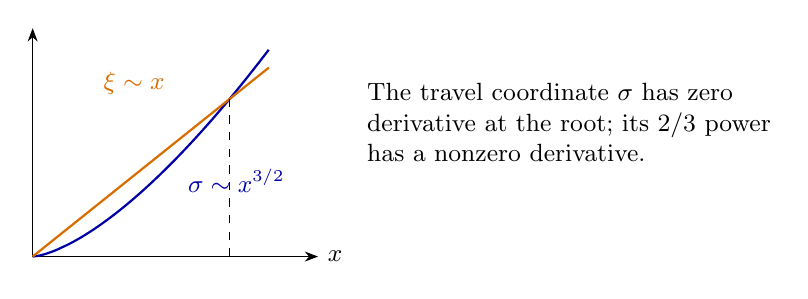
\begin{tikzpicture}[x=2.5cm,y=2.0cm,font=\small,>=Stealth]
\draw[->] (0,0)--(1.45,0) node[right] {$x$};
\draw[->] (0,0)--(0,1.45);
\draw[thick,blue!65!black] plot[domain=0:1.2,samples=50] (\x,{pow(\x,1.5)});
\draw[thick,orange!85!black] (0,0)--(1.2,1.2);
\node[blue!65!black,anchor=west] at (.74,.48) {$\sigma\sim x^{3/2}$};
\node[orange!85!black,anchor=east] at (.72,1.1) {$\xi\sim x$};
\draw[dashed] (1,0)--(1,1);
\node[align=left,anchor=west] at (1.65,.85)
 {The travel coordinate $\sigma$ has zero\\derivative at the root;
  its $2/3$ power\\has a nonzero derivative.};
\end{tikzpicture}
\caption{Regularization at a turning circle; $x$ is the distance to
the root. The graph shows the leading powers with unit coefficients.
The positive coefficient of $x$ in $\xi$ is controlled uniformly at
all turning circles.}
\label{fig:root-regularization}
\end{figure}

\paragraph{The canonical form.}
Let $i\in\{L,R\}$, let $\Psi_i=(\xi_i,\varphi)$ be the coordinate map
on the corresponding half of the component, and put
\[
 \alpha_i=\frac{\delta\circ\Psi_i^{-1}}{\sqrt{\xi_i}}
 =\frac{a\,|\det D\Psi_i|}{U_\theta V_\theta}\circ\Psi_i^{-1},
 \qquad h_i=\alpha_i^{-1/2} .
\]
The second expression shows that $\alpha_i$ is smooth and positive up
to the root. In the coordinates $\Psi_i$ the principal density of
$\widehat L$ is $\alpha_i\,\diag(1,-\xi_i)$, and conjugation by
$h_i$ removes its first-order terms: for
$u=(h_iW_i)\circ\Psi_i$, the equation $\widehat Lu=f$ becomes
\begin{equation}\label{eq:fixed-strip-airy-equation}
 \begin{split}
 \bigl(\partial_{\xi_i}^2-\xi_i\,\partial_\varphi^2+V_i\bigr)W_i&=F_i,\\
 V_i&=-\alpha_i^{-1/2}\,
       \bigl(\partial_{\xi_i}^2-\xi_i\,\partial_\varphi^2\bigr)\,
       \alpha_i^{1/2},\\
 F_i&=h_i\,\Bigl(\frac{f}{|\det D\Psi_i|}\circ\Psi_i^{-1}\Bigr).
 \end{split}
\end{equation}
The principal part is the Tricomi operator
$\partial_\xi^2-\xi\,\partial_\varphi^2$, the same for all states;
only the potential $V_i$ depends on the state. The transformation of
the source preserves the pairing:
$\int uf\,dr\,d\theta=\int W_iF_i\,d\xi_i\,d\varphi$. We call
$W_i$ the \emph{canonical unknown}, $h_i$ the \emph{height factor}
and $F_i$ the \emph{canonical source}.

\paragraph{Transmission in the middle.}
The two halves meet at $\sigma=T/2$, where
$\xi_L=\xi_R=\xi_c:=(3T/4)^{2/3}$. There $\alpha_L=\alpha_R$ and
$\partial_\sigma\log\alpha_R-\partial_\sigma\log\alpha_L=\xi_c^{-3/2}$.
Continuity of $u$ and of its derivative therefore reads
\begin{equation}\label{eq:fixed-strip-cut}
 \binom{W_R}{\partial_{\xi_R}W_R}
 =\begin{pmatrix}1&0\\-1/(2\xi_c)&-1\end{pmatrix}
       \binom{W_L}{\partial_{\xi_L}W_L}
 \qquad\text{at }\xi_L=\xi_R=\xi_c .
\end{equation}
This matrix does not depend on the state.

\paragraph{Boundary data at a root.}
At a root, where the boundary chart is $h_{\rm bd}$ ($=h_L$ or $h_R$),
the value of $u$ and its inward normal flux $p_{\rm in}$ are
\begin{equation}\label{eq:fixed-strip-root-pair}
 u=(h_iW_i)(0,h_{\rm bd}),\qquad
 p_{\rm in}=\frac{h_{\rm bd}'}{h_i(0,h_{\rm bd})}\,
       \bigl(\partial_{\xi_i}W_i+(\partial_{\xi_i}\log h_i)\,W_i\bigr)
                                             (0,h_{\rm bd}) .
\end{equation}
No tangential derivative of $W_i$ appears, because
$a\varphi_r+\widehat b\varphi_\theta=0$ at the root. The identity is
exact; it retains the zero mode and the full Green pairing, not only
the principal part.

\paragraph{Bounds.}
At the reference state all these objects are explicit functions of
$r$; their bounds by coefficient powers are proved in
Lemma~\ref{lem:reference-regularized-charts}. For a general state
they are estimated in Lemma~\ref{lem:current-geometric-jets}.

\subsection{Coordinates on a positive component}
\label{subsec:positive-crossing}

\paragraph{The reference coordinate.}
On a positive component, continue the root coordinates of the two
adjacent roots across them and put $y_i=-\xi_i$, which is positive on
the positive side; here $i=L$ at the left end of the positive
component and $i=R$ at its right end. Choose a coordinate
$y\in[0,1]$, a function of $r$, equal to $y_L$ near the left end and
to $1-y_R$ near the right end, by prescribing its derivative: the
given derivatives on disjoint collars of the two ends and a positive
constant in between, interpolated with cutoffs. Similarly
interpolate the logarithms of the two height factors $h_i$, taking the
height factor equal to one in the middle. The explicit formulas are
\eqref{eq:geometry-positive-coordinate} and
\eqref{eq:geometry-positive-height}; that all these reference
quantities have coefficient bounds is
Lemma~\ref{lem:positive-reference-charts}.

\paragraph{The coordinate of a general state.}
For a general state the coordinates and height factors of the
adjacent negative components differ from the reference ones. Extend
these \emph{differences} into the positive component: the jets of the
coordinates up to order four and the jets of the logarithms of the
height factors up to order three, by Taylor polynomials multiplied
with cutoffs. The cutoffs are chosen so that the reference
coordinate is unchanged on a fixed compact interval $J_*$ of radii
which contains the support of $g_*$ in the normalization $\ell_*$ and
the support of the metric control $\chi_*$. Since the differential is
close to the reference one, the resulting map $\Psi_{\bx}$ is a
diffeomorphism onto $[0,1]\times\T$: it is proper, locally invertible,
and of degree one on the boundary. It obeys the estimates of
Proposition~\ref{prop:uniform-physical-geometry}.

\paragraph{The canonical operator.}
Let $h_{\bx}$ be the height factor in the original variables,
$\Psi_{\bx}$ the coordinate map and $J_{\bx}$ its Jacobian
determinant. For the equation $-\widehat Lu=F_{\rm ph}$ on a positive
component, the canonical operator and source are
\begin{equation}\label{eq:pp-fixed-canonical-source}
 P_{\bx}U
 =-\Bigl(\frac{h_{\bx}}{|J_{\bx}|}\,
       \widehat L\bigl[h_{\bx}\,(U\circ\Psi_{\bx})\bigr]\Bigr)
             \circ\Psi_{\bx}^{-1},\qquad
 F=\Bigl(\frac{h_{\bx}F_{\rm ph}}{|J_{\bx}|}\Bigr)
             \circ\Psi_{\bx}^{-1} .
\end{equation}
These formulas again preserve the pairing. At the reference state
\[
 P_*=-\partial_y(a\,\partial_y)-c\,\partial_\varphi^2+V,
 \qquad a=h_*^2\,w_*\,y_r,\quad c=\frac{h_*^2\,w_*'}{r\,y_r},
\]
where in this formula $a$ and $c$ denote the coefficients of $P_*$.
Near a root $a=1$ and $c=y_i$ exactly: $P_*$ is the continuation
$-\partial_{y_i}^2-y_i\,\partial_\varphi^2$ of the Tricomi operator.
On the whole component, with
\[
 \bd=y\,(1-y),
\]
we have
\begin{equation}\label{eq:positive-coefficients}
 a\ge\mathcal E_m^{-C},\qquad c\ge\mathcal E_m^{-C}\,\bd ,
\end{equation}
and all derivatives of the coefficients of fixed order are bounded by
coefficient powers
(Lemma~\ref{lem:positive-reference-charts}); away from the roots
this comes from the lower bounds for $w_*'/w_*$ on the positive parts
of the models and on the joins.

\paragraph{The difference vanishes to third order at the roots.}
Since the jets specified above match the principal densities of
$P_{\bx}$ and $P_*$ to second order at both roots,
\begin{equation}\label{eq:readable-positive-difference}
 P_{\bx}-P_*=-\partial_a\bigl(\bd^{\,3}\,e_{\bx}^{ab}\,\partial_b\bigr)
                           +\delta V_{\bx} ,
\end{equation}
with smooth coefficients $e^{ab}_{\bx}$, where $a,b$ are indices
running over $y,\varphi$, and a potential $\delta V_{\bx}$ on which no
boundary condition is imposed. Division by $\bd^3$ has a fixed cost:
if $F$, $F'$ and $F''$ vanish at $0$, then
\[
 \frac{F(y)}{y^3}=\frac12\int_0^1(1-t)^2\,F'''(ty)\,dt ,
\]
each further derivative differentiates the integrand, and the factor
$t^{-1/2}$ produced by rescaling in $L^2$ is integrable. This is the
content of part~(iii) of
Proposition~\ref{prop:uniform-physical-geometry}
(Lemma~\ref{lem:current-geometric-jets}, Step~4). The
cubic vanishing is what will allow a second-order perturbation to be
controlled without boundary conditions
(Section~\ref{subsec:cubic-estimate}).

\subsection{Proof of the uniform geometric calculus}
\label{subsec:geometry-proofs}

We prove Proposition~\ref{prop:uniform-physical-geometry}. The bounds
at the reference state come first; they involve functions of $r$ only
(Lemmas~\ref{lem:reference-regularized-charts}--\ref{lem:geometric-weight-conversion}).
The bounds for a general state follow from them and from the lemmas
on flows
(Lemmas~\ref{lem:uniform-characteristic-flow-constants}
and~\ref{lem:current-geometric-jets}). Positivity of a function is
never used as a bound for its reciprocal: every reciprocal that
occurs is bounded explicitly.

\begin{lemma}[Root charts of the reference profile]
\label{lem:reference-regularized-charts}
\label{lem:reference-height-source-factors}
On each half of the negative component of cell $n$, the root
coordinate of the reference profile is the function of $r$
\begin{equation}\label{eq:geometry-regular-root-coordinate}
 \xi=x\,\Bigl[\tfrac32\int_0^1\sqrt t\;c_i(xt)\,dt\Bigr]^{2/3},
\end{equation}
where $x$ is the distance from the root of that half, and
\begin{equation}\label{eq:geometry-root-inverse}
 \mathcal E_n^{-C}\le|\xi_r|\le\mathcal E_n^{C},\qquad
 \|\xi\|_{C^s}+\|r(\xi)\|_{C^s}\le C_s\,\mathcal E_n^{C_s}.
\end{equation}
Moreover
\begin{equation}\label{eq:geometry-root-density}
 \alpha_i=w_*\,|\xi_r|,\qquad h_i=\alpha_i^{-1/2},
\end{equation}
and the functions $\alpha_i^{\pm1}$, $h_i^{\pm1}$, $|\xi_r|^{\pm1}$,
the potential $V_i=-\alpha_i^{-1/2}\partial_\xi^2\alpha_i^{1/2}$, the
source factors $h_i/|\xi_r|$ and $|\xi_r|/h_i$, and
$\partial_\xi\log h_i$ have derivatives of order $s$ bounded by
$C_s\mathcal E_n^{C_s}$. These bounds persist when the half is
rescaled to unit length.
\end{lemma}

\begin{proof}
At the reference state the charts are the identity, so
$\varphi=\theta$ and, on each half, $\xi=(\tfrac32\sigma_i)^{2/3}$,
where $\sigma_i=\int v_0\,dr$ is the travel angle from the root of
that half.

\step{1: near the root}
Since $v_0=\sqrt x\,c_i(x)$, the substitution $x'=xt$ gives
$\sigma_i=x^{3/2}\int_0^1\sqrt t\,c_i(xt)\,dt$, which is
\eqref{eq:geometry-regular-root-coordinate}. The bracket is smooth
and positive, and equals $c_i(0)$ at $x=0$; so
$|\xi_r|=c_i(0)^{2/3}$ at the root. On the collar
$|x|<8\delta_n^{\rm root}$ the bracket lies between
$\tfrac12c_i(0)$ and $2c_i(0)$, and by
\eqref{eq:geometry-normalized-root-jets} its logarithmic derivative
times $|x|$ is at most $C\epsilon_{\rm root}A_n^{15}$. Hence
$|\xi_r|$ is comparable to $c_i(0)^{2/3}$ on the collar, and the
derivatives of $\xi$ have coefficient bounds there.

\step{2: away from the collars}
Differentiating $\xi^{3/2}=\tfrac32\sigma_i$ gives
$|\xi_r|=v_0/\sqrt\xi$, so we need upper and lower bounds for $v_0$
and $\xi$. In the model coordinate the collar of the left root ends
at a distance comparable to $A_n^{19}$ from $X_L$, and that of the
right root at a distance comparable to $A_n^{15}$ from $X_R$, because
$r_X$ is comparable to $\mathfrak r_nA_n$ and $\mathfrak r_nA_n^5$
there. The function $\rho$ has one maximum on the component and
vanishes only at its two ends, where $|\rho_X|$ is comparable to
$A_n$ and $A_n^9$. Hence $\rho\ge cA_n^{24}$ outside the collars, and
\[
 c\,\mathfrak r_n^{-1}A_n^{11}\le v_0=\frac{\sqrt\rho}{r_X}
 \le C\,\mathfrak r_n^{-1}A_n^{-9/2}.
\]
By Step~1, $\xi\ge cA_n^{20}$ at the end of its collar, hence beyond
it, and $\xi\le\xi_c=(3T_n/4)^{2/3}\asymp A_n^{1/3}$. So $|\xi_r|$ is
bounded above and below by powers of $A_n$. The higher derivatives
follow by differentiating $\xi_r=\pm v_0\,\xi^{-1/2}$, using the lower
bounds for $r_X$, $\rho$ and $\xi$ on this region.

\step{3: the inverse}
From $r(\xi(r))=r$ we get $r_\xi=1/\xi_r$, and every higher
derivative of $r(\xi)$ is a polynomial in lower ones and in
derivatives of $\xi$, divided by $\xi_r$. This proves
\eqref{eq:geometry-root-inverse}. The length $\xi_c$ of a half and
its reciprocal are powers of $A_n$, so rescaling to unit length costs
a fixed power of $A_n$ for each derivative.

\step{4: the factors}
For the reference operator $a=w_*$, $\widehat b=0$,
$\delta=w_*v_0$, $U_\theta=V_\theta=1$ and
$|\det D\Psi_i|=|\xi_r|$. Hence
$\alpha_i=\delta/\sqrt\xi=w_*|\xi_r|$, which is
\eqref{eq:geometry-root-density}. By
\eqref{eq:geometry-profile-jets} and \eqref{eq:geometry-root-inverse}
the functions $\alpha_i^{\pm1}$ have coefficient bounds, and the
remaining quantities are obtained from $\alpha_i$ and $\xi_r$ by
products, powers and differentiation in $\xi$. All of them are
functions of $r$, so no angular frequency is involved.
\end{proof}

\begin{lemma}[The reference coordinate on a positive component]
\label{lem:positive-reference-charts}
\label{lem:positive-reference-coefficient-bounds}
Let $(r_1,r_2)$ be a positive component with index $n$, let
$y_L,y_R$ be the continued root coordinates at its two ends, and let
$\eta_L,\eta_R$ be cutoffs with disjoint supports in the collars of
the two ends, equal to one on smaller collars. Define
\begin{equation}\label{eq:geometry-positive-coordinate}
 \begin{split}
 y_r&=\eta_L\,(y_L)_r-\eta_R\,(y_R)_r+\mu_0\,(1-\eta_L-\eta_R),
 \qquad y(r)=\int_{r_1}^ry_r\,dr,\\
 \mu_0&=\frac{1-\int\eta_L\,(y_L)_r\,dr+\int\eta_R\,(y_R)_r\,dr}
            {\int(1-\eta_L-\eta_R)\,dr},
 \end{split}
\end{equation}
and
\begin{equation}\label{eq:geometry-positive-height}
 \log h_*=\eta_L\log h_L+\eta_R\log h_R,
 \qquad h_i=\bigl(w_*\,|(y_i)_r|\bigr)^{-1/2}.
\end{equation}
Then $y$ is a diffeomorphism of $[r_1,r_2]$ onto $[0,1]$ with
$y=y_L$ near $r_1$ and $y=1-y_R$ near $r_2$, and $y_r^{\pm1}$,
$h_*^{\pm1}$, the inverse function $r(y)$ and the source factors
$h_*/y_r$, $y_r/h_*$ have derivatives of order $s$ bounded by
$C_s\mathcal E_n^{C_s}$. The coefficients of the reference operator
$P_*=-\partial_y(a\,\partial_y)-c\,\partial_\varphi^2+V$ are
\begin{equation}\label{eq:geometry-positive-coefficients}
 a=h_*^2\,w_*\,y_r,\qquad
 c=\frac{h_*^2\,w_*'}{r\,y_r},\qquad
 V=-\frac{h_*}{y_r}\,\bigl(w_*\,h_{*,r}\bigr)_r .
\end{equation}
Near the ends $a=1$ and $c=y_i$; on the whole component
\eqref{eq:positive-coefficients} holds, and the derivatives of order
$s$ of $a$, $c$, $V$ and $a^{-1}$ are bounded by
$C_s\mathcal E_n^{C_s}$. On the component which contains the interval
$J_*$, the collars can be chosen disjoint from $J_*$.
\end{lemma}

\begin{proof}
\step{1: the collars}
The continued coordinates $y_i=-\xi_i$ have positive inward
derivatives with the bounds of
Lemma~\ref{lem:reference-regularized-charts}, since
\eqref{eq:geometry-normalized-root-jets} holds on both sides of the
root. The increment of $y_i$ over its collar is at most
$8\delta^{\rm root}\sup|\xi_r|=O(A_n^{18})$. So, after
$\epsilon_{\rm root}$ is decreased if necessary and finitely many
central collars are chosen by hand, the two collars together account
for less than $\tfrac14$ of the total increment $1$. The interval
$J_*$ has positive distance from the roots.

\step{2: the coordinate}
Note that $(y_R)_r<0$, since $y_R$ increases inwards from the right
end. The numerator of $\mu_0$ lies between $\tfrac34$ and $1$, and its
denominator is comparable to $r_2-r_1$; so $\mu_0$ and $\mu_0^{-1}$
are coefficient powers. The function $y_r$ is a convex combination of
positive functions with coefficient bounds above and below, and its
integral over the component is $1$ by the choice of $\mu_0$. Hence
$y=y_L$ near $r_1$ and $y=1-y_R$ near $r_2$, and the inverse function
is estimated as in Step~3 of the preceding proof.

\step{3: the height factor}
The logarithms $\log h_i$ are bounded by $C(n^{5/2}+n^2)$ by
\eqref{eq:geometry-profile-jets}, and their derivatives of positive
order have coefficient bounds. Differentiating
\eqref{eq:geometry-positive-height} and exponentiating gives the
bounds for $h_*^{\pm1}$.

\step{4: the coefficients}
The formulas \eqref{eq:geometry-positive-coefficients} follow by
inserting $u=h_*\,U(y(r))\cos(j\theta)$ into
$-(h_*/y_r)\,\mathscr L_{w_*}u$; the terms with $U_y$ which do not
belong to $(aU_y)_y$ cancel. In a collar
$h_*=(w_*\,|(y_i)_r|)^{-1/2}$ gives $a=1$. Differentiating
\eqref{eq:geometry-regular-root-coordinate} gives
$\xi\,\xi_r^2=x\,c_i(x)^2=-w_*'/(rw_*)$ on both sides of the root, so
$w_*'/(rw_*)=y_i\,(y_i)_r^2$ and $c=y_i$. The upper bounds and the
lower bound for $a$ follow from Steps~2 and~3.

\step{5: the lower bound for $c$}
It suffices to show
\begin{equation}\label{eq:geometry-wprime-distance}
 w_*'(r)\ge\mathcal E_n^{-C}\,\min(r-r_1,\,r_2-r),
\end{equation}
because $y(1-y)\le\mathcal E_n^{C}\min(r-r_1,r_2-r)$ by the bounds
for $y_r$. On a short positive cap
$-\rho\ge cA_n\min(|X-X_L|,1)$, and on a long positive cap
$-\rho\ge cA_n^9\min(|X-X_R|,1)$; since
$w_*'=-\lambda_n\rho\,r/r_X$, the bounds of Lemma~\ref{lem:cell} give
\eqref{eq:geometry-wprime-distance} on the caps. On a join
$w_*'/w_*\ge2/r$ by \eqref{eq:join-slope}, and on the connectors of
Lemma~\ref{lem:connector} $w_*'/w_*\ge3/(4r)$; with the lower bound
for $w_*$ this gives \eqref{eq:geometry-wprime-distance} there, since
the distance to the ends is bounded.
\end{proof}

\begin{lemma}[Conversion of weights and derivatives]
\label{lem:geometric-weight-conversion}
On cell $n$ and its neighbours, the continuous weights $H$, $E_0$,
$M$ and the discrete weights $H_n$, $\mathcal E_n$, $M_n$ differ by
factors bounded by $\mathcal E_n^{C}$. Changes between the variables
$r$, $\varrho$, the root coordinates and the coordinates $y$ transfer
derivatives of total order $s$ to derivatives of total order at most
$s$, with coefficients bounded by $E_0^{C_s}$; so do the source
factors and cutoffs. A restriction to a circle costs one radial
derivative.
\end{lemma}

\begin{proof}
By \eqref{eq:geometry-endpoint-distance},
$x_\partial=n+O(1)$ on cell $n$, so
\[
 \log\frac H{H_n}=O(n^2),\qquad
 \log\frac{E_0}{\mathcal E_n}=O\bigl(n^{3/2}\log(e+n)\bigr),\qquad
 \log\frac M{M_n}=O\bigl(n^{3/2}\log^2(e+n)\bigr),
\]
and the same bounds hold for the ratios of the weights of
neighbouring cells; all of them are $O(\log\mathcal E_n)$. In the
variable $\varrho$,
\[
 |\Dr\log M|\le C\,(1+x_\partial)^{-1/2}\log^2(e+x_\partial),
\]
which is bounded together with its derivatives, and the same is true
of $\log H$, $\log E_0$ and $\log\ell$; so the weights are uniformly
comparable on unit intervals of $\varrho$, and $\ell^{\pm1}$ is
bounded by a power of $E_0$. The chain rule expresses derivatives of
total order $s$ in one set of variables through derivatives of order
at most $s$ in another, with coefficients which are polynomials in the
derivatives of the coordinate functions and in reciprocals of their
first derivatives; these are bounded by
Lemmas~\ref{lem:reference-regularized-charts}
and~\ref{lem:positive-reference-charts}. The inequality
$E_0^{C_s}\le C_sM$ is applied to the complete product. The trace
inequality on an interval of unit length costs one derivative, and
the rescaling to unit length costs coefficient powers.
\end{proof}

\begin{lemma}[Flows at a general state]
\label{lem:uniform-characteristic-flow-constants}
On the neighbourhood of
Lemma~\ref{lem:common-geometric-neighborhood}, after $b_0$ is
increased and $\epsilon_0$ decreased, the characteristic speeds
$c_\pm=d\pm v$ of $\bar L$ on a negative component $m$ satisfy, away
from the collars of the roots,
\begin{equation}\label{eq:geometry-flow-low-bound}
 \int\|\partial_\theta c_\pm(r,\cdot)\|_{H^s_\theta}\,dr
 \le C_s\,\mathcal E_m^{C_s}\,H_m^\beta\;\mathfrak g_{s+d_*,m},
\end{equation}
and the right sides of the regularized equation
\eqref{eq:fixed-strip-root-flow} in the collars, and the corrected
speeds $\widehat c_\pm$ of
Proposition~\ref{prop:optical-residual-completion}, satisfy the same
bound. Consequently the angular derivatives of all characteristic
flows and of their inverses lie in $[\tfrac12,2]$, and the constants
of Lemma~\ref{lem:circle-flow} for these flows are uniform in $m$.
\end{lemma}

\begin{proof}
\step{1: the speeds}
By \eqref{eq:completed-characteristics},
\[
 d=\frac{E\,(p-k_\theta)}{rQ},\qquad
 v=\sqrt{-\frac{w'}{rw}}\;\frac{w\sqrt D}{Q},
 \qquad -\frac{w'}{rw}=v_0^2-\frac{f'}r,
\]
where $w=w_*e^f$. At the reference state $d=0$ and $v=v_0$. The
quantities $d$ and $w\sqrt D/Q-1$ are coefficients in the sense of
Step~3 of the proof of Lemma~\ref{prop:full-physical-tame}, and they
vanish at the reference state. Outside the supports of the controls
$f'=0$; on the support of $\chi_n$ the ratio $f'/(rv_0^2)$ is bounded
by $C|\kappa_n|A_n^{-29}$, with derivatives bounded by coefficient
powers times $|\kappa_n|$
(Lemma~\ref{lem:quantitative-optical-controls}). So $v/v_0-1$ is of
the same kind. Only the deformation depends on $\theta$, and the
length of the component is bounded; this proves
\eqref{eq:geometry-flow-low-bound}. In a collar write
$v=\sqrt x\,c_0(x,\theta)$ with
$c_0=c_i(x)\cdot(v/v_0)$; by Lemma~\ref{lem:quantitative-root-collars}
the function $c_0$ and its reciprocal have coefficient bounds, and
$c_0-c_i$ and $d$ are bounded as in
\eqref{eq:geometry-flow-low-bound}. The equation
\eqref{eq:fixed-strip-root-flow} involves $d$ and $c_0$ at the point
$xt^2$ and the bounded factors $x$ and $\zeta$, so its right side has
the same bounds.

\step{2: the Jacobians}
Rescale the radial variable on each part of the component to the unit
interval; this multiplies the speeds by lengths, which are coefficient
powers. By \eqref{eq:geometry-smallness-absorption}, the right side of
\eqref{eq:geometry-flow-low-bound} for $s\le4$ is as small as we wish
on the neighbourhood, uniformly in $m$. Lemma~\ref{lem:circle-flow}
then gives the bounds for the angular derivatives of the flows; the
derivative of an inverse flow is the reciprocal of that of the flow.
The large speed $v_0$ of the reference profile does not enter,
because it does not depend on $\theta$.

\step{3: the corrected flow}
The corrected minus flow is $\widehat\Phi_r=\Phi_r\circ J_r$ with
$J_r=\id+\chi(r)\Delta$, and its speed is
\eqref{eq:readable-optical-velocity}. At the reference state
$\Delta=0$. By the definition of $\Delta$ in the proof of
Proposition~\ref{prop:optical-residual-completion} and
Lemma~\ref{lem:one-high-factor}(iv), $\Delta$ is estimated by the
return residual, hence by the right side of
\eqref{eq:geometry-flow-low-bound}; the cutoff $\chi$ has
coefficient bounds, and on the support of $\chi'$ the speed $v$ is
bounded below by a coefficient power, so the correction is smaller
than $v/2$. It vanishes near both roots, so the functions $c_0$ are
unchanged. Thus Steps~1 and~2 apply to the corrected flows.
\end{proof}

\begin{lemma}[Coordinates and factors at a general state]
\label{lem:current-geometric-jets}
On the same neighbourhood, with a fixed $d_*$, every coordinate,
inverse coordinate, Jacobian, height factor, source factor, potential
and divided coefficient of
Sections~\ref{subsec:return-correction}--\ref{subsec:positive-crossing}
satisfies \eqref{eq:geometry-current-jet-bound}, and its derivatives
with respect to the state satisfy the corresponding estimates of the
shape \eqref{eq:tame-derivative-shape}.
\end{lemma}

\begin{proof}
We follow the order in which the objects were constructed. No norm of
high order is assumed small.

\step{1: flows and root coordinates}
Away from the collars, the last statement of
Lemma~\ref{lem:circle-flow} bounds the difference between the flows
of a general state and of the reference state by the difference of
the speeds, that is, by the right side of
\eqref{eq:geometry-flow-low-bound}. In a collar the same lemma
applies to \eqref{eq:fixed-strip-root-flow}, whose right side is
smooth in the independent variables $(x,\zeta,\theta)$; so the
function $G(x,\zeta,\theta)$ of Section~\ref{subsec:root-coordinate},
minus its reference value, satisfies
\eqref{eq:geometry-current-jet-bound} in all three variables.
Lemma~\ref{lem:rewrite-root-composition} then gives the bound for
$\varphi=\Ev\,G$, and for $\chi_0=\Od\,G$ with one additional
derivative; and $\xi_L=x\,(\tfrac32\chi_0)^{2/3}$ is a smooth function
of $\chi_0$, which is bounded below. The charts $h_R$ and the residual
$\mathfrak e$ are obtained from $h_L$ and the return map by
compositions, inversions and parity projections, to which
Lemma~\ref{lem:one-high-factor}(iv) applies. The corrected flows were
treated in Lemma~\ref{lem:uniform-characteristic-flow-constants}.

\step{2: inverse coordinates, height factors and sources}
At low order, Step~1 and \eqref{eq:geometry-root-inverse} give, for
the coordinate maps rescaled to unit size,
\[
 \bigl\|(D\Psi-D\Psi_*)\,(D\Psi_*)^{-1}\bigr\|_{C^0}
 \le C\,\epsilon_0\,H_m^\beta\,\mathcal E_m^{C}<\tfrac14
\]
on the neighbourhood, by \eqref{eq:geometry-smallness-absorption}. So
$D\Psi$ is invertible with bounds comparable to the reference. The
higher derivatives of $\Psi^{-1}$ follow by differentiating
$\Psi^{-1}\circ\Psi=\id$; subtracting the reference identity and
using the product estimate keeps the factor of the difference. For
the density use the identity
\[
 \alpha_i=\frac{a\,|\det D\Psi_i|}{U_\theta V_\theta}\circ\Psi_i^{-1}
\]
of Section~\ref{subsec:root-coordinate}: the Jacobian of the
regularized coordinates does not vanish, and $U_\theta V_\theta$ is
bounded below by
Lemma~\ref{lem:uniform-characteristic-flow-constants}. Powers,
derivatives and the formulas \eqref{eq:fixed-strip-airy-equation}
then give the height factor, the potential and the source factor. The
reciprocal of the Jacobian of the unregularized coordinates
$(\sigma,\varphi)$, which vanishes at the roots, is never used.

\step{3: positive components}
The coordinate and the height factor of a general state on a positive
component are the reference ones plus Taylor polynomials, of degree
four and three, of the differences at the two ends, multiplied by
fixed cutoffs. Restriction to the boundary, the polynomials and the
cutoffs preserve the bounds of Steps~1 and~2. The differential stays
close to the reference one as in Step~2, so the Jacobian is positive,
and the inverse coordinate and the source factor are estimated in the
same way.

\step{4: division by $\bd^3$}
The differences $F$ of the principal densities vanish with their
first two inward derivatives at both ends. Near the left end
\[
 \frac{F(y)}{y^3}=\frac12\int_0^1(1-t)^2\,F'''(ty)\,dt,
\]
which costs three derivatives and keeps the factor $H_m^\beta$; near
the right end divide by $(1-y)^3$ in the same way; in the middle
$\bd^{-1}$ has coefficient bounds. This gives the bound for
$e^{ab}_{\bx}=F^{ab}/\bd^3$.

\step{5: the loss and the parameters}
The characteristic speeds involve two derivatives of the height; the
divided difference at a root one more; the boundary polynomials four;
the principal density one derivative of the coordinates; the potential
two more; the division three; and the Sobolev embedding and the
traces a fixed number. Their total is $d_*$, which does not depend on
$s$. Derivatives with respect to the state are estimated by
differentiating the same finite formulas and the equations of the
flows: every variation of a flow solves a linear equation with the
same integrating factor, which is bounded by Step~2 of the preceding
proof. The height enters through $Z=qu$, whose first derivative is
$\dot q\,u+q\,\dot u$, whose second derivative is $q_1u_2+q_2u_1$, and
whose higher derivatives vanish. Hence the seminorms
\eqref{def:joint-displacement-seminorms}, which contain the unscaled
$u$, control all derivatives, also at $q=0$. Finally
Lemma~\ref{lem:geometric-weight-conversion} absorbs each complete
product of reference functions into one power of $M$.
\end{proof}

\begin{proof}[Proof of Proposition~\ref{prop:uniform-physical-geometry}]
Part~(i) is Lemmas~\ref{lem:reference-regularized-charts}
and~\ref{lem:positive-reference-charts}, with
Lemmas~\ref{lem:quantitative-root-collars}
and~\ref{lem:quantitative-optical-controls} for the collars, the
controls and the cutoffs. Parts~(ii) and~(iii) are
Lemmas~\ref{lem:uniform-characteristic-flow-constants}
and~\ref{lem:current-geometric-jets}; the comparability of the
differentials was shown in Step~2 of the last proof. All collars and
cutoffs were chosen before any order of differentiation; only the
constants depend on the order.
\end{proof}

\subsection{The fixed transmission domain}
\label{subsec:transmission-domain}

We have represented a height on the annulus by canonical unknowns on a
collection of cylinders: two half-cylinders
$[0,\xi_c]\times\T$ for each negative component and one cylinder
$[0,1]\times\T$ for each positive component. The cylinders do not
depend on the state. Neither do the conditions that link them:
\begin{itemize}
\item at the middle of a negative component, the condition
 \eqref{eq:fixed-strip-cut};
\item at a root, equality of the canonical values and of the inward
 derivatives with opposite signs. Indeed, the coordinates and the
 height factors of the two adjacent components have the same value
 and the same first derivative at the root, so
 \eqref{eq:fixed-strip-root-pair} takes this form.
\end{itemize}
We call the set of canonical unknowns satisfying these conditions the
\emph{transmission domain}. A smooth element of it which solves the
equation corresponds to a function which is smooth in the original
variables across the roots: equality of the values gives equality of
all tangential derivatives; equality of the fluxes gives equality of
the first normal derivative; and the equation can be solved for
$a\,u_{rr}$, because $a>0$, so that repeated differentiation matches
all higher normal derivatives.

This is the result of the section: all the operators
$\widehat L_{\bx}$ act, in canonical form, on one domain. It is what
makes it possible to regard them as perturbations of the reference
operator in the next section.

\section{Inverting the corrected linearization near the reference}
\label{sec:stable-inverse}
\label{sec:grn-fixed-phase-green}

The goal of this section is
Proposition~\ref{prop:rewrite-volume-inverse}: for every state $\bx$
in the neighbourhood of
Proposition~\ref{prop:uniform-physical-geometry}, the operator
$\widehat L_{\bx}$, bordered by the derivative of the equation with
respect to the metric parameter $\nu$, has an inverse which satisfies
tame estimates.

The argument has to respect one constraint. The reference inverse
loses coefficient weight, and a tame estimate with a loss is not a
bounded inverse on a single Banach space; it cannot by itself justify
a Neumann series. We therefore proceed in three steps.
\begin{enumerate}[label=\textup{\arabic*.}]
\item We put the problem in canonical form and identify a single
 Hilbert space of sources on which the \emph{relative} operator
 $\mathscr R_{\bx}=(\mathbb P_{\bx}-\mathbb P_*)\,\mathbb G_*$ is
 bounded, with small norm. The loss of the reference inverse is
 compensated by the factor $H^\beta$ carried by every difference of
 coefficients
 (Sections~\ref{subsec:canonical-problem}--\ref{subsec:relative}).
\item A Neumann series on that one space gives the solution.
\item All higher regularity of this same solution is then recovered
 from the equation: angular derivatives by commutators, radial
 derivatives by solving the equation for its highest radial
 derivative (Section~\ref{subsec:higher}).
\end{enumerate}
In this order of argument, one neighbourhood of the reference state
serves for all orders of differentiation.

\subsection{The linear problem in canonical form}
\label{subsec:canonical-problem}

\paragraph{Transformations.}
Use the cylinders of Section~\ref{sec:fixed-geometry}. Let
$\Psi_{\bx}$ denote the coordinate map on each piece, $J_{\bx}$ its
Jacobian determinant and $h_{\bx}$ the height factor in the original
variables. Define
\[
 \mathscr C_{\bx}u=\frac{u}{h_{\bx}}\circ\Psi_{\bx}^{-1},
 \qquad
 \mathscr S_{\bx}f=\frac{h_{\bx}f}{|J_{\bx}|}\circ\Psi_{\bx}^{-1},
 \qquad
 \mathbb L_{\bx}=
 \mathscr S_{\bx}\,\widehat L_{\bx}\,\mathscr C_{\bx}^{-1} .
\]
Thus $\mathscr C_{\bx}$ maps a height to its canonical unknown,
$\mathscr S_{\bx}$ maps a source to its canonical source, and
$\mathbb L_{\bx}$ is the operator in canonical form; on a positive
cylinder $\mathbb L_{\bx}=-P_{\bx}$. The pairing with $dr\,d\theta$ is
preserved. A \emph{piece} is one of the cylinders: a half of a
negative component, or a positive component. A function on the
collection of all pieces is written $F=(F_m)$.

\paragraph{Source norms.}
For real $t$ and integers $s\ge0$ let $\mathbb V_{t,s}$ be the space
of $F=(F_m)$ with
\begin{equation}\label{eq:vol-source-spaces}
 \|F\|_{t,s}^2
 =\sum_m M_m^{2t}\,H_m^{-2\beta}\,
                  \|F_m\|_{L^2_{\rm rad}H^s_\varphi}^2<\infty ,
\end{equation}
where $m$ runs over all pieces, the norm is $L^2$ in the radial
variable of the cylinder with $s$ angular derivatives, and $M_m,H_m$
are the weights of the cell containing the piece. No matching
condition and no integral condition is imposed on sources. The index
$t$ counts powers of the weight $M$, the index $s$ angular
derivatives.

\paragraph{Scalars and the augmented operator.}
The linear problem involves three scalars besides the canonical
unknown $W$.
\begin{itemize}
\item \emph{The endpoint constant $a_L$.} A height is represented as
 \[
  \eta=\mathscr C_{\bx}^{-1}W+a_L\chi_L,\qquad \ell_*^cW=0 ,
 \]
 so that $\eta$ tends to $a_L$ at the left endpoint and to $0$ at the
 right one. The coordinates agree with the reference ones on the
 interval $J_*$ of Section~\ref{subsec:positive-crossing}, which
 contains the support of $g_*$; hence the normalization
 $\ell_*\eta=0$ takes a form $\ell_*^cW=0$ which does not depend on
 the state.
\item \emph{The metric increment $\mu$.} It multiplies the column
 \[
  k_{\bx}=D_\nu\mathcal F_q(w,u),\qquad
  k_{\bx}^c=\mathscr S_{\bx}k_{\bx},
 \]
 where $D_\nu$ is the derivative of the residual with respect to
 $\nu$ for fixed $u$ and $q$; it acts on the metric and on the
 radial height $h$. At the reference state $k_*=g_*e_2$, the border
 column of Proposition~\ref{prop:rad-fixed-theorem}. This scalar
 removes the obstruction in the second mode.
\item \emph{An auxiliary scalar $\lambda$.} Choose a function $\psi$
 of $r$, compactly supported in $J_*$, with $\Qint\psi=1$, and put
 $c_*=\mathscr S_*\psi=\mathscr S_{\bx}\psi$. The scalar $\lambda$
 multiplies $c_*$ and removes the integral obstruction, so that
 arbitrary sources can be treated. For compatible sources it will
 turn out to be zero.
\end{itemize}
With $s_{\bx}=\mathscr S_{\bx}\widehat L_{\bx}\chi_L$, the
\emph{augmented operator} is
\begin{equation}\label{eq:vol-abstract-complete-operator}
 \mathbb P_{\bx}\bW
 =\mathbb L_{\bx}W+a_L\,s_{\bx}+\mu\,k_{\bx}^c+\lambda\,c_*,
 \qquad \bW=(W,a_L,\mu,\lambda) .
\end{equation}
The norm of an output $\bW$ is the norm \eqref{eq:vol-source-spaces}
of $W$ plus the absolute values of the three scalars, which are
assigned to the finite middle part; we write
$\|\bW\|^{\rm vol}_{t,s}$.

\paragraph{The reference inverse in this form.}
At the reference state let $\mathfrak g_*=\mathscr C_*1$ and
$\Qint_*F=\langle\mathfrak g_*,F\rangle$; this functional is
continuous by the coefficient bounds, it is the integral $\Qint$ in
canonical form, and $\Qint_*c_*=1$. Given $F$, put
$\lambda=\Qint_*F$ and apply the inverse of
Proposition~\ref{prop:rad-fixed-theorem} to the compatible source
$F-\lambda c_*$. This defines a two-sided inverse $\mathbb G_*$ of
$\mathbb P_*$. In the zero mode it is explicit: with
$f_*=\mathscr S_*^{-1}F$,
\[
 p_0(r)=\int_{r_-}^r\bigl(\av{f_*}-\lambda\psi\bigr)(t)\,dt,
 \qquad
 u_0(r)=-\int_r^{r_+}\frac{p_0(t)}{w_*(t)}\,dt ,
\]
as in \eqref{eq:rad-eq-rm49}; near either endpoint $p_0$ is the
primitive starting at that endpoint, division by $w_*$ costs a
coefficient power and not an endpoint exponent, and subtracting the
left endpoint value times $\chi_L$ gives the field and the scalar
$a_L$.

\subsection{Two endpoint exponents give decay off the diagonal}
\label{subsec:two-exponents}

By Proposition~\ref{prop:rad-fixed-theorem}(iv),(v) the reference
inverse is bounded with the endpoint weight $H^{-\gamma}$ for every
$\gamma$ in a compact subinterval of $(0,1)$. Fix
\[
 0<\epsilon<\min(\beta,1-\beta).
\]
The inverses at the exponents $\beta-\epsilon$ and $\beta+\epsilon$
coincide on smooth compactly supported sources: their difference is a
homogeneous solution in the graph domain, hence zero by
Lemma~\ref{lem:rad-green-completion}. So both estimates apply to the
same operator $\mathbb G_*$. Using each of them on one side of the
diagonal converts the two bounds into decay in the distance between
source and output (Figure~\ref{fig:two-weights}).

\begin{lemma}[A fixed loss of coefficient weight]
\label{lem:two-weights-closed-domain}
There is a fixed $L_0$ such that for every real $t$ and every
$s\ge0$
\begin{equation}\label{eq:reference-negative-material-extension}
 \|\mathbb G_*F\|^{\rm vol}_{t-L_0,s}\le C_{t,s}\,\|F\|_{t,s} .
\end{equation}
The first radial derivative of $\mathbb G_*F$ satisfies the same
bound with at most one additional angular derivative of the source.
For a fixed integer $b\ge2$,
\begin{equation}\label{eq:fixed-base-graph-domain}
 \mathbb D_*:=\mathbb G_*(\mathbb V_{0,b}),\qquad
 \|\bW\|_{\mathbb D_*}=\|\mathbb P_*\bW\|_{0,b} ,
\end{equation}
is a Hilbert space on which $\mathbb P_*$ is closed. It contains
every smooth $\bW$ in the transmission domain of
Section~\ref{subsec:transmission-domain} which satisfies the
conditions at the endpoints and the normalization, and for which
$\mathbb P_*\bW\in\mathbb V_{0,b}$.
\end{lemma}

\begin{proof}
\step{1: blocks}
Let $\bar S_m=S_m-S_N$ on the tails and $\bar S_m=0$ on the finite
middle. Let $\pi_k$ be the restriction to the piece $k$ and $\iota_m$
the extension by zero of a source on the piece $m$. By
Section~\ref{subsec:interface}, the estimate at the exponent $\gamma$
gives
\[
 \|\pi_k\,\mathbb G_*\,\iota_m\|_{H^s_\varphi\to H^s_\varphi}
 \le C_s\,\mathcal E_k^{C_s}\,\mathcal E_m^{C_s}\,
                        e^{-\gamma(\bar S_k-\bar S_m)} .
\]
There is no loss of angular derivatives, because the reference
inverse acts on each angular mode with bounds uniform in the mode.
Multiply by the weights $H_k^{-\beta}H_m^{\beta}$ of
\eqref{eq:vol-source-spaces}, and use $\gamma=\beta+\epsilon$ when
$\bar S_k\ge\bar S_m$ and $\gamma=\beta-\epsilon$ otherwise. The
resulting block $K_{km}$ satisfies
\begin{equation}\label{eq:global-two-weight-block-bound}
 \|K_{km}\|_{H^s_\varphi\to H^s_\varphi}
 \le C_s\,\mathcal E_k^{C_s}\,\mathcal E_m^{C_s}\,
                    e^{-\epsilon|\bar S_k-\bar S_m|} .
\end{equation}
The estimate for the first radial derivative in
Proposition~\ref{prop:rad-fixed-theorem}(iv) gives the same block
bound with one more angular derivative.

\step{2: summation}
For every $\delta>0$,
$|\log M_k-\log M_m|\le\delta\,|\bar S_k-\bar S_m|+C_\delta$, because
the derivative of $n^{5/2}\log^2(e+n)$ with respect to $2n^3/3$ tends
to zero. With $\mathcal E^{C_s}\le C_sM$ we get, for $L_0\ge2$,
\[
 M_k^{t-L_0}\,\|K_{km}\|\,M_m^{-t}
 \le C_s\,M_k^{2-L_0}\Bigl(\frac{M_k}{M_m}\Bigr)^{t-1}
                         e^{-\epsilon|\bar S_k-\bar S_m|}
 \le C_{t,s}\,e^{-(\epsilon/2)|\bar S_k-\bar S_m|} ,
\]
where $\delta$ was chosen with $|t-1|\,\delta\le\epsilon/2$. This
matrix has bounded row and column sums, since the numbers $S_n$ are
uniformly separated and each index carries a bounded number of
pieces. Schur's test proves
\eqref{eq:reference-negative-material-extension}.

\step{3: the domain}
By definition $\mathbb D_*$ is isometric to $\mathbb V_{0,b}$, hence
complete. If $\bW_i\to\bW$ in the space of outputs and
$\mathbb P_*\bW_i\to F$ in $\mathbb V_{0,b}$, then
$\bW_i=\mathbb G_*\mathbb P_*\bW_i\to\mathbb G_*F$, so
$\bW=\mathbb G_*F$: the operator is closed. Approximating a source by
smooth compactly supported ones, the estimate gives convergence of
the solutions on every piece, the equation passes to the limit in the
sense of distributions, and the bound for the first radial derivative
identifies the traces, so the transmission conditions hold in the
weak sense. Finally, a smooth $\bW$ as in the last statement differs
from $\mathbb G_*\mathbb P_*\bW$ by a normalized homogeneous solution
with the natural behaviour at the endpoints, which vanishes by
Lemma~\ref{lem:rad-green-completion}.
\end{proof}

\begin{figure}[htbp]
\centering
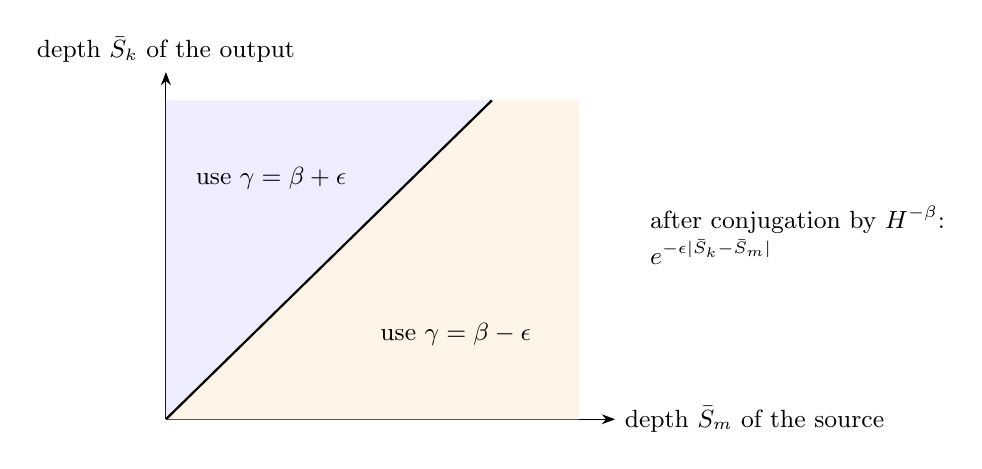
\begin{tikzpicture}[x=.92cm,y=.9cm,font=\small,>=Stealth]
\draw[->] (0,0)--(6.2,0) node[right] {depth $\bar S_m$ of the source};
\draw[->] (0,0)--(0,4.9) node[above] {depth $\bar S_k$ of the output};
\fill[blue!7] (0,0)--(4.5,4.5)--(0,4.5)--cycle;
\fill[orange!9] (0,0)--(5.7,0)--(5.7,4.5)--(4.5,4.5)--cycle;
\draw[thick] (0,0)--(4.5,4.5);
\node at (1.45,3.4) {use $\gamma=\beta+\epsilon$};
\node at (4,1.2) {use $\gamma=\beta-\epsilon$};
\node[align=left,anchor=west] at (6.55,2.6)
 {after conjugation by $H^{-\beta}$:\\[2pt]
  $e^{-\epsilon|\bar S_k-\bar S_m|}$};
\end{tikzpicture}
\caption{The same reference inverse is estimated with two endpoint
weights, each used on one side of the diagonal. Together they give
decay in the distance between the depths of the source and of the
output.}
\label{fig:two-weights}
\end{figure}

\subsection{Positive cylinders: an estimate without boundary conditions}
\label{subsec:cubic-estimate}

On a positive cylinder the perturbation
\eqref{eq:readable-positive-difference} is of second order, the same
order as the operator. It can nevertheless be controlled by the
operator, because its coefficients vanish to third order at the two
ends. The following estimate is the reason for that requirement. In
this subsection $\langle j\rangle=(1+j^2)^{1/2}$.

\begin{lemma}[Weighted graph estimate]\label{lem:cubic}
On $0<y<1$ consider, for an integer $j$,
\[
 P_ju=-(a\,u')'+j^2c\,u+V\,u=F,
 \qquad a\ge\mathcal E_m^{-C},\quad
 c\ge\mathcal E_m^{-C}\,\bd,\quad \bd=y(1-y),
\]
where the derivatives up to order two of $a,c,V$, and $a^{-1}$, are
bounded by $\mathcal E_m^{C_1}$. For every solution
$u\in L^2$ with $F\in L^2$, without any condition at the endpoints,
\begin{equation}\label{eq:vol-arbitrary-boundary-graph-bound}
 \begin{split}
 &\|\bd\,u'\|_2+\langle j\rangle\,\|\bd^{3/2}u\|_2+\|\bd^{2}u''\|_2
   +\langle j\rangle^2\,\|\bd^{3}u\|_2
   +\langle j\rangle\,\|\bd^{5/2}u'\|_2\\
 &\hspace{30mm}\le\mathcal E_m^C\,\bigl(\|F\|_2+\|u\|_2\bigr).
 \end{split}
\end{equation}
\end{lemma}

\begin{proof}
For fixed $j$ a solution in $L^2$ with $F\in L^2$ is in $H^2$ up to
the endpoints, since the equation is a regular ordinary differential
equation; this justifies the integrations by parts below, but the
uniform bounds come from the computation.

\step{1: first order}
Multiply the equation by $\bd^2\bar u$ and integrate. Since $\bd$
vanishes at both ends,
\[
 \int a\,|(\bd u)'|^2+j^2\int c\,\bd^2|u|^2
 =\operatorname{Re}\langle F,\bd^2u\rangle
       +\int a\,|\bd'|^2|u|^2-\int V\,\bd^2|u|^2 .
\]
This bounds $\bd\,u'$ and $j\,\bd^{3/2}u$.

\step{2: second order}
The function $\widetilde u=\bd^2u$ vanishes at both ends and satisfies
\[
 P_j\widetilde u=\bd^2F-2a\,(\bd^2)'u'-(a\,(\bd^2)')'u ,
\]
whose right side is controlled by Step~1. With $\mathsf c=c/a$ the
same is true of
$F_1=-\widetilde u''+j^2\mathsf c\,\widetilde u$. Squaring and
integrating the cross term by parts twice,
\[
 \|\widetilde u''\|_2^2+j^4\|\mathsf c\,\widetilde u\|_2^2
 +2j^2\int\mathsf c\,|\widetilde u'|^2
 =\|F_1\|_2^2+j^2\int\mathsf c''\,|\widetilde u|^2 .
\]
The last integral is controlled by Step~1 because
$\bd^4\le C\bd^3$. Using $\mathsf c\ge\mathcal E_m^{-C}\bd$ and
expressing $\widetilde u'$ and $\widetilde u''$ through $u$ gives
\eqref{eq:vol-arbitrary-boundary-graph-bound}.
\end{proof}

\paragraph{Consequence for the perturbation.}
Every second-order term of \eqref{eq:readable-positive-difference} is
controlled by the left side of
\eqref{eq:vol-arbitrary-boundary-graph-bound}: $\bd^3u_{yy}$ by
$\bd^2u''$, $\bd^3u_{y\varphi}$ by
$\langle j\rangle\bd^{5/2}u'$, and $\bd^3u_{\varphi\varphi}$ by
$\langle j\rangle^2\bd^3u$. When a derivative falls on a coefficient,
the remaining terms are controlled by the first two norms.

The coefficients depend on $\varphi$, and this dependence is handled
by Fourier series. Write $u=\sum_ju_j(y)\,e^{ij\varphi}$ and, for one
of the coefficients, $e=\sum_ke_k(y)\,e^{ik\varphi}$. The $l$th
Fourier coefficient of $\bd^3e\,u_{yy}$ is
$\sum_ke_k\,\bd^3u_{l-k}''$, so
\[
 \bigl\|(\bd^3e\,u_{yy})_l\bigr\|_{L^2_y}\le\sum_k\epsilon_k\,g_{l-k},
 \qquad \epsilon_k=\sup_y|e_k(y)|,\quad
 g_j=\|\bd^2u_j''\|_{L^2_y}
 \le\mathcal E_m^C\bigl(\|F_j\|_2+\|u_j\|_2\bigr),
\]
the last inequality being Lemma~\ref{lem:cubic} for the mode $j$.
Since $\langle l\rangle^s\le2^s(\langle k\rangle^s+\langle l-k\rangle^s)$,
Young's inequality for sequences gives
\begin{equation}\label{eq:sequence-convolution}
 \bigl\|\langle l\rangle^s(\epsilon*g)_l\bigr\|_{\ell^2}
 \le2^s\bigl(\|\epsilon\|_{\ell^1}\,\|\langle j\rangle^sg\|_{\ell^2}
 +\|\langle k\rangle^s\epsilon\|_{\ell^2}\,\|g\|_{\ell^1}\bigr),
\end{equation}
and $\|g\|_{\ell^1}\le C\|\langle j\rangle g\|_{\ell^2}$,
$\|\epsilon\|_{\ell^1}\le C\|\langle k\rangle\epsilon\|_{\ell^2}$.
The weighted norms of $(\epsilon_k)$ are bounded by norms of the
coefficient $e$ with one more derivative in $y$, hence by
\eqref{eq:geometry-current-jet-bound}. The other terms are treated in
the same way, with $g_j$ replaced by the corresponding term on the
left of \eqref{eq:vol-arbitrary-boundary-graph-bound}; for instance
$g_j=\langle j\rangle^2\|\bd^3u_j\|_{L^2_y}$ for the term
$\bd^3e\,u_{\varphi\varphi}$. For the commutator with
$\Lambda=|D_\varphi|$, the $l$th coefficient of $[\Lambda,e]\,v$ is
$\sum_k(|l|-|l-k|)\,e_kv_{l-k}$, and
$\bigl||l|-|l-k|\bigr|\le|k|$; so $\epsilon_k$ is replaced by
$|k|\,\epsilon_k$, which costs one more angular derivative of the
coefficient. Altogether, for $P_*u=F$ on the piece $m$ and $s\ge b$,
\begin{equation}\label{eq:readable-positive-relative-bound}
 \|\delta P_{\bx}u\|_s
 \le C_s\,H_m^\beta\,\mathcal E_m^{C_s}
 \Bigl[\mathfrak g_{b_0,m}\,\bigl(\|F\|_s+\|u\|_s\bigr)
       +\mathfrak g_{s+d_*,m}\,\bigl(\|F\|_b+\|u\|_b\bigr)\Bigr],
\end{equation}
and the same bound holds for $[\Lambda,\delta P_{\bx}]u$. Here
$\delta P_{\bx}=P_{\bx}-P_*$, the norms are those of
$L^2_yH^s_\varphi$, and $\mathfrak g_{s,m}$ is the localized seminorm
of Section~\ref{subsec:neighbourhood}. No artificial boundary
condition was imposed on the reference solution $u$.

\paragraph{An elementary estimate for the first radial derivative.}
On every piece, normalized to unit radial length, the equation at
frequency $j$ has the form $Au''+Bu'+(j^2C+D_0)u=F$, with $A$ bounded
away from zero and all coefficients bounded by coefficient powers.
From the equation and the interpolation inequality
$\|u'\|_2^2\le C\|u\|_2(\|u''\|_2+\|u\|_2)$,
\begin{equation}\label{eq:vol-reference-first-normal-bound}
 \|u'\|_2\le\mathcal E_m^C\bigl(\|F\|_2+\langle j\rangle\|u\|_2\bigr),
 \qquad
 \|u''\|_2\le\mathcal E_m^C\bigl(\|F\|_2+\langle j\rangle^2\|u\|_2\bigr),
\end{equation}
with no assumption on the boundary values: substitute the equation
for $u''$ into the interpolation inequality and absorb the term
$\mathcal E_m^C\|u\|_2\|u'\|_2$ by Young's inequality. Smooth sources
with finitely many frequencies are dense, and for limits of such
sources these estimates identify the weak derivatives; so no
regularity is assumed beforehand.

\subsection{The relative operator}
\label{subsec:relative}

On smooth compactly supported sources define
\[
 \mathscr R_{\bx}=(\mathbb P_{\bx}-\mathbb P_*)\,\mathbb G_* .
\]
If $\mathbb G_*F=(W,a_L,\mu,\lambda)$, then
\begin{equation}\label{eq:vol-normalized-relative-identity}
 \mathscr R_{\bx}F
 =\delta\mathbb L_{\bx}W
      +a_L\,(s_{\bx}-s_*)+\mu\,(k_{\bx}^c-k_*^c),
 \qquad\delta\mathbb L_{\bx}=\mathbb L_{\bx}-\mathbb L_* ;
\end{equation}
the column $c_*$ does not depend on the state. On a negative piece
$\delta\mathbb L_{\bx}$ is the difference of the potentials $V_i$ in
\eqref{eq:fixed-strip-airy-equation}, a multiplication operator. On a
positive piece it is estimated by
\eqref{eq:readable-positive-relative-bound}, the compactly supported
scalar columns being counted as part of the source. In every case the
difference of coefficients on the output piece $k$ carries the factor
$H_k^\beta$ of \eqref{eq:geometry-current-jet-bound}.

\begin{lemma}[The relative operator is small on one space]
\label{lem:relative}
Let $b\ge2$ be as in Lemma~\ref{lem:two-weights-closed-domain}. After
$b_0$ is increased and $\epsilon_0$ decreased,
\begin{equation}\label{eq:rewrite-base-relative}
 \|\mathscr R_{\bx}\|_{\mathbb V_{0,b}\to\mathbb V_{0,b}}
                         \le C\,\mathfrak n_{b_0}<\tfrac12 .
\end{equation}
Moreover, for $t\ge0$ and $s\ge b$, with $\Lambda=|D_\varphi|$,
\begin{equation}\label{eq:compact-volume-relative-bound}
 \|\mathscr R_{\bx}F\|_{t,s}
 +\|[\Lambda,\mathscr R_{\bx}]F\|_{t,s}
 \le C_{t,s}\bigl[\epsilon_0\,\|F\|_{0,s}
             +\mathfrak n_{t+s+d_*}\,\|F\|_{0,b}\bigr] .
\end{equation}
The operator $\mathscr R_{\bx}$ extends by continuity to
$\mathbb V_{0,b}$, and
\begin{equation}\label{eq:current-fixed-domain-factorization}
 \mathbb P_{\bx}=(I+\mathscr R_{\bx})\,\mathbb P_*
                         \qquad\text{on }\mathbb D_* .
\end{equation}
\end{lemma}

Note that \eqref{eq:rewrite-base-relative} is the boundedness of an
operator from one space to the same space. No operator that loses
derivatives or weights is treated as a bounded endomorphism.

\begin{proof}
\step{1: the base space}
Combine the factor $H_k^\beta$ with
\eqref{eq:global-two-weight-block-bound}. With coefficients measured
at low order, the block of $\mathscr R_{\bx}$ from the piece $m$ to
the piece $k$ has norm at most
\begin{equation}\label{eq:rewrite-relative-block}
 C\,\mathfrak n_{b_0}\,M_k^C\,M_m^C\,
            e^{-\beta\bar S_k-\epsilon|\bar S_k-\bar S_m|} .
\end{equation}
For every fixed $C$ and $\delta>0$ we have
$M_i^C\le C_\delta\,e^{\delta\bar S_i}$, and
$\bar S_m\le\bar S_k+|\bar S_k-\bar S_m|$. Choosing
$\delta<\min(\beta/4,\epsilon/2)$ bounds
\eqref{eq:rewrite-relative-block} by
\[
 C'\,\mathfrak n_{b_0}\,
       e^{-(\beta/2)\bar S_k-(\epsilon/2)|\bar S_k-\bar S_m|} ,
\]
which has bounded row and column sums. Increasing $b_0$ to cover the
finitely many low derivatives used, and then decreasing $\epsilon_0$,
gives \eqref{eq:rewrite-base-relative}.

\step{2: higher orders}
In the product estimates keep one coefficient factor at the high
order. The same summation proves the bound for $\mathscr R_{\bx}$ in
\eqref{eq:compact-volume-relative-bound}; the output may carry any
power $M^t$ because of the factor $H_k^\beta$. For the commutator,
assign the frequency zero to the scalars $a_L,\lambda$ and the
frequency two to $\mu$. For multiplication by a coefficient, the
matrix of the commutator in Fourier modes gains the factor
$|k|-|j|$, which is bounded by $|k-j|$; so one more derivative of the
coefficient gives the same bound. The commutators with the scalar
columns are the terms $\Lambda(s_{\bx}-s_*)\,a_L$ and
$(\Lambda-2)(k_{\bx}^c-k_*^c)\,\mu$, which are of the same type.

\step{3: the factorization}
By Step~1 the operator extends to $\mathbb V_{0,b}$. Approximating by
smooth compactly supported sources identifies the extension with the
difference of the differential operators, in the sense of
distributions, on $\mathbb D_*$; here it is used that the
transmission conditions are the same for all states. This is
\eqref{eq:current-fixed-domain-factorization}.
\end{proof}

\subsection{Solving, and recovering all derivatives}
\label{subsec:higher}

By \eqref{eq:rewrite-base-relative} we may define, for
$F\in\mathbb V_{0,b}$,
\[
 \widetilde F=(I+\mathscr R_{\bx})^{-1}F,
 \qquad \bW=\mathbb G_*\widetilde F ,
\]
where the inverse is a Neumann series on $\mathbb V_{0,b}$. By
\eqref{eq:current-fixed-domain-factorization},
$\mathbb P_{\bx}\bW=F$. We now show that this solution is as regular
as the source allows, with tame estimates. Three steps recover, in
turn, the angular derivatives of $\widetilde F$, its coefficient
weight, and the radial derivatives of $W$.

\paragraph{Step A: angular derivatives of $\widetilde F$.}
This step rests on a general lemma. Let $\mathcal H$ be a Hilbert
space with a self-adjoint operator $\Lambda$ whose spectrum lies in
$\{0,1,2,\ldots\}$, let $\|v\|_p=\|\langle\Lambda\rangle^pv\|$, and
let $\mathcal H^p$ be the space of vectors for which this norm is
finite.

\begin{lemma}[Regularity of an inverse from a commutator]
\label{lem:ang-base-inverse-regularity}
Let $R$ be a bounded operator on $\mathcal H$ which maps every
$\mathcal H^p$ into itself, and suppose that $I+R$ has a bounded
inverse on $\mathcal H$. Suppose the commutator
$\mathscr K=[\Lambda,R]$ satisfies, for all integers $p\ge0$,
\begin{equation}\label{eq:commutator-hypothesis}
 \|\mathscr Kv\|_p\le a_p\,\|v\|_p+c_p\,\|v\|_0 ,
\end{equation}
with nondecreasing constants $a_p$ and $c_p$. Then $(I+R)^{-1}$ maps every
$\mathcal H^p$ into itself, and for $p\ge1$
\begin{equation}\label{eq:commutator-conclusion}
 \|(I+R)^{-1}f\|_p\le C_p\bigl(\|f\|_p+(1+c_{p-1})\,\|f\|_0\bigr),
\end{equation}
where $C_p$ depends only on $p$, on $a_0,\ldots,a_{p-1}$, on $c_0$
and on the norm of $(I+R)^{-1}$ on $\mathcal H$.
\end{lemma}

The constants $c_p$ with $p\ge1$ may be arbitrarily large: they enter
linearly, and they do not enter the constant $C_p$.

\begin{proof}
\step{1: the solution is regular}
Let $U_\delta=e^{i\delta\Lambda}$. For $v\in\mathcal H^1$ the function
$t\mapsto U_{\delta-t}RU_tv$ is differentiable with derivative
$-i\,U_{\delta-t}\mathscr KU_tv$, so
\[
 [U_\delta,R]=i\int_0^\delta U_{\delta-t}\,\mathscr K\,U_t\,dt ,
\]
first on $\mathcal H^1$ and then on $\mathcal H$, because
$\mathscr K$ is bounded on $\mathcal H$ by
\eqref{eq:commutator-hypothesis} with $p=0$. Let $u=(I+R)^{-1}f$.
Then
\[
 (I+R)\,\frac{U_\delta u-u}{\delta}
 =\frac{U_\delta f-f}{\delta}-\frac{[U_\delta,R]\,u}{\delta}.
\]
If $f\in\mathcal H^1$ the right side is bounded in $\mathcal H$
uniformly in $\delta$, hence so are the difference quotients of $u$;
by Fatou's lemma for the spectral decomposition of $\Lambda$,
$u\in\mathcal H^1$, and letting $\delta\to0$ gives
$(I+R)\Lambda u=\Lambda f-\mathscr Ku$. Now let $p\ge2$, $f\in\mathcal H^p$
and suppose $u\in\mathcal H^{p-1}$. Then
\[
 (I+R)\,\Lambda^{p-1}u=\Lambda^{p-1}f
 -\sum_{k=0}^{p-2}\Lambda^k\,\mathscr K\,\Lambda^{p-2-k}u ,
\]
and the right side lies in $\mathcal H^1$, because
$\Lambda^{p-2-k}u\in\mathcal H^{k+1}$ and $\mathscr K$ maps
$\mathcal H^{k+1}$ into itself. By the case just treated
$\Lambda^{p-1}u\in\mathcal H^1$, that is, $u\in\mathcal H^p$. By
induction, for $f\in\mathcal H^p$,
\begin{equation}\label{eq:commuted-equation}
 (I+R)\,\Lambda^pu=\Lambda^pf
 -\sum_{k=0}^{p-1}\Lambda^k\,\mathscr K\,\Lambda^{p-1-k}u .
\end{equation}

\step{2: the estimate}
For $p=1$, \eqref{eq:commuted-equation} and the bound $a_0+c_0$ for
$\mathscr K$ on $\mathcal H$ give the claim. Let $p\ge2$ and
$A=1+c_{p-1}$. By \eqref{eq:commutator-hypothesis}, $\mathscr K$ is
bounded on $\mathcal H$ with norm at most $a_0+c_0$, and from
$\mathcal H^{p-1}$ with the norm
$(\|v\|_{p-1}^2+A^2\|v\|_0^2)^{1/2}$ to $\mathcal H^{p-1}$ with norm
at most $a_{p-1}+1$. Both pairs of norms are weighted $\ell^2$ norms over
the spectrum of $\Lambda$. Interpolating between them, by the
three-lines lemma applied to
$z\mapsto\langle\Lambda\rangle^{(p-1)z}\,\mathscr K\,
(\langle\Lambda\rangle^{2(p-1)}+A^2)^{-z/2}$, and using
$(\langle j\rangle^{2(p-1)}+A^2)^{\vartheta}
\le\langle j\rangle^{2(p-1)\vartheta}+A^{2\vartheta}$ for
$0\le\vartheta\le1$, we get
\[
 \|\mathscr Kv\|_k\le C\bigl(\|v\|_k+A^{k/(p-1)}\,\|v\|_0\bigr),
 \qquad 0\le k\le p-1 .
\]
Apply this to $v=\Lambda^{p-1-k}u$. Since
$\|u\|_{p-1-k}\le\|u\|_{p-1}^{1-k/(p-1)}\|u\|_0^{k/(p-1)}$, Young's
inequality gives
\[
 A^{k/(p-1)}\,\|u\|_{p-1-k}
 \le(A\|u\|_0)^{k/(p-1)}\,\|u\|_{p-1}^{1-k/(p-1)}
 \le\|u\|_{p-1}+A\,\|u\|_0 .
\]
So every term of the sum in \eqref{eq:commuted-equation} is bounded
in $\mathcal H$ by $C(\|u\|_{p-1}+A\|u\|_0)$. Applying $(I+R)^{-1}$
to \eqref{eq:commuted-equation},
\[
 \|u\|_p\le C\bigl(\|f\|_p+\|u\|_{p-1}+A\,\|u\|_0\bigr).
\]
Finally $\|u\|_{p-1}\le\varepsilon\|u\|_p+C_\varepsilon\|u\|_0$, and
$\|u\|_0\le C\|f\|_0$; absorbing the term $\varepsilon\|u\|_p$ proves
\eqref{eq:commutator-conclusion}.
\end{proof}

We apply the lemma with $\mathcal H=\mathbb V_{0,b}$,
$\mathcal H^p=\mathbb V_{0,b+p}$, $\Lambda=|D_\varphi|$ and
$R=\mathscr R_{\bx}$. By \eqref{eq:compact-volume-relative-bound}
with $t=0$, the operator $\mathscr R_{\bx}$ maps every
$\mathbb V_{0,s}$ into itself, and its commutator with $\Lambda$
satisfies \eqref{eq:commutator-hypothesis} with fixed constants $a_p$
and with $c_p=C_p\,\mathfrak n_{b+p+d_*}$; in particular $c_0$ is
bounded on the neighbourhood. Hence
$\widetilde F=(I+\mathscr R_{\bx})^{-1}F$ has all the angular
regularity of $F$, and
\begin{equation}\label{eq:angular-resolvent-bound}
 \|\widetilde F\|_{0,s}
 \le C_s\bigl[\|F\|_{0,s}+(1+\mathfrak n_{s+d_*})\,\|F\|_{0,b}\bigr],
 \qquad s\ge b .
\end{equation}
Only one factor carries the high order, and no smallness of a high
norm of the state has been used.

\paragraph{Step B: coefficient weight of $\widetilde F$.}
Use the identity
$\widetilde F=F-\mathscr R_{\bx}\widetilde F$ for the function
already constructed. By \eqref{eq:compact-volume-relative-bound} the
last term has every coefficient weight once the angular regularity of
$\widetilde F$ is known. Hence
\begin{equation}\label{eq:full-source-tame-resolvent}
 \|\widetilde F\|_{t,s}
 \le C_{t,s}\bigl[\|F\|_{t,s}
       +(1+\mathfrak n_{t+s+d_*})\,\|F\|_{0,b}\bigr] .
\end{equation}
No second inversion is needed.

\paragraph{Step C: radial derivatives of $W$.}
The corrected source $\widetilde F$ is controlled only in its angular
derivatives. For the radial derivatives of $W$ we therefore use the
equation $\mathbb P_{\bx}\bW=F$ with the \emph{original} source.
Subtract the three scalar columns,
\[
 F^\circ=F-a_L\,s_{\bx}-\mu\,k_{\bx}^c-\lambda\,c_* ,
\]
and rescale every half of a negative component to unit radial length
with a variable $y$; the positive pieces are already normalized, and
the rescaling factors are coefficient powers. Solving the equation
for its highest radial derivative gives on every piece
\begin{equation}\label{eq:rewrite-normal-recursion-base}
 \partial_y^2W=\sum_{(i,j)\in I}A_{ij}\,\partial_y^i
                      \partial_\varphi^jW+B\,F^\circ,\qquad
 I=\{(1,1),(0,2),(1,0),(0,1),(0,0)\} .
\end{equation}
On a negative half this is the equation
$W_{\xi\xi}=\xi W_{\varphi\varphi}-VW+F^\circ$. On a positive piece
the coefficient of $\partial_y^2$ is bounded below by
$\mathcal E_m^{-C}$ on the whole neighbourhood. The coefficients
$A_{ij}$ and $B$ obey the calculus of
Proposition~\ref{prop:uniform-physical-geometry}, with a fixed loss
$d_{\rm geo}$ of derivatives of the state. Differentiating, for
$a\ge2$,
\begin{equation}\label{eq:rewrite-mixed-normal-recursion}
 \begin{split}
 \partial_y^a\partial_\varphi^b W
 ={}&\sum_{(i,j)\in I}\sum_{p=0}^{a-2}\sum_{q=0}^{b}
       \binom{a-2}{p}\binom bq\,
       (\partial_y^p\partial_\varphi^q A_{ij})\;
       \partial_y^{a-2-p+i}\partial_\varphi^{b-q+j}W\\
 &+\partial_y^{a-2}\partial_\varphi^b(B\,F^\circ) .
 \end{split}
\end{equation}
Every term on the right contains at most $a-1$ radial derivatives of
$W$ and has total order at most $a+b$, and a derivative that falls on
a coefficient lowers the order of the remaining factor by the same
amount. Iterating, the expansion terminates in angular derivatives of
$W$, angular derivatives of $\partial_yW$, and derivatives of
$F^\circ$; at total order $s$ their orders are at most $s$, $s-1$ and
$s-2$. Starting from the angular regularity and the first radial
derivative, which are known, this identity proves the existence of
all mixed derivatives in turn.

To make this quantitative, fix a base order $b_1\ge4$ and for
$s\ge b_1+2$ put
\[
 \mathfrak a_{s,m}
 =\|W_m\|_{L_y^2H_\varphi^s}
   +\|\partial_yW_m\|_{L_y^2H_\varphi^{s-1}}
   +\|F_m^\circ\|_{H^{s-2}_{y,\varphi}} .
\]
The finite expansion of
\eqref{eq:rewrite-mixed-normal-recursion} gives
\begin{equation}\label{eq:rewrite-local-mixed-bound}
 \|W_m\|_{H^s_{y,\varphi}}
 \le C_s\,\mathcal E_m^{C_s}\,
       \bigl[\mathfrak a_{s,m}
       +(1+\mathfrak n_{s+d_{\rm geo},m})\,\mathfrak a_{b_1,m}\bigr] .
\end{equation}
Indeed, in each term of the expansion the orders of the derivatives
of the coefficients and of the remaining factor add up to at most
$s$. This is the situation of Lemma~\ref{lem:one-high-factor}(ii),
applied after extension to the full cylinder: one factor is taken in
the norm of order $s$, or $s+d_{\rm geo}$ for a coefficient, and all
the others in norms of the fixed order $b_1$. Where a factor is known
only in the mixed norms of $\mathfrak a_{s,m}$, interpolate its
intermediate norms between the corresponding entries of
$\mathfrak a_{b_1,m}$ and $\mathfrak a_{s,m}$ by
Lemma~\ref{lem:one-high-factor}(i). The Sobolev embedding is used at the fixed order $b_1$
only, and reciprocals of the leading coefficient are treated in the
same way thanks to its lower bound. No norm of the state of order $s$
has to be small.

The exponent $C_s$ of the reference coefficients in
\eqref{eq:rewrite-local-mixed-bound} may grow with $s$. It is
important to absorb the \emph{complete} product only after the
expansion: $\mathcal E_m^{C_s}\le C_sM_m$ costs one power of the
weight, whereas paying for each step of the recursion separately
would not give a fixed loss. Define the mixed norms
\[
 \bigl(\|Z\|_{t,s}^{\rm mix}\bigr)^2
 =\sum_m M_m^{2t}\,H_m^{-2\beta}
       \sum_{a+b\le s}\|\partial_y^a\partial_\varphi^b Z_m\|_2^2 .
\]
The first entry of $\mathfrak a_{s,m}$ is controlled by
\eqref{eq:reference-negative-material-extension}. For the second,
use the bound for the first radial derivative in
Lemma~\ref{lem:two-weights-closed-domain} at the angular order $s-1$;
its one additional angular derivative requires exactly the order $s$
of $\widetilde F$. Summing \eqref{eq:rewrite-local-mixed-bound} over
the pieces yields
\begin{equation}\label{eq:rewrite-global-mixed-bound}
 \|W\|_{t,s}^{\rm mix}
 \le C_{t,s}\bigl[
   \|\widetilde F\|_{t+L_0+1,s}
   +\|F\|_{t+1,s-2}^{\rm mix}
 +(1+\mathfrak n_{t+s+d_{\rm tot}})\,\|F\|_{0,b_1}^{\rm mix}\bigr] ,
\end{equation}
where the fixed number $d_{\rm tot}$ covers $L_0+1$, $d_{\rm geo}$
and the base and embedding orders. The scalar columns are compactly
supported and satisfy the same estimates, and the scalars themselves
are bounded by the base inverse. In the term with the high norm of
the state, the weight $M^{t+L_0+1}$ is placed on the localized norm
of the state, and the low norm of the field is taken in the output
space of the reference inverse, with weight $-L_0$. The order $b_0$
of Proposition~\ref{prop:uniform-physical-geometry} is taken large
enough to control the finitely many base norms that occur; the
finitely many orders below $b_1+2$ follow from the same computation.

\paragraph{Conclusion.}
Insert \eqref{eq:full-source-tame-resolvent} into the first term of
\eqref{eq:rewrite-global-mixed-bound}. The indices of weight and of
derivatives in that term add up to $t+s+L_0+1$, and in the source
term to $t+s-1$. So an estimate for all $t+s\le r$ loses a fixed
number of orders of the grading, independent of $r$. The
transformations between canonical and original variables have fixed
tame losses by Proposition~\ref{prop:uniform-physical-geometry}, and
the jets match across the roots as explained in
Section~\ref{subsec:transmission-domain}. After increasing $d_*$ once
to include all these losses we obtain
\eqref{eq:readable-physical-inverse-tame} below.

Undoing the transformations, $\bW$ corresponds to a height $\eta$ and
scalars $\mu,\lambda$ with
\[
 \widehat L_{\bx}\eta+\mu\,k_{\bx}+\lambda\,\psi=f,
 \qquad \ell_*\eta=0 .
\]
Integrate this equation over the annulus. The fluxes of $\eta$ vanish
at the endpoints, so $\Qint\widehat L_{\bx}\eta=0$; and
$\Qint k_{\bx}=0$, by differentiating the conservation law of
Lemma~\ref{lem:scalar-integral} with respect to $\nu$. Hence
$\lambda=\Qint f$, which is zero for $f\in\mathcal Y_\beta$.

\begin{proposition}[The inverse at a nearby state]
\label{prop:rewrite-volume-inverse}
There are $b_0$, $\epsilon_0$ and $d_*$ such that for every state
with $\mathfrak n_{b_0}<\epsilon_0$ and every $f\in\mathcal Y_\beta$
there is a unique pair $G_{\bx}f=(\eta,\mu)$ with
\[
 \widehat L_{\bx}\eta+\mu\,k_{\bx}=f,\qquad
 \eta\in\mathcal X_\beta\cap\ker\ell_*,\qquad \mu\in\R ,
\]
where $\eta$ tends to zero at the right endpoint and to a constant at
the left endpoint. For every $s$, with a fixed base order $b$,
\begin{equation}\label{eq:readable-physical-inverse-tame}
 \|G_{\bx}f\|_s
 \le C_s\bigl[\|f\|_{s+d_*}
       +(1+\mathfrak n_{s+d_*})\,\|f\|_{b+d_*}\bigr] .
\end{equation}
The map $(\bx,q,f)\mapsto G_{\bx}f$ is smooth tame.
\end{proposition}

\begin{proof}
Existence and the estimate were proved above. The factorization
\eqref{eq:current-fixed-domain-factorization} on $\mathbb D_*$ shows
that $G_{\bx}$ is a two-sided inverse, and uniqueness among smooth
solutions follows because $\mathbb D_*$ contains all of them
(Lemma~\ref{lem:two-weights-closed-domain}). Continuity in the state
follows from the resolvent identity, first in the base space and
then, by the higher estimates, in every order. The coefficients form
a smooth tame family. A smooth tame family of linear maps which has
unique solutions and a continuous tame inverse has a smooth tame
inverse (Theorem~\ref{thm:hamilton-inverse} below); its hypotheses,
uniqueness and continuity, are exactly what has just been verified.
\end{proof}

\section{From the linear seed to a nonlinear solution}
\label{sec:solving-the-equation}
\label{sec:exact-return-height}

We can now explain why the unknowns were chosen as in
Table~\ref{tab:unknowns}, and solve the system. The height solves the
curvature equation. The compact metric parameter $\nu$ removes its
obstruction in the second mode. One control $\kappa_m$ per negative
component adjusts the mean travel angle, and the odd charts adjust the
oscillating part of the return maps; these two tasks are separated by
taking the angular mean. The return residual depends on the height
only through $qu$, so the feedback from the return equations to the
height equation carries the small factor $q$, and the coupled linear
system is solved by a perturbation of a triangular one.

Objects of the full system are written in bold type: the state $\bx$,
the residual $\mathbf R$, the approximate inverse $\mathbf V$ and the
error $\mathbf Q$.

\subsection{The residual and its derivative}

For a state $\bx=(u,\nu,\kappa,h_L)$ as in
\eqref{eq:rewrite-state} and a parameter $q\in\R$ let
\begin{equation}\label{eq:readable-joint-residual}
 \mathbf R(\bx,q)=(\mathcal A,\mathfrak e),
 \qquad \mathcal A=\mathcal F_q(w,u),
 \qquad \mathfrak e=\mathfrak e(qu,\kappa,h_L),
\end{equation}
where $w$ is the profile \eqref{eq:full-height-metric-controls} and
$\mathfrak e=(\mathfrak e_m)_m$ is the return residual
\eqref{eq:full-height-one-chart} on every negative component. The
return residual depends on the height through $Z=qu$, on $\kappa$ and
on $h_L$; it does not depend on $\nu$ or on the endpoint constant of
$u$, because $\chi_*$ and the derivative of $\chi_L$ are supported in
positive components. The spaces of increments and of residuals are
\[
 \mathfrak X=(\mathcal X_\beta\cap\ker\ell_*)\times\R
       \times\mathcal K_\beta\times\mathcal Z_{\beta,\mathrm{odd}},
 \qquad
 \mathfrak Y=\mathcal Y_\beta\times\mathcal Z_{\beta,\mathrm{even}} .
\]
The second factor of $\mathfrak Y$ includes the angular means; the
first incorporates the conservation law of
Lemma~\ref{lem:scalar-integral}. By \eqref{eq:normalized-integral}
and the calculus of Section~\ref{sec:fixed-geometry}, $\mathbf R$ is a
smooth tame map into $\mathfrak Y$ on the open set
$\mathfrak n_{b_0}<\epsilon_0$. It vanishes at
\[
 q=0,\qquad \bx_0=(\Phi_*,0,0,\id),
\]
since $\mathscr L_{w_*}\Phi_*=0$ and the return maps of the reference
profile are the rotations $R_{\pm T_m}$.

\paragraph{The derivative of the return residual.}
Write
\begin{equation}\label{eq:joint-circle-linear-rows}
 C_{\bx}^{\circ}=D_Z\mathfrak e,\qquad
 R_{\bx}^{\circ}=\av{C_{\bx}^{\circ}},\qquad
 \mathcal D_{\bx}=D_\kappa\mathfrak e,\qquad
 \mathsf J_{\bx}=\av{\mathcal D_{\bx}} .
\end{equation}
The residual on the component $m$ depends only on the height near
that component, on its chart and on $\kappa_m$. So $\mathsf J_{\bx}$
is a diagonal matrix. At a state with radial height and trivial
charts, $\mathfrak e_m=T_m(w)-T_m(w_*)$, and by the normalization of
the controls in Lemma~\ref{lem:quantitative-optical-controls},
$\mathsf J=I$ at the reference. On a neighbourhood of low order the
entries of $\mathsf J_{\bx}$ stay uniformly away from zero, and
$\mathsf J_{\bx}^{-1}$ is smooth tame.

At the reference state, the mean $R_0^\circ$ of the derivative with
respect to the height annihilates all nonzero angular frequencies, by
invariance under rotation, and on a radial increment $Z$ it is
\begin{equation}\label{eq:rewrite-reference-circle-row}
 (R_0^\circ Z)_m
 =-\int v_0\,\frac{1+w_*^2}{w_*}\,Z_r\,dr ,
\end{equation}
the integral being over the $m$th negative component. Indeed, for a
radial height $h+Z$ the characteristic speed
\eqref{eq:completed-characteristics} is
$v_0\,w_*\sqrt D/(w_*+Z_r)$ with $D=1-2w_*Z_r-Z_r^2$, and its
logarithmic derivative at $Z=0$ is $-(1+w_*^2)Z_r/w_*$. In particular
$R_0^\circ\Phi_*=0$.

\paragraph{The corrected linear system.}
Let $K_{\bx}=D_\kappa\mathcal A$ and, as before,
$k_{\bx}=D_\nu\mathcal A$. For an increment
$(\eta,\mu,\varkappa,\psi\circ h_L)$ of the state
$(u,\nu,\kappa,h_L)$ and a right side $(f,g)\in\mathfrak Y$ we
consider
\begin{equation}\label{eq:corrected-coupled-linear-system}
 \begin{split}
 \widehat L_{\bx}\eta+k_{\bx}\,\mu+K_{\bx}\,\varkappa&=f,
                    \qquad \ell_*\eta=0,\\
 q\,C_{\bx}^{\circ}\eta+\mathcal D_{\bx}\,\varkappa
                            +\mathcal M_T\psi&=g .
 \end{split}
\end{equation}
This is the derivative of $\mathbf R$ with respect to the state,
except for three terms that have been dropped: the two residual
corrections in \eqref{eq:readable-completed-height-derivative} and the
term $\mathcal Q_h$ in \eqref{eq:full-height-chart-derivative}. Each
of them is proportional to $\mathcal A$ or to $\mathfrak e$. The
structure of the system is shown in Figure~\ref{fig:coupled-columns}.

\begin{figure}[htbp]
\centering
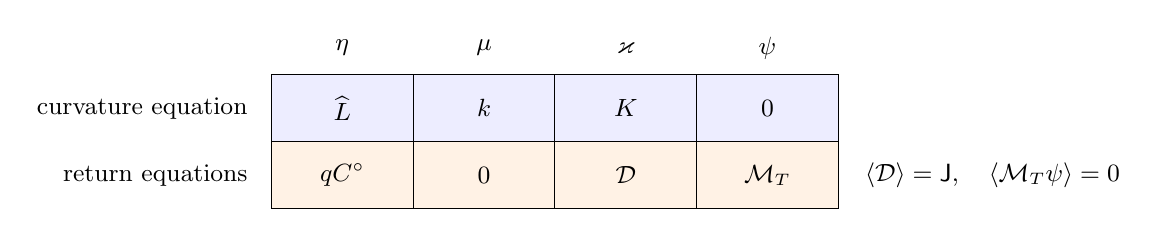
\begin{tikzpicture}[x=1.8cm,y=.85cm,font=\small]
\fill[blue!7] (0,1) rectangle (4,2);
\fill[orange!10] (0,0) rectangle (4,1);
\draw (0,0) rectangle (4,2);
\draw (0,1)--(4,1);
\foreach \x in {1,2,3} {\draw (\x,0)--(\x,2);}
\node at (.5,2.4) {$\eta$}; \node at (1.5,2.4) {$\mu$};
\node at (2.5,2.4) {$\varkappa$}; \node at (3.5,2.4) {$\psi$};
\node at (.5,1.5) {$\widehat L$}; \node at (1.5,1.5) {$k$};
\node at (2.5,1.5) {$K$}; \node at (3.5,1.5) {$0$};
\node at (.5,.5) {$qC^\circ$}; \node at (1.5,.5) {$0$};
\node at (2.5,.5) {$\mathcal D$}; \node at (3.5,.5) {$\mathcal M_T$};
\node[anchor=east] at (-.1,1.5) {curvature equation};
\node[anchor=east] at (-.1,.5) {return equations};
\node[anchor=west] at (4.12,.5)
 {$\av{\mathcal D}=\mathsf J,\quad\av{\mathcal M_T\psi}=0$};
\end{tikzpicture}
\caption{The corrected linear system and its four columns: the
increments $\eta,\mu,\varkappa,\psi$ of the height, of $\nu$, of the
controls $\kappa$ and of the charts. Taking the mean of the second
row removes the chart column. The feedback from the second row to the
height is multiplied by $q$.}
\label{fig:coupled-columns}
\end{figure}

\subsection{The control column gains all coefficient weights}

Let $G_{\bx}$ be the inverse of
Proposition~\ref{prop:rewrite-volume-inverse} and put
$U_{\bx}=G_{\bx}K_{\bx}$: the response $(\eta,\mu)$ of the first
equation to an increment of the controls. The natural space for
increments of the controls is
\[
 B_\beta=\Bigl\{\varkappa=(\varkappa_m):\
 \|\varkappa\|_{B_\beta}^2=\sum_mH_m^{-2\beta}|\varkappa_m|^2<\infty\Bigr\},
\]
which has no weight $M$ at all.

\begin{lemma}[Smoothing by the control column]\label{lem:control-smoothing}
For every $s$, with a fixed loss $d_*$,
\begin{equation}\label{eq:weak-control-smoothing}
 \|K_{\bx}\varkappa\|_{\mathcal Y_\beta,s}
 +\|U_{\bx}\varkappa\|_{\mathcal X_\beta,s}+|(U_{\bx}\varkappa)_{\mu}|
 \le C_s\,(1+\mathfrak n_{s+d_*})\,\|\varkappa\|_{B_\beta} ,
\end{equation}
where the middle term is the norm of the height component of
$U_{\bx}\varkappa$ and the last term is its scalar component.
\end{lemma}

\begin{proof}
\step{1: two decaying factors}
Differentiating the formula \eqref{eq:normalized-integral} for
$\mathcal F_q$ with respect to the controls gives
\[
 K_{\bx}\varkappa=\int_0^1D_\kappa\bigl[\,r\,D_z\mathcal N_{h}(h+tqu)\bigr]
 [\varkappa]\;u\,dt ,
\]
where $h'=w$ and the derivative $D_\kappa$ acts on $w$ and on $h$.
Every term of the result contains the increment of the control and a
derivative of positive order of the height $u$: the curvature
residual does not change when a constant is added to the height. This is true also at $q=0$, where
the derivative is that of $\mathscr L_wu$. On the component $m$ write
$\varkappa_m=H_m^\beta b_m$. The derivative of the height contributes
another factor $H_m^\beta$; the endpoint constant of $u$ does not
contribute, because the supports of the controls lie in negative
components. After division by the weight $H_m^\beta$ of the source
space a factor $H_m^\beta$ remains.

\step{2: summation}
At the order $s$, all coordinate, cutoff and reciprocal factors and
the derivatives of the control $\chi_m$ together cost a coefficient
power $\mathcal E_m^{C_s}$ and a fixed power of $M_m$; the remaining
factor $H_m^\beta$ bounds their product, by
\eqref{eq:full-material-envelope}. The product estimate
\eqref{eq:weighted-product} puts one factor of the state at the high
order. The supports of the controls are disjoint, so summing over $m$
gives the bound for $K_{\bx}$ with $(\sum_m|b_m|^2)^{1/2}
=\|\varkappa\|_{B_\beta}$. Composition with $G_{\bx}$ adds its fixed
loss.
\end{proof}

\subsection{Solving the corrected system}

\begin{proposition}[The approximate right inverse]\label{prop:approx-inverse}
After $\epsilon_0$ and the range of $q$ have been decreased, the
system \eqref{eq:corrected-coupled-linear-system} has for every
$(f,g)\in\mathfrak Y$ the solution
\begin{equation}\label{eq:joint-height-circle-inverse}
 \begin{split}
 \varkappa&=(I-q\,\mathsf J^{-1}R^\circ U)^{-1}\,
         \mathsf J^{-1}\,\bigl(\av g-q\,R^\circ Gf\bigr),\\
 (\eta,\mu)&=Gf-U\varkappa,\\
 \psi&=\mathcal M_T^{-1}\bigl(g-q\,C^\circ\eta-\mathcal D\varkappa\bigr),
 \end{split}
\end{equation}
where the subscript $\bx$ is omitted and $R^\circ$, $C^\circ$ act on
the height component of $G$ and $U$. The map
\[
 \mathbf V(\bx,q)\,(f,g)=(\eta,\mu,\varkappa,\psi\circ h_L)
\]
is smooth tame, and linear in $(f,g)$.
\end{proposition}

\begin{proof}
\step{1: elimination}
The first row gives $(\eta,\mu)=Gf-U\varkappa$. Taking the angular
mean of the second row removes $\mathcal M_T\psi$ and gives
\[
 (I-q\,\mathsf J^{-1}R^\circ U)\,\varkappa
              =\mathsf J^{-1}\,\bigl(\av g-q\,R^\circ Gf\bigr).
\]
By Lemma~\ref{lem:control-smoothing}, $R^\circ U$ is a bounded
operator from $B_\beta$ to the \emph{same} space $B_\beta$, with norm
controlled by finitely many norms of the state. Choose the
neighbourhood so that these norms are bounded, and then $|q|$ so small
that $\|q\,\mathsf J^{-1}R^\circ U\|_{B_\beta\to B_\beta}<\tfrac12$.
This gives the first line of
\eqref{eq:joint-height-circle-inverse}, and the second follows. By
the equation for $\varkappa$, the argument of $\mathcal M_T^{-1}$ in
the third line has mean zero on every component, so
\eqref{eq:rewrite-circle-inverse} applies.

\step{2: regularity}
Higher norms of $\varkappa$ are read off from the identity
\[
 \varkappa=\mathsf J^{-1}\bigl(\av g-q\,R^\circ Gf\bigr)
      +q\,\mathsf J^{-1}R^\circ U\varkappa ,
\]
satisfied by the solution already found. By
Lemma~\ref{lem:control-smoothing} the last term has all higher norms,
bounded by $\|\varkappa\|_{B_\beta}$ and one high norm of the state;
the first term has the norms of the sources with a fixed loss. So
$\varkappa$ lies in all the spaces $\mathcal K_{\beta,s}$, with tame
bounds, and substitution gives the estimates for $\eta$, $\mu$ and
$\psi$.

\step{3: smoothness}
The resolvent identity gives continuity in the base space, and the
identity of Step~2 with its estimates gives continuity in every
order. By Theorem~\ref{thm:hamilton-inverse} below, applied to the
inverse in the first line, all three formulas are smooth tame.
\end{proof}

\subsection{The quadratic error and the Nash--Moser theorem}

We use two theorems of Hamilton. Tame spaces and smooth tame maps
were defined in Section~\ref{subsec:spaces}.

\begin{theorem}[Hamilton: families of inverses]
\label{thm:hamilton-inverse}
Let $U$ be an open subset of a tame space, let
$\mathfrak H,\mathfrak K$ be tame spaces, and let
$L:U\times\mathfrak H\to\mathfrak K$ be a smooth tame map which is
linear in its second argument. Suppose that $L(x)$ is bijective for
every $x\in U$, and that the family of inverses
$(x,y)\mapsto L(x)^{-1}y$ is continuous and tame. Then this family is
smooth tame.
\end{theorem}

This is \cite[Part~II, Theorem~3.1.1]{Hamilton1982}. Existence,
uniqueness, continuity and tame bounds for the inverses are
hypotheses; the theorem supplies their derivatives. It was used in
this way in Propositions~\ref{prop:rewrite-volume-inverse}
and~\ref{prop:approx-inverse}.

\begin{theorem}[Hamilton: implicit function theorem with quadratic error]
\label{thm:hamilton-quadratic}
Let $\mathfrak X,\mathfrak P,\mathfrak Y$ be tame spaces and let
$\mathbf R:U\subset\mathfrak X\times\mathfrak P\to\mathfrak Y$ be a
smooth tame map on an open set. Suppose there are smooth tame maps
$\mathbf V(\bx,q)\,\mathbf y$ with values in $\mathfrak X$, linear in
$\mathbf y\in\mathfrak Y$, and $\mathbf Q(\bx,q)\,[\mathbf r,\mathbf y]$
with values in $\mathfrak Y$, bilinear in
$(\mathbf r,\mathbf y)\in\mathfrak Y\times\mathfrak Y$, such that
\begin{equation}\label{eq:rewrite-hamilton-hypothesis}
 D_{\bx}\mathbf R(\bx,q)\,\mathbf V(\bx,q)\,\mathbf y
        =\mathbf y+\mathbf Q(\bx,q)\,[\mathbf R(\bx,q),\mathbf y]
\end{equation}
for all $(\bx,q)\in U$ and all $\mathbf y$. Then near every zero
$(\bx_0,q_0)$ of $\mathbf R$ there is a smooth tame map
$q\mapsto\bx(q)$ with $\bx(q_0)=\bx_0$ and
$\mathbf R(\bx(q),q)=0$.
\end{theorem}

This is \cite[Part~III, Theorem~3.3.1]{Hamilton1982}. The point of
the hypothesis is that $\mathbf V$ need only be an inverse \emph{up to
an error proportional to the residual}; but the identity must hold
exactly, with the two arguments of $\mathbf Q$ independent. An
informal quadratic bound would not suffice. The theorem gives a
solution, not its uniqueness, which we do not need.

\begin{proposition}[The quadratic error identity]\label{prop:quadratic-error}
For $\mathbf r=(\mathbf r_1,\mathbf r_2)\in\mathfrak Y$ and
$\mathbf y=(f,g)\in\mathfrak Y$, let $(\eta,\mu,\varkappa,\psi)$ be
given by \eqref{eq:joint-height-circle-inverse} and define
\[
 \mathbf Q(\bx,q)\,[\mathbf r,\mathbf y]
 =\Bigl(q\,\partial_\theta\bigl(B\,\mathbf r_1\,\eta_\theta\bigr)
                   +\mathscr E_{\bx}(\mathbf r_2)\,\eta,\ \
              \mathcal Q_h(\mathbf r_2,\psi)\Bigr),
\]
where in $\mathcal Q_h$ the points of evaluation in
\eqref{eq:full-height-chart-derivative} are those of the actual state
and only the explicit factors $\mathfrak e$, $\mathfrak e'$ are
replaced by $\mathbf r_2$, $\mathbf r_2'$, as was done for
$\mathscr E_{\bx}$ in
Proposition~\ref{prop:optical-residual-completion}. Then $\mathbf Q$
is a smooth tame family of bilinear maps
$\mathfrak Y\times\mathfrak Y\to\mathfrak Y$, and
\eqref{eq:rewrite-hamilton-hypothesis} holds.
\end{proposition}

\begin{proof}
For the increments \eqref{eq:joint-height-circle-inverse}, the
identities \eqref{eq:readable-completed-height-derivative} and
\eqref{eq:full-height-chart-derivative} give the true derivative
\begin{equation}\label{eq:joint-height-circle-quadratic-error}
 D_{\bx}\mathbf R\,(\eta,\mu,\varkappa,\psi\circ h_L)
 =\Bigl(f+q\,\partial_\theta\bigl(B\,\mathcal A\,\eta_\theta\bigr)
              +\mathscr E_{\bx}(\mathfrak e)\,\eta,\ \
        g+\mathcal Q_h(\mathfrak e,\psi)\Bigr),
\end{equation}
which is \eqref{eq:rewrite-hamilton-hypothesis} with
$\mathbf r=\mathbf R=(\mathcal A,\mathfrak e)$. The increments are
linear in $\mathbf y$, so $\mathbf Q$ is bilinear.

It takes values in $\mathfrak Y$. Its first component has integral
zero: one term is an angular derivative, the other is in divergence
form with compact support inside the negative components. Its second
component is even. Finally, every term is a product of two factors
each of which decays like $H^\beta$, so by the calculus of
Section~\ref{sec:fixed-geometry} and the estimates for flows,
$\mathbf Q$ is smooth tame with values in the spaces of weight
$\beta$. All neighbourhoods of the state used here are defined by
norms of one fixed finite order; their size does not depend on the
order of the output.
\end{proof}

\begin{theorem}[The solution branch]\label{thm:weak-branch}
There are $q_1>0$ and a smooth tame map
\begin{equation}\label{eq:rewrite-weak-branch}
 q\mapsto\bx(q)=(u_q,\nu_q,\kappa_q,h_{L,q}),\qquad |q|<q_1,
\end{equation}
with $\bx(0)=(\Phi_*,0,0,\id)$ and
$\mathbf R(\bx(q),q)=0$. In particular
$u_q=\Phi_*+O(q)$ in every norm of $\mathcal X_\beta$.
\end{theorem}

\begin{proof}
We verify the hypotheses of
Theorem~\ref{thm:hamilton-quadratic} with $\mathfrak P=\R$; they are
listed in Table~\ref{tab:hamilton-hypotheses}. The order of the
choices matters. First the reference profile, the spaces and the
finite order $b_0$ are fixed; then $\epsilon_0$; then the range of
$q$, so that the control equation in
Proposition~\ref{prop:approx-inverse} can be solved. All estimates of
higher order hold on the neighbourhood so obtained, with constants
that depend on the order; no further choice is made. At a zero of
$\mathbf R$ the identity \eqref{eq:rewrite-hamilton-hypothesis} shows
that the derivative with respect to the state is surjective, with
right inverse $\mathbf V$.
\end{proof}

\begin{table}[htbp]
\centering
\begin{tabularx}{\linewidth}{@{}lY@{}}
\toprule
Hypothesis & Where it is verified\\
\midrule
Tame spaces &
 Lemma~\ref{prop:full-physical-tame}; the scalar factors and the
 affine slice $\ell_*u=1$ are tame direct summands.\\
Open domain &
 The set $\mathfrak n_{b_0}<\epsilon_0$, defined by norms of one
 finite order
 (Lemma~\ref{lem:common-geometric-neighborhood},
 Proposition~\ref{prop:uniform-physical-geometry}).\\
$\mathbf R$ smooth tame, with values in $\mathfrak Y$ &
 Formula \eqref{eq:normalized-integral} and
 Lemma~\ref{lem:scalar-integral} for $\mathcal A$; the calculus of
 Lemmas~\ref{lem:one-high-factor}, \ref{lem:circle-flow}
 and~\ref{lem:current-geometric-jets} for $\mathfrak e$.\\
A zero &
 $(\bx_0,0)$: $\mathscr L_{w_*}\Phi_*=0$, $\ell_*\Phi_*=1$, and the
 reference return maps are rotations.\\
$\mathbf V$ smooth tame and linear &
 Proposition~\ref{prop:approx-inverse}, which rests on
 Proposition~\ref{prop:rewrite-volume-inverse}.\\
$\mathbf Q$ smooth tame and bilinear &
 Proposition~\ref{prop:quadratic-error}, with
 Proposition~\ref{prop:optical-residual-completion} for
 $\mathscr E_{\bx}$.\\
The identity \eqref{eq:rewrite-hamilton-hypothesis} &
 \eqref{eq:joint-height-circle-quadratic-error}.\\
\bottomrule
\end{tabularx}
\caption{The hypotheses of Theorem~\ref{thm:hamilton-quadratic} and
where they are verified.}
\label{tab:hamilton-hypotheses}
\end{table}


This solves the nonlinear system in the scale of weight $\beta$. The
next section extracts stronger information from the equations
themselves, without a second iteration in another space.

\section{The endpoint gain and the closed surface}
\label{sec:final-proof}

The branch of Theorem~\ref{thm:weak-branch} was constructed with the
weight $H^\beta$, because the reference inverse is available only for
exponents below one. This already suffices for the geometry: every
element of $\mathcal X_\beta$ is flat at the endpoints. In this
section we first show that the corrections to the metric are in fact
of size $q^2H^{2\beta}$, which quantifies how the final metric
differs from the reference one, and then we state the annular theorem
in its precise form and prove Theorems~\ref{thm:annulus-intro}
and~\ref{thm:main}.

The gain comes from two identities for angular means. The first
recovers the mean of the height from an expression which is quadratic
in the oscillating part. The second recovers the controls $\kappa$
from that mean and from another quadratic expression. A product of
two factors of size $H^\beta$ has size $H^{2\beta}$, and
$2\beta>1$. No new iteration in a stronger space is needed. In this
section a quantity of size $H^\beta$ is called \emph{weak} and one of
size $H^{2\beta}$ \emph{strong}; both are flat at the endpoints.

\subsection{Two identities for means}

\paragraph{The mean of the height.}
Let $\mathfrak F_w(U)$ be the connection period
\eqref{eq:cart-mean-path-flux}. By
\eqref{eq:mean-period-derivative} its derivative at $U=0$ is
$w\av{U_r}$. Let
\begin{equation}\label{eq:posterior-period-bilinear}
 \mathcal B_{w,U}(v_1,v_2)
 =\int_0^1(1-t)\,D_U^2\mathfrak F_w(tU)[v_1,v_2]\,dt
\end{equation}
be its Taylor remainder of second order. For a solution the period
vanishes identically, because its radial derivative is the mean of the
residual and it is zero at the endpoints. Hence, with
$u^{\rm av}=\av u$,
\begin{equation}\label{eq:mean-recovered-derivative}
 0=\mathfrak F_w(qu)=q\,w\,(u^{\rm av})'
   +q^2\,\mathcal B_{w,qu}(u,u),
 \qquad\text{that is,}\qquad
 (u^{\rm av})'=-\frac qw\,\mathcal B_{w,qu}(u,u) .
\end{equation}

\paragraph{The mean of the return residual.}
Use the additive coordinates $\mathbf v=(Z,\kappa,a)$ with $Z=qu$
and $h_L=\id+a$, and put
\[
 \mathcal C(\mathbf v)=\av{\mathfrak e(\mathbf v)},
 \qquad
 \mathcal B^\circ_{\mathbf v}(v_1,v_2)
 =\int_0^1(1-t)\,D^2\mathcal C(t\mathbf v)[v_1,v_2]\,dt .
\]
By Section~\ref{sec:solving-the-equation} the derivative of
$\mathcal C$ at $\mathbf v=0$ is the identity on $\kappa$, zero on
the odd increments of the charts, and $R_0^\circ$ on the mean of the
height. At a solution therefore
\begin{equation}\label{eq:weak-posterior-control}
 0=\kappa+q\,R_0^\circ u^{\rm av}
       +\mathcal B^\circ_{\mathbf v}(\mathbf v,\mathbf v) .
\end{equation}

Formulas \eqref{eq:mean-recovered-derivative} and
\eqref{eq:weak-posterior-control} already explain the exponent
$2\beta$. What remains is to verify the corresponding estimates in
the stronger topology, with all derivatives in the parameter, so that
the conclusion holds for the whole branch.

\subsection{Two weak factors give one strong remainder}

Fix a convex neighbourhood of $(U,\nu,\kappa,a)=(0,0,0,0)$ in the
spaces of weight $\beta$, small in one norm of finite order, on which
$D$ and $Q/w$ are positive and the charts are uniformly increasing.
Both Taylor remainders above are integrals over segments in this
neighbourhood; the map $\mathcal C$ does not depend on $\nu$.

\begin{lemma}[Quadratic remainders in the doubled weight]
\label{lem:posterior-two-weight}
The maps $(w,U,v_1,v_2)\mapsto w^{-1}\mathcal B_{w,U}(v_1,v_2)$ and
$(\mathbf v,v_1,v_2)\mapsto\mathcal B^\circ_{\mathbf v}(v_1,v_2)$
are smooth tame with values in the space $\mathcal X^0_{2\beta}$ of
radial functions and in $\mathcal K_{2\beta}$, respectively. For every
number $k$ of derivatives with respect to the state there is a loss
$d_k$, independent of the order $s$, such that
\begin{equation}\label{eq:posterior-multilinear-bound}
 \begin{split}
 &\bigl\|D^k\mathcal B[\eta_1,\ldots,\eta_k]\,
                         (\eta_{k+1},\eta_{k+2})\bigr\|_{2\beta,s}\\
 &\quad\le C_{s,k}\Bigl[\,
   \sum_{i=1}^{k+2}\|\eta_i\|_{s+d_k}
                    \prod_{j\ne i}\|\eta_j\|_{b+d_k}
   +(1+\|\mathbf y\|_{s+d_k})
                    \prod_j\|\eta_j\|_{b+d_k}\Bigr],
 \end{split}
\end{equation}
where $\mathcal B$ is either of the two maps, $\mathbf y$ is the
state, the norms of the arguments are those of weight $\beta$, and
compact scalars are measured by their absolute values. The same bound
holds for all derivatives of $\mathcal C$ of order at least two.
\end{lemma}

\begin{proof}
\step{1: counting weak factors}
On the component $m$, every increment of a control or of a chart, and
every derivative of positive order of a height, carries a factor
$H_m^\beta$. The endpoint constants of heights are harmless: only
derivatives of positive order enter, and those of $\chi_L$ are
supported in a compact positive region and vanish on the supports of
all controls on negative components. Differentiation does not
destroy a weak factor: for $u=H^\beta\widetilde u$,
\[
 H^{-\beta}\,\Dr u=\Dr\widetilde u+\beta\,(\Dr\log H)\,\widetilde u ,
\]
and $\Dr\log H$ is bounded. Products and restrictions to the pieces
cost fixed numbers of derivatives and reference factors
$\mathcal E_m^{C_{s,k}}$. So it suffices to show that every term of
the expressions in question contains two weak factors, one from each
of the two distinguished arguments: these give the weight
$H_m^{2\beta}$ of the output; the highest derivative is placed on one
argument or on one coefficient of the state; the complete product of
coefficients is absorbed into one power of $M$; and finite overlap
together with $\|ab\|_{\ell^2}\le\|a\|_{\ell^2}\|b\|_{\ell^\infty}$
sums over the components.

\step{2: the period}
With $k=w+U_r$, $p=U_\theta/r$ and $E=1+w^2$, the integrand of
$\mathfrak F_w(U)$ is
\[
 \frac{1+kp_\theta/(1-p^2)}{\sqrt{E(1-p^2)-k^2}}-1 ,
\]
a smooth function of $w$ and of the derivatives
$(U_r,U_\theta/r,U_{\theta\theta}/r)$ on the neighbourhood. Each
second derivative with respect to $U$ contains one such derivative
from each argument, and further differentiation with respect to the
state does not remove them. The factor
$w^{-1}=w_*^{-1}\exp(-\nu\chi_*-\sum_m\kappa_m\chi_m)$ is part of the
product of coefficients; it costs a coefficient power, not an
endpoint exponent.

\step{3: flows}
For the map $\mathcal C$ consider a normalized characteristic flow
$\dot\Theta=G(t,\Theta;\mathbf y)$, in the form
\eqref{eq:fixed-strip-root-flow} near a root. Its first and second
variations with respect to the state satisfy
\[
 \dot\Theta_i=G_\theta\,\Theta_i+G_i,
 \qquad
 \dot\Theta_{12}=G_\theta\,\Theta_{12}
   +G_{\theta\theta}\,\Theta_1\Theta_2
   +(G_1)_\theta\,\Theta_2+(G_2)_\theta\,\Theta_1+G_{12} .
\]
The integrating factor of the homogeneous equation is bounded above
and below, as in the proof of
Proposition~\ref{prop:uniform-physical-geometry}. The source $G_i$
contains one weak factor and $G_{12}$ two, so by variation of
constants $\Theta_i$ contains one and $\Theta_{12}$ two. Composition
of flows does not change the weight of the component.

\step{4: inverses}
If $\iota=h^{-1}$, then
\[
 \iota_i=-\frac{h_i\circ\iota}{h'\circ\iota},\qquad
 \iota_{12}=-\frac{h_{12}\circ\iota
 +(h_1'\circ\iota)\,\iota_2+(h_2'\circ\iota)\,\iota_1
 +(h''\circ\iota)\,\iota_1\iota_2}{h'\circ\iota} .
\]
The denominator is bounded below, and every term of the second
numerator contains both variations. Apply this to $f^{-1}$ and
$h_R^{-1}$ in \eqref{eq:full-height-one-chart}; taking even or odd
parts and means preserves the weights.

\step{5: higher variations}
Label the directions of differentiation by a finite set $I$. In the
chain rule for $G(t,\Theta;\mathbf y)$, a subset $J\subset I$ acts
directly on the state and the blocks $B$ of a partition of
$I\setminus J$ act on the flow, giving terms
\[
 \bigl(D_{\mathbf y}^{|J|}\partial_\theta^{\ell}G\,
                   [\eta_j:j\in J]\bigr)\circ\Theta\;
                            \prod_{B}\Theta_B ,
\]
where $\ell$ is the number of blocks. Keep the term
$G_\theta\,\Theta_I$ on the left side; all other terms involve only
variations of lower order and contain every label exactly once. By
induction both distinguished factors are retained, and the identity
for inverses has the same structure. The additional weak factors are
bounded in low norms. The tame estimates for products and
compositions put only one factor at the high order, and the formulas
for the coefficients, the regularization at the roots and the
restrictions have fixed order; $k$ variations add a cost depending on
$k$ but not on $s$. This proves
\eqref{eq:posterior-multilinear-bound}.

\step{6: smoothness}
These are estimates for the actual derivatives. Taylor's formula with
integral remainder and one more variation gives continuity and
differentiability in the norms of weight $2\beta$, and by iteration
smoothness in the stronger Fr\'echet topology, not only pointwise
decay.
\end{proof}

\subsection{Recovering the mean and the controls}

\begin{lemma}[A primitive keeps the endpoint exponent]
\label{lem:weighted-primitive}
Let $\gamma>0$. For a radial function $f\in\mathcal X^0_\gamma$ let
$\mathscr Pf$ be its primitive which vanishes at the right endpoint.
Then $\mathscr Pf=v+a_L\chi_L$ with $v\in\mathcal X^0_\gamma$ and
$a_L\in\R$, and $\mathscr P:\mathcal X^0_\gamma\to\mathcal X_\gamma$
is a tame linear map on radial functions.
\end{lemma}

\begin{proof}
Near an endpoint, orient $\varrho$ towards it. Then
$(\log H)'\to-1$ in the variable $\varrho$, so far enough out
\[
 \frac{d}{d\varrho}\log H^\gamma\le-\frac\gamma2 :
\]
the ratio of $H^\gamma$ at $\sigma\ge\varrho$ to its value at
$\varrho$ is at most $e^{-\gamma(\sigma-\varrho)/2}$. Near the right
endpoint $\mathscr Pf(\varrho)=-\int_\varrho^\infty f\,\ell\,d\sigma$,
where the factor $\ell\le d_\partial$ comes from $dr=\ell\,d\varrho$
and is bounded. So the kernel of $\mathscr P$, conjugated by the
weight $H^{-\gamma}$, is bounded by $Ce^{-\gamma(\sigma-\varrho)/2}$
for $\sigma\ge\varrho$ and vanishes otherwise. Its integrals in
either variable are bounded, and Schur's test gives the bound in
$L^2(d\varrho)$. One derivative of the primitive is $\ell f$; further
derivatives with respect to $\varrho$ fall on $f$, on the weight and
on $\ell$, whose logarithmic derivatives are bounded. A factor $M^c$
with $c\ge0$ causes no loss, since $M(\varrho)\le M(\sigma)$ for
$\sigma\ge\varrho$. Near the left endpoint the same
argument applies to $\mathscr Pf-a_L$, where
$a_L=-\int_{r_-}^{r_+}f\,dr$ is a continuous functional of $f$,
because this difference is the primitive which vanishes at the left
endpoint. On the compact middle part integration is bounded in every
Sobolev norm, and the derivative of $\chi_L$ is supported there.
\end{proof}

\paragraph{The mean.}
By \eqref{eq:mean-recovered-derivative} the mean of the height on the
solution branch is given by the explicit map
\begin{equation}\label{eq:rewrite-mean-recovery}
 \mathcal U(\bx,q)
 =-q\,\mathscr P\bigl[w^{-1}\mathcal B_{w,qu}(u,u)\bigr],
 \qquad u_q^{\rm av}=\mathcal U(\bx(q),q) .
\end{equation}
By Lemma~\ref{lem:posterior-two-weight}, $\mathcal U$ is smooth with
values in $\mathcal X_{2\beta}$, and it is $O(q)$ in every norm; in
particular the difference of the endpoint values of $u_q$ is $O(q)$.

\paragraph{The controls.}
The operator $R_0^\circ$ of
\eqref{eq:rewrite-reference-circle-row} involves only the derivative
of its argument. It maps the part of $\mathcal U$ in
$\mathcal X^0_{2\beta}$ to $\mathcal K_{2\beta}$ with a fixed loss,
and annihilates the multiple of $\chi_L$, whose derivative is
supported in a positive component. By
\eqref{eq:weak-posterior-control},
\begin{equation}\label{eq:rewrite-control-recovery}
 \kappa_q=-q\,R_0^\circ\,\mathcal U(\bx(q),q)
            -\mathcal B^\circ_{\mathbf v(q)}(\mathbf v(q),\mathbf v(q)) .
\end{equation}
Since $\mathbf v(q)=O(q)$ on the branch, both terms on the right are
$O(q^2)$ in every norm of $\mathcal K_{2\beta}$. The identity also
shows that $q\mapsto\kappa_q$ is smooth with values in
$\mathcal K_{2\beta}$, and that $\dot\kappa_0=0$, where the dot
denotes the derivative with respect to $q$.

\paragraph{The compact parameter.}
Differentiating the equation $\mathcal F_q(w_q,u_q)=0$ at $q=0$,
\[
 \mathscr L_{w_*}\dot u_0+\dot\nu_0\,k_*+K_*\,\dot\kappa_0
       +\partial_q\mathcal F_q(w_*,\Phi_*)\big|_{q=0}=0,
 \qquad \ell_*\dot u_0=0 .
\]
The last term is quadratic in the derivatives of $\Phi_*$, which
contain only the angular frequency two; products of $\cos2\theta$ and
$\sin2\theta$ contain only the frequencies zero and four. So this
term has no component in the second mode. Since also
$\dot\kappa_0=0$, the second mode of the equation is the homogeneous
bordered equation of Proposition~\ref{prop:rad-fixed-theorem}, whose
only solution is zero. Hence $\dot\nu_0=0$ and $\nu_q=O(q^2)$.

\begin{figure}[htbp]
\centering
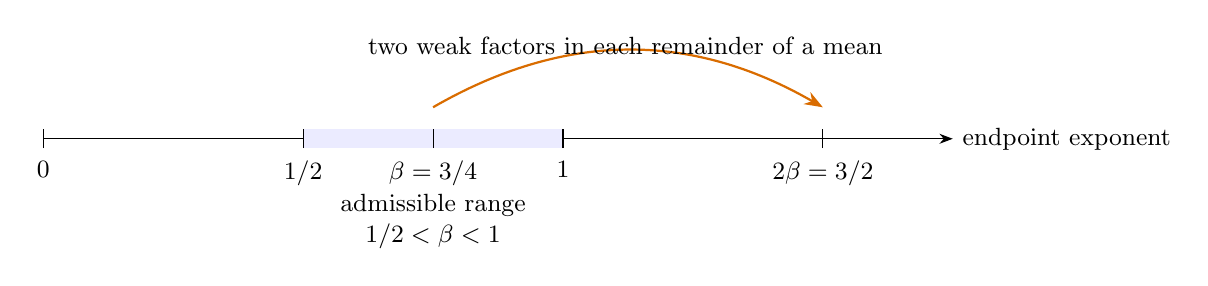
\begin{tikzpicture}[x=6.6cm,y=1cm,font=\small,>=Stealth]
\draw[->] (0,0)--(1.75,0) node[right] {endpoint exponent};
\fill[blue!8] (.5,-.12) rectangle (1,.12);
\foreach \x/\lab in {0/0,.5/{1/2},.75/{\beta=3/4},1/1,1.5/{2\beta=3/2}}
 {\draw (\x,-.12)--(\x,.12); \node[below] at (\x,-.16) {$\lab$};}
\draw[->,thick,orange!85!black] (.75,.4) to[bend left=30] (1.5,.4);
\node[above] at (1.12,.95) {two weak factors in each remainder of a mean};
\node[align=center] at (.75,-1.05) {admissible range\\$1/2<\beta<1$};
\end{tikzpicture}
\caption{The two roles of the exponent $\beta=\tfrac34$. Exponents
near $\beta$ and below one are needed for the reference inverse. The
equations for the means multiply two factors of weight $\beta$ and
give an exponent above one, which yields the bound for the metric in
Theorem~\ref{thm:new-annular-height}. Flatness of the solution needs
only a positive exponent.}
\label{fig:exponent-gain}
\end{figure}

\subsection{The annular theorem}

For a profile $w$ let $h_w$ denote the radial function with
$h_w'=w$, with a fixed normalization of the additive constant.

\begin{theorem}[A nonradial height with flat ends]
\label{thm:new-annular-height}
Let $w_*$, $\phi_*$, $\chi_*$ be as in
Proposition~\ref{prop:rad-fixed-theorem} and let $\chi_m$ be the
controls of Lemma~\ref{lem:quantitative-optical-controls}. There are
$q_0>0$ and a smooth family
\[
 (u_q,\nu_q,\kappa_q,h_{L,q}),\qquad |q|<q_0,
\]
through $(\Phi_*,0,0,\id)$ at $q=0$, such that the profile and the
height
\[
 w_q=w_*\exp\Bigl(\nu_q\chi_*+\sum_m\kappa_{q,m}\chi_m\Bigr),
 \qquad z_q=h_{w_q}+q\,u_q
\]
have the following properties, where
$g_q=(1+w_q^2)\,dr^2+r^2\,d\theta^2$.
\begin{enumerate}
\item \textup{(Equation.)} $|dz_q|_{g_q}<1$ and
 $g_q-dz_q\otimes dz_q$ is flat; equivalently
 $\mathcal N_{h_{w_q}}(z_q)=0$ with $D>0$.
\item \textup{(Profile.)} $w_q>0$ on $(r_-,r_+)$, and $w_q$ extends
 smoothly by zero across both endpoints. The zeros of $w_q'$ are
 those of $w_*'$, and $w_q=w_*$ near each of them.
\item \textup{(Height.)} $z_q$ is even and $\pi$-periodic in
 $\theta$, and has a constant extension at each endpoint; the two
 constants may differ. Moreover $\ell_*u_q=1$, so $z_q$ is not
 radial for $q\ne0$.
\item \textup{(Returns.)} On every negative component $m$, the two
 characteristic return maps $f_{q,m,\pm}$ of the linearized equation
 at $z_q$ satisfy
 \begin{equation}\label{eq:annular-return-condition}
  h_{R,q,m}\circ f_{q,m,\pm}\circ h_{L,q,m}^{-1}=R_{\pm T_m}
 \end{equation}
 for odd increasing charts commuting with the translation by $\pi$,
 where $T_m$ is the travel angle of $w_*$.
\item \textup{(Estimates.)} For every $s$,
 \begin{equation}\label{eq:annular-branch-estimates}
  \|u_q-\Phi_*\|_{\mathcal X_\beta,s}\le C_s\,|q|,\qquad
  |\nu_q|+\|\kappa_q\|_{\mathcal K_{2\beta},s}\le C_s\,q^2 ,
 \end{equation}
 and the family is smooth in $q$ for these topologies. In particular,
 for all $a\ge0$ and $\epsilon>0$,
 \[
  |\partial_r^a(w_q-w_*)|\le C_{a,\epsilon}\,q^2\,H^{1-\epsilon}
 \]
 near the endpoints, and $w_q-w_*=O(q^2)$ in every $C^a$ norm.
\end{enumerate}
\end{theorem}

\begin{proof}
The family is the branch of Theorem~\ref{thm:weak-branch}. Choose
$q_0$ so that $[-q_0,q_0]$ lies in its domain; every seminorm of the
branch is bounded on this compact interval, with constants depending
on the order but with $q_0$ independent of the order.

\emph{Estimates.} The first bound in
\eqref{eq:annular-branch-estimates} is contained in
Theorem~\ref{thm:weak-branch}; the second and the smoothness in the
stronger topology follow from
\eqref{eq:rewrite-mean-recovery}, \eqref{eq:rewrite-control-recovery}
and the bound for $\nu_q$. On the tails $\chi_*$ vanishes, and
differentiating the formula for $w_q$ gives
$|\partial_r^a(w_q-w_*)|\le C_a\,q^2\,H^{2\beta}E_0^{C_a}$; since
$2\beta>1$, \eqref{eq:full-material-envelope} gives the stated bound.
On the compact middle part use the smoothness of the family and
$\nu_q=O(q^2)$.

\emph{Profile.} The controls vanish near every turning circle, so the
germ of the metric there is unchanged, and by
Proposition~\ref{prop:uniform-physical-geometry}(i) the sign of
$w_q'$ is that of $w_*'$ elsewhere. Flatness of $w_q$ follows from
that of $w_*$ and of the controls.

\emph{Equation and returns.} At a zero of $\mathbf R$ both residual
corrections vanish, so $\widehat L$ is the true linearization and its
exact returns are \eqref{eq:annular-return-condition}. The inequality
$D>0$ of Proposition~\ref{prop:uniform-physical-geometry}(i) is
equivalent to $|dz_q|_{g_q}<1$, and $\mathcal A=0$ means that the
curvature residual vanishes, which by
Proposition~\ref{prop:scalar-core} is the flatness of the remainder
metric.

\emph{Height.} The symmetry is that of the function spaces. Since
$\ell_*u_q=1$, the second angular mode of $u_q$ is not zero. By
Lemma~\ref{prop:full-physical-tame} every element of
$\mathcal X_\beta$ has constant extensions at the endpoints; the same
holds for all derivatives in $q$. Finally $h_{w_q}$ has constant
extensions because $w_q$ is flat.
\end{proof}

\subsection{Proof of Theorems~\ref{thm:annulus-intro} and~\ref{thm:main}}

The construction involves two parameters with different roles, and it
is worth separating them once more. The small parameter $q$ was used
to construct one nonradial isometric realization of one rotationally
symmetric metric. The phase $\tau$ moves that realization.

\begin{proof}[Proof of Theorem~\ref{thm:annulus-intro}]
Fix $q$ with $0<|q|<q_0$ and let $w=w_q$, $z=z_q$ be given by
Theorem~\ref{thm:new-annular-height}. Part~(i) of that theorem is
condition~(i); parts~(ii) and~(iii) give conditions~(ii) and~(iii).
\end{proof}

\begin{proof}[Proof of Theorem~\ref{thm:main}]
By Section~\ref{sec:geometric-closure},
Theorem~\ref{thm:annulus-intro} implies Theorem~\ref{thm:main}. In
detail: extend $w$ by zero and $z$ by its limiting constants to a
slightly larger annulus. The remainder metric is Euclidean on the
added collars, so the extended data satisfy the hypotheses of
Theorem~\ref{thm:geometric-closure}. That theorem develops the graph,
fills the inner disk, attaches the marked cap, and yields the family
\[
 F_\tau=R_{-2\pi\tau}\circ F\circ\varrho_{2\pi\tau}
\]
on the disk, with the inclusion on the cap. On the collars the two
rotations cancel pointwise; the marked cap makes two of the closed
images noncongruent; and the same theorem gives embeddedness and the
constancy of the area, of the enclosed volume and of the total
oriented mean curvature.
\end{proof}


\appendix
\section{Why a finite angular ansatz cannot work}
\label{app:app-obstructions}

This appendix is independent of the existence proof. It explains one
feature of the construction: although the seed $\Phi_*$ has the single
angular frequency two, the inverse of the linearized operator had to
be constructed for \emph{all} even frequencies.
Proposition~\ref{prop:obs-monotone-tail} ruled out a monotone flat end
for the linearized equation. Another tempting simplification would be
to look for the nonlinear height among functions with finitely many
angular modes. The following proposition shows that this is
impossible as soon as the height is required to be radial on a
collar.

\begin{proposition}\label{prop:obs-finite-square}
Let $E>0$ be a $C^1$ function on an interval $I\subset(0,\infty)$,
and let $z$ be a real $C^2$ solution of the Darboux equation
\eqref{eq:intro-darboux} for the metric $E\,dr^2+r^2\,d\theta^2$ on
$I\times\T$. Suppose that
\[
 z^2=\sum_{|j|\le J}b_j(r)\,e^{ij\theta},\qquad
 b_{-j}=\overline{b_j},\qquad b_j\in C^2(I),
\]
and that $z$ is independent of $\theta$ for $r$ in some nonempty open
subinterval of $I$. Then $z$ is independent of $\theta$ on all of
$I$.
\end{proposition}

The hypothesis covers every height with finitely many angular modes,
and every smooth square root of a trigonometric polynomial in
$\theta$.

The difficulty in the proof is the continuation through a zero of a
Fourier coefficient. The highest coefficient satisfies an ordinary
differential equation which is singular where the coefficient
vanishes, and the coefficient is complex, so neither the standard
uniqueness theorem nor an argument for real functions applies
directly.

\begin{proof}
\step{1: a polynomial identity for $v=z^2$}
Let $K=E'/(2rE^2)$ be the curvature of the metric. From
$\nabla^2v=2z\,\nabla^2z+2\,dz\otimes dz$ and the expansion of a
$2\times2$ determinant under a perturbation of rank one,
\begin{equation}\label{eq:obstruction-polynomial}
 2v\,\det\nolimits_g\nabla^2v
 -\operatorname{cof}_g(\nabla^2v)[dv,dv]
       =8Kv^2-2Kv\,|dv|_g^2 .
\end{equation}
Indeed, on the left the terms containing
$z^3\operatorname{cof}_g(\nabla^2z)[dz,dz]$ cancel, leaving
$8z^4\det_g\nabla^2z$, and the Darboux equation gives the right side.
No division by $z$ was used, so the identity holds also where $z=0$.

\step{2: the equation for the highest coefficient}
Let $b=b_J$ be the coefficient of the highest frequency $J>0$, and put
$a=EJ^2/r$ and $d=E'J^2/(2r)$. In \eqref{eq:obstruction-polynomial}
the frequency $3J$ arises only from products of three copies of
$b\,e^{iJ\theta}$. Write the entries of the Hessian of $v$ as
\[
 A=v_{rr}-\frac{E'}{2E}\,v_r,\qquad
 B=v_{r\theta}-\frac{v_\theta}r,\qquad
 C=v_{\theta\theta}+\frac rE\,v_r ,
\]
so that, after multiplication by $Er^2$, the left side of
\eqref{eq:obstruction-polynomial} is
$2v(AC-B^2)-(Cv_r^2-2Bv_rv_\theta+Av_\theta^2)$. Replacing
$v,v_r,v_{rr},v_\theta,v_{r\theta},v_{\theta\theta}$ by
$b,b',b'',iJb,iJb',-J^2b$ and including the cubic term of the right
side, the coefficient of $e^{3iJ\theta}$ gives
\begin{equation}\label{eq:obstruction-highest-mode}
\begin{split}
0={}&(2bb'-ab^2)\,b''-(b')^3+ab\,(b')^2
 -\frac{2a}{r}\,b^2b'+\frac{2a}{r^2}\,b^3\\
 &\quad+d\,b^2b'-\frac{2d}{r}\,b^3 .
\end{split}
\end{equation}
In particular $b'=0$ wherever $b=0$.

\step{3: a first-order system where $b\ne0$}
On a component of $\{b\ne0\}$ choose a continuous complex square root
$y$ of $b$. Substituting $b=y^2$ in
\eqref{eq:obstruction-highest-mode} and dividing by $2y^4$,
\begin{equation}\label{eq:obstruction-square-root}
 (4y'-ay)\,y''+a\Bigl(y'-\frac yr\Bigr)^2
 +d\Bigl(yy'-\frac{y^2}r\Bigr)=0 .
\end{equation}
Fix a compact subinterval of $I$ and a constant $K_1>1+\sup|a|$, and
consider
\[
 U=\max\bigl(K_1|y|,\,|y'|\bigr)
   =\max\Bigl(K_1\sqrt{|b|},\ \frac{|b'|}{2\sqrt{|b|}}\Bigr).
\]
We claim $|U'|\le CU$ almost everywhere. Where $|y'|\ge K_1|y|$ we
have $|4y'-ay|\ge3|y'|$, and \eqref{eq:obstruction-square-root} gives
$|y''|\le C|y'|$. Where $K_1|y|$ is the larger term, its derivative is
at most $K_1|y'|\le K_1U$ in absolute value. The maximum of two
Lipschitz functions is Lipschitz, so the estimate holds across the
points where the maximum switches. Consequently $U$ is bounded above
and bounded away from zero on the component, up to its endpoints in
the compact subinterval.

\step{4: zeros are isolated and quadratic}
Let $r_0$ be an endpoint, interior to $I$, of a component of
$\{b\ne0\}$. There $y\to0$, so $U=|y'|$ nearby, and since
$|y''|\le C|y'|$ the derivative $y'$ has a limit $\lambda$, which is
not zero because $U$ is bounded below. Hence
\begin{equation}\label{eq:obstruction-quadratic-zero}
 b''=2\,(y')^2+2\,y\,y''\longrightarrow2\lambda^2\ne0
 \qquad(r\to r_0).
\end{equation}
So $r_0$ is an isolated zero of $b$ of order exactly two. Across such
a zero $U$ extends continuously, with the value $\sqrt{|b''|/2}$, and
satisfies the same differential inequality.

\step{5: continuation}
Consider the open set
$\mathcal O=\{b\ne0\}\cup\{b=0,\ b''\ne0\}$. Suppose a component of
$\mathcal O$ had a boundary point in the interior of $I$; there
$b=b''=0$. If zeros of $b$ accumulated at this point from inside the
component, the lower bound for $U$ at these quadratic zeros and the
continuity of $b''$ would give a contradiction; if a last interval
of $\{b\ne0\}$ ended at this point,
\eqref{eq:obstruction-quadratic-zero} would give a contradiction.
Hence $\mathcal O$ is empty or equal to $I$. By assumption $z^2$ is
radial on an open interval, so $b$ vanishes there and
$\mathcal O\ne I$. Therefore $b=0$ on $I$.

\step{6: conclusion}
Removing the highest coefficient and repeating the argument, all
coefficients $b_j$ with $j\ne0$ vanish, so $z^2$ is radial. For each
$r$ the function $\theta\mapsto z(r,\theta)$ is continuous on the
circle with constant square, hence constant.
\end{proof}

The proposition does not say that a single angular mode is useless: a
single mode is exactly the right seed for the linearized problem. It
says that the nonlinear correction of the seed cannot stay within any
finite number of modes once it has to meet a radial collar.

\section{External results and the order of choices}
\label{app:dependencies}

The proof is self-contained except for the results listed in
Table~\ref{tab:external}. The table records each of them in the form
in which it is used, so that the reader can see exactly what is taken
from the literature. The rigidity and flexibility theorems quoted in
the introduction give context only; none of their conclusions is used.

\renewcommand{\arraystretch}{1.12}\setlength{\tabcolsep}{4pt}
\begin{longtable}{@{}p{.21\linewidth}p{.47\linewidth}p{.25\linewidth}@{}}
\caption{External results in the form used.}\label{tab:external}\\
\toprule
Result & Statement used & Where\\
\midrule
\endfirsthead
\toprule
Result & Statement used & Where\\
\midrule
\endhead
Gauss equation and structure equations &
 For a surface with metric $g$ and second fundamental form
 $\mathrm{II}$ in a three-manifold, $K_g=\overline K+\det_g\mathrm{II}$,
 with $\overline K$ the sectional curvature of the tangent plane. For
 an oriented orthonormal coframe with
 $d\eta_1=\alpha\wedge\eta_2$, $d\eta_2=-\alpha\wedge\eta_1$:
 $d\alpha=-K\,\eta_1\wedge\eta_2$. &
 Lemma~\ref{lem:darboux-invariant},
 Proposition~\ref{prop:scalar-core}\\
Primitives and coverings &
 A closed one-form on a simply connected domain is exact. A proper
 local diffeomorphism of the plane which is the identity outside a
 compact set is a diffeomorphism. &
 Lemma~\ref{lem:disk-development}\\
Ordinary differential equations &
 Existence, uniqueness and smooth dependence on data and parameters;
 Gronwall's inequality. &
 radial models, flows, Proposition~\ref{prop:obs-monotone-tail}\\
Quadratic forms \cite[Theorems~2.12, 2.13]{Teschl2009} &
 A closed quadratic form which is bounded below is the form of a
 unique self-adjoint operator. &
 the models of Section~\ref{sec:radial-models};
 Lemma~\ref{lem:radial-deep-inverse}\\
Spectral theorem \cite[Chapter~3]{Teschl2009} &
 For a self-adjoint operator $A$ and $z$ outside its spectrum,
 $\|(A-z)^{-1}\|=\dist(z,\sigma(A))^{-1}$. &
 Lemmas~\ref{lem:central-gap}, \ref{lem:morse-arithmetic}\\
Weyl's theorem \cite[Theorem~6.19]{Teschl2009} &
 If the difference of the resolvents of two self-adjoint operators
 is compact, their essential spectra coincide. &
 Section~\ref{subsec:morse}\\
Harmonic oscillator \cite[Section~8.3]{Teschl2009} &
 The operator $-\partial_x^2+\omega^2x^2$ on the line has the simple
 eigenvalues $(2n+1)\omega$, $n\ge0$, and no other spectrum. &
 Section~\ref{sec:worked-example},
 Lemma~\ref{lem:central-gap}\\
Countable products &
 A sequence in a countable product of compact intervals has a
 subsequence which converges in every coordinate. &
 Lemma~\ref{lem:radial-product-selection}\\
Three-lines lemma &
 A strongly analytic family of operators on $0<\operatorname{Re}z<1$,
 strongly continuous on the closed strip and bounded there on each
 vector, with operator norm bounds $M_0,M_1\ge0$ on its two boundary
 lines, is bounded by
 $M_0^{1-\vartheta}M_1^{\vartheta}$ on the line
 $\operatorname{Re}z=\vartheta$. &
 Lemma~\ref{lem:ang-base-inverse-regularity}\\
Extension operator &
 On a half-line or an interval there is a linear extension operator
 to the line which is bounded in every Sobolev norm. &
 after Lemma~\ref{lem:one-high-factor}\\
Hamilton's theorem on families of inverses &
 Theorem~\ref{thm:hamilton-inverse}. &
 Propositions~\ref{prop:rewrite-volume-inverse},
 \ref{prop:approx-inverse}\\
Hamilton's theorem with quadratic error &
 Theorem~\ref{thm:hamilton-quadratic}. &
 Theorem~\ref{thm:weak-branch}\\
\bottomrule
\end{longtable}

The Airy asymptotics \cite{DLMFAiry} quoted in
Section~\ref{sec:worked-example} serve as a heuristic only.

\paragraph{Two elementary facts used repeatedly.}
\emph{Schur's test.} If the blocks $K_{nm}$ of an operator matrix
satisfy $\sup_n\sum_m\|K_{nm}\|\le A$ and
$\sup_m\sum_n\|K_{nm}\|\le B$, then the operator is bounded on the
$\ell^2$ sum with norm at most $\sqrt{AB}$: apply the Cauchy--Schwarz
inequality with the weights $\|K_{nm}\|$ in each row, and then the
bound for the columns. \emph{Neumann series.} If $\|R\|<1$ on a
Banach space, then $\sum_{k\ge0}(-R)^k$ converges in norm to a
two-sided inverse of $I+R$. Whenever a Neumann series is used in this
paper, the space is one fixed Banach space and the bound $\|R\|<1$ is
established before any derivative of higher order is taken.

\paragraph{The order of the choices.}
The constants of the construction are chosen in the following order;
no later choice changes an earlier one.
\begin{enumerate}[label=\textup{\arabic*.}]
\item \emph{The models.} The parameters of the central oscillator and
 of the Morse models, the exponent $12$ of the joins and the
 constant $c_0$ of the matching angle
 (Sections~\ref{sec:radial-models}, \ref{sec:radial-tails}).
\item \emph{The profile.} The exponent $\ea$ of the source weight,
 then $C_*$, then the initial index $N$, then the cuts of the central
 model and the lengths of the cone heads; then the height ratios
 $\sigma_n$, by Lemma~\ref{lem:radial-product-selection}; then the
 connectors. These choices use only $|\gamma|\le1$ and are therefore
 the same for all endpoint exponents
 (Lemma~\ref{lem:radial-uniform-exponents}).
\item \emph{The reference inverse.} A compact interval of endpoint
 exponents $\gamma\in(0,1)$ changes the constants of the estimates,
 not the profile. The final border $(g_*,\ell_*)$ is fixed after the
 geometry (Section~\ref{subsec:final-border}).
\item \emph{The spaces.} The exponent $\beta=\tfrac34$, the collars
 $\delta_n^{\rm root}$, the controls $\chi_n$ and the cutoffs
 (Section~\ref{subsec:root-geometry}).
\item \emph{The neighbourhood.} The finite order $b_0$, then
 $\epsilon_0$, so that the comparisons of
 Lemma~\ref{lem:common-geometric-neighborhood} hold and the relative
 operator has norm less than $\tfrac12$ on one space
 (Lemma~\ref{lem:relative}).
\item \emph{The parameter.} The range of $q$, so that the control
 equation of Proposition~\ref{prop:approx-inverse} is solvable.
\end{enumerate}
Estimates of higher order change constants and use a fixed shift of
the order; they never require a new choice of the profile, of the
neighbourhood or of the range of $q$. The two inequalities
$\tfrac12<\beta<1$ serve different purposes: $\beta<1$ leaves room for
two neighbouring exponents at which the reference inverse is
available, and $\beta>\tfrac12$ makes the product of two decaying
factors decay faster than $H$.

\section{Index of notation}
\label{app:notation}

The tables list the symbols that are used in more than one place,
with the place where each is introduced. Letters not listed here have
a meaning local to one proof or one subsection, stated there. A few
letters are deliberately reused in different parts for unrelated
objects, as indicated.

\renewcommand{\arraystretch}{1.12}\setlength{\tabcolsep}{4pt}\raggedbottom

\subsection*{General, and Part~\ref{part:geometry}}

\begin{longtable}{@{}p{.23\linewidth}p{.52\linewidth}p{.19\linewidth}@{}}
\toprule
Symbol & Meaning & Introduced\\
\midrule
\endhead
$\T$, $\av f$, $R_\vartheta$ & circle $\R/2\pi\Z$; angular average;
 rotation by $\vartheta$ & \S\ref{subsec:conventions}\\
$e_j$ & $\sqrt2\cos(j\theta)$ & \S\ref{sec:rosen-reference-packet}\\
$w$, $h$, $E$, $g$ & profile (slope), radial height with $h'=w$,
 $E=1+w^2$, metric $E\,dr^2+r^2d\theta^2$ & \eqref{eq:intro-metric}\\
$z$, $u$, $q$ & height $z=h+qu$; small parameter & \S\ref{subsec:normalization}\\
$\bar g$ & remainder metric $g-dz\otimes dz$ & \S\ref{sec:geometric-closure}\\
$F_\tau$, $\tau$, $\varrho_\vartheta$ & the bending, its phase,
 intrinsic rotation & \eqref{eq:phase-family}\\
$k$, $p$, $D$, $Q$ & $z_r$, $z_\theta/r$, discriminant, $k+Ep_\theta$
 & \eqref{eq:height-jet-notation}\\
$\alpha$ & connection form of the remainder metric & \eqref{eq:conn-one-form}\\
$\mathcal N_h(z)$ & curvature residual & \eqref{eq:cart-curvature-scalar}\\
$\mathcal F_q(w,u)$, $\mathcal A$ & normalized residual
 & \eqref{eq:cart-removable-equation}\\
$a$, $b$, $c$ & coefficients of the linearization
 & \eqref{eq:linear-coefficients}\\
$\mathscr L_w$, $L_j$, $L'_{2,w}$ & linearization at the radial
 height; its $j$th mode; derivative in $w$
 & \eqref{eq:intro-linearization}, \eqref{eq:rad-eq-modal-operator}\\
$K_0$, $K_g$ & $ww'/r$; curvature of $g$
 & \eqref{eq:cart-determinant-identity}, \eqref{eq:radial-curvature}\\
$B$, $\bar c$, $\bar L$ & first residual correction
 & Lemma~\ref{lem:type-completion}\\
$d$, $v$, $c_\pm$ & drift, speed and slopes of characteristics
 & \eqref{eq:completed-characteristics}\\
$\mathfrak F_w$ & connection period & \eqref{eq:cart-mean-path-flux}\\
$T$, $T_m$ & travel angle of a negative component
 & \S\ref{subsec:layout}\\
\bottomrule
\end{longtable}

\subsection*{Part~\ref{part:reference}}

\begin{longtable}{@{}p{.23\linewidth}p{.52\linewidth}p{.19\linewidth}@{}}
\toprule
Symbol & Meaning & Introduced\\
\midrule
\endhead
$X$, $\mathcal P$, $\rho$, $V_0$, $\lambda$ & model coordinate,
 density, potential data, height of a model & Lemma~\ref{lem:liouville}\\
$H_{j,c}$, $H_{j,M}$ & Schr\"odinger operators of the central and
 Morse models & \S\ref{subsec:rad-central-singlepoint}, \S\ref{subsec:morse}\\
$\upsilon$ & $r_X/r$ & \eqref{eq:rad-eq-sc6}\\
$\varpi$, $d\mu$, $B_j$ & $12w/r^2$; $\varpi\,dr$; $-\varpi^{-1}L_j$
 & \eqref{eq:rad-eq-ha2}\\
$A_c$, $a_c$, $c_c$, $\alpha_c$, $\phi_0$ & constants and seed of the
 central model & \eqref{eq:rad-eq-sc1}, \eqref{eq:rad-eq-sc2}\\
$g_0$, $\ell_0$ & temporary border & \S\ref{subsec:rad-central-singlepoint}\\
$A$, $B$, $d$ & Morse parameters (in \S\S\ref{subsec:morse}--\ref{sec:radial-tails})
 & \eqref{eq:rad-eq-rm5}\\
$d_n$, $A_n$, $B_n$ & parameters of cell $n$; $A_n\asymp e^{-n^2}$
 & \S\ref{sec:radial-tails}\\
$\lambda_n$, $\sigma_n$ & height of cell $n$; height ratios
 & \eqref{eq:rad-eq-js2}\\
$S_n$, $H_n$, $q_n$, $\mathcal E_n$ & $\tfrac23n^3$, $e^{-S_n}$,
 $n^{5/2}\log(e+n)$, $e^{q_n}$ & \eqref{eq:rad-eq-endpoint-weights}\\
$M_n$ & $\exp\{1+n^{5/2}\log^2(e+n)\}$ & \eqref{eq:M-weight}\\
$N$, $C_*$, $c_0$ & first cell index; band constant; angle constant
 & \S\ref{sec:radial-tails}\\
$X_c$, $X_L$, $X_R$, $\mathfrak r_n$ & cut and roots of a cell;
 radius factor & \S\ref{subsec:one-cell}, \S\ref{subsec:joins}\\
$\tau_{n,j}$ & action $j\sqrt{A_n}$ of the caps of cell $n$
 & \eqref{eq:cap-action}\\
$\mathsf p_j$, $\Lambda$ & gauge density $wr^{2j^2-1}$;
 $j^2(j^2-1)$ (in \S\ref{sec:radial-tails}) & \eqref{eq:rad-eq-rm13}\\
$I_n$, $J_n$; $\mu_n,\nu_n,R_n^I,R_n$ & mass and resistance
 intervals; masses and resistances & \eqref{eq:mass-resistance-def-new}\\
$a_n$, $y_n$, $b_n$, $c_n$ & node values and coefficients of the
 recurrence & Lemma~\ref{lem:radial-deep-inverse}\\
$\jn_n$, $\mathcal I_n$ & band edges; frequency bands
 & \eqref{eq:rad-eq-rm21}\\
$\zeta_j$, $\Xi_n$, $\Upsilon_n$, $\delta_n$ & state variable on a
 join; height contrast; matching angle
 & \S\ref{subsec:height-selection}\\
$w_*$, $\phi_*$, $\chi_*$, $g_*$, $\ell_*$ & reference profile, seed,
 metric control, border & Prop.~\ref{prop:rad-fixed-theorem}\\
$\mathbb L_{w_*}$, $\mathbb G_{w_*}$ & bordered reference operator and
 its inverse & \eqref{eq:rad-eq-bordered-reference},
 Lemma~\ref{lem:rad-green-completion}\\
$Y_{\gamma,s}$, $\ea$, $\eb$, $\el$ & source norm; exponents of the
 coefficient allowance & \eqref{eq:rad-eq-source-norm},
 Lemma~\ref{lem:inner-inverse}\\
$\vartheta_m$, $\chi_L$ & partition of unity; endpoint step function
 & \S\ref{sec:radial-what}\\
$G_h$, $R_o$, $G$ & inner, outer and matched inverses
 & \eqref{eq:rad-eq-hn9}, \eqref{eq:outer-robin-new}, \eqref{eq:rad-eq-tm11}\\
$\mS$, $\mK$, $\mA$, $\mB$, $D_0$, $D_b$ & matching matrices
 & \S\S\ref{subsec:rad-localized-hilbert-assembly}--\ref{subsec:terminal-matching}\\
$\mathcal K_n$ & transfer bound $e^{Cn^2+C_o\tau_{n,j}}$
 & \eqref{eq:transition-inputs-new}\\
$\mathcal D^{\rm rad}_\gamma$ & weighted graph domain
 & Def.~\ref{def:radial-graph-domain}\\
\bottomrule
\end{longtable}

\subsection*{Part~\ref{part:nonlinear}}

\begin{longtable}{@{}p{.23\linewidth}p{.52\linewidth}p{.19\linewidth}@{}}
\toprule
Symbol & Meaning & Introduced\\
\midrule
\endhead
$x_\partial$, $H$, $E_0$, $M$ & continuous versions of the endpoint
 scales & \eqref{eq:readable-physical-weights}\\
$\ell$, $\varrho$, $\Dr$ & unit-scale radial variable and derivative
 & \S\ref{subsec:spaces}\\
$\beta$, $\epsilon$ & weight exponent $\tfrac34$; gap between
 exponents & \eqref{eq:beta-choice}, \S\ref{subsec:two-exponents}\\
$\mathcal X_\gamma$, $\mathcal X_\gamma^0$, $\mathcal Y_\beta$,
$\mathcal Z_\gamma$, $\mathcal K_\gamma$, $\Qint$ & spaces of heights,
 sources, circle data; integral functional
 & Def.~\ref{def:readable-physical-grading}\\
$\bx=(u,\nu,\kappa,h_L)$, $\Phi_*$ & state; reference height
 $\phi_*e_2$ & \eqref{eq:rewrite-state}\\
$\chi_m$ & travel-angle controls
 & Lemma~\ref{lem:quantitative-optical-controls}\\
$\mathfrak n_s$, $\mathfrak g_{s,m}$; $b_0$, $\epsilon_0$, $d_*$ &
 seminorms of the state; the neighbourhood; fixed loss
 & \S\ref{subsec:neighbourhood}\\
$f$, $h_R$, $\mathfrak e$ & minus return map, right chart, return
 residual & \eqref{eq:full-height-one-chart}\\
$\mathcal M_T$, $\mathcal Q_h$ & derivative of $\mathfrak e$ in the
 chart & \eqref{eq:full-height-chart-derivative}\\
$\widehat L$, $\mathscr E_{\bx}$ & corrected linearization; its error
 & Prop.~\ref{prop:optical-residual-completion}\\
$\sigma$, $\varphi$; $\xi_L$, $\xi_R$, $\xi_c$ & travel coordinates;
 root coordinates & \eqref{eq:fixed-strip-coordinates}\\
$W_i$, $h_i$, $\alpha_i$, $V_i$ & canonical unknown, height factor,
 density, potential & \eqref{eq:fixed-strip-airy-equation}\\
$y$, $\bd$, $P_{\bx}$, $P_*$ & positive coordinate; $y(1-y)$;
 positive canonical operators & \S\ref{subsec:positive-crossing}\\
$\mathscr C_{\bx}$, $\mathscr S_{\bx}$, $\mathbb L_{\bx}$ &
 transformations to canonical form & \S\ref{subsec:canonical-problem}\\
$\mathbb V_{t,s}$ & spaces of canonical sources
 & \eqref{eq:vol-source-spaces}\\
$\mathbb P_{\bx}$, $\bW=(W,a_L,\mu,\lambda)$ & augmented operator and
 unknown & \eqref{eq:vol-abstract-complete-operator}\\
$k_{\bx}$, $s_{\bx}$, $c_*$ & columns of the augmented operator
 & \S\ref{subsec:canonical-problem}\\
$\mathbb G_*$, $\mathbb D_*$, $L_0$ & reference inverse, its domain,
 its loss & Lemma~\ref{lem:two-weights-closed-domain}\\
$|v|_{\mathcal F}$ & $L^1$ norm of the Fourier transform
 & Lemma~\ref{lem:one-high-factor}\\
$\mathfrak g_{s,m}$, $\mathfrak n_{s,m}$ & localized seminorms of the
 deformation and of the state & \S\ref{subsec:neighbourhood}\\
$\delta_n^{\rm root}$ & width of the root collars
 & \eqref{eq:geometry-root-collar-width}\\
$\mathscr R_{\bx}$ & relative operator & \S\ref{subsec:relative}\\
$G_{\bx}$ & inverse at a nearby state
 & Prop.~\ref{prop:rewrite-volume-inverse}\\
$\mathbf R$, $\mathbf V$, $\mathbf Q$ & residual, approximate inverse,
 quadratic error & \S\ref{sec:solving-the-equation}\\
$\mathfrak X$, $\mathfrak Y$ & spaces of increments and residuals
 & \S\ref{sec:solving-the-equation}\\
$C^\circ$, $R^\circ$, $\mathcal D$, $\mathsf J$, $K_{\bx}$, $U_{\bx}$ &
 blocks of the linear system & \eqref{eq:joint-circle-linear-rows}\\
$(\eta,\mu,\varkappa,\psi)$ & increments of $(u,\nu,\kappa,h_L)$
 & \eqref{eq:corrected-coupled-linear-system}\\
$B_\beta$ & space of control increments
 & \S\ref{sec:solving-the-equation}\\
$\mathcal B_{w,U}$, $\mathcal B^\circ_{\mathbf v}$, $\mathcal C$,
$\mathscr P$, $\mathcal U$ & remainders, mean return map, primitive,
 mean of the height & \S\ref{sec:final-proof}\\
\bottomrule
\end{longtable}

\paragraph{Letters with several meanings.}
The following reuses could not be avoided without departing from
standard notation; the context always determines the meaning.
\begin{itemize}
\item $q$ is the small parameter of the height; $q_n$ is the exponent
 of the coefficient allowance.
\item $\lambda$ is the height of a model in Part~\ref{part:reference}
 and the auxiliary scalar of the augmented operator in
 Section~\ref{sec:stable-inverse}.
\item $\mu$ is a mass in Section~\ref{sec:radial-tails}, the measure
 $d\mu=\varpi\,dr$ in
 Section~\ref{sec:radial-reference-inverse}, and the increment of
 $\nu$ in Part~\ref{part:nonlinear}; $\nu_n$ is a mass in
 Section~\ref{sec:radial-tails} and $\nu$ the metric parameter
 elsewhere.
\item $\kappa_i$ is a boundary coefficient in
 Section~\ref{sec:radial-reference-inverse}; $\kappa_m$ are the
 controls in Part~\ref{part:nonlinear}.
\item $\tau$ is the phase of the bending; $\tau_{n,j}$ is an action.
\item $A,B$ are Morse parameters; the matrices $\mA,\mB$ and the
 coefficient $B=E/(rQ)$ are distinguished by type or by context.
\item $\Lambda$ is $j^2(j^2-1)$ in Section~\ref{sec:radial-tails}, a
 matrix of outward derivatives in
 Section~\ref{sec:radial-reference-inverse}, and $|D_\varphi|$ in
 Section~\ref{sec:stable-inverse}.
\item $G$ with a subscript or in blackboard type ($G_h$, $G_o$,
 $\mathbb G_*$, $G_{\bx}$) is an inverse operator; $G(t,\theta)$ is
 the speed of a flow on the circle
 (Lemma~\ref{lem:circle-flow}, Section~\ref{sec:final-proof}); and
 $G(x,\zeta,\theta)$ is the function of the regularized flow at a
 root (Section~\ref{subsec:root-coordinate}).
\item $D$ is the discriminant; $D_u$, $D_\nu$, $D_{\bx}$ are
 derivatives; $D_0$, $D_b$, $D_h$, $D_\kappa$ are matrices or
 operators of Section~\ref{sec:radial-reference-inverse}.
\end{itemize}

\section*{Use of AI}
\addcontentsline{toc}{section}{Use of AI}
AI systems assisted with mathematical exploration, writing,
algebraic verification and critical reading. Separate AI readers
were used to review the manuscript; their reports are revision
records, not human peer review. The author is responsible for the
mathematical claims and their presentation.

\bibliographystyle{plain}
\bibliography{references}
\end{document}
